\documentclass[twoside]{book}

% Packages required by doxygen
\usepackage{fixltx2e}
\usepackage{calc}
\usepackage{doxygen}
\usepackage[export]{adjustbox} % also loads graphicx
\usepackage{graphicx}
\usepackage[utf8]{inputenc}
\usepackage{makeidx}
\usepackage{multicol}
\usepackage{multirow}
\PassOptionsToPackage{warn}{textcomp}
\usepackage{textcomp}
\usepackage[nointegrals]{wasysym}
\usepackage[table]{xcolor}

% Font selection
\usepackage[T1]{fontenc}
\usepackage[scaled=.90]{helvet}
\usepackage{courier}
\usepackage{amssymb}
\usepackage{sectsty}
\renewcommand{\familydefault}{\sfdefault}
\allsectionsfont{%
  \fontseries{bc}\selectfont%
  \color{darkgray}%
}
\renewcommand{\DoxyLabelFont}{%
  \fontseries{bc}\selectfont%
  \color{darkgray}%
}
\newcommand{\+}{\discretionary{\mbox{\scriptsize$\hookleftarrow$}}{}{}}

% Page & text layout
\usepackage{geometry}
\geometry{%
  a4paper,%
  top=2.5cm,%
  bottom=2.5cm,%
  left=2.5cm,%
  right=2.5cm%
}
\tolerance=750
\hfuzz=15pt
\hbadness=750
\setlength{\emergencystretch}{15pt}
\setlength{\parindent}{0cm}
\setlength{\parskip}{3ex plus 2ex minus 2ex}
\makeatletter
\renewcommand{\paragraph}{%
  \@startsection{paragraph}{4}{0ex}{-1.0ex}{1.0ex}{%
    \normalfont\normalsize\bfseries\SS@parafont%
  }%
}
\renewcommand{\subparagraph}{%
  \@startsection{subparagraph}{5}{0ex}{-1.0ex}{1.0ex}{%
    \normalfont\normalsize\bfseries\SS@subparafont%
  }%
}
\makeatother

% Headers & footers
\usepackage{fancyhdr}
\pagestyle{fancyplain}
\fancyhead[LE]{\fancyplain{}{\bfseries\thepage}}
\fancyhead[CE]{\fancyplain{}{}}
\fancyhead[RE]{\fancyplain{}{\bfseries\leftmark}}
\fancyhead[LO]{\fancyplain{}{\bfseries\rightmark}}
\fancyhead[CO]{\fancyplain{}{}}
\fancyhead[RO]{\fancyplain{}{\bfseries\thepage}}
\fancyfoot[LE]{\fancyplain{}{}}
\fancyfoot[CE]{\fancyplain{}{}}
\fancyfoot[RE]{\fancyplain{}{\bfseries\scriptsize Generated by Doxygen }}
\fancyfoot[LO]{\fancyplain{}{\bfseries\scriptsize Generated by Doxygen }}
\fancyfoot[CO]{\fancyplain{}{}}
\fancyfoot[RO]{\fancyplain{}{}}
\renewcommand{\footrulewidth}{0.4pt}
\renewcommand{\chaptermark}[1]{%
  \markboth{#1}{}%
}
\renewcommand{\sectionmark}[1]{%
  \markright{\thesection\ #1}%
}

% Indices & bibliography
\usepackage{natbib}
\usepackage[titles]{tocloft}
\setcounter{tocdepth}{3}
\setcounter{secnumdepth}{5}
\makeindex

% Hyperlinks (required, but should be loaded last)
\usepackage{ifpdf}
\ifpdf
  \usepackage[pdftex,pagebackref=true]{hyperref}
\else
  \usepackage[ps2pdf,pagebackref=true]{hyperref}
\fi
\hypersetup{%
  colorlinks=true,%
  linkcolor=blue,%
  citecolor=blue,%
  unicode%
}

% Custom commands
\newcommand{\clearemptydoublepage}{%
  \newpage{\pagestyle{empty}\cleardoublepage}%
}

\usepackage{caption}
\captionsetup{labelsep=space,justification=centering,font={bf},singlelinecheck=off,skip=4pt,position=top}

%===== C O N T E N T S =====

\begin{document}

% Titlepage & ToC
\hypersetup{pageanchor=false,
             bookmarksnumbered=true,
             pdfencoding=unicode
            }
\pagenumbering{alph}
\begin{titlepage}
\vspace*{7cm}
\begin{center}%
{\Large Snake Saccani }\\
\vspace*{1cm}
{\large Generated by Doxygen 1.8.14}\\
\end{center}
\end{titlepage}
\clearemptydoublepage
\pagenumbering{roman}
\tableofcontents
\clearemptydoublepage
\pagenumbering{arabic}
\hypersetup{pageanchor=true}

%--- Begin generated contents ---
\chapter{Namespace Index}
\section{Packages}
Here are the packages with brief descriptions (if available)\+:\begin{DoxyCompactList}
\item\contentsline{section}{\mbox{\hyperlink{namespace_snake}{Snake}} }{\pageref{namespace_snake}}{}
\item\contentsline{section}{\mbox{\hyperlink{namespace_snake_1_1game}{Snake.\+game}} }{\pageref{namespace_snake_1_1game}}{}
\item\contentsline{section}{\mbox{\hyperlink{namespace_snake_1_1game_1_1threads}{Snake.\+game.\+threads}} }{\pageref{namespace_snake_1_1game_1_1threads}}{}
\item\contentsline{section}{\mbox{\hyperlink{namespace_snake_1_1game_1_1utility}{Snake.\+game.\+utility}} }{\pageref{namespace_snake_1_1game_1_1utility}}{}
\item\contentsline{section}{\mbox{\hyperlink{namespace_snake_1_1game_1_1vipera}{Snake.\+game.\+vipera}} }{\pageref{namespace_snake_1_1game_1_1vipera}}{}
\item\contentsline{section}{\mbox{\hyperlink{namespace_snake_1_1gui}{Snake.\+gui}} }{\pageref{namespace_snake_1_1gui}}{}
\end{DoxyCompactList}

\chapter{Hierarchical Index}
\section{Class Hierarchy}
This inheritance list is sorted roughly, but not completely, alphabetically\+:\begin{DoxyCompactList}
\item \contentsline{section}{blocchi}{\pageref{class_snake_1_1game_1_1vipera_1_1blocchi}}{}
\item \contentsline{section}{blocco}{\pageref{class_snake_1_1game_1_1vipera_1_1blocco}}{}
\item \contentsline{section}{commands}{\pageref{class_snake_1_1game_1_1utility_1_1commands}}{}
\item \contentsline{section}{Directions}{\pageref{enum_snake_1_1game_1_1utility_1_1_directions}}{}
\item \contentsline{section}{game\+Manager}{\pageref{class_snake_1_1game_1_1utility_1_1game_manager}}{}
\item \contentsline{section}{gioco}{\pageref{class_snake_1_1game_1_1gioco}}{}
\item \contentsline{section}{Manager\+G\+UI}{\pageref{class_snake_1_1gui_1_1_manager_g_u_i}}{}
\item \contentsline{section}{mela}{\pageref{class_snake_1_1game_1_1vipera_1_1mela}}{}
\item \contentsline{section}{size}{\pageref{class_snake_1_1gui_1_1size}}{}
\item \contentsline{section}{sync\+Th}{\pageref{class_snake_1_1game_1_1utility_1_1sync_th}}{}
\item Thread\begin{DoxyCompactList}
\item \contentsline{section}{th\+Controlla\+Mela}{\pageref{class_snake_1_1game_1_1threads_1_1th_controlla_mela}}{}
\item \contentsline{section}{th\+Genera}{\pageref{class_snake_1_1game_1_1threads_1_1th_genera}}{}
\item \contentsline{section}{th\+Reader}{\pageref{class_snake_1_1game_1_1threads_1_1th_reader}}{}
\end{DoxyCompactList}
\item \contentsline{section}{vipera}{\pageref{class_snake_1_1game_1_1vipera_1_1vipera}}{}
\item P\+Applet\begin{DoxyCompactList}
\item \contentsline{section}{main}{\pageref{classmain}}{}
\end{DoxyCompactList}
\end{DoxyCompactList}

\chapter{Class Index}
\section{Class List}
Here are the classes, structs, unions and interfaces with brief descriptions\+:\begin{DoxyCompactList}
\item\contentsline{section}{\mbox{\hyperlink{class_snake_1_1game_1_1vipera_1_1blocchi}{blocchi}} }{\pageref{class_snake_1_1game_1_1vipera_1_1blocchi}}{}
\item\contentsline{section}{\mbox{\hyperlink{class_snake_1_1game_1_1vipera_1_1blocco}{blocco}} }{\pageref{class_snake_1_1game_1_1vipera_1_1blocco}}{}
\item\contentsline{section}{\mbox{\hyperlink{class_snake_1_1game_1_1utility_1_1commands}{commands}} }{\pageref{class_snake_1_1game_1_1utility_1_1commands}}{}
\item\contentsline{section}{\mbox{\hyperlink{enum_snake_1_1game_1_1utility_1_1_directions}{Directions}} }{\pageref{enum_snake_1_1game_1_1utility_1_1_directions}}{}
\item\contentsline{section}{\mbox{\hyperlink{class_snake_1_1game_1_1utility_1_1game_manager}{game\+Manager}} }{\pageref{class_snake_1_1game_1_1utility_1_1game_manager}}{}
\item\contentsline{section}{\mbox{\hyperlink{class_snake_1_1game_1_1gioco}{gioco}} }{\pageref{class_snake_1_1game_1_1gioco}}{}
\item\contentsline{section}{\mbox{\hyperlink{classmain}{main}} }{\pageref{classmain}}{}
\item\contentsline{section}{\mbox{\hyperlink{class_snake_1_1gui_1_1_manager_g_u_i}{Manager\+G\+UI}} }{\pageref{class_snake_1_1gui_1_1_manager_g_u_i}}{}
\item\contentsline{section}{\mbox{\hyperlink{class_snake_1_1game_1_1vipera_1_1mela}{mela}} }{\pageref{class_snake_1_1game_1_1vipera_1_1mela}}{}
\item\contentsline{section}{\mbox{\hyperlink{class_snake_1_1gui_1_1size}{size}} }{\pageref{class_snake_1_1gui_1_1size}}{}
\item\contentsline{section}{\mbox{\hyperlink{class_snake_1_1game_1_1utility_1_1sync_th}{sync\+Th}} }{\pageref{class_snake_1_1game_1_1utility_1_1sync_th}}{}
\item\contentsline{section}{\mbox{\hyperlink{class_snake_1_1game_1_1threads_1_1th_controlla_mela}{th\+Controlla\+Mela}} }{\pageref{class_snake_1_1game_1_1threads_1_1th_controlla_mela}}{}
\item\contentsline{section}{\mbox{\hyperlink{class_snake_1_1game_1_1threads_1_1th_genera}{th\+Genera}} }{\pageref{class_snake_1_1game_1_1threads_1_1th_genera}}{}
\item\contentsline{section}{\mbox{\hyperlink{class_snake_1_1game_1_1threads_1_1th_reader}{th\+Reader}} }{\pageref{class_snake_1_1game_1_1threads_1_1th_reader}}{}
\item\contentsline{section}{\mbox{\hyperlink{class_snake_1_1game_1_1vipera_1_1vipera}{vipera}} }{\pageref{class_snake_1_1game_1_1vipera_1_1vipera}}{}
\end{DoxyCompactList}

\chapter{File Index}
\section{File List}
Here is a list of all files with brief descriptions\+:\begin{DoxyCompactList}
\item\contentsline{section}{src/main/java/\mbox{\hyperlink{main_8java}{main.\+java}} }{\pageref{main_8java}}{}
\item\contentsline{section}{src/main/java/\+Snake/game/\mbox{\hyperlink{gioco_8java}{gioco.\+java}} }{\pageref{gioco_8java}}{}
\item\contentsline{section}{src/main/java/\+Snake/game/threads/\mbox{\hyperlink{th_controlla_mela_8java}{th\+Controlla\+Mela.\+java}} }{\pageref{th_controlla_mela_8java}}{}
\item\contentsline{section}{src/main/java/\+Snake/game/threads/\mbox{\hyperlink{th_genera_8java}{th\+Genera.\+java}} }{\pageref{th_genera_8java}}{}
\item\contentsline{section}{src/main/java/\+Snake/game/threads/\mbox{\hyperlink{th_reader_8java}{th\+Reader.\+java}} }{\pageref{th_reader_8java}}{}
\item\contentsline{section}{src/main/java/\+Snake/game/utility/\mbox{\hyperlink{commands_8java}{commands.\+java}} }{\pageref{commands_8java}}{}
\item\contentsline{section}{src/main/java/\+Snake/game/utility/\mbox{\hyperlink{_directions_8java}{Directions.\+java}} }{\pageref{_directions_8java}}{}
\item\contentsline{section}{src/main/java/\+Snake/game/utility/\mbox{\hyperlink{game_manager_8java}{game\+Manager.\+java}} }{\pageref{game_manager_8java}}{}
\item\contentsline{section}{src/main/java/\+Snake/game/utility/\mbox{\hyperlink{sync_th_8java}{sync\+Th.\+java}} }{\pageref{sync_th_8java}}{}
\item\contentsline{section}{src/main/java/\+Snake/game/vipera/\mbox{\hyperlink{blocchi_8java}{blocchi.\+java}} }{\pageref{blocchi_8java}}{}
\item\contentsline{section}{src/main/java/\+Snake/game/vipera/\mbox{\hyperlink{blocco_8java}{blocco.\+java}} }{\pageref{blocco_8java}}{}
\item\contentsline{section}{src/main/java/\+Snake/game/vipera/\mbox{\hyperlink{mela_8java}{mela.\+java}} }{\pageref{mela_8java}}{}
\item\contentsline{section}{src/main/java/\+Snake/game/vipera/\mbox{\hyperlink{vipera_8java}{vipera.\+java}} }{\pageref{vipera_8java}}{}
\item\contentsline{section}{src/main/java/\+Snake/gui/\mbox{\hyperlink{_manager_g_u_i_8java}{Manager\+G\+U\+I.\+java}} }{\pageref{_manager_g_u_i_8java}}{}
\item\contentsline{section}{src/main/java/\+Snake/gui/\mbox{\hyperlink{size_8java}{size.\+java}} }{\pageref{size_8java}}{}
\end{DoxyCompactList}

\chapter{Namespace Documentation}
\hypertarget{namespace_snake}{}\section{Package Snake}
\label{namespace_snake}\index{Snake@{Snake}}
\subsection*{Packages}
\begin{DoxyCompactItemize}
\item 
package \mbox{\hyperlink{namespace_snake_1_1game}{game}}
\item 
package \mbox{\hyperlink{namespace_snake_1_1gui}{gui}}
\end{DoxyCompactItemize}

\hypertarget{namespace_snake_1_1game}{}\section{Package Snake.\+game}
\label{namespace_snake_1_1game}\index{Snake.\+game@{Snake.\+game}}
\subsection*{Packages}
\begin{DoxyCompactItemize}
\item 
package \mbox{\hyperlink{namespace_snake_1_1game_1_1threads}{threads}}
\item 
package \mbox{\hyperlink{namespace_snake_1_1game_1_1utility}{utility}}
\item 
package \mbox{\hyperlink{namespace_snake_1_1game_1_1vipera}{vipera}}
\end{DoxyCompactItemize}
\subsection*{Classes}
\begin{DoxyCompactItemize}
\item 
class \mbox{\hyperlink{class_snake_1_1game_1_1gioco}{gioco}}
\end{DoxyCompactItemize}

\hypertarget{namespace_snake_1_1game_1_1threads}{}\section{Package Snake.\+game.\+threads}
\label{namespace_snake_1_1game_1_1threads}\index{Snake.\+game.\+threads@{Snake.\+game.\+threads}}
\subsection*{Classes}
\begin{DoxyCompactItemize}
\item 
class \mbox{\hyperlink{class_snake_1_1game_1_1threads_1_1th_controlla_mela}{th\+Controlla\+Mela}}
\item 
class \mbox{\hyperlink{class_snake_1_1game_1_1threads_1_1th_genera}{th\+Genera}}
\item 
class \mbox{\hyperlink{class_snake_1_1game_1_1threads_1_1th_reader}{th\+Reader}}
\end{DoxyCompactItemize}

\hypertarget{namespace_snake_1_1game_1_1utility}{}\section{Package Snake.\+game.\+utility}
\label{namespace_snake_1_1game_1_1utility}\index{Snake.\+game.\+utility@{Snake.\+game.\+utility}}
\subsection*{Classes}
\begin{DoxyCompactItemize}
\item 
class \mbox{\hyperlink{class_snake_1_1game_1_1utility_1_1commands}{commands}}
\item 
enum \mbox{\hyperlink{enum_snake_1_1game_1_1utility_1_1_directions}{Directions}}
\item 
class \mbox{\hyperlink{class_snake_1_1game_1_1utility_1_1game_manager}{game\+Manager}}
\item 
class \mbox{\hyperlink{class_snake_1_1game_1_1utility_1_1sync_th}{sync\+Th}}
\end{DoxyCompactItemize}

\hypertarget{namespace_snake_1_1game_1_1vipera}{}\section{Package Snake.\+game.\+vipera}
\label{namespace_snake_1_1game_1_1vipera}\index{Snake.\+game.\+vipera@{Snake.\+game.\+vipera}}
\subsection*{Classes}
\begin{DoxyCompactItemize}
\item 
class \mbox{\hyperlink{class_snake_1_1game_1_1vipera_1_1blocchi}{blocchi}}
\item 
class \mbox{\hyperlink{class_snake_1_1game_1_1vipera_1_1blocco}{blocco}}
\item 
class \mbox{\hyperlink{class_snake_1_1game_1_1vipera_1_1mela}{mela}}
\item 
class \mbox{\hyperlink{class_snake_1_1game_1_1vipera_1_1vipera}{vipera}}
\end{DoxyCompactItemize}

\hypertarget{namespace_snake_1_1gui}{}\section{Package Snake.\+gui}
\label{namespace_snake_1_1gui}\index{Snake.\+gui@{Snake.\+gui}}
\subsection*{Classes}
\begin{DoxyCompactItemize}
\item 
class \mbox{\hyperlink{class_snake_1_1gui_1_1_manager_g_u_i}{Manager\+G\+UI}}
\item 
class \mbox{\hyperlink{class_snake_1_1gui_1_1size}{size}}
\end{DoxyCompactItemize}

\chapter{Class Documentation}
\hypertarget{class_snake_1_1game_1_1vipera_1_1blocchi}{}\section{blocchi Class Reference}
\label{class_snake_1_1game_1_1vipera_1_1blocchi}\index{blocchi@{blocchi}}


Collaboration diagram for blocchi\+:
\nopagebreak
\begin{figure}[H]
\begin{center}
\leavevmode
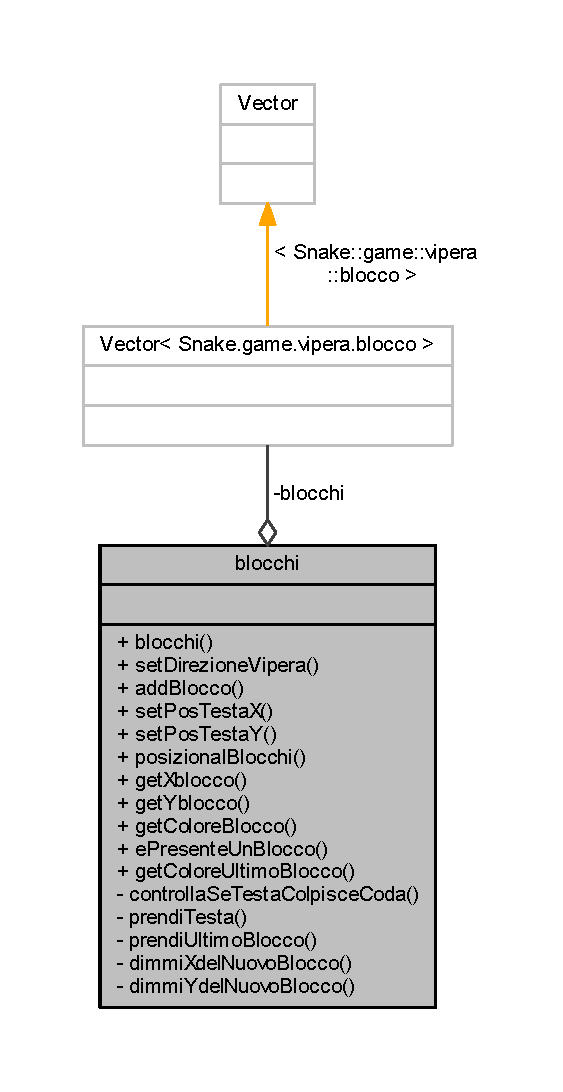
\includegraphics[width=270pt]{class_snake_1_1game_1_1vipera_1_1blocchi__coll__graph}
\end{center}
\end{figure}
\subsection*{Public Member Functions}
\begin{DoxyCompactItemize}
\item 
\mbox{\hyperlink{class_snake_1_1game_1_1vipera_1_1blocchi_af15f919c8bd034fb2f61735594958357}{blocchi}} (int startX, int startY)
\begin{DoxyCompactList}\small\item\em Costruttore con parametri della classe. \end{DoxyCompactList}\item 
void \mbox{\hyperlink{class_snake_1_1game_1_1vipera_1_1blocchi_a6007259ace9d33bd56b9a6193e86df39}{set\+Direzione\+Vipera}} (\mbox{\hyperlink{enum_snake_1_1game_1_1utility_1_1_directions}{Directions}} dir)
\begin{DoxyCompactList}\small\item\em Il metodo imposta la direzione della testa della vipera a seconda del parametro passato. \end{DoxyCompactList}\item 
void \mbox{\hyperlink{class_snake_1_1game_1_1vipera_1_1blocchi_aca08d818f8eb2849ca337ea2c64f344d}{add\+Blocco}} (Color colore\+Blocco)
\begin{DoxyCompactList}\small\item\em Il metodo aggiunge un blocco in coda alla vipera. \end{DoxyCompactList}\item 
void \mbox{\hyperlink{class_snake_1_1game_1_1vipera_1_1blocchi_a1e26556cba7802de510ce21bc9096149}{set\+Pos\+TestaX}} (int act\+Posx)
\begin{DoxyCompactList}\small\item\em Il metodo imposta la posizione X della testa della vipera a seconda del parametro passato. \end{DoxyCompactList}\item 
void \mbox{\hyperlink{class_snake_1_1game_1_1vipera_1_1blocchi_a7136da8bd75e6d0622eecf38aea1b60e}{set\+Pos\+TestaY}} (int act\+PosY)
\begin{DoxyCompactList}\small\item\em Il metodo imposta la posizione Y della testa della vipera a seconda del parametro passato. \end{DoxyCompactList}\item 
void \mbox{\hyperlink{class_snake_1_1game_1_1vipera_1_1blocchi_a2fbeb7ff9ae1fc1f5c5b1a885900034c}{posiziona\+I\+Blocchi}} ()
\begin{DoxyCompactList}\small\item\em Il metodo dice ad ogni blocco (ad eccezione della testa) di seguire il blocco davanti. \end{DoxyCompactList}\item 
int \mbox{\hyperlink{class_snake_1_1game_1_1vipera_1_1blocchi_ac25c5b310cb26c05d5ea69485d1e155f}{get\+Xblocco}} (int i)
\begin{DoxyCompactList}\small\item\em Il metodo ritorna la posizione X del blocco indicato come parametro. \end{DoxyCompactList}\item 
int \mbox{\hyperlink{class_snake_1_1game_1_1vipera_1_1blocchi_a4fad016a4b1de9e17b7092abd420d962}{get\+Yblocco}} (int i)
\begin{DoxyCompactList}\small\item\em Il metodo ritorna la posizione Y del blocco indicato come parametro. \end{DoxyCompactList}\item 
Color \mbox{\hyperlink{class_snake_1_1game_1_1vipera_1_1blocchi_a6c5d6f8c561308ff9ec579b370a969e0}{get\+Colore\+Blocco}} (int i)
\begin{DoxyCompactList}\small\item\em Il metodo ritorna il colore del blocco indicato come parametro. \end{DoxyCompactList}\item 
boolean \mbox{\hyperlink{class_snake_1_1game_1_1vipera_1_1blocchi_ac24833a417b3bd7c60e29ed5b7edc29f}{e\+Presente\+Un\+Blocco}} (int x, int y)
\begin{DoxyCompactList}\small\item\em Il metodo ritorna true se nella posizione X e Y passata come parametro e\textquotesingle{} presente un blocco della vipera. \end{DoxyCompactList}\item 
Color \mbox{\hyperlink{class_snake_1_1game_1_1vipera_1_1blocchi_a1afbc9b85396f53e6180eab2e5a36d4d}{get\+Colore\+Ultimo\+Blocco}} ()
\begin{DoxyCompactList}\small\item\em Il metodo ritorna il colore dell\textquotesingle{}ultimo blocco che compone la vipera. \end{DoxyCompactList}\end{DoxyCompactItemize}
\subsection*{Private Member Functions}
\begin{DoxyCompactItemize}
\item 
boolean \mbox{\hyperlink{class_snake_1_1game_1_1vipera_1_1blocchi_a1437df7b6446c67e0385922e99343857}{controlla\+Se\+Testa\+Colpisce\+Coda}} ()
\begin{DoxyCompactList}\small\item\em Il metodo controlla se la testa della vipera colpisce un blocco della sua coda. \end{DoxyCompactList}\item 
\mbox{\hyperlink{class_snake_1_1game_1_1vipera_1_1blocco}{blocco}} \mbox{\hyperlink{class_snake_1_1game_1_1vipera_1_1blocchi_a0479241855807563d1a7ed14bb5210cd}{prendi\+Testa}} ()
\begin{DoxyCompactList}\small\item\em Il metodo ritorna il blocco che corrisponde alla testa della vipera. \end{DoxyCompactList}\item 
\mbox{\hyperlink{class_snake_1_1game_1_1vipera_1_1blocco}{blocco}} \mbox{\hyperlink{class_snake_1_1game_1_1vipera_1_1blocchi_a31739bbc3222c3434ef9b45756523574}{prendi\+Ultimo\+Blocco}} ()
\begin{DoxyCompactList}\small\item\em Il metodo ritorna l\textquotesingle{}ultimo blocco che compone la vipera. \end{DoxyCompactList}\item 
int \mbox{\hyperlink{class_snake_1_1game_1_1vipera_1_1blocchi_afda852123016bddf1840fdb19241ffa3}{dimmi\+Xdel\+Nuovo\+Blocco}} ()
\begin{DoxyCompactList}\small\item\em Il metodo ritorna la posizione X dell\textquotesingle{}blocco che compone la vipera. \end{DoxyCompactList}\item 
int \mbox{\hyperlink{class_snake_1_1game_1_1vipera_1_1blocchi_a78a0129c937328d9bd0dafc68d007aef}{dimmi\+Ydel\+Nuovo\+Blocco}} ()
\begin{DoxyCompactList}\small\item\em Il metodo ritorna la posizione Y dell\textquotesingle{}blocco che compone la vipera. \end{DoxyCompactList}\end{DoxyCompactItemize}
\subsection*{Private Attributes}
\begin{DoxyCompactItemize}
\item 
Vector$<$ \mbox{\hyperlink{class_snake_1_1game_1_1vipera_1_1blocco}{blocco}} $>$ \mbox{\hyperlink{class_snake_1_1game_1_1vipera_1_1blocchi_ad6cdae3853215d2776147ba0c54ad406}{blocchi}} = new Vector$<$\mbox{\hyperlink{class_snake_1_1game_1_1vipera_1_1blocco}{blocco}}$>$()
\end{DoxyCompactItemize}


\subsection{Detailed Description}
\begin{DoxyAuthor}{Author}
Saccani Federico, \href{mailto:federico.saccani01@gmail.com}{\tt federico.\+saccani01@gmail.\+com} 
\end{DoxyAuthor}
\begin{DoxyVersion}{Version}
1.\+0 ~\newline
La classe rappresenta tutti i blocchi che compongono la vipera 
\end{DoxyVersion}


Definition at line 16 of file blocchi.\+java.



\subsection{Constructor \& Destructor Documentation}
\mbox{\Hypertarget{class_snake_1_1game_1_1vipera_1_1blocchi_af15f919c8bd034fb2f61735594958357}\label{class_snake_1_1game_1_1vipera_1_1blocchi_af15f919c8bd034fb2f61735594958357}} 
\index{Snake\+::game\+::vipera\+::blocchi@{Snake\+::game\+::vipera\+::blocchi}!blocchi@{blocchi}}
\index{blocchi@{blocchi}!Snake\+::game\+::vipera\+::blocchi@{Snake\+::game\+::vipera\+::blocchi}}
\subsubsection{\texorpdfstring{blocchi()}{blocchi()}}
{\footnotesize\ttfamily \mbox{\hyperlink{class_snake_1_1game_1_1vipera_1_1blocchi}{blocchi}} (\begin{DoxyParamCaption}\item[{int}]{startX,  }\item[{int}]{startY }\end{DoxyParamCaption})}



Costruttore con parametri della classe. 


\begin{DoxyParams}{Parameters}
{\em startX} & posizione X iniziale della testa \\
\hline
{\em startY} & posizione Y iniziale della testa \\
\hline
\end{DoxyParams}


Definition at line 26 of file blocchi.\+java.



\subsection{Member Function Documentation}
\mbox{\Hypertarget{class_snake_1_1game_1_1vipera_1_1blocchi_aca08d818f8eb2849ca337ea2c64f344d}\label{class_snake_1_1game_1_1vipera_1_1blocchi_aca08d818f8eb2849ca337ea2c64f344d}} 
\index{Snake\+::game\+::vipera\+::blocchi@{Snake\+::game\+::vipera\+::blocchi}!add\+Blocco@{add\+Blocco}}
\index{add\+Blocco@{add\+Blocco}!Snake\+::game\+::vipera\+::blocchi@{Snake\+::game\+::vipera\+::blocchi}}
\subsubsection{\texorpdfstring{add\+Blocco()}{addBlocco()}}
{\footnotesize\ttfamily void add\+Blocco (\begin{DoxyParamCaption}\item[{Color}]{colore\+Blocco }\end{DoxyParamCaption})}



Il metodo aggiunge un blocco in coda alla vipera. 


\begin{DoxyParams}{Parameters}
{\em colore\+Blocco} & colore del blocco da aggiungere \\
\hline
\end{DoxyParams}


Definition at line 88 of file blocchi.\+java.

Here is the call graph for this function\+:
\nopagebreak
\begin{figure}[H]
\begin{center}
\leavevmode
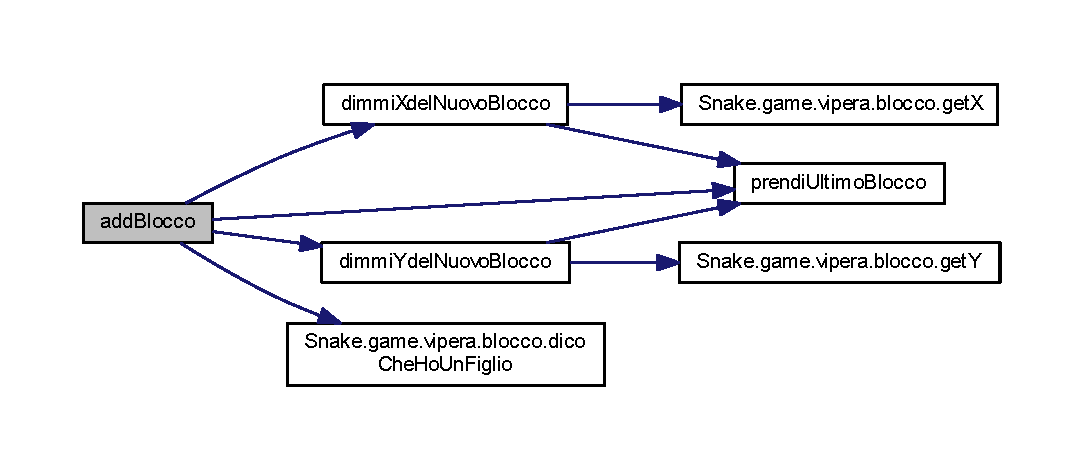
\includegraphics[width=350pt]{class_snake_1_1game_1_1vipera_1_1blocchi_aca08d818f8eb2849ca337ea2c64f344d_cgraph}
\end{center}
\end{figure}
Here is the caller graph for this function\+:
\nopagebreak
\begin{figure}[H]
\begin{center}
\leavevmode
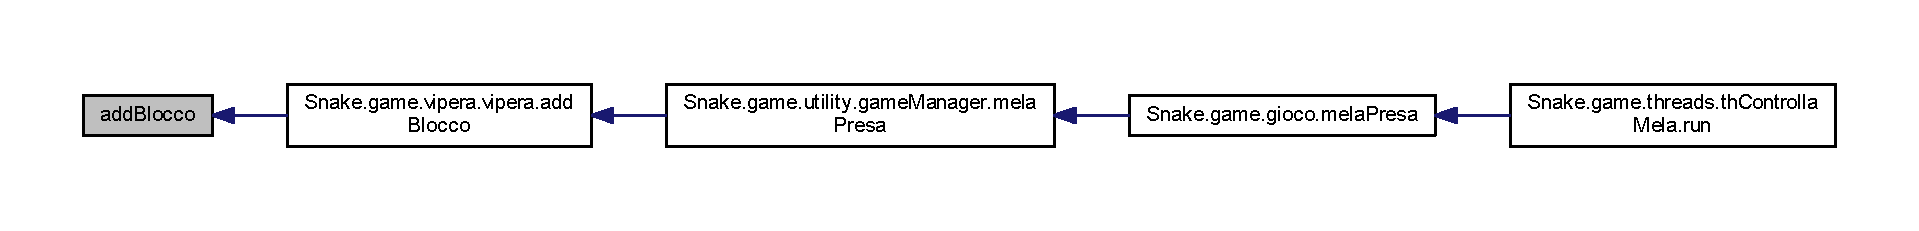
\includegraphics[width=350pt]{class_snake_1_1game_1_1vipera_1_1blocchi_aca08d818f8eb2849ca337ea2c64f344d_icgraph}
\end{center}
\end{figure}
\mbox{\Hypertarget{class_snake_1_1game_1_1vipera_1_1blocchi_a1437df7b6446c67e0385922e99343857}\label{class_snake_1_1game_1_1vipera_1_1blocchi_a1437df7b6446c67e0385922e99343857}} 
\index{Snake\+::game\+::vipera\+::blocchi@{Snake\+::game\+::vipera\+::blocchi}!controlla\+Se\+Testa\+Colpisce\+Coda@{controlla\+Se\+Testa\+Colpisce\+Coda}}
\index{controlla\+Se\+Testa\+Colpisce\+Coda@{controlla\+Se\+Testa\+Colpisce\+Coda}!Snake\+::game\+::vipera\+::blocchi@{Snake\+::game\+::vipera\+::blocchi}}
\subsubsection{\texorpdfstring{controlla\+Se\+Testa\+Colpisce\+Coda()}{controllaSeTestaColpisceCoda()}}
{\footnotesize\ttfamily boolean controlla\+Se\+Testa\+Colpisce\+Coda (\begin{DoxyParamCaption}{ }\end{DoxyParamCaption})\hspace{0.3cm}{\ttfamily [private]}}



Il metodo controlla se la testa della vipera colpisce un blocco della sua coda. 



Definition at line 47 of file blocchi.\+java.

Here is the call graph for this function\+:
\nopagebreak
\begin{figure}[H]
\begin{center}
\leavevmode
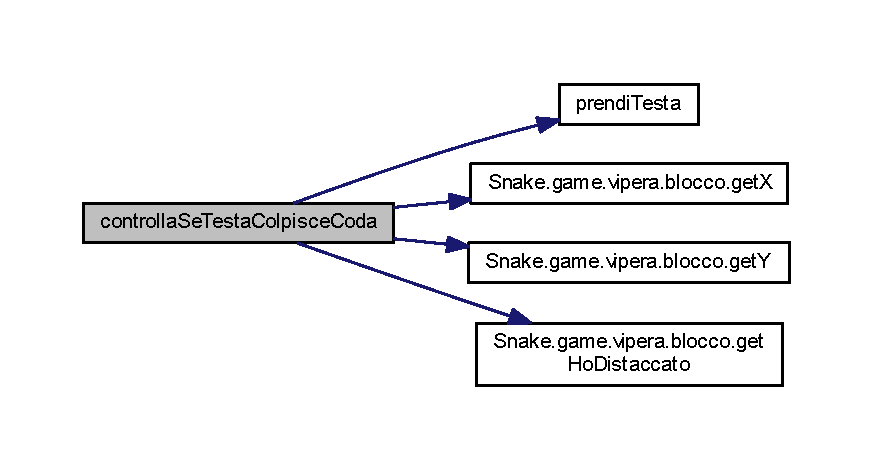
\includegraphics[width=350pt]{class_snake_1_1game_1_1vipera_1_1blocchi_a1437df7b6446c67e0385922e99343857_cgraph}
\end{center}
\end{figure}
Here is the caller graph for this function\+:
\nopagebreak
\begin{figure}[H]
\begin{center}
\leavevmode
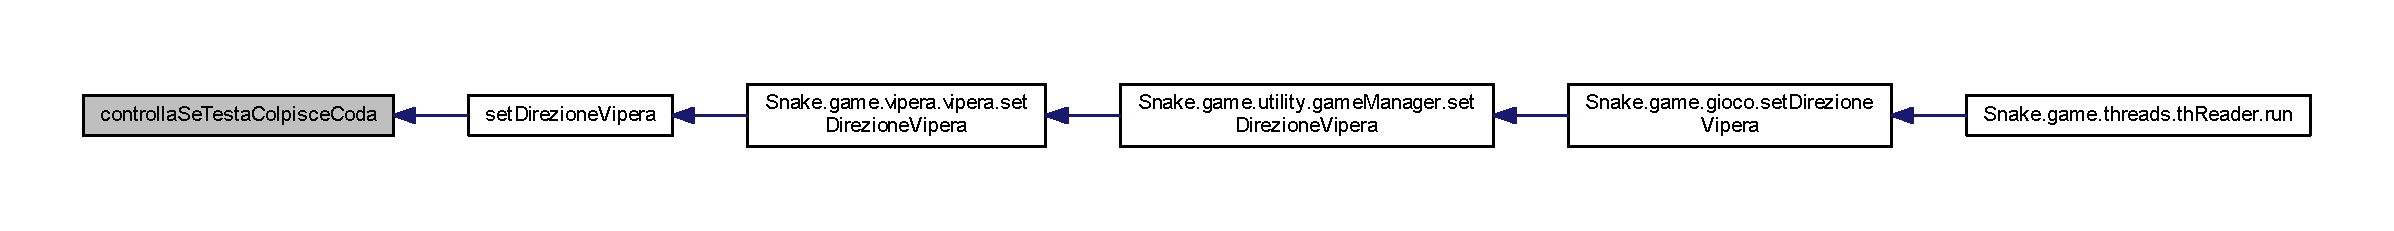
\includegraphics[width=350pt]{class_snake_1_1game_1_1vipera_1_1blocchi_a1437df7b6446c67e0385922e99343857_icgraph}
\end{center}
\end{figure}
\mbox{\Hypertarget{class_snake_1_1game_1_1vipera_1_1blocchi_afda852123016bddf1840fdb19241ffa3}\label{class_snake_1_1game_1_1vipera_1_1blocchi_afda852123016bddf1840fdb19241ffa3}} 
\index{Snake\+::game\+::vipera\+::blocchi@{Snake\+::game\+::vipera\+::blocchi}!dimmi\+Xdel\+Nuovo\+Blocco@{dimmi\+Xdel\+Nuovo\+Blocco}}
\index{dimmi\+Xdel\+Nuovo\+Blocco@{dimmi\+Xdel\+Nuovo\+Blocco}!Snake\+::game\+::vipera\+::blocchi@{Snake\+::game\+::vipera\+::blocchi}}
\subsubsection{\texorpdfstring{dimmi\+Xdel\+Nuovo\+Blocco()}{dimmiXdelNuovoBlocco()}}
{\footnotesize\ttfamily int dimmi\+Xdel\+Nuovo\+Blocco (\begin{DoxyParamCaption}{ }\end{DoxyParamCaption})\hspace{0.3cm}{\ttfamily [private]}}



Il metodo ritorna la posizione X dell\textquotesingle{}blocco che compone la vipera. 



Definition at line 120 of file blocchi.\+java.

Here is the call graph for this function\+:
\nopagebreak
\begin{figure}[H]
\begin{center}
\leavevmode
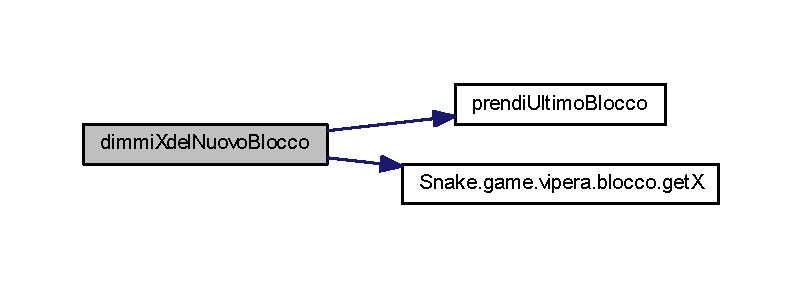
\includegraphics[width=350pt]{class_snake_1_1game_1_1vipera_1_1blocchi_afda852123016bddf1840fdb19241ffa3_cgraph}
\end{center}
\end{figure}
Here is the caller graph for this function\+:
\nopagebreak
\begin{figure}[H]
\begin{center}
\leavevmode
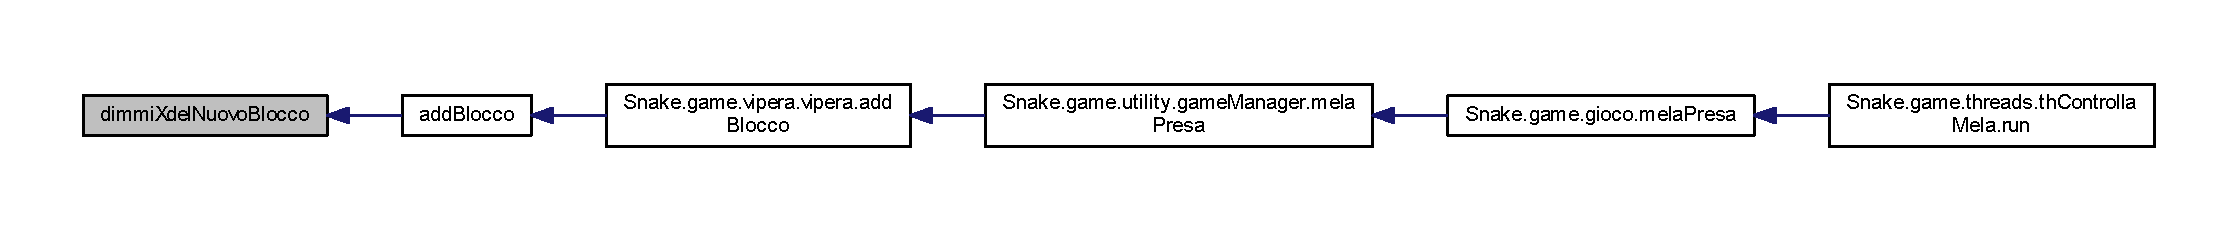
\includegraphics[width=350pt]{class_snake_1_1game_1_1vipera_1_1blocchi_afda852123016bddf1840fdb19241ffa3_icgraph}
\end{center}
\end{figure}
\mbox{\Hypertarget{class_snake_1_1game_1_1vipera_1_1blocchi_a78a0129c937328d9bd0dafc68d007aef}\label{class_snake_1_1game_1_1vipera_1_1blocchi_a78a0129c937328d9bd0dafc68d007aef}} 
\index{Snake\+::game\+::vipera\+::blocchi@{Snake\+::game\+::vipera\+::blocchi}!dimmi\+Ydel\+Nuovo\+Blocco@{dimmi\+Ydel\+Nuovo\+Blocco}}
\index{dimmi\+Ydel\+Nuovo\+Blocco@{dimmi\+Ydel\+Nuovo\+Blocco}!Snake\+::game\+::vipera\+::blocchi@{Snake\+::game\+::vipera\+::blocchi}}
\subsubsection{\texorpdfstring{dimmi\+Ydel\+Nuovo\+Blocco()}{dimmiYdelNuovoBlocco()}}
{\footnotesize\ttfamily int dimmi\+Ydel\+Nuovo\+Blocco (\begin{DoxyParamCaption}{ }\end{DoxyParamCaption})\hspace{0.3cm}{\ttfamily [private]}}



Il metodo ritorna la posizione Y dell\textquotesingle{}blocco che compone la vipera. 



Definition at line 127 of file blocchi.\+java.

Here is the call graph for this function\+:
\nopagebreak
\begin{figure}[H]
\begin{center}
\leavevmode
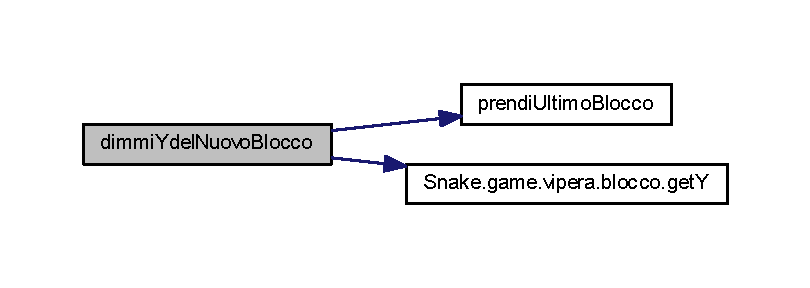
\includegraphics[width=350pt]{class_snake_1_1game_1_1vipera_1_1blocchi_a78a0129c937328d9bd0dafc68d007aef_cgraph}
\end{center}
\end{figure}
Here is the caller graph for this function\+:
\nopagebreak
\begin{figure}[H]
\begin{center}
\leavevmode
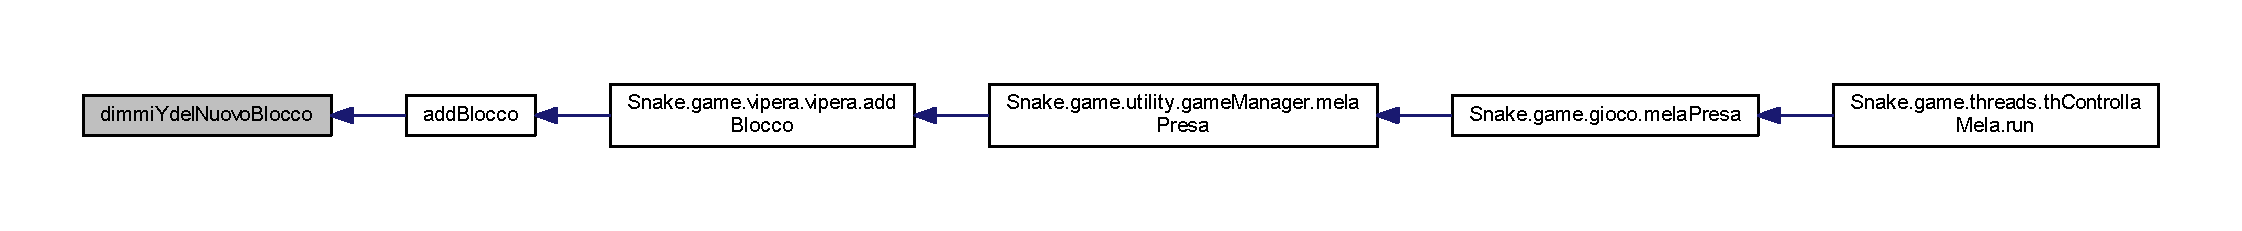
\includegraphics[width=350pt]{class_snake_1_1game_1_1vipera_1_1blocchi_a78a0129c937328d9bd0dafc68d007aef_icgraph}
\end{center}
\end{figure}
\mbox{\Hypertarget{class_snake_1_1game_1_1vipera_1_1blocchi_ac24833a417b3bd7c60e29ed5b7edc29f}\label{class_snake_1_1game_1_1vipera_1_1blocchi_ac24833a417b3bd7c60e29ed5b7edc29f}} 
\index{Snake\+::game\+::vipera\+::blocchi@{Snake\+::game\+::vipera\+::blocchi}!e\+Presente\+Un\+Blocco@{e\+Presente\+Un\+Blocco}}
\index{e\+Presente\+Un\+Blocco@{e\+Presente\+Un\+Blocco}!Snake\+::game\+::vipera\+::blocchi@{Snake\+::game\+::vipera\+::blocchi}}
\subsubsection{\texorpdfstring{e\+Presente\+Un\+Blocco()}{ePresenteUnBlocco()}}
{\footnotesize\ttfamily boolean e\+Presente\+Un\+Blocco (\begin{DoxyParamCaption}\item[{int}]{x,  }\item[{int}]{y }\end{DoxyParamCaption})}



Il metodo ritorna true se nella posizione X e Y passata come parametro e\textquotesingle{} presente un blocco della vipera. 


\begin{DoxyParams}{Parameters}
{\em x} & posizione x del blocco \\
\hline
{\em y} & posizione y del blocco \\
\hline
\end{DoxyParams}


Definition at line 201 of file blocchi.\+java.

Here is the caller graph for this function\+:
\nopagebreak
\begin{figure}[H]
\begin{center}
\leavevmode
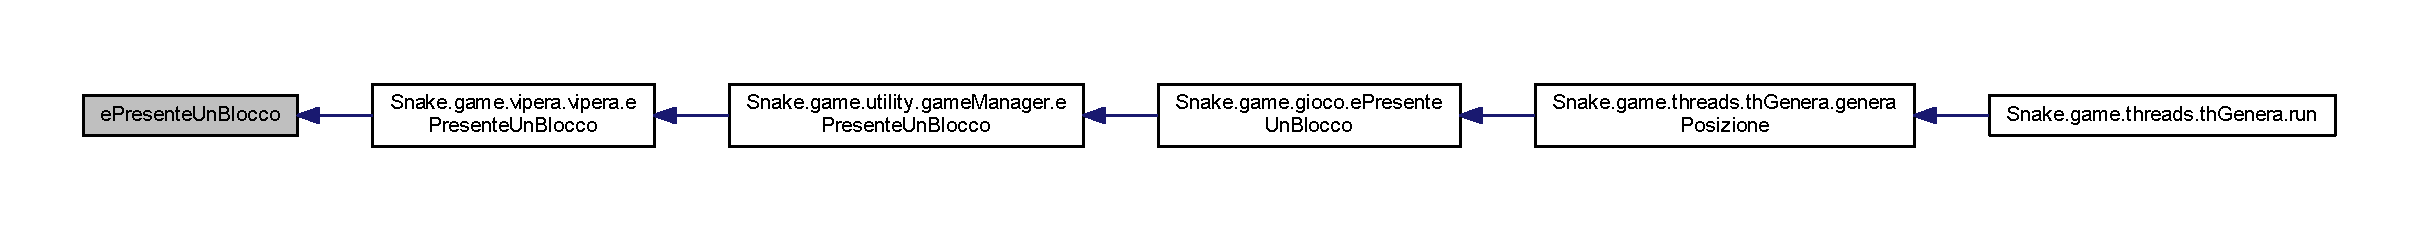
\includegraphics[width=350pt]{class_snake_1_1game_1_1vipera_1_1blocchi_ac24833a417b3bd7c60e29ed5b7edc29f_icgraph}
\end{center}
\end{figure}
\mbox{\Hypertarget{class_snake_1_1game_1_1vipera_1_1blocchi_a6c5d6f8c561308ff9ec579b370a969e0}\label{class_snake_1_1game_1_1vipera_1_1blocchi_a6c5d6f8c561308ff9ec579b370a969e0}} 
\index{Snake\+::game\+::vipera\+::blocchi@{Snake\+::game\+::vipera\+::blocchi}!get\+Colore\+Blocco@{get\+Colore\+Blocco}}
\index{get\+Colore\+Blocco@{get\+Colore\+Blocco}!Snake\+::game\+::vipera\+::blocchi@{Snake\+::game\+::vipera\+::blocchi}}
\subsubsection{\texorpdfstring{get\+Colore\+Blocco()}{getColoreBlocco()}}
{\footnotesize\ttfamily Color get\+Colore\+Blocco (\begin{DoxyParamCaption}\item[{int}]{i }\end{DoxyParamCaption})}



Il metodo ritorna il colore del blocco indicato come parametro. 


\begin{DoxyParams}{Parameters}
{\em i} & identificativo del blocco \\
\hline
\end{DoxyParams}


Definition at line 191 of file blocchi.\+java.

Here is the caller graph for this function\+:
\nopagebreak
\begin{figure}[H]
\begin{center}
\leavevmode
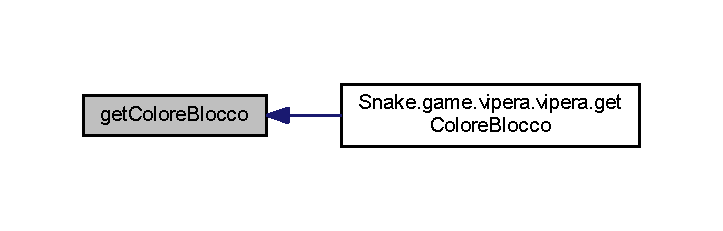
\includegraphics[width=347pt]{class_snake_1_1game_1_1vipera_1_1blocchi_a6c5d6f8c561308ff9ec579b370a969e0_icgraph}
\end{center}
\end{figure}
\mbox{\Hypertarget{class_snake_1_1game_1_1vipera_1_1blocchi_a1afbc9b85396f53e6180eab2e5a36d4d}\label{class_snake_1_1game_1_1vipera_1_1blocchi_a1afbc9b85396f53e6180eab2e5a36d4d}} 
\index{Snake\+::game\+::vipera\+::blocchi@{Snake\+::game\+::vipera\+::blocchi}!get\+Colore\+Ultimo\+Blocco@{get\+Colore\+Ultimo\+Blocco}}
\index{get\+Colore\+Ultimo\+Blocco@{get\+Colore\+Ultimo\+Blocco}!Snake\+::game\+::vipera\+::blocchi@{Snake\+::game\+::vipera\+::blocchi}}
\subsubsection{\texorpdfstring{get\+Colore\+Ultimo\+Blocco()}{getColoreUltimoBlocco()}}
{\footnotesize\ttfamily Color get\+Colore\+Ultimo\+Blocco (\begin{DoxyParamCaption}{ }\end{DoxyParamCaption})}



Il metodo ritorna il colore dell\textquotesingle{}ultimo blocco che compone la vipera. 



Definition at line 219 of file blocchi.\+java.

Here is the call graph for this function\+:
\nopagebreak
\begin{figure}[H]
\begin{center}
\leavevmode
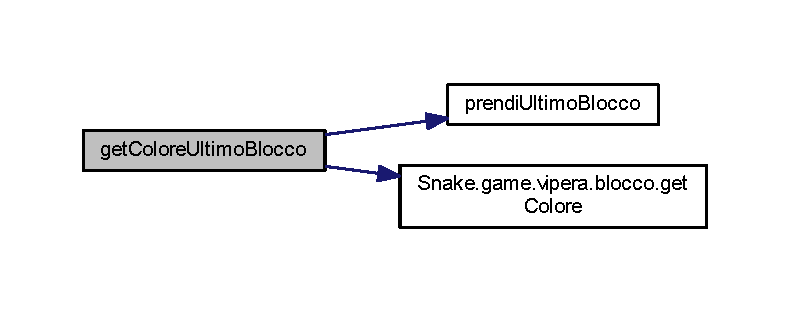
\includegraphics[width=350pt]{class_snake_1_1game_1_1vipera_1_1blocchi_a1afbc9b85396f53e6180eab2e5a36d4d_cgraph}
\end{center}
\end{figure}
Here is the caller graph for this function\+:
\nopagebreak
\begin{figure}[H]
\begin{center}
\leavevmode
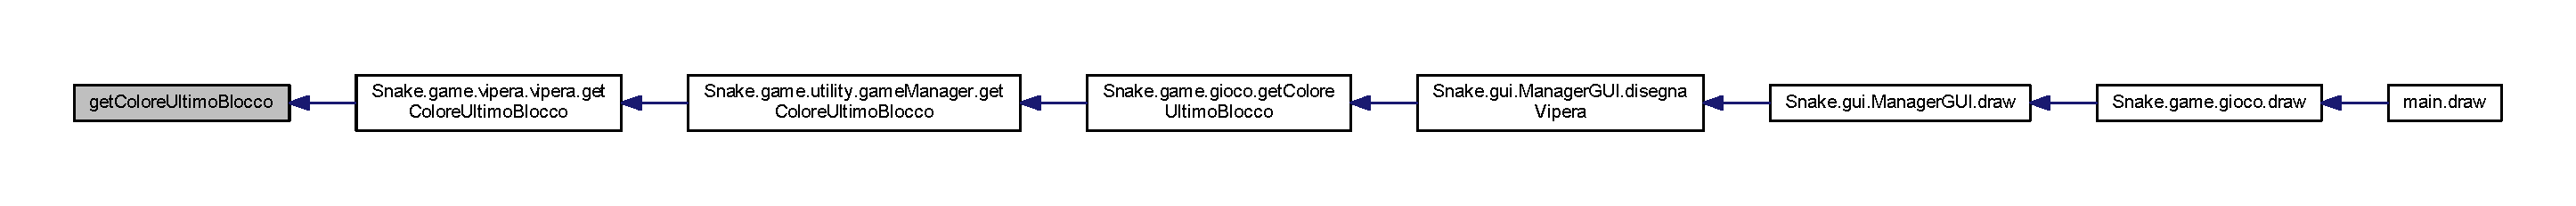
\includegraphics[width=350pt]{class_snake_1_1game_1_1vipera_1_1blocchi_a1afbc9b85396f53e6180eab2e5a36d4d_icgraph}
\end{center}
\end{figure}
\mbox{\Hypertarget{class_snake_1_1game_1_1vipera_1_1blocchi_ac25c5b310cb26c05d5ea69485d1e155f}\label{class_snake_1_1game_1_1vipera_1_1blocchi_ac25c5b310cb26c05d5ea69485d1e155f}} 
\index{Snake\+::game\+::vipera\+::blocchi@{Snake\+::game\+::vipera\+::blocchi}!get\+Xblocco@{get\+Xblocco}}
\index{get\+Xblocco@{get\+Xblocco}!Snake\+::game\+::vipera\+::blocchi@{Snake\+::game\+::vipera\+::blocchi}}
\subsubsection{\texorpdfstring{get\+Xblocco()}{getXblocco()}}
{\footnotesize\ttfamily int get\+Xblocco (\begin{DoxyParamCaption}\item[{int}]{i }\end{DoxyParamCaption})}



Il metodo ritorna la posizione X del blocco indicato come parametro. 


\begin{DoxyParams}{Parameters}
{\em i} & identificativo del blocco \\
\hline
\end{DoxyParams}


Definition at line 173 of file blocchi.\+java.

Here is the caller graph for this function\+:
\nopagebreak
\begin{figure}[H]
\begin{center}
\leavevmode
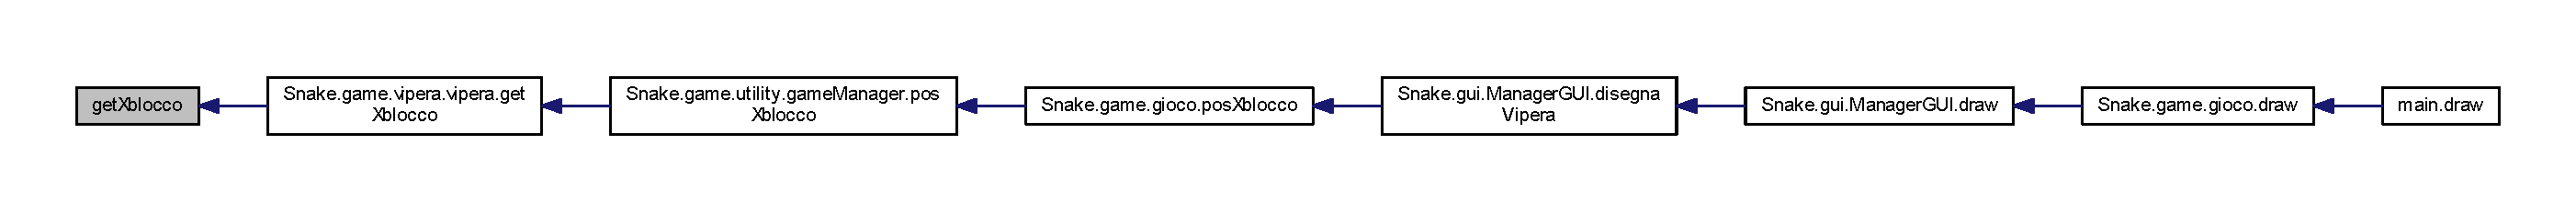
\includegraphics[width=350pt]{class_snake_1_1game_1_1vipera_1_1blocchi_ac25c5b310cb26c05d5ea69485d1e155f_icgraph}
\end{center}
\end{figure}
\mbox{\Hypertarget{class_snake_1_1game_1_1vipera_1_1blocchi_a4fad016a4b1de9e17b7092abd420d962}\label{class_snake_1_1game_1_1vipera_1_1blocchi_a4fad016a4b1de9e17b7092abd420d962}} 
\index{Snake\+::game\+::vipera\+::blocchi@{Snake\+::game\+::vipera\+::blocchi}!get\+Yblocco@{get\+Yblocco}}
\index{get\+Yblocco@{get\+Yblocco}!Snake\+::game\+::vipera\+::blocchi@{Snake\+::game\+::vipera\+::blocchi}}
\subsubsection{\texorpdfstring{get\+Yblocco()}{getYblocco()}}
{\footnotesize\ttfamily int get\+Yblocco (\begin{DoxyParamCaption}\item[{int}]{i }\end{DoxyParamCaption})}



Il metodo ritorna la posizione Y del blocco indicato come parametro. 


\begin{DoxyParams}{Parameters}
{\em i} & identificativo del blocco \\
\hline
\end{DoxyParams}


Definition at line 182 of file blocchi.\+java.

Here is the caller graph for this function\+:
\nopagebreak
\begin{figure}[H]
\begin{center}
\leavevmode
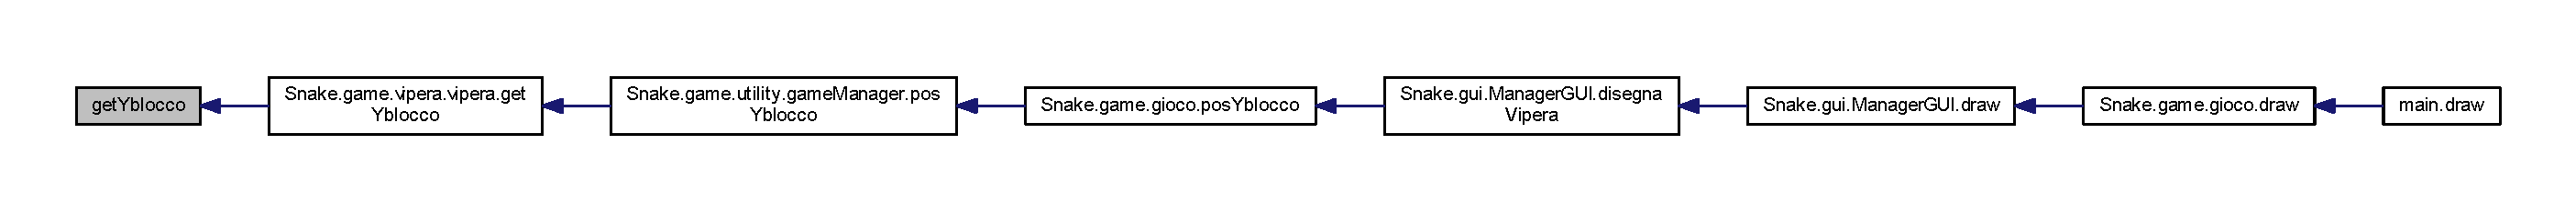
\includegraphics[width=350pt]{class_snake_1_1game_1_1vipera_1_1blocchi_a4fad016a4b1de9e17b7092abd420d962_icgraph}
\end{center}
\end{figure}
\mbox{\Hypertarget{class_snake_1_1game_1_1vipera_1_1blocchi_a2fbeb7ff9ae1fc1f5c5b1a885900034c}\label{class_snake_1_1game_1_1vipera_1_1blocchi_a2fbeb7ff9ae1fc1f5c5b1a885900034c}} 
\index{Snake\+::game\+::vipera\+::blocchi@{Snake\+::game\+::vipera\+::blocchi}!posiziona\+I\+Blocchi@{posiziona\+I\+Blocchi}}
\index{posiziona\+I\+Blocchi@{posiziona\+I\+Blocchi}!Snake\+::game\+::vipera\+::blocchi@{Snake\+::game\+::vipera\+::blocchi}}
\subsubsection{\texorpdfstring{posiziona\+I\+Blocchi()}{posizionaIBlocchi()}}
{\footnotesize\ttfamily void posiziona\+I\+Blocchi (\begin{DoxyParamCaption}{ }\end{DoxyParamCaption})}



Il metodo dice ad ogni blocco (ad eccezione della testa) di seguire il blocco davanti. 

In questo modo si crea l\textquotesingle{}effetto snake cioe\textquotesingle{} che i blocchi della coda seguono il percorso fatto dalla testa 

Definition at line 155 of file blocchi.\+java.

Here is the call graph for this function\+:
\nopagebreak
\begin{figure}[H]
\begin{center}
\leavevmode
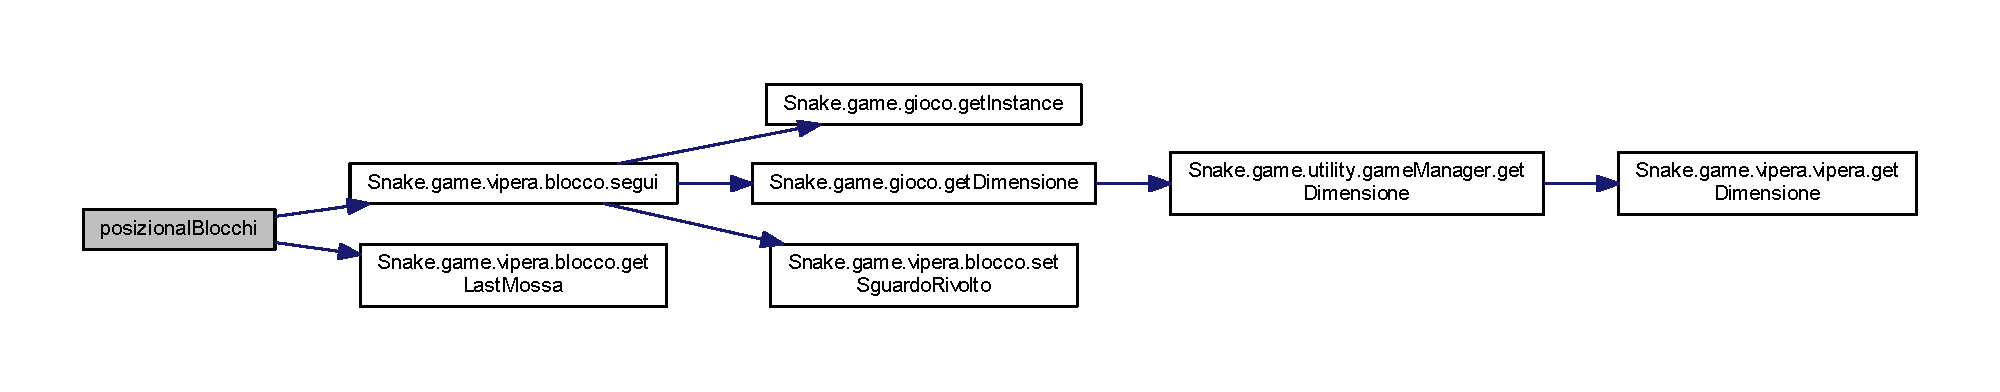
\includegraphics[width=350pt]{class_snake_1_1game_1_1vipera_1_1blocchi_a2fbeb7ff9ae1fc1f5c5b1a885900034c_cgraph}
\end{center}
\end{figure}
Here is the caller graph for this function\+:
\nopagebreak
\begin{figure}[H]
\begin{center}
\leavevmode
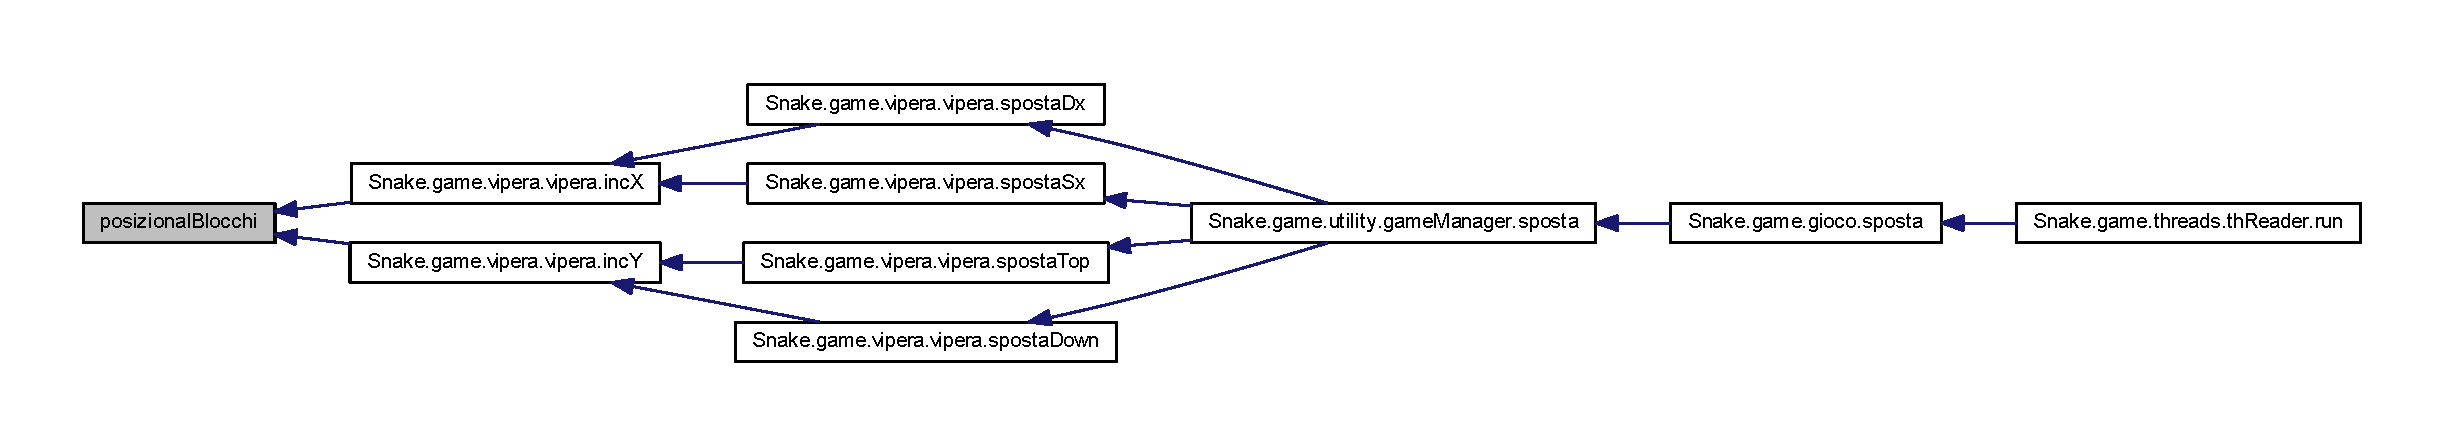
\includegraphics[width=350pt]{class_snake_1_1game_1_1vipera_1_1blocchi_a2fbeb7ff9ae1fc1f5c5b1a885900034c_icgraph}
\end{center}
\end{figure}
\mbox{\Hypertarget{class_snake_1_1game_1_1vipera_1_1blocchi_a0479241855807563d1a7ed14bb5210cd}\label{class_snake_1_1game_1_1vipera_1_1blocchi_a0479241855807563d1a7ed14bb5210cd}} 
\index{Snake\+::game\+::vipera\+::blocchi@{Snake\+::game\+::vipera\+::blocchi}!prendi\+Testa@{prendi\+Testa}}
\index{prendi\+Testa@{prendi\+Testa}!Snake\+::game\+::vipera\+::blocchi@{Snake\+::game\+::vipera\+::blocchi}}
\subsubsection{\texorpdfstring{prendi\+Testa()}{prendiTesta()}}
{\footnotesize\ttfamily \mbox{\hyperlink{class_snake_1_1game_1_1vipera_1_1blocco}{blocco}} prendi\+Testa (\begin{DoxyParamCaption}{ }\end{DoxyParamCaption})\hspace{0.3cm}{\ttfamily [private]}}



Il metodo ritorna il blocco che corrisponde alla testa della vipera. 



Definition at line 72 of file blocchi.\+java.

Here is the caller graph for this function\+:
\nopagebreak
\begin{figure}[H]
\begin{center}
\leavevmode
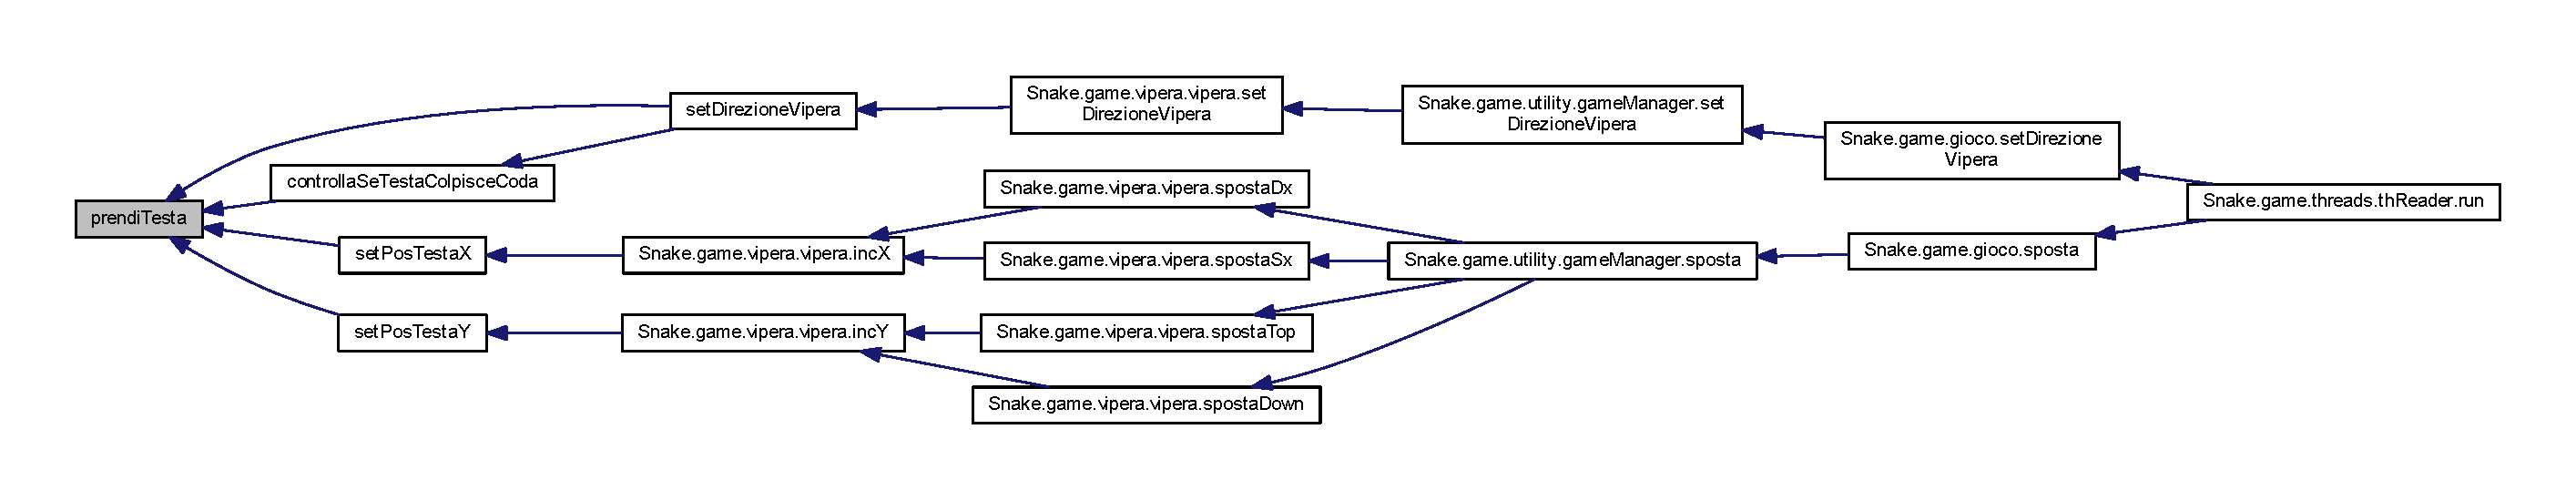
\includegraphics[width=350pt]{class_snake_1_1game_1_1vipera_1_1blocchi_a0479241855807563d1a7ed14bb5210cd_icgraph}
\end{center}
\end{figure}
\mbox{\Hypertarget{class_snake_1_1game_1_1vipera_1_1blocchi_a31739bbc3222c3434ef9b45756523574}\label{class_snake_1_1game_1_1vipera_1_1blocchi_a31739bbc3222c3434ef9b45756523574}} 
\index{Snake\+::game\+::vipera\+::blocchi@{Snake\+::game\+::vipera\+::blocchi}!prendi\+Ultimo\+Blocco@{prendi\+Ultimo\+Blocco}}
\index{prendi\+Ultimo\+Blocco@{prendi\+Ultimo\+Blocco}!Snake\+::game\+::vipera\+::blocchi@{Snake\+::game\+::vipera\+::blocchi}}
\subsubsection{\texorpdfstring{prendi\+Ultimo\+Blocco()}{prendiUltimoBlocco()}}
{\footnotesize\ttfamily \mbox{\hyperlink{class_snake_1_1game_1_1vipera_1_1blocco}{blocco}} prendi\+Ultimo\+Blocco (\begin{DoxyParamCaption}{ }\end{DoxyParamCaption})\hspace{0.3cm}{\ttfamily [private]}}



Il metodo ritorna l\textquotesingle{}ultimo blocco che compone la vipera. 



Definition at line 79 of file blocchi.\+java.

Here is the caller graph for this function\+:
\nopagebreak
\begin{figure}[H]
\begin{center}
\leavevmode
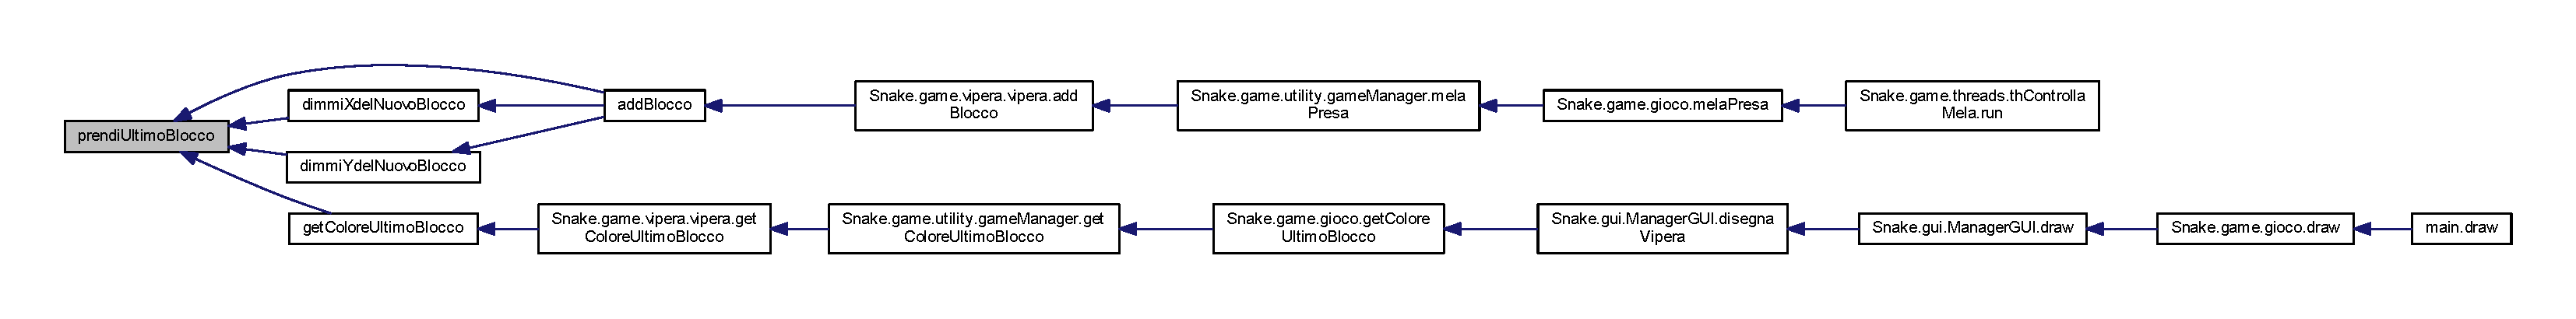
\includegraphics[width=350pt]{class_snake_1_1game_1_1vipera_1_1blocchi_a31739bbc3222c3434ef9b45756523574_icgraph}
\end{center}
\end{figure}
\mbox{\Hypertarget{class_snake_1_1game_1_1vipera_1_1blocchi_a6007259ace9d33bd56b9a6193e86df39}\label{class_snake_1_1game_1_1vipera_1_1blocchi_a6007259ace9d33bd56b9a6193e86df39}} 
\index{Snake\+::game\+::vipera\+::blocchi@{Snake\+::game\+::vipera\+::blocchi}!set\+Direzione\+Vipera@{set\+Direzione\+Vipera}}
\index{set\+Direzione\+Vipera@{set\+Direzione\+Vipera}!Snake\+::game\+::vipera\+::blocchi@{Snake\+::game\+::vipera\+::blocchi}}
\subsubsection{\texorpdfstring{set\+Direzione\+Vipera()}{setDirezioneVipera()}}
{\footnotesize\ttfamily void set\+Direzione\+Vipera (\begin{DoxyParamCaption}\item[{\mbox{\hyperlink{enum_snake_1_1game_1_1utility_1_1_directions}{Directions}}}]{dir }\end{DoxyParamCaption})}



Il metodo imposta la direzione della testa della vipera a seconda del parametro passato. 


\begin{DoxyParams}{Parameters}
{\em dir} & direzione testa \\
\hline
\end{DoxyParams}


Definition at line 36 of file blocchi.\+java.

Here is the call graph for this function\+:
\nopagebreak
\begin{figure}[H]
\begin{center}
\leavevmode
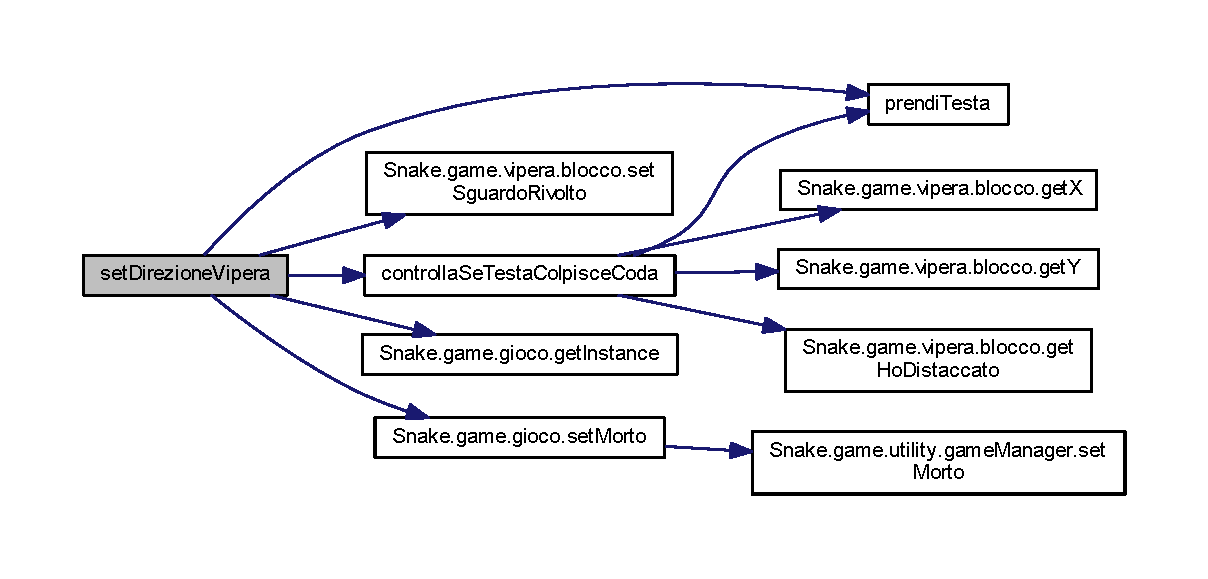
\includegraphics[width=350pt]{class_snake_1_1game_1_1vipera_1_1blocchi_a6007259ace9d33bd56b9a6193e86df39_cgraph}
\end{center}
\end{figure}
Here is the caller graph for this function\+:
\nopagebreak
\begin{figure}[H]
\begin{center}
\leavevmode
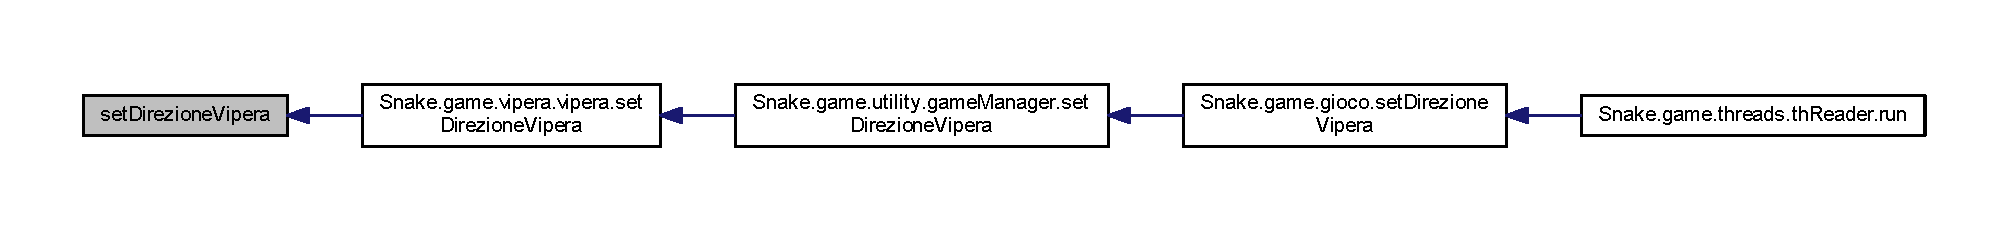
\includegraphics[width=350pt]{class_snake_1_1game_1_1vipera_1_1blocchi_a6007259ace9d33bd56b9a6193e86df39_icgraph}
\end{center}
\end{figure}
\mbox{\Hypertarget{class_snake_1_1game_1_1vipera_1_1blocchi_a1e26556cba7802de510ce21bc9096149}\label{class_snake_1_1game_1_1vipera_1_1blocchi_a1e26556cba7802de510ce21bc9096149}} 
\index{Snake\+::game\+::vipera\+::blocchi@{Snake\+::game\+::vipera\+::blocchi}!set\+Pos\+TestaX@{set\+Pos\+TestaX}}
\index{set\+Pos\+TestaX@{set\+Pos\+TestaX}!Snake\+::game\+::vipera\+::blocchi@{Snake\+::game\+::vipera\+::blocchi}}
\subsubsection{\texorpdfstring{set\+Pos\+Testa\+X()}{setPosTestaX()}}
{\footnotesize\ttfamily void set\+Pos\+TestaX (\begin{DoxyParamCaption}\item[{int}]{act\+Posx }\end{DoxyParamCaption})}



Il metodo imposta la posizione X della testa della vipera a seconda del parametro passato. 


\begin{DoxyParams}{Parameters}
{\em act\+Posx} & posizione X \\
\hline
\end{DoxyParams}


Definition at line 137 of file blocchi.\+java.

Here is the call graph for this function\+:
\nopagebreak
\begin{figure}[H]
\begin{center}
\leavevmode
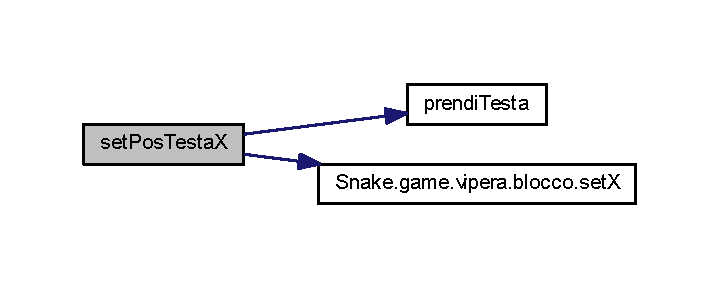
\includegraphics[width=345pt]{class_snake_1_1game_1_1vipera_1_1blocchi_a1e26556cba7802de510ce21bc9096149_cgraph}
\end{center}
\end{figure}
Here is the caller graph for this function\+:
\nopagebreak
\begin{figure}[H]
\begin{center}
\leavevmode
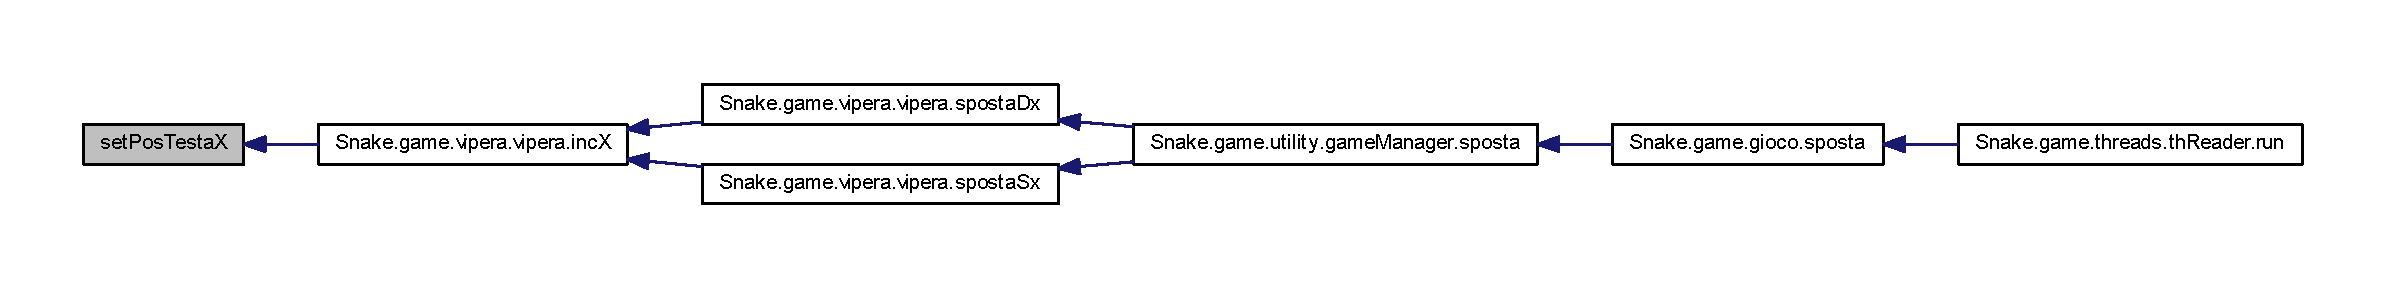
\includegraphics[width=350pt]{class_snake_1_1game_1_1vipera_1_1blocchi_a1e26556cba7802de510ce21bc9096149_icgraph}
\end{center}
\end{figure}
\mbox{\Hypertarget{class_snake_1_1game_1_1vipera_1_1blocchi_a7136da8bd75e6d0622eecf38aea1b60e}\label{class_snake_1_1game_1_1vipera_1_1blocchi_a7136da8bd75e6d0622eecf38aea1b60e}} 
\index{Snake\+::game\+::vipera\+::blocchi@{Snake\+::game\+::vipera\+::blocchi}!set\+Pos\+TestaY@{set\+Pos\+TestaY}}
\index{set\+Pos\+TestaY@{set\+Pos\+TestaY}!Snake\+::game\+::vipera\+::blocchi@{Snake\+::game\+::vipera\+::blocchi}}
\subsubsection{\texorpdfstring{set\+Pos\+Testa\+Y()}{setPosTestaY()}}
{\footnotesize\ttfamily void set\+Pos\+TestaY (\begin{DoxyParamCaption}\item[{int}]{act\+PosY }\end{DoxyParamCaption})}



Il metodo imposta la posizione Y della testa della vipera a seconda del parametro passato. 


\begin{DoxyParams}{Parameters}
{\em act\+PosY} & posizione Y \\
\hline
\end{DoxyParams}


Definition at line 146 of file blocchi.\+java.

Here is the call graph for this function\+:
\nopagebreak
\begin{figure}[H]
\begin{center}
\leavevmode
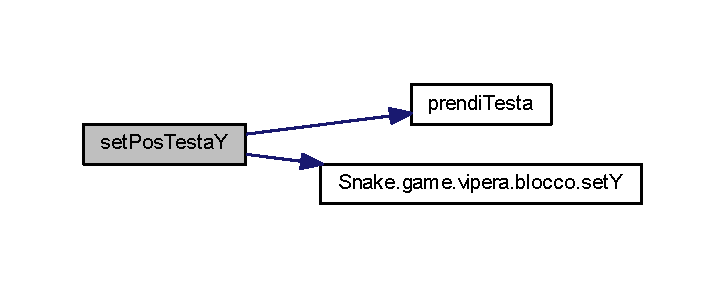
\includegraphics[width=348pt]{class_snake_1_1game_1_1vipera_1_1blocchi_a7136da8bd75e6d0622eecf38aea1b60e_cgraph}
\end{center}
\end{figure}
Here is the caller graph for this function\+:
\nopagebreak
\begin{figure}[H]
\begin{center}
\leavevmode
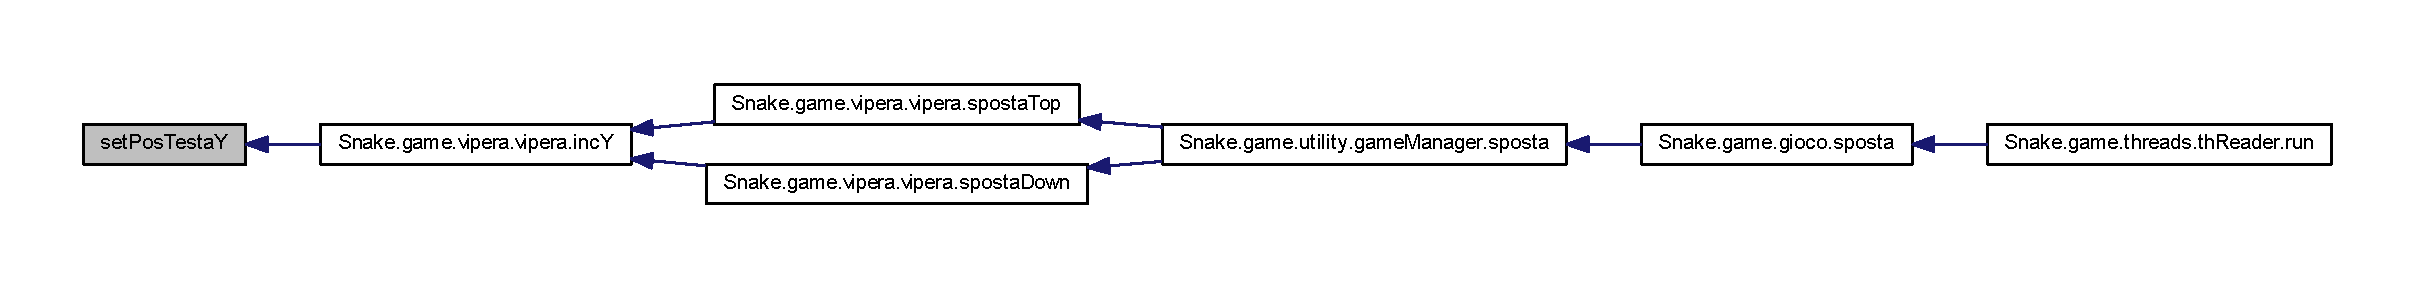
\includegraphics[width=350pt]{class_snake_1_1game_1_1vipera_1_1blocchi_a7136da8bd75e6d0622eecf38aea1b60e_icgraph}
\end{center}
\end{figure}


\subsection{Member Data Documentation}
\mbox{\Hypertarget{class_snake_1_1game_1_1vipera_1_1blocchi_ad6cdae3853215d2776147ba0c54ad406}\label{class_snake_1_1game_1_1vipera_1_1blocchi_ad6cdae3853215d2776147ba0c54ad406}} 
\index{Snake\+::game\+::vipera\+::blocchi@{Snake\+::game\+::vipera\+::blocchi}!blocchi@{blocchi}}
\index{blocchi@{blocchi}!Snake\+::game\+::vipera\+::blocchi@{Snake\+::game\+::vipera\+::blocchi}}
\subsubsection{\texorpdfstring{blocchi}{blocchi}}
{\footnotesize\ttfamily Vector$<$\mbox{\hyperlink{class_snake_1_1game_1_1vipera_1_1blocco}{blocco}}$>$ \mbox{\hyperlink{class_snake_1_1game_1_1vipera_1_1blocchi}{blocchi}} = new Vector$<$\mbox{\hyperlink{class_snake_1_1game_1_1vipera_1_1blocco}{blocco}}$>$()\hspace{0.3cm}{\ttfamily [private]}}

Attributo che rappresenta tutti i blocchi 

Definition at line 18 of file blocchi.\+java.



The documentation for this class was generated from the following file\+:\begin{DoxyCompactItemize}
\item 
src/main/java/\+Snake/game/vipera/\mbox{\hyperlink{blocchi_8java}{blocchi.\+java}}\end{DoxyCompactItemize}

\hypertarget{class_snake_1_1game_1_1vipera_1_1blocco}{}\section{blocco Class Reference}
\label{class_snake_1_1game_1_1vipera_1_1blocco}\index{blocco@{blocco}}


Collaboration diagram for blocco\+:
\nopagebreak
\begin{figure}[H]
\begin{center}
\leavevmode
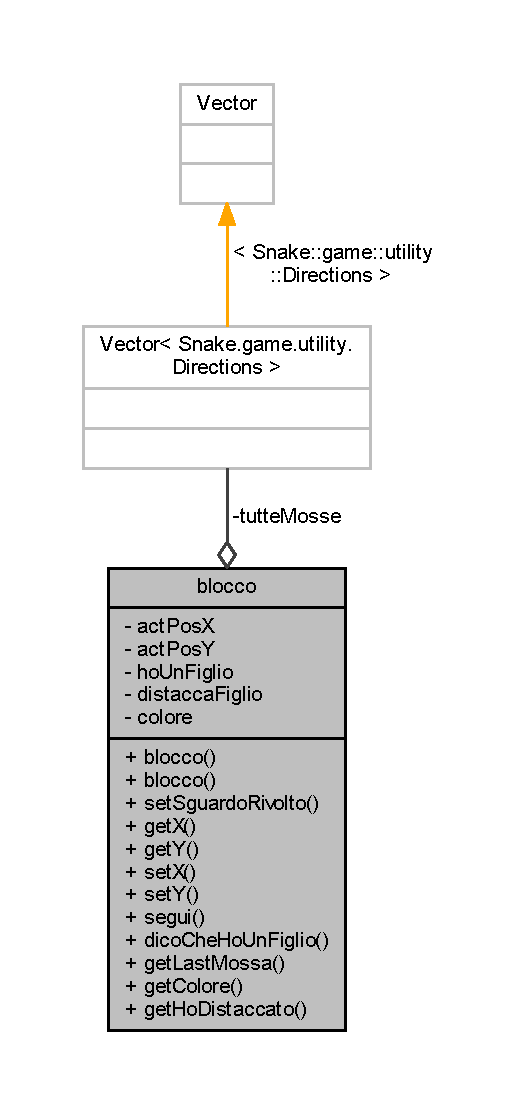
\includegraphics[width=249pt]{class_snake_1_1game_1_1vipera_1_1blocco__coll__graph}
\end{center}
\end{figure}
\subsection*{Public Member Functions}
\begin{DoxyCompactItemize}
\item 
\mbox{\hyperlink{class_snake_1_1game_1_1vipera_1_1blocco_a0143d1efd3c540135c872d58b6b2870d}{blocco}} ()
\begin{DoxyCompactList}\small\item\em Costruttore senza parametri della classe. \end{DoxyCompactList}\item 
\mbox{\hyperlink{class_snake_1_1game_1_1vipera_1_1blocco_a82f454d7ab34406585d65424866b6265}{blocco}} (int startX, int startY, Color \mbox{\hyperlink{class_snake_1_1game_1_1vipera_1_1blocco_ada0bf0be39e4ad9d58f6e7c48f14c64a}{colore}})
\begin{DoxyCompactList}\small\item\em Costruttore con parametri della classe. \end{DoxyCompactList}\item 
void \mbox{\hyperlink{class_snake_1_1game_1_1vipera_1_1blocco_a2d20c8ebc9efc39ed12392e6486d50d9}{set\+Sguardo\+Rivolto}} (\mbox{\hyperlink{enum_snake_1_1game_1_1utility_1_1_directions}{Directions}} dir)
\begin{DoxyCompactList}\small\item\em Il metodo permette di aggiornare l\textquotesingle{}attributo tutte\+Mosse a seconda della direzione passata come parametro. \end{DoxyCompactList}\item 
int \mbox{\hyperlink{class_snake_1_1game_1_1vipera_1_1blocco_ae13f88e922e1339355456062ad9fa359}{getX}} ()
\begin{DoxyCompactList}\small\item\em Ritorna la posizione X del blocco. \end{DoxyCompactList}\item 
int \mbox{\hyperlink{class_snake_1_1game_1_1vipera_1_1blocco_aab81944f0a14bba932c0931899951937}{getY}} ()
\begin{DoxyCompactList}\small\item\em Ritorna la posizione Y del blocco. \end{DoxyCompactList}\item 
void \mbox{\hyperlink{class_snake_1_1game_1_1vipera_1_1blocco_ab5a3acb0391238ee37a5da898bffd5f1}{setX}} (int \mbox{\hyperlink{class_snake_1_1game_1_1vipera_1_1blocco_aaa64105e6cedf2b98a63e3ab8c8f4cdb}{act\+PosX}})
\begin{DoxyCompactList}\small\item\em Imposta la posizione X del blocco a seconda del parametro. \end{DoxyCompactList}\item 
void \mbox{\hyperlink{class_snake_1_1game_1_1vipera_1_1blocco_a60e970e880a18799c14e771afe3e904b}{setY}} (int \mbox{\hyperlink{class_snake_1_1game_1_1vipera_1_1blocco_a301b22c6bff25f4530e3f991788338fe}{act\+PosY}})
\begin{DoxyCompactList}\small\item\em Imposta la posizione Y del blocco a seconda del parametro. \end{DoxyCompactList}\item 
void \mbox{\hyperlink{class_snake_1_1game_1_1vipera_1_1blocco_acabc02ee9509cd1e196033348dd76a6f}{segui}} (\mbox{\hyperlink{enum_snake_1_1game_1_1utility_1_1_directions}{Directions}} dove\+Vado)
\begin{DoxyCompactList}\small\item\em Il metodo permette di far muovere il blocco a seconda della direzione passata come parametro. \end{DoxyCompactList}\item 
void \mbox{\hyperlink{class_snake_1_1game_1_1vipera_1_1blocco_a7380314c5c58350a175d844e7121d329}{dico\+Che\+Ho\+Un\+Figlio}} ()
\begin{DoxyCompactList}\small\item\em Il metodo quando richiamato permette di far sapere al blocco attuale che e\textquotesingle{} stato generato un blocco in sua corrispondenza. \end{DoxyCompactList}\item 
\mbox{\hyperlink{enum_snake_1_1game_1_1utility_1_1_directions}{Directions}} \mbox{\hyperlink{class_snake_1_1game_1_1vipera_1_1blocco_a95fdd903a87a54ceaba0674eee0a4dda}{get\+Last\+Mossa}} ()
\begin{DoxyCompactList}\small\item\em Il metodo ritorna l\textquotesingle{}ultima mossa effettuata dal blocco attraverso una pop. \end{DoxyCompactList}\item 
Color \mbox{\hyperlink{class_snake_1_1game_1_1vipera_1_1blocco_ae3f520a7be49ba6d662a1504fbe4acf3}{get\+Colore}} ()
\begin{DoxyCompactList}\small\item\em Il metodo ritorna il colore del blocco. \end{DoxyCompactList}\item 
boolean \mbox{\hyperlink{class_snake_1_1game_1_1vipera_1_1blocco_a09b5923541116b960ee0c349c60b92fe}{get\+Ho\+Distaccato}} ()
\begin{DoxyCompactList}\small\item\em Il metodo ritorna l\textquotesingle{}attributo distacca\+Figlio. \end{DoxyCompactList}\end{DoxyCompactItemize}
\subsection*{Private Attributes}
\begin{DoxyCompactItemize}
\item 
int \mbox{\hyperlink{class_snake_1_1game_1_1vipera_1_1blocco_aaa64105e6cedf2b98a63e3ab8c8f4cdb}{act\+PosX}}
\item 
int \mbox{\hyperlink{class_snake_1_1game_1_1vipera_1_1blocco_a301b22c6bff25f4530e3f991788338fe}{act\+PosY}}
\item 
Vector$<$ \mbox{\hyperlink{enum_snake_1_1game_1_1utility_1_1_directions}{Directions}} $>$ \mbox{\hyperlink{class_snake_1_1game_1_1vipera_1_1blocco_a0670f48287135d82c64441e965d35c18}{tutte\+Mosse}} = new Vector$<$\mbox{\hyperlink{enum_snake_1_1game_1_1utility_1_1_directions}{Directions}}$>$()
\item 
boolean \mbox{\hyperlink{class_snake_1_1game_1_1vipera_1_1blocco_a909ed9e20b51021224373cb7e95365e7}{ho\+Un\+Figlio}}
\item 
boolean \mbox{\hyperlink{class_snake_1_1game_1_1vipera_1_1blocco_aab706c0c0218d17f9386c9dce8989195}{distacca\+Figlio}}
\item 
Color \mbox{\hyperlink{class_snake_1_1game_1_1vipera_1_1blocco_ada0bf0be39e4ad9d58f6e7c48f14c64a}{colore}}
\end{DoxyCompactItemize}


\subsection{Detailed Description}
\begin{DoxyAuthor}{Author}
Saccani Federico, \href{mailto:federico.saccani01@gmail.com}{\tt federico.\+saccani01@gmail.\+com} 
\end{DoxyAuthor}
\begin{DoxyVersion}{Version}
1.\+0 ~\newline
La classe corrisponde ad un blocco che compone la struttura della vipera 
\end{DoxyVersion}


Definition at line 15 of file blocco.\+java.



\subsection{Constructor \& Destructor Documentation}
\mbox{\Hypertarget{class_snake_1_1game_1_1vipera_1_1blocco_a0143d1efd3c540135c872d58b6b2870d}\label{class_snake_1_1game_1_1vipera_1_1blocco_a0143d1efd3c540135c872d58b6b2870d}} 
\index{Snake\+::game\+::vipera\+::blocco@{Snake\+::game\+::vipera\+::blocco}!blocco@{blocco}}
\index{blocco@{blocco}!Snake\+::game\+::vipera\+::blocco@{Snake\+::game\+::vipera\+::blocco}}
\subsubsection{\texorpdfstring{blocco()}{blocco()}\hspace{0.1cm}{\footnotesize\ttfamily [1/2]}}
{\footnotesize\ttfamily \mbox{\hyperlink{class_snake_1_1game_1_1vipera_1_1blocco}{blocco}} (\begin{DoxyParamCaption}{ }\end{DoxyParamCaption})}



Costruttore senza parametri della classe. 

Quando chiamato, imposta gli attributi della classi a valori di default 

Definition at line 38 of file blocco.\+java.

\mbox{\Hypertarget{class_snake_1_1game_1_1vipera_1_1blocco_a82f454d7ab34406585d65424866b6265}\label{class_snake_1_1game_1_1vipera_1_1blocco_a82f454d7ab34406585d65424866b6265}} 
\index{Snake\+::game\+::vipera\+::blocco@{Snake\+::game\+::vipera\+::blocco}!blocco@{blocco}}
\index{blocco@{blocco}!Snake\+::game\+::vipera\+::blocco@{Snake\+::game\+::vipera\+::blocco}}
\subsubsection{\texorpdfstring{blocco()}{blocco()}\hspace{0.1cm}{\footnotesize\ttfamily [2/2]}}
{\footnotesize\ttfamily \mbox{\hyperlink{class_snake_1_1game_1_1vipera_1_1blocco}{blocco}} (\begin{DoxyParamCaption}\item[{int}]{startX,  }\item[{int}]{startY,  }\item[{Color}]{colore }\end{DoxyParamCaption})}



Costruttore con parametri della classe. 

Imposta gli attributi della classe a seconda dei parametri passati


\begin{DoxyParams}{Parameters}
{\em startX} & posizione dell\textquotesingle{}asse X iniziale \\
\hline
{\em startY} & posizione dell\textquotesingle{}asse Y iniziale \\
\hline
{\em colore} & colore del blocco \\
\hline
\end{DoxyParams}


Definition at line 55 of file blocco.\+java.



\subsection{Member Function Documentation}
\mbox{\Hypertarget{class_snake_1_1game_1_1vipera_1_1blocco_a7380314c5c58350a175d844e7121d329}\label{class_snake_1_1game_1_1vipera_1_1blocco_a7380314c5c58350a175d844e7121d329}} 
\index{Snake\+::game\+::vipera\+::blocco@{Snake\+::game\+::vipera\+::blocco}!dico\+Che\+Ho\+Un\+Figlio@{dico\+Che\+Ho\+Un\+Figlio}}
\index{dico\+Che\+Ho\+Un\+Figlio@{dico\+Che\+Ho\+Un\+Figlio}!Snake\+::game\+::vipera\+::blocco@{Snake\+::game\+::vipera\+::blocco}}
\subsubsection{\texorpdfstring{dico\+Che\+Ho\+Un\+Figlio()}{dicoCheHoUnFiglio()}}
{\footnotesize\ttfamily void dico\+Che\+Ho\+Un\+Figlio (\begin{DoxyParamCaption}{ }\end{DoxyParamCaption})}



Il metodo quando richiamato permette di far sapere al blocco attuale che e\textquotesingle{} stato generato un blocco in sua corrispondenza. 



Definition at line 156 of file blocco.\+java.

Here is the caller graph for this function\+:
\nopagebreak
\begin{figure}[H]
\begin{center}
\leavevmode
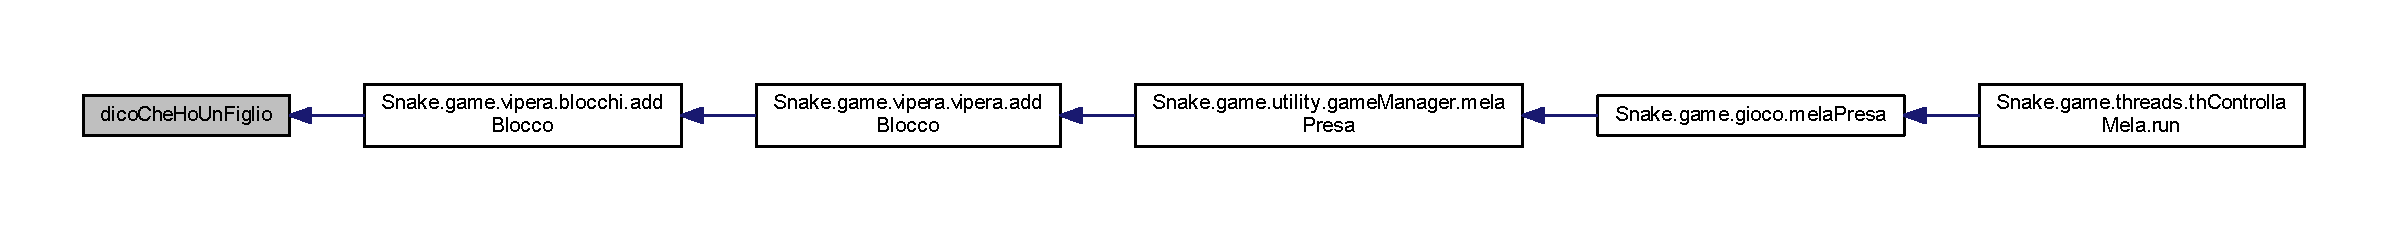
\includegraphics[width=350pt]{class_snake_1_1game_1_1vipera_1_1blocco_a7380314c5c58350a175d844e7121d329_icgraph}
\end{center}
\end{figure}
\mbox{\Hypertarget{class_snake_1_1game_1_1vipera_1_1blocco_ae3f520a7be49ba6d662a1504fbe4acf3}\label{class_snake_1_1game_1_1vipera_1_1blocco_ae3f520a7be49ba6d662a1504fbe4acf3}} 
\index{Snake\+::game\+::vipera\+::blocco@{Snake\+::game\+::vipera\+::blocco}!get\+Colore@{get\+Colore}}
\index{get\+Colore@{get\+Colore}!Snake\+::game\+::vipera\+::blocco@{Snake\+::game\+::vipera\+::blocco}}
\subsubsection{\texorpdfstring{get\+Colore()}{getColore()}}
{\footnotesize\ttfamily Color get\+Colore (\begin{DoxyParamCaption}{ }\end{DoxyParamCaption})}



Il metodo ritorna il colore del blocco. 



Definition at line 178 of file blocco.\+java.

Here is the caller graph for this function\+:
\nopagebreak
\begin{figure}[H]
\begin{center}
\leavevmode
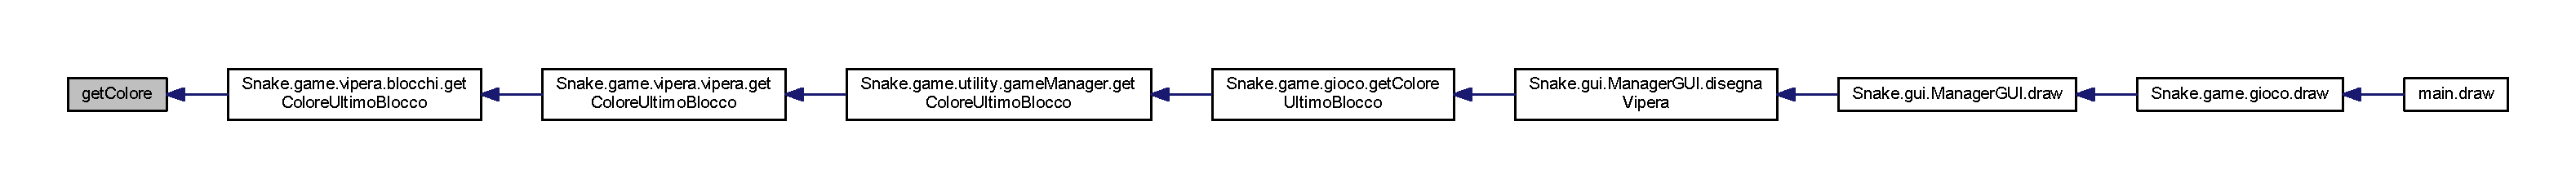
\includegraphics[width=350pt]{class_snake_1_1game_1_1vipera_1_1blocco_ae3f520a7be49ba6d662a1504fbe4acf3_icgraph}
\end{center}
\end{figure}
\mbox{\Hypertarget{class_snake_1_1game_1_1vipera_1_1blocco_a09b5923541116b960ee0c349c60b92fe}\label{class_snake_1_1game_1_1vipera_1_1blocco_a09b5923541116b960ee0c349c60b92fe}} 
\index{Snake\+::game\+::vipera\+::blocco@{Snake\+::game\+::vipera\+::blocco}!get\+Ho\+Distaccato@{get\+Ho\+Distaccato}}
\index{get\+Ho\+Distaccato@{get\+Ho\+Distaccato}!Snake\+::game\+::vipera\+::blocco@{Snake\+::game\+::vipera\+::blocco}}
\subsubsection{\texorpdfstring{get\+Ho\+Distaccato()}{getHoDistaccato()}}
{\footnotesize\ttfamily boolean get\+Ho\+Distaccato (\begin{DoxyParamCaption}{ }\end{DoxyParamCaption})}



Il metodo ritorna l\textquotesingle{}attributo distacca\+Figlio. 



Definition at line 185 of file blocco.\+java.

Here is the caller graph for this function\+:
\nopagebreak
\begin{figure}[H]
\begin{center}
\leavevmode
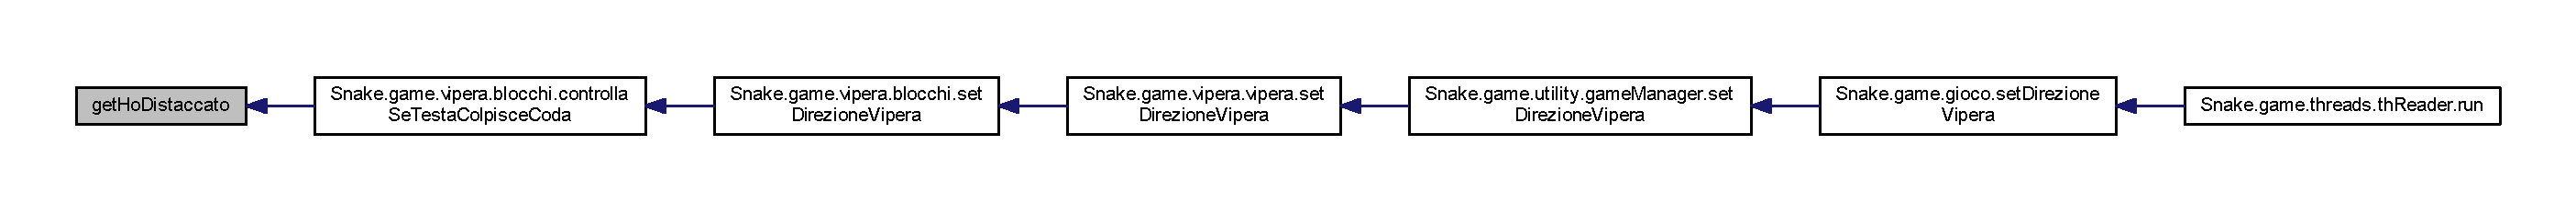
\includegraphics[width=350pt]{class_snake_1_1game_1_1vipera_1_1blocco_a09b5923541116b960ee0c349c60b92fe_icgraph}
\end{center}
\end{figure}
\mbox{\Hypertarget{class_snake_1_1game_1_1vipera_1_1blocco_a95fdd903a87a54ceaba0674eee0a4dda}\label{class_snake_1_1game_1_1vipera_1_1blocco_a95fdd903a87a54ceaba0674eee0a4dda}} 
\index{Snake\+::game\+::vipera\+::blocco@{Snake\+::game\+::vipera\+::blocco}!get\+Last\+Mossa@{get\+Last\+Mossa}}
\index{get\+Last\+Mossa@{get\+Last\+Mossa}!Snake\+::game\+::vipera\+::blocco@{Snake\+::game\+::vipera\+::blocco}}
\subsubsection{\texorpdfstring{get\+Last\+Mossa()}{getLastMossa()}}
{\footnotesize\ttfamily \mbox{\hyperlink{enum_snake_1_1game_1_1utility_1_1_directions}{Directions}} get\+Last\+Mossa (\begin{DoxyParamCaption}{ }\end{DoxyParamCaption})}



Il metodo ritorna l\textquotesingle{}ultima mossa effettuata dal blocco attraverso una pop. 



Definition at line 169 of file blocco.\+java.

Here is the caller graph for this function\+:
\nopagebreak
\begin{figure}[H]
\begin{center}
\leavevmode
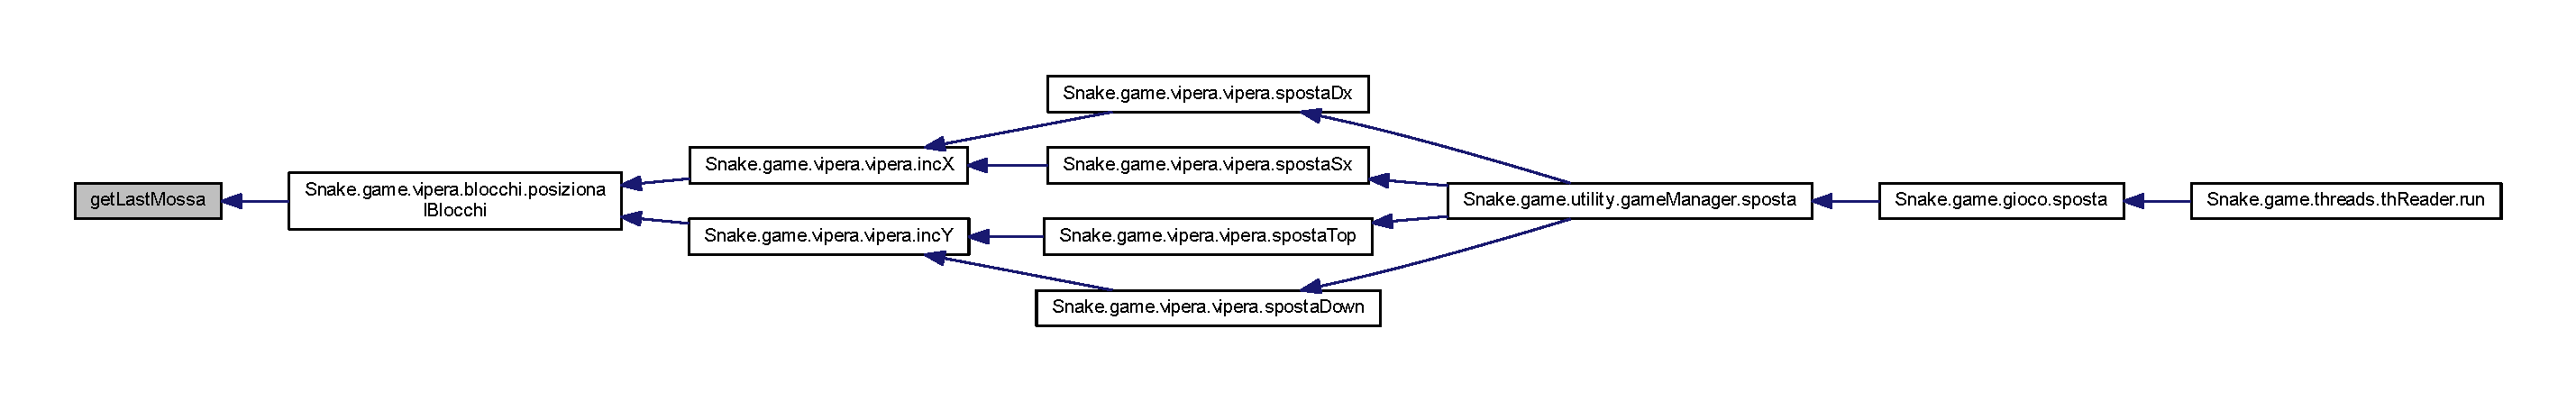
\includegraphics[width=350pt]{class_snake_1_1game_1_1vipera_1_1blocco_a95fdd903a87a54ceaba0674eee0a4dda_icgraph}
\end{center}
\end{figure}
\mbox{\Hypertarget{class_snake_1_1game_1_1vipera_1_1blocco_ae13f88e922e1339355456062ad9fa359}\label{class_snake_1_1game_1_1vipera_1_1blocco_ae13f88e922e1339355456062ad9fa359}} 
\index{Snake\+::game\+::vipera\+::blocco@{Snake\+::game\+::vipera\+::blocco}!getX@{getX}}
\index{getX@{getX}!Snake\+::game\+::vipera\+::blocco@{Snake\+::game\+::vipera\+::blocco}}
\subsubsection{\texorpdfstring{get\+X()}{getX()}}
{\footnotesize\ttfamily int getX (\begin{DoxyParamCaption}{ }\end{DoxyParamCaption})}



Ritorna la posizione X del blocco. 



Definition at line 95 of file blocco.\+java.

Here is the caller graph for this function\+:
\nopagebreak
\begin{figure}[H]
\begin{center}
\leavevmode
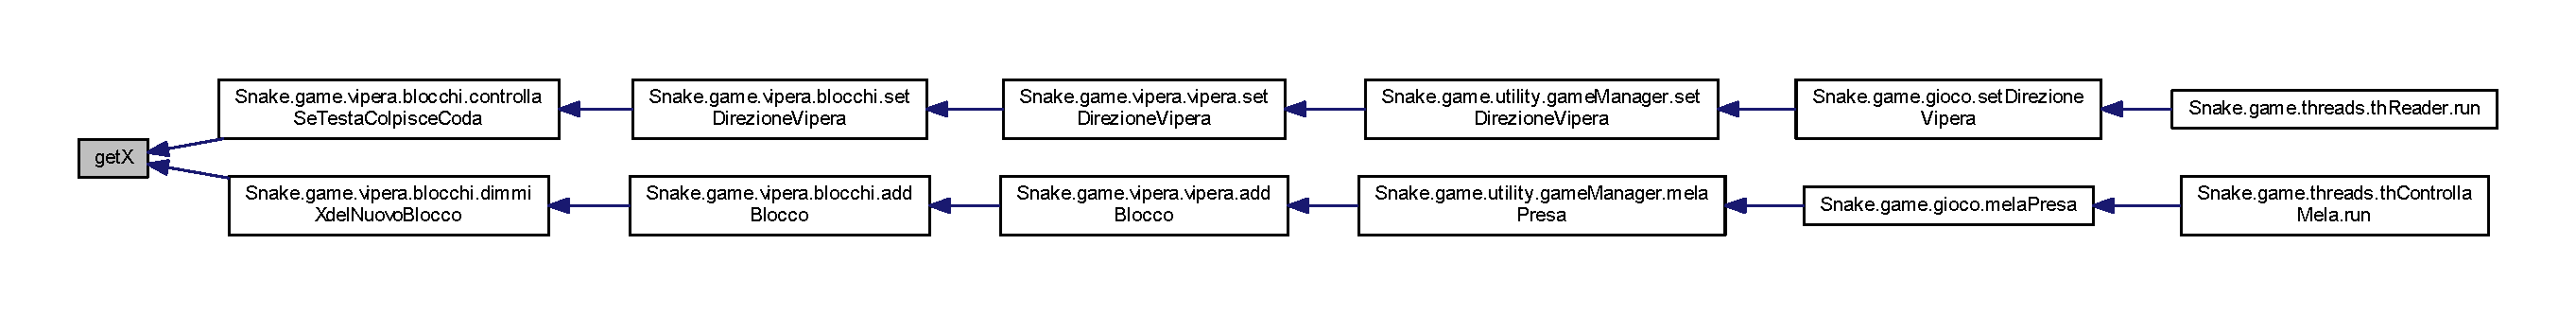
\includegraphics[width=350pt]{class_snake_1_1game_1_1vipera_1_1blocco_ae13f88e922e1339355456062ad9fa359_icgraph}
\end{center}
\end{figure}
\mbox{\Hypertarget{class_snake_1_1game_1_1vipera_1_1blocco_aab81944f0a14bba932c0931899951937}\label{class_snake_1_1game_1_1vipera_1_1blocco_aab81944f0a14bba932c0931899951937}} 
\index{Snake\+::game\+::vipera\+::blocco@{Snake\+::game\+::vipera\+::blocco}!getY@{getY}}
\index{getY@{getY}!Snake\+::game\+::vipera\+::blocco@{Snake\+::game\+::vipera\+::blocco}}
\subsubsection{\texorpdfstring{get\+Y()}{getY()}}
{\footnotesize\ttfamily int getY (\begin{DoxyParamCaption}{ }\end{DoxyParamCaption})}



Ritorna la posizione Y del blocco. 



Definition at line 101 of file blocco.\+java.

Here is the caller graph for this function\+:
\nopagebreak
\begin{figure}[H]
\begin{center}
\leavevmode
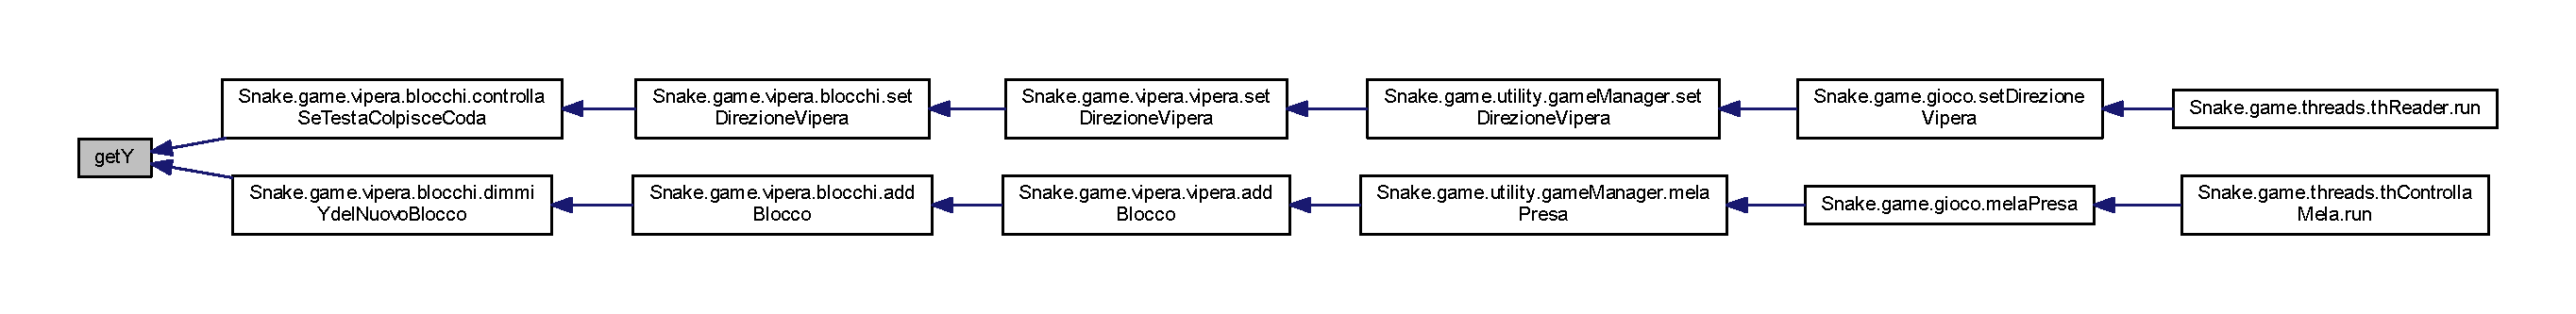
\includegraphics[width=350pt]{class_snake_1_1game_1_1vipera_1_1blocco_aab81944f0a14bba932c0931899951937_icgraph}
\end{center}
\end{figure}
\mbox{\Hypertarget{class_snake_1_1game_1_1vipera_1_1blocco_acabc02ee9509cd1e196033348dd76a6f}\label{class_snake_1_1game_1_1vipera_1_1blocco_acabc02ee9509cd1e196033348dd76a6f}} 
\index{Snake\+::game\+::vipera\+::blocco@{Snake\+::game\+::vipera\+::blocco}!segui@{segui}}
\index{segui@{segui}!Snake\+::game\+::vipera\+::blocco@{Snake\+::game\+::vipera\+::blocco}}
\subsubsection{\texorpdfstring{segui()}{segui()}}
{\footnotesize\ttfamily void segui (\begin{DoxyParamCaption}\item[{\mbox{\hyperlink{enum_snake_1_1game_1_1utility_1_1_directions}{Directions}}}]{dove\+Vado }\end{DoxyParamCaption})}



Il metodo permette di far muovere il blocco a seconda della direzione passata come parametro. 

In base alla dimensione dei blocchi che compongono la vipera viene mosso questo blocco. 

Definition at line 128 of file blocco.\+java.

Here is the call graph for this function\+:
\nopagebreak
\begin{figure}[H]
\begin{center}
\leavevmode
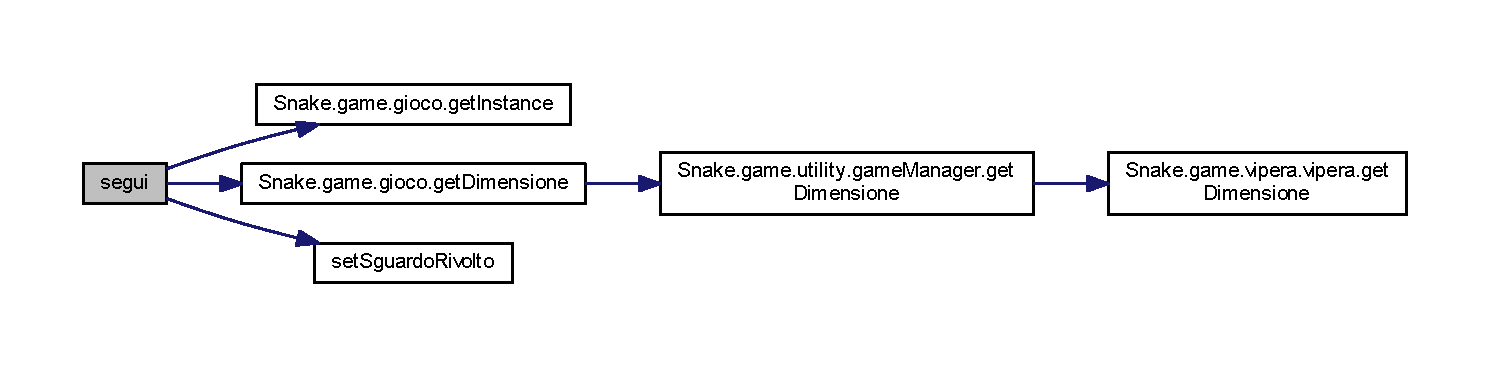
\includegraphics[width=350pt]{class_snake_1_1game_1_1vipera_1_1blocco_acabc02ee9509cd1e196033348dd76a6f_cgraph}
\end{center}
\end{figure}
Here is the caller graph for this function\+:
\nopagebreak
\begin{figure}[H]
\begin{center}
\leavevmode
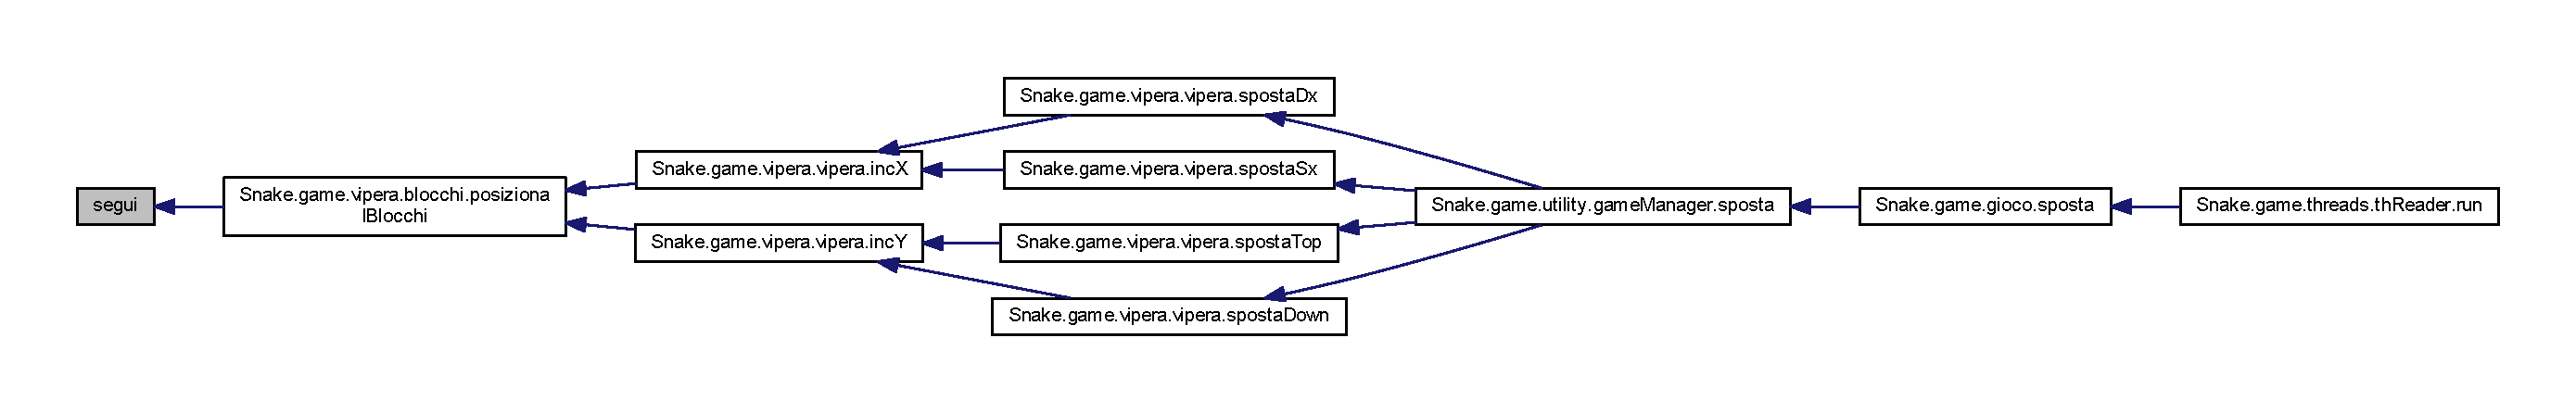
\includegraphics[width=350pt]{class_snake_1_1game_1_1vipera_1_1blocco_acabc02ee9509cd1e196033348dd76a6f_icgraph}
\end{center}
\end{figure}
\mbox{\Hypertarget{class_snake_1_1game_1_1vipera_1_1blocco_a2d20c8ebc9efc39ed12392e6486d50d9}\label{class_snake_1_1game_1_1vipera_1_1blocco_a2d20c8ebc9efc39ed12392e6486d50d9}} 
\index{Snake\+::game\+::vipera\+::blocco@{Snake\+::game\+::vipera\+::blocco}!set\+Sguardo\+Rivolto@{set\+Sguardo\+Rivolto}}
\index{set\+Sguardo\+Rivolto@{set\+Sguardo\+Rivolto}!Snake\+::game\+::vipera\+::blocco@{Snake\+::game\+::vipera\+::blocco}}
\subsubsection{\texorpdfstring{set\+Sguardo\+Rivolto()}{setSguardoRivolto()}}
{\footnotesize\ttfamily void set\+Sguardo\+Rivolto (\begin{DoxyParamCaption}\item[{\mbox{\hyperlink{enum_snake_1_1game_1_1utility_1_1_directions}{Directions}}}]{dir }\end{DoxyParamCaption})}



Il metodo permette di aggiornare l\textquotesingle{}attributo tutte\+Mosse a seconda della direzione passata come parametro. 

Il metodo aggiorna l\textquotesingle{}attributo tutte\+Mosse in modo tale da consentire ai blocchi adiacenti di far seguire la strada che questo blocco ha effettuato (effetto snake). Si preoccupa inoltre della gestione di un altro blocco generato in sua corrispondenza per evitare che venga segnalato come morte (serpente che si mangia la coda) 

Definition at line 72 of file blocco.\+java.

Here is the caller graph for this function\+:
\nopagebreak
\begin{figure}[H]
\begin{center}
\leavevmode
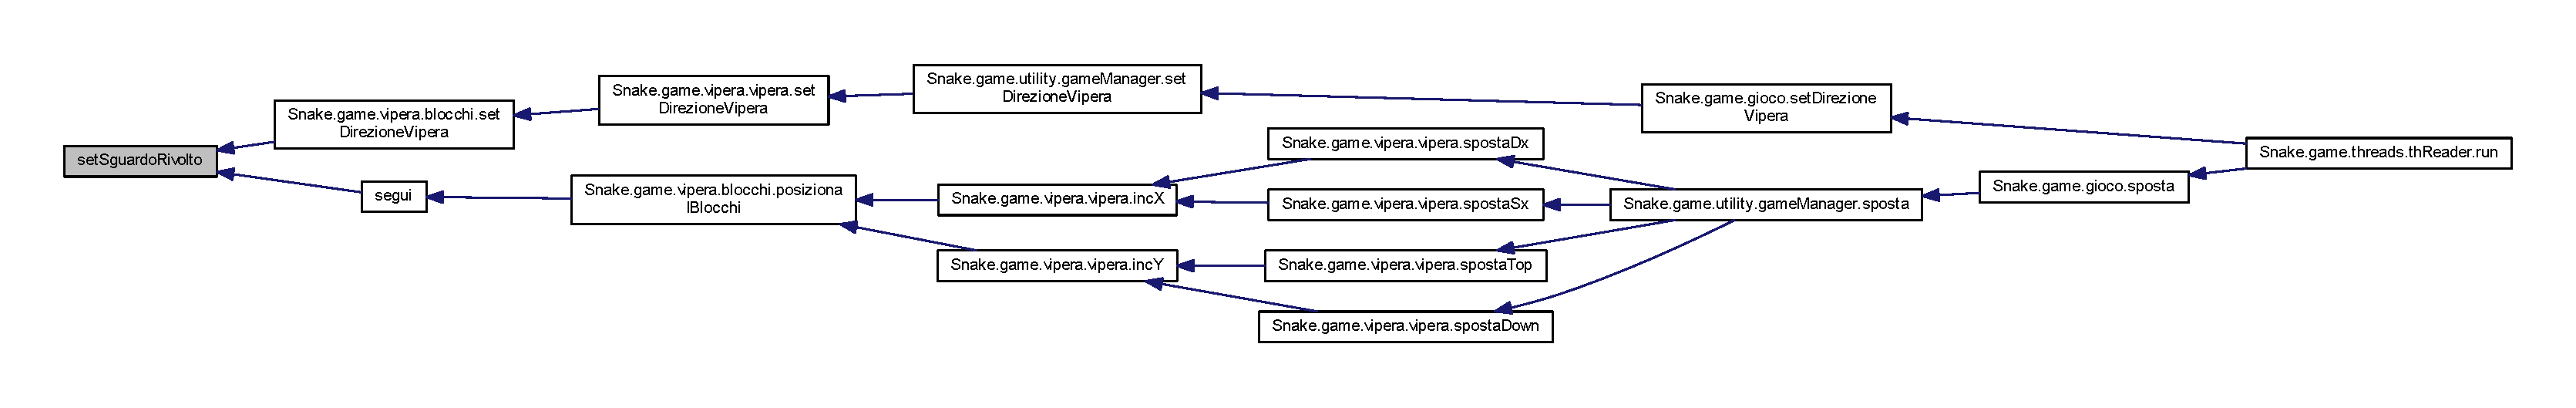
\includegraphics[width=350pt]{class_snake_1_1game_1_1vipera_1_1blocco_a2d20c8ebc9efc39ed12392e6486d50d9_icgraph}
\end{center}
\end{figure}
\mbox{\Hypertarget{class_snake_1_1game_1_1vipera_1_1blocco_ab5a3acb0391238ee37a5da898bffd5f1}\label{class_snake_1_1game_1_1vipera_1_1blocco_ab5a3acb0391238ee37a5da898bffd5f1}} 
\index{Snake\+::game\+::vipera\+::blocco@{Snake\+::game\+::vipera\+::blocco}!setX@{setX}}
\index{setX@{setX}!Snake\+::game\+::vipera\+::blocco@{Snake\+::game\+::vipera\+::blocco}}
\subsubsection{\texorpdfstring{set\+X()}{setX()}}
{\footnotesize\ttfamily void setX (\begin{DoxyParamCaption}\item[{int}]{act\+PosX }\end{DoxyParamCaption})}



Imposta la posizione X del blocco a seconda del parametro. 


\begin{DoxyParams}{Parameters}
{\em act\+PosX} & posizioneX \\
\hline
\end{DoxyParams}


Definition at line 110 of file blocco.\+java.

Here is the caller graph for this function\+:
\nopagebreak
\begin{figure}[H]
\begin{center}
\leavevmode
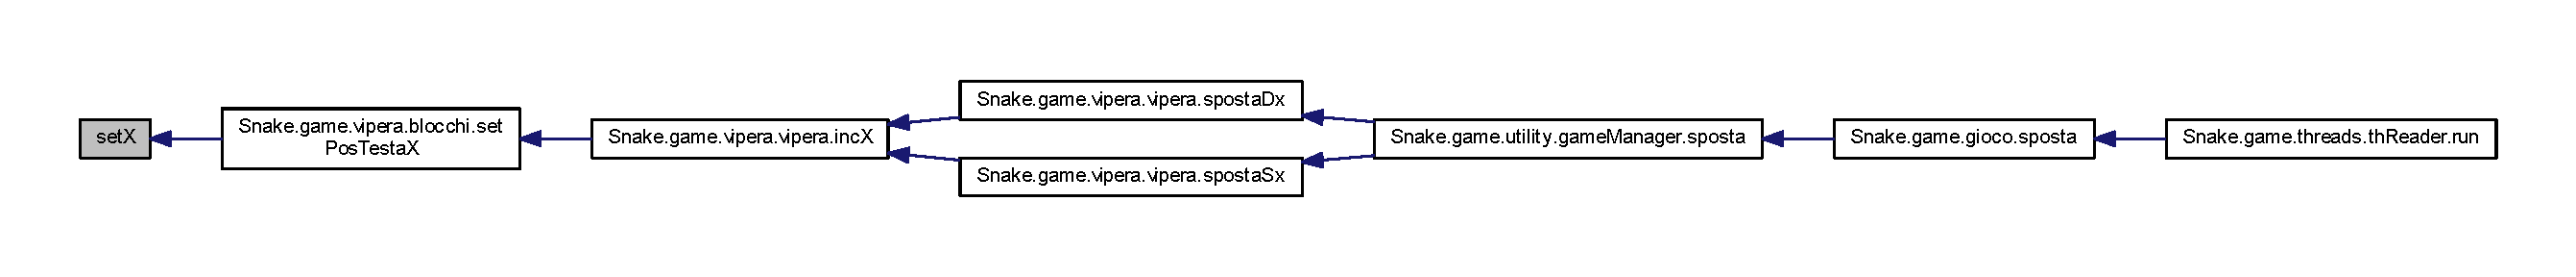
\includegraphics[width=350pt]{class_snake_1_1game_1_1vipera_1_1blocco_ab5a3acb0391238ee37a5da898bffd5f1_icgraph}
\end{center}
\end{figure}
\mbox{\Hypertarget{class_snake_1_1game_1_1vipera_1_1blocco_a60e970e880a18799c14e771afe3e904b}\label{class_snake_1_1game_1_1vipera_1_1blocco_a60e970e880a18799c14e771afe3e904b}} 
\index{Snake\+::game\+::vipera\+::blocco@{Snake\+::game\+::vipera\+::blocco}!setY@{setY}}
\index{setY@{setY}!Snake\+::game\+::vipera\+::blocco@{Snake\+::game\+::vipera\+::blocco}}
\subsubsection{\texorpdfstring{set\+Y()}{setY()}}
{\footnotesize\ttfamily void setY (\begin{DoxyParamCaption}\item[{int}]{act\+PosY }\end{DoxyParamCaption})}



Imposta la posizione Y del blocco a seconda del parametro. 


\begin{DoxyParams}{Parameters}
{\em act\+PosY} & posizioneY \\
\hline
\end{DoxyParams}


Definition at line 118 of file blocco.\+java.

Here is the caller graph for this function\+:
\nopagebreak
\begin{figure}[H]
\begin{center}
\leavevmode
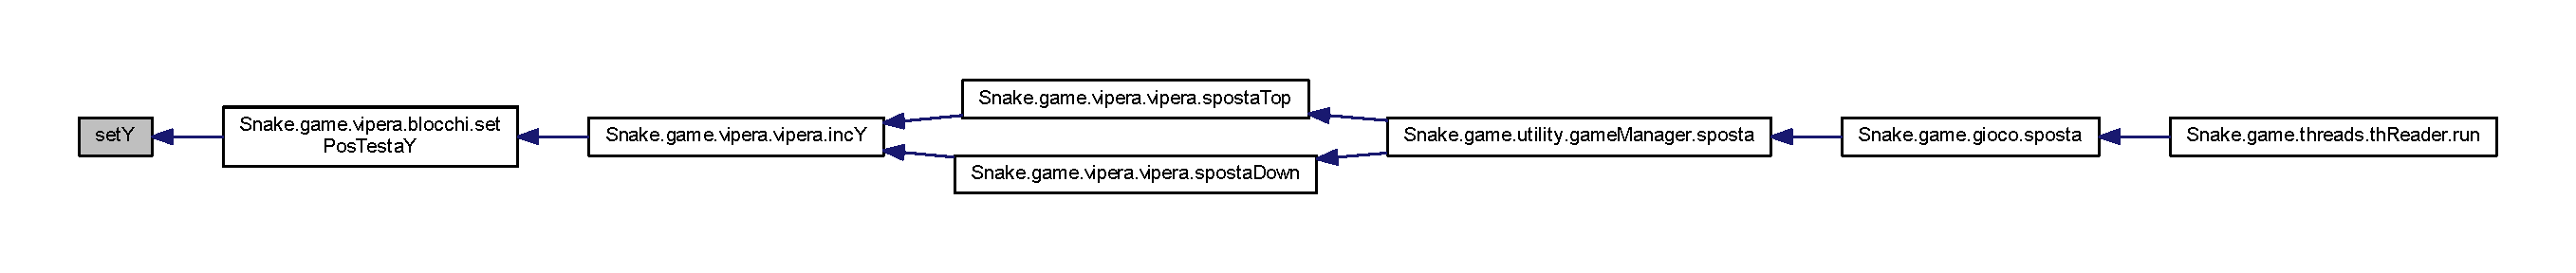
\includegraphics[width=350pt]{class_snake_1_1game_1_1vipera_1_1blocco_a60e970e880a18799c14e771afe3e904b_icgraph}
\end{center}
\end{figure}


\subsection{Member Data Documentation}
\mbox{\Hypertarget{class_snake_1_1game_1_1vipera_1_1blocco_aaa64105e6cedf2b98a63e3ab8c8f4cdb}\label{class_snake_1_1game_1_1vipera_1_1blocco_aaa64105e6cedf2b98a63e3ab8c8f4cdb}} 
\index{Snake\+::game\+::vipera\+::blocco@{Snake\+::game\+::vipera\+::blocco}!act\+PosX@{act\+PosX}}
\index{act\+PosX@{act\+PosX}!Snake\+::game\+::vipera\+::blocco@{Snake\+::game\+::vipera\+::blocco}}
\subsubsection{\texorpdfstring{act\+PosX}{actPosX}}
{\footnotesize\ttfamily int act\+PosX\hspace{0.3cm}{\ttfamily [private]}}

Attributo che rappresenta la posizione X del blocco 

Definition at line 17 of file blocco.\+java.

\mbox{\Hypertarget{class_snake_1_1game_1_1vipera_1_1blocco_a301b22c6bff25f4530e3f991788338fe}\label{class_snake_1_1game_1_1vipera_1_1blocco_a301b22c6bff25f4530e3f991788338fe}} 
\index{Snake\+::game\+::vipera\+::blocco@{Snake\+::game\+::vipera\+::blocco}!act\+PosY@{act\+PosY}}
\index{act\+PosY@{act\+PosY}!Snake\+::game\+::vipera\+::blocco@{Snake\+::game\+::vipera\+::blocco}}
\subsubsection{\texorpdfstring{act\+PosY}{actPosY}}
{\footnotesize\ttfamily int act\+PosY\hspace{0.3cm}{\ttfamily [private]}}

Attributo che rappresenta la posizione Y del blocco 

Definition at line 19 of file blocco.\+java.

\mbox{\Hypertarget{class_snake_1_1game_1_1vipera_1_1blocco_ada0bf0be39e4ad9d58f6e7c48f14c64a}\label{class_snake_1_1game_1_1vipera_1_1blocco_ada0bf0be39e4ad9d58f6e7c48f14c64a}} 
\index{Snake\+::game\+::vipera\+::blocco@{Snake\+::game\+::vipera\+::blocco}!colore@{colore}}
\index{colore@{colore}!Snake\+::game\+::vipera\+::blocco@{Snake\+::game\+::vipera\+::blocco}}
\subsubsection{\texorpdfstring{colore}{colore}}
{\footnotesize\ttfamily Color colore\hspace{0.3cm}{\ttfamily [private]}}

Attributo che rappresenta il colore del blocco 

Definition at line 31 of file blocco.\+java.

\mbox{\Hypertarget{class_snake_1_1game_1_1vipera_1_1blocco_aab706c0c0218d17f9386c9dce8989195}\label{class_snake_1_1game_1_1vipera_1_1blocco_aab706c0c0218d17f9386c9dce8989195}} 
\index{Snake\+::game\+::vipera\+::blocco@{Snake\+::game\+::vipera\+::blocco}!distacca\+Figlio@{distacca\+Figlio}}
\index{distacca\+Figlio@{distacca\+Figlio}!Snake\+::game\+::vipera\+::blocco@{Snake\+::game\+::vipera\+::blocco}}
\subsubsection{\texorpdfstring{distacca\+Figlio}{distaccaFiglio}}
{\footnotesize\ttfamily boolean distacca\+Figlio\hspace{0.3cm}{\ttfamily [private]}}

Attributo che afferma se si e\textquotesingle{} distaccato il blocco in corrispondenza di almeno un unita\textquotesingle{} 

Definition at line 28 of file blocco.\+java.

\mbox{\Hypertarget{class_snake_1_1game_1_1vipera_1_1blocco_a909ed9e20b51021224373cb7e95365e7}\label{class_snake_1_1game_1_1vipera_1_1blocco_a909ed9e20b51021224373cb7e95365e7}} 
\index{Snake\+::game\+::vipera\+::blocco@{Snake\+::game\+::vipera\+::blocco}!ho\+Un\+Figlio@{ho\+Un\+Figlio}}
\index{ho\+Un\+Figlio@{ho\+Un\+Figlio}!Snake\+::game\+::vipera\+::blocco@{Snake\+::game\+::vipera\+::blocco}}
\subsubsection{\texorpdfstring{ho\+Un\+Figlio}{hoUnFiglio}}
{\footnotesize\ttfamily boolean ho\+Un\+Figlio\hspace{0.3cm}{\ttfamily [private]}}

Attributo che se true significa che un altro blocco e\textquotesingle{} stato generato in corrispondenza di questo blocco 

Definition at line 25 of file blocco.\+java.

\mbox{\Hypertarget{class_snake_1_1game_1_1vipera_1_1blocco_a0670f48287135d82c64441e965d35c18}\label{class_snake_1_1game_1_1vipera_1_1blocco_a0670f48287135d82c64441e965d35c18}} 
\index{Snake\+::game\+::vipera\+::blocco@{Snake\+::game\+::vipera\+::blocco}!tutte\+Mosse@{tutte\+Mosse}}
\index{tutte\+Mosse@{tutte\+Mosse}!Snake\+::game\+::vipera\+::blocco@{Snake\+::game\+::vipera\+::blocco}}
\subsubsection{\texorpdfstring{tutte\+Mosse}{tutteMosse}}
{\footnotesize\ttfamily Vector$<$\mbox{\hyperlink{enum_snake_1_1game_1_1utility_1_1_directions}{Directions}}$>$ tutte\+Mosse = new Vector$<$\mbox{\hyperlink{enum_snake_1_1game_1_1utility_1_1_directions}{Directions}}$>$()\hspace{0.3cm}{\ttfamily [private]}}

Attributo che corrisponde alle mosse effettuate dal blocco 

Definition at line 22 of file blocco.\+java.



The documentation for this class was generated from the following file\+:\begin{DoxyCompactItemize}
\item 
src/main/java/\+Snake/game/vipera/\mbox{\hyperlink{blocco_8java}{blocco.\+java}}\end{DoxyCompactItemize}

\hypertarget{class_snake_1_1game_1_1utility_1_1commands}{}\section{commands Class Reference}
\label{class_snake_1_1game_1_1utility_1_1commands}\index{commands@{commands}}


Collaboration diagram for commands\+:
\nopagebreak
\begin{figure}[H]
\begin{center}
\leavevmode
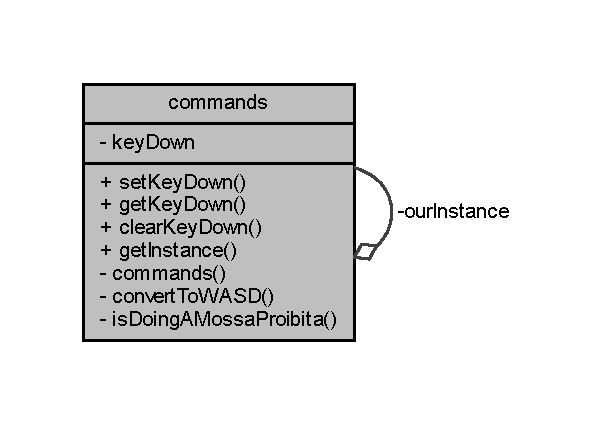
\includegraphics[width=285pt]{class_snake_1_1game_1_1utility_1_1commands__coll__graph}
\end{center}
\end{figure}
\subsection*{Public Member Functions}
\begin{DoxyCompactItemize}
\item 
void \mbox{\hyperlink{class_snake_1_1game_1_1utility_1_1commands_a116fb077976b2f81b0fc36845423fadb}{set\+Key\+Down}} (Character car, int key\+Code)
\begin{DoxyCompactList}\small\item\em Il metodo permette di impostare l\textquotesingle{}attributo key\+Down in base ai parametri passati. \end{DoxyCompactList}\item 
Character \mbox{\hyperlink{class_snake_1_1game_1_1utility_1_1commands_aca1e2aeb7fb5a02cf6127edc96edc7f6}{get\+Key\+Down}} ()
\begin{DoxyCompactList}\small\item\em Ritorna l\textquotesingle{}ultimo comando inviato (key\+Down) \end{DoxyCompactList}\item 
void \mbox{\hyperlink{class_snake_1_1game_1_1utility_1_1commands_a8b2e8ab4e21c2a33e48e38fb8567fb19}{clear\+Key\+Down}} ()
\begin{DoxyCompactList}\small\item\em Resetta l\textquotesingle{}attributo key\+Down. \end{DoxyCompactList}\end{DoxyCompactItemize}
\subsection*{Static Public Member Functions}
\begin{DoxyCompactItemize}
\item 
static \mbox{\hyperlink{class_snake_1_1game_1_1utility_1_1commands}{commands}} \mbox{\hyperlink{class_snake_1_1game_1_1utility_1_1commands_a388ff71d8b8e9c6f6a68839aa5575acc}{get\+Instance}} ()
\end{DoxyCompactItemize}
\subsection*{Private Member Functions}
\begin{DoxyCompactItemize}
\item 
\mbox{\hyperlink{class_snake_1_1game_1_1utility_1_1commands_af0afefa0d79d09344a638cf6c532aa39}{commands}} ()
\begin{DoxyCompactList}\small\item\em Costruttore privato senza parametri della classe. \end{DoxyCompactList}\item 
Character \mbox{\hyperlink{class_snake_1_1game_1_1utility_1_1commands_a66de6f4fd0fc79b7d17dc3196aa5fe7e}{convert\+To\+W\+A\+SD}} (int key\+Code)
\begin{DoxyCompactList}\small\item\em Il metodo converte il parametro passato nella sequenza di tasti W\+A\+SD. \end{DoxyCompactList}\item 
boolean \mbox{\hyperlink{class_snake_1_1game_1_1utility_1_1commands_a5852b0c61e12c9a0dff32d89faf56a0f}{is\+Doing\+A\+Mossa\+Proibita}} (Character car)
\begin{DoxyCompactList}\small\item\em Metodo che ritorna true quando vogliamo tornare indietro sullo stesso asse. \end{DoxyCompactList}\end{DoxyCompactItemize}
\subsection*{Private Attributes}
\begin{DoxyCompactItemize}
\item 
Character \mbox{\hyperlink{class_snake_1_1game_1_1utility_1_1commands_a09bac1b4079089c0f6a6eff874a820b8}{key\+Down}}
\end{DoxyCompactItemize}
\subsection*{Static Private Attributes}
\begin{DoxyCompactItemize}
\item 
static \mbox{\hyperlink{class_snake_1_1game_1_1utility_1_1commands}{commands}} \mbox{\hyperlink{class_snake_1_1game_1_1utility_1_1commands_aa7a70ebde8ae359567827667a6ce1901}{our\+Instance}} = new \mbox{\hyperlink{class_snake_1_1game_1_1utility_1_1commands}{commands}}()
\end{DoxyCompactItemize}


\subsection{Detailed Description}
\begin{DoxyAuthor}{Author}
Saccani Federico, \href{mailto:federico.saccani01@gmail.com}{\tt federico.\+saccani01@gmail.\+com} 
\end{DoxyAuthor}
\begin{DoxyVersion}{Version}
1.\+0 ~\newline
La classe gestisce i comandi inviati da tastiera 
\end{DoxyVersion}


Definition at line 15 of file commands.\+java.



\subsection{Constructor \& Destructor Documentation}
\mbox{\Hypertarget{class_snake_1_1game_1_1utility_1_1commands_af0afefa0d79d09344a638cf6c532aa39}\label{class_snake_1_1game_1_1utility_1_1commands_af0afefa0d79d09344a638cf6c532aa39}} 
\index{Snake\+::game\+::utility\+::commands@{Snake\+::game\+::utility\+::commands}!commands@{commands}}
\index{commands@{commands}!Snake\+::game\+::utility\+::commands@{Snake\+::game\+::utility\+::commands}}
\subsubsection{\texorpdfstring{commands()}{commands()}}
{\footnotesize\ttfamily \mbox{\hyperlink{class_snake_1_1game_1_1utility_1_1commands}{commands}} (\begin{DoxyParamCaption}{ }\end{DoxyParamCaption})\hspace{0.3cm}{\ttfamily [private]}}



Costruttore privato senza parametri della classe. 



Definition at line 28 of file commands.\+java.



\subsection{Member Function Documentation}
\mbox{\Hypertarget{class_snake_1_1game_1_1utility_1_1commands_a8b2e8ab4e21c2a33e48e38fb8567fb19}\label{class_snake_1_1game_1_1utility_1_1commands_a8b2e8ab4e21c2a33e48e38fb8567fb19}} 
\index{Snake\+::game\+::utility\+::commands@{Snake\+::game\+::utility\+::commands}!clear\+Key\+Down@{clear\+Key\+Down}}
\index{clear\+Key\+Down@{clear\+Key\+Down}!Snake\+::game\+::utility\+::commands@{Snake\+::game\+::utility\+::commands}}
\subsubsection{\texorpdfstring{clear\+Key\+Down()}{clearKeyDown()}}
{\footnotesize\ttfamily void clear\+Key\+Down (\begin{DoxyParamCaption}{ }\end{DoxyParamCaption})}



Resetta l\textquotesingle{}attributo key\+Down. 



Definition at line 66 of file commands.\+java.

Here is the caller graph for this function\+:
\nopagebreak
\begin{figure}[H]
\begin{center}
\leavevmode
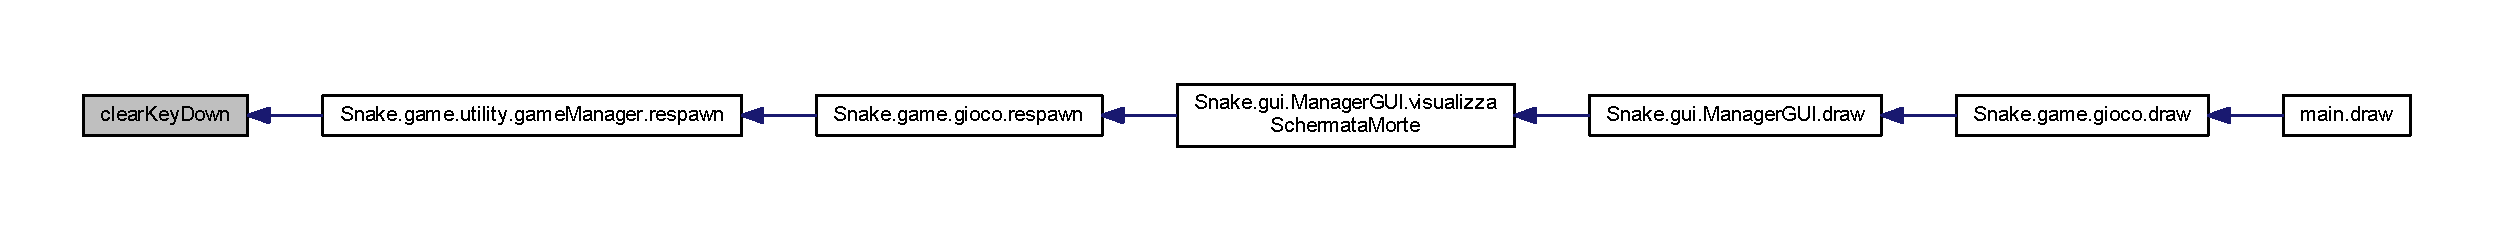
\includegraphics[width=350pt]{class_snake_1_1game_1_1utility_1_1commands_a8b2e8ab4e21c2a33e48e38fb8567fb19_icgraph}
\end{center}
\end{figure}
\mbox{\Hypertarget{class_snake_1_1game_1_1utility_1_1commands_a66de6f4fd0fc79b7d17dc3196aa5fe7e}\label{class_snake_1_1game_1_1utility_1_1commands_a66de6f4fd0fc79b7d17dc3196aa5fe7e}} 
\index{Snake\+::game\+::utility\+::commands@{Snake\+::game\+::utility\+::commands}!convert\+To\+W\+A\+SD@{convert\+To\+W\+A\+SD}}
\index{convert\+To\+W\+A\+SD@{convert\+To\+W\+A\+SD}!Snake\+::game\+::utility\+::commands@{Snake\+::game\+::utility\+::commands}}
\subsubsection{\texorpdfstring{convert\+To\+W\+A\+S\+D()}{convertToWASD()}}
{\footnotesize\ttfamily Character convert\+To\+W\+A\+SD (\begin{DoxyParamCaption}\item[{int}]{key\+Code }\end{DoxyParamCaption})\hspace{0.3cm}{\ttfamily [private]}}



Il metodo converte il parametro passato nella sequenza di tasti W\+A\+SD. 


\begin{DoxyParams}{Parameters}
{\em key\+Code} & codice del tasto riferito alle frecce della tastiera che deve essere trasformato in W\+A\+SD \\
\hline
\end{DoxyParams}


Definition at line 75 of file commands.\+java.

Here is the caller graph for this function\+:
\nopagebreak
\begin{figure}[H]
\begin{center}
\leavevmode
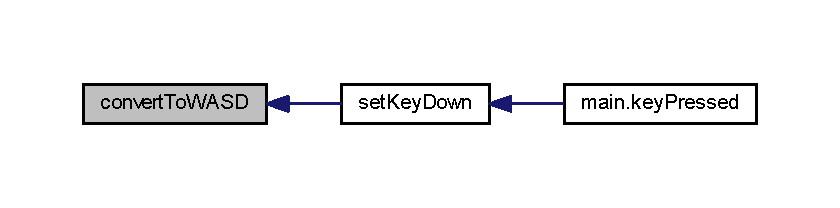
\includegraphics[width=350pt]{class_snake_1_1game_1_1utility_1_1commands_a66de6f4fd0fc79b7d17dc3196aa5fe7e_icgraph}
\end{center}
\end{figure}
\mbox{\Hypertarget{class_snake_1_1game_1_1utility_1_1commands_a388ff71d8b8e9c6f6a68839aa5575acc}\label{class_snake_1_1game_1_1utility_1_1commands_a388ff71d8b8e9c6f6a68839aa5575acc}} 
\index{Snake\+::game\+::utility\+::commands@{Snake\+::game\+::utility\+::commands}!get\+Instance@{get\+Instance}}
\index{get\+Instance@{get\+Instance}!Snake\+::game\+::utility\+::commands@{Snake\+::game\+::utility\+::commands}}
\subsubsection{\texorpdfstring{get\+Instance()}{getInstance()}}
{\footnotesize\ttfamily static \mbox{\hyperlink{class_snake_1_1game_1_1utility_1_1commands}{commands}} get\+Instance (\begin{DoxyParamCaption}{ }\end{DoxyParamCaption})\hspace{0.3cm}{\ttfamily [static]}}

Attributo che rappresenta l\textquotesingle{}instance pubblica per singleton 

Definition at line 21 of file commands.\+java.

Here is the caller graph for this function\+:
\nopagebreak
\begin{figure}[H]
\begin{center}
\leavevmode
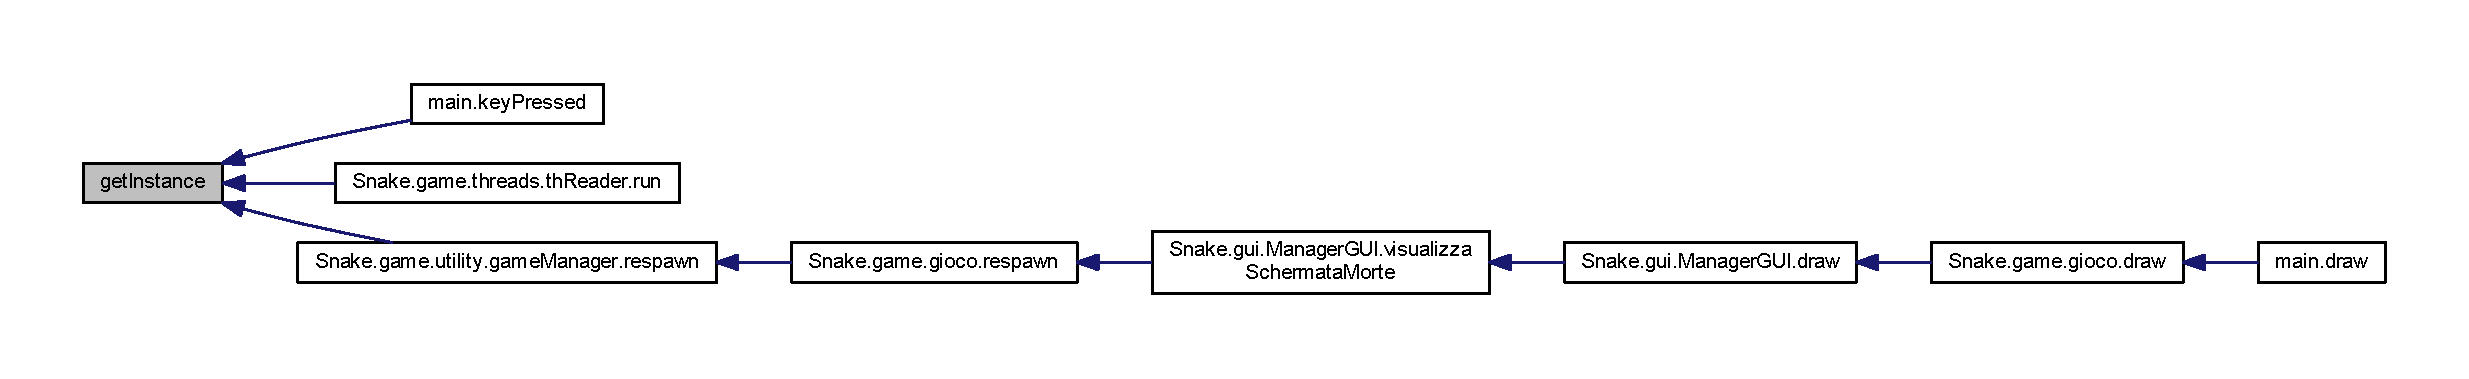
\includegraphics[width=350pt]{class_snake_1_1game_1_1utility_1_1commands_a388ff71d8b8e9c6f6a68839aa5575acc_icgraph}
\end{center}
\end{figure}
\mbox{\Hypertarget{class_snake_1_1game_1_1utility_1_1commands_aca1e2aeb7fb5a02cf6127edc96edc7f6}\label{class_snake_1_1game_1_1utility_1_1commands_aca1e2aeb7fb5a02cf6127edc96edc7f6}} 
\index{Snake\+::game\+::utility\+::commands@{Snake\+::game\+::utility\+::commands}!get\+Key\+Down@{get\+Key\+Down}}
\index{get\+Key\+Down@{get\+Key\+Down}!Snake\+::game\+::utility\+::commands@{Snake\+::game\+::utility\+::commands}}
\subsubsection{\texorpdfstring{get\+Key\+Down()}{getKeyDown()}}
{\footnotesize\ttfamily Character get\+Key\+Down (\begin{DoxyParamCaption}{ }\end{DoxyParamCaption})}



Ritorna l\textquotesingle{}ultimo comando inviato (key\+Down) 



Definition at line 59 of file commands.\+java.

Here is the caller graph for this function\+:
\nopagebreak
\begin{figure}[H]
\begin{center}
\leavevmode
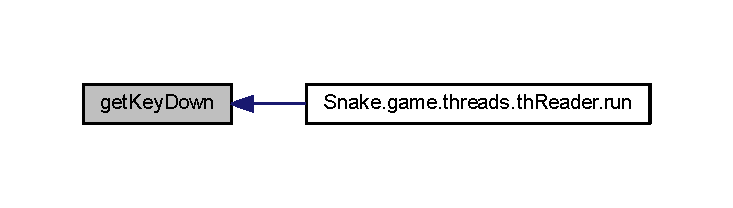
\includegraphics[width=350pt]{class_snake_1_1game_1_1utility_1_1commands_aca1e2aeb7fb5a02cf6127edc96edc7f6_icgraph}
\end{center}
\end{figure}
\mbox{\Hypertarget{class_snake_1_1game_1_1utility_1_1commands_a5852b0c61e12c9a0dff32d89faf56a0f}\label{class_snake_1_1game_1_1utility_1_1commands_a5852b0c61e12c9a0dff32d89faf56a0f}} 
\index{Snake\+::game\+::utility\+::commands@{Snake\+::game\+::utility\+::commands}!is\+Doing\+A\+Mossa\+Proibita@{is\+Doing\+A\+Mossa\+Proibita}}
\index{is\+Doing\+A\+Mossa\+Proibita@{is\+Doing\+A\+Mossa\+Proibita}!Snake\+::game\+::utility\+::commands@{Snake\+::game\+::utility\+::commands}}
\subsubsection{\texorpdfstring{is\+Doing\+A\+Mossa\+Proibita()}{isDoingAMossaProibita()}}
{\footnotesize\ttfamily boolean is\+Doing\+A\+Mossa\+Proibita (\begin{DoxyParamCaption}\item[{Character}]{car }\end{DoxyParamCaption})\hspace{0.3cm}{\ttfamily [private]}}



Metodo che ritorna true quando vogliamo tornare indietro sullo stesso asse. 

Evita che vengano eseguiti comandi di cambio direzione sullo stesso asse. Esempio\+: mi sto muovendo a DX, non posso dire di muovermi a SX perche\textquotesingle{} altrimenti andrei a sovrappormi con la testa sulla coda 

Definition at line 106 of file commands.\+java.

Here is the caller graph for this function\+:
\nopagebreak
\begin{figure}[H]
\begin{center}
\leavevmode
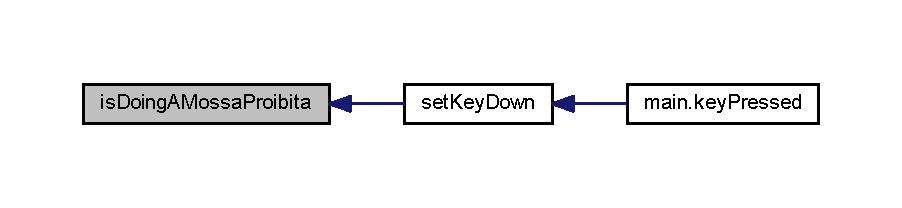
\includegraphics[width=350pt]{class_snake_1_1game_1_1utility_1_1commands_a5852b0c61e12c9a0dff32d89faf56a0f_icgraph}
\end{center}
\end{figure}
\mbox{\Hypertarget{class_snake_1_1game_1_1utility_1_1commands_a116fb077976b2f81b0fc36845423fadb}\label{class_snake_1_1game_1_1utility_1_1commands_a116fb077976b2f81b0fc36845423fadb}} 
\index{Snake\+::game\+::utility\+::commands@{Snake\+::game\+::utility\+::commands}!set\+Key\+Down@{set\+Key\+Down}}
\index{set\+Key\+Down@{set\+Key\+Down}!Snake\+::game\+::utility\+::commands@{Snake\+::game\+::utility\+::commands}}
\subsubsection{\texorpdfstring{set\+Key\+Down()}{setKeyDown()}}
{\footnotesize\ttfamily void set\+Key\+Down (\begin{DoxyParamCaption}\item[{Character}]{car,  }\item[{int}]{key\+Code }\end{DoxyParamCaption})}



Il metodo permette di impostare l\textquotesingle{}attributo key\+Down in base ai parametri passati. 

Il metodo converte l\textquotesingle{}input delle frecce della tastiera nei rispettivi comandi W\+A\+SD 
\begin{DoxyParams}{Parameters}
{\em car} & carattere premuto su tastiera \\
\hline
{\em key\+Code} & codice del carattere premuto su tastiera \\
\hline
\end{DoxyParams}


Definition at line 39 of file commands.\+java.

Here is the call graph for this function\+:
\nopagebreak
\begin{figure}[H]
\begin{center}
\leavevmode
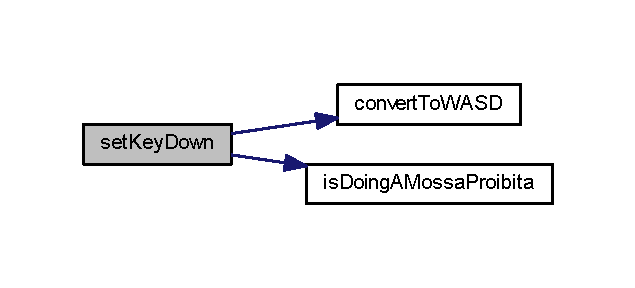
\includegraphics[width=305pt]{class_snake_1_1game_1_1utility_1_1commands_a116fb077976b2f81b0fc36845423fadb_cgraph}
\end{center}
\end{figure}
Here is the caller graph for this function\+:
\nopagebreak
\begin{figure}[H]
\begin{center}
\leavevmode
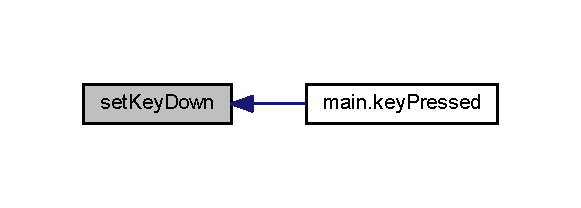
\includegraphics[width=279pt]{class_snake_1_1game_1_1utility_1_1commands_a116fb077976b2f81b0fc36845423fadb_icgraph}
\end{center}
\end{figure}


\subsection{Member Data Documentation}
\mbox{\Hypertarget{class_snake_1_1game_1_1utility_1_1commands_a09bac1b4079089c0f6a6eff874a820b8}\label{class_snake_1_1game_1_1utility_1_1commands_a09bac1b4079089c0f6a6eff874a820b8}} 
\index{Snake\+::game\+::utility\+::commands@{Snake\+::game\+::utility\+::commands}!key\+Down@{key\+Down}}
\index{key\+Down@{key\+Down}!Snake\+::game\+::utility\+::commands@{Snake\+::game\+::utility\+::commands}}
\subsubsection{\texorpdfstring{key\+Down}{keyDown}}
{\footnotesize\ttfamily Character key\+Down\hspace{0.3cm}{\ttfamily [private]}}

Attributo che rappresenta l\textquotesingle{}ultimo comando inviato 

Definition at line 17 of file commands.\+java.

\mbox{\Hypertarget{class_snake_1_1game_1_1utility_1_1commands_aa7a70ebde8ae359567827667a6ce1901}\label{class_snake_1_1game_1_1utility_1_1commands_aa7a70ebde8ae359567827667a6ce1901}} 
\index{Snake\+::game\+::utility\+::commands@{Snake\+::game\+::utility\+::commands}!our\+Instance@{our\+Instance}}
\index{our\+Instance@{our\+Instance}!Snake\+::game\+::utility\+::commands@{Snake\+::game\+::utility\+::commands}}
\subsubsection{\texorpdfstring{our\+Instance}{ourInstance}}
{\footnotesize\ttfamily \mbox{\hyperlink{class_snake_1_1game_1_1utility_1_1commands}{commands}} our\+Instance = new \mbox{\hyperlink{class_snake_1_1game_1_1utility_1_1commands}{commands}}()\hspace{0.3cm}{\ttfamily [static]}, {\ttfamily [private]}}

Attributo che rappresenta l\textquotesingle{}instance privata per singleton 

Definition at line 19 of file commands.\+java.



The documentation for this class was generated from the following file\+:\begin{DoxyCompactItemize}
\item 
src/main/java/\+Snake/game/utility/\mbox{\hyperlink{commands_8java}{commands.\+java}}\end{DoxyCompactItemize}

\hypertarget{enum_snake_1_1game_1_1utility_1_1_directions}{}\section{Directions Enum Reference}
\label{enum_snake_1_1game_1_1utility_1_1_directions}\index{Directions@{Directions}}


Collaboration diagram for Directions\+:
\nopagebreak
\begin{figure}[H]
\begin{center}
\leavevmode
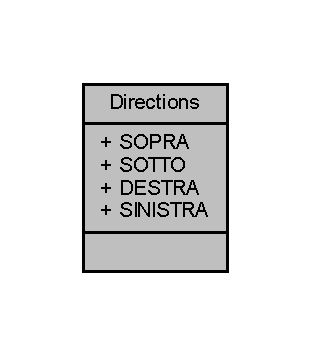
\includegraphics[width=149pt]{enum_snake_1_1game_1_1utility_1_1_directions__coll__graph}
\end{center}
\end{figure}
\subsection*{Public Attributes}
\begin{DoxyCompactItemize}
\item 
\mbox{\hyperlink{enum_snake_1_1game_1_1utility_1_1_directions_a6618b322e7de5b853ac903da736e5dbc}{S\+O\+P\+RA}}
\item 
\mbox{\hyperlink{enum_snake_1_1game_1_1utility_1_1_directions_a6fcef6b13f7f1deeda7fee7cf15280be}{S\+O\+T\+TO}}
\item 
\mbox{\hyperlink{enum_snake_1_1game_1_1utility_1_1_directions_ac15481c77c0c558ceeb3abf2e3b799ab}{D\+E\+S\+T\+RA}}
\item 
\mbox{\hyperlink{enum_snake_1_1game_1_1utility_1_1_directions_aefdfbf72cfaabb51a33d6d9e10add0b5}{S\+I\+N\+I\+S\+T\+RA}}
\end{DoxyCompactItemize}


\subsection{Detailed Description}
\begin{DoxyAuthor}{Author}
Saccani Federico, \href{mailto:federico.saccani01@gmail.com}{\tt federico.\+saccani01@gmail.\+com} 
\end{DoxyAuthor}
\begin{DoxyVersion}{Version}
1.\+0 ~\newline
La classe rappresenta le possibili direzioni che potranno essere effettuate dal serpente 
\end{DoxyVersion}


Definition at line 15 of file Directions.\+java.



\subsection{Member Data Documentation}
\mbox{\Hypertarget{enum_snake_1_1game_1_1utility_1_1_directions_ac15481c77c0c558ceeb3abf2e3b799ab}\label{enum_snake_1_1game_1_1utility_1_1_directions_ac15481c77c0c558ceeb3abf2e3b799ab}} 
\index{Snake\+::game\+::utility\+::\+Directions@{Snake\+::game\+::utility\+::\+Directions}!D\+E\+S\+T\+RA@{D\+E\+S\+T\+RA}}
\index{D\+E\+S\+T\+RA@{D\+E\+S\+T\+RA}!Snake\+::game\+::utility\+::\+Directions@{Snake\+::game\+::utility\+::\+Directions}}
\subsubsection{\texorpdfstring{D\+E\+S\+T\+RA}{DESTRA}}
{\footnotesize\ttfamily D\+E\+S\+T\+RA}



Definition at line 16 of file Directions.\+java.

\mbox{\Hypertarget{enum_snake_1_1game_1_1utility_1_1_directions_aefdfbf72cfaabb51a33d6d9e10add0b5}\label{enum_snake_1_1game_1_1utility_1_1_directions_aefdfbf72cfaabb51a33d6d9e10add0b5}} 
\index{Snake\+::game\+::utility\+::\+Directions@{Snake\+::game\+::utility\+::\+Directions}!S\+I\+N\+I\+S\+T\+RA@{S\+I\+N\+I\+S\+T\+RA}}
\index{S\+I\+N\+I\+S\+T\+RA@{S\+I\+N\+I\+S\+T\+RA}!Snake\+::game\+::utility\+::\+Directions@{Snake\+::game\+::utility\+::\+Directions}}
\subsubsection{\texorpdfstring{S\+I\+N\+I\+S\+T\+RA}{SINISTRA}}
{\footnotesize\ttfamily S\+I\+N\+I\+S\+T\+RA}



Definition at line 16 of file Directions.\+java.

\mbox{\Hypertarget{enum_snake_1_1game_1_1utility_1_1_directions_a6618b322e7de5b853ac903da736e5dbc}\label{enum_snake_1_1game_1_1utility_1_1_directions_a6618b322e7de5b853ac903da736e5dbc}} 
\index{Snake\+::game\+::utility\+::\+Directions@{Snake\+::game\+::utility\+::\+Directions}!S\+O\+P\+RA@{S\+O\+P\+RA}}
\index{S\+O\+P\+RA@{S\+O\+P\+RA}!Snake\+::game\+::utility\+::\+Directions@{Snake\+::game\+::utility\+::\+Directions}}
\subsubsection{\texorpdfstring{S\+O\+P\+RA}{SOPRA}}
{\footnotesize\ttfamily S\+O\+P\+RA}



Definition at line 16 of file Directions.\+java.

\mbox{\Hypertarget{enum_snake_1_1game_1_1utility_1_1_directions_a6fcef6b13f7f1deeda7fee7cf15280be}\label{enum_snake_1_1game_1_1utility_1_1_directions_a6fcef6b13f7f1deeda7fee7cf15280be}} 
\index{Snake\+::game\+::utility\+::\+Directions@{Snake\+::game\+::utility\+::\+Directions}!S\+O\+T\+TO@{S\+O\+T\+TO}}
\index{S\+O\+T\+TO@{S\+O\+T\+TO}!Snake\+::game\+::utility\+::\+Directions@{Snake\+::game\+::utility\+::\+Directions}}
\subsubsection{\texorpdfstring{S\+O\+T\+TO}{SOTTO}}
{\footnotesize\ttfamily S\+O\+T\+TO}



Definition at line 16 of file Directions.\+java.



The documentation for this enum was generated from the following file\+:\begin{DoxyCompactItemize}
\item 
src/main/java/\+Snake/game/utility/\mbox{\hyperlink{_directions_8java}{Directions.\+java}}\end{DoxyCompactItemize}

\hypertarget{class_snake_1_1game_1_1utility_1_1game_manager}{}\section{game\+Manager Class Reference}
\label{class_snake_1_1game_1_1utility_1_1game_manager}\index{game\+Manager@{game\+Manager}}


Collaboration diagram for game\+Manager\+:
\nopagebreak
\begin{figure}[H]
\begin{center}
\leavevmode
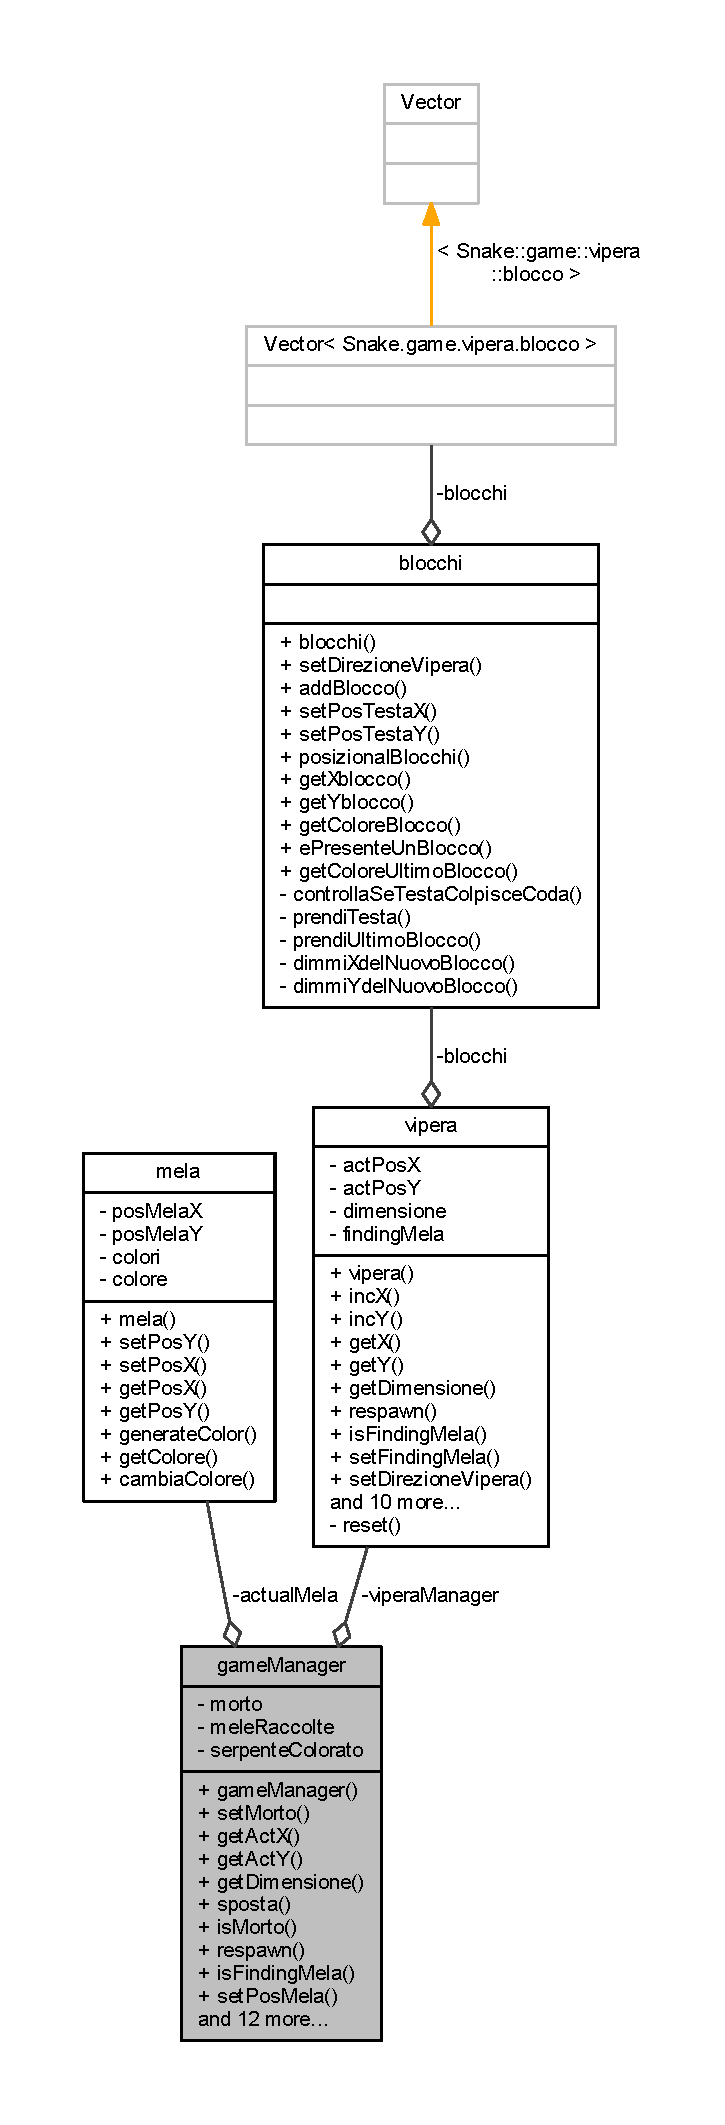
\includegraphics[height=550pt]{class_snake_1_1game_1_1utility_1_1game_manager__coll__graph}
\end{center}
\end{figure}
\subsection*{Public Member Functions}
\begin{DoxyCompactItemize}
\item 
\mbox{\hyperlink{class_snake_1_1game_1_1utility_1_1game_manager_a5751151adac49c0b87fa547f5e366dd9}{game\+Manager}} (boolean \mbox{\hyperlink{class_snake_1_1game_1_1utility_1_1game_manager_a23cfb877f1f20af97a29e6f61424aa80}{serpente\+Colorato}})
\begin{DoxyCompactList}\small\item\em Costruttore con parametri della classe. \end{DoxyCompactList}\item 
void \mbox{\hyperlink{class_snake_1_1game_1_1utility_1_1game_manager_a05b55f5dcc088b5655c5ff77c01f37ea}{set\+Morto}} (boolean v)
\begin{DoxyCompactList}\small\item\em Metodo che imposta l\textquotesingle{}attributo morto a seconda del parametro passato. \end{DoxyCompactList}\item 
int \mbox{\hyperlink{class_snake_1_1game_1_1utility_1_1game_manager_ae853a40673c27fff3315c5213c749814}{get\+ActX}} ()
\begin{DoxyCompactList}\small\item\em Ritorna la posizione X della vipera. \end{DoxyCompactList}\item 
int \mbox{\hyperlink{class_snake_1_1game_1_1utility_1_1game_manager_ae336e912feaec4a5e82fca472bde7f8f}{get\+ActY}} ()
\begin{DoxyCompactList}\small\item\em Ritorna la posizione X della vipera. \end{DoxyCompactList}\item 
int \mbox{\hyperlink{class_snake_1_1game_1_1utility_1_1game_manager_acda812adf1e0abdaf30cf3a2e2efaa07}{get\+Dimensione}} ()
\begin{DoxyCompactList}\small\item\em Ritorna la dimensione della vipera. \end{DoxyCompactList}\item 
void \mbox{\hyperlink{class_snake_1_1game_1_1utility_1_1game_manager_a9837912437f9fefee6140800ce8d6d76}{sposta}} (\mbox{\hyperlink{enum_snake_1_1game_1_1utility_1_1_directions}{Directions}} direzione)
\begin{DoxyCompactList}\small\item\em Sposta la vipera a seconda della direzione passata come parametro. \end{DoxyCompactList}\item 
boolean \mbox{\hyperlink{class_snake_1_1game_1_1utility_1_1game_manager_aa90b60b508f662fce93e3e8250b2c304}{is\+Morto}} ()
\begin{DoxyCompactList}\small\item\em Ritorna l\textquotesingle{}attributo morto della classe. \end{DoxyCompactList}\item 
void \mbox{\hyperlink{class_snake_1_1game_1_1utility_1_1game_manager_ac578ca44493fe34e6cb1b2093cf79341}{respawn}} ()
\begin{DoxyCompactList}\small\item\em Permette di restartare il gioco. \end{DoxyCompactList}\item 
boolean \mbox{\hyperlink{class_snake_1_1game_1_1utility_1_1game_manager_ad36cea66da3e5e8f3a9fdd8decd6f70b}{is\+Finding\+Mela}} ()
\begin{DoxyCompactList}\small\item\em Dice se la vipera sta cercando la mela. \end{DoxyCompactList}\item 
void \mbox{\hyperlink{class_snake_1_1game_1_1utility_1_1game_manager_a38aa4a80eb7f9db1e033f67dc1c220b0}{set\+Pos\+Mela}} (int pos\+MelaX, int pos\+MelaY)
\begin{DoxyCompactList}\small\item\em Imposta la posizione della mela a seconda dei parametri passati. \end{DoxyCompactList}\item 
void \mbox{\hyperlink{class_snake_1_1game_1_1utility_1_1game_manager_a3f6240b54a13e397255c9b3f7354cf45}{mela\+Presa}} ()
\begin{DoxyCompactList}\small\item\em Quando richiamato dice che la mela e\textquotesingle{} stata catturata quindi viene aggiunto un blocco alla vipera. \end{DoxyCompactList}\item 
int \mbox{\hyperlink{class_snake_1_1game_1_1utility_1_1game_manager_a5af927824d6cd9c9c30b0607cbdab546}{get\+Num\+Mele\+Prese}} ()
\begin{DoxyCompactList}\small\item\em Ritorna il numero di mele raccolte dalla vipera. \end{DoxyCompactList}\item 
void \mbox{\hyperlink{class_snake_1_1game_1_1utility_1_1game_manager_a6007259ace9d33bd56b9a6193e86df39}{set\+Direzione\+Vipera}} (\mbox{\hyperlink{enum_snake_1_1game_1_1utility_1_1_directions}{Directions}} dir)
\begin{DoxyCompactList}\small\item\em Imposta la direzione della vipera in base al parametro passato. \end{DoxyCompactList}\item 
int \mbox{\hyperlink{class_snake_1_1game_1_1utility_1_1game_manager_aae6590f1c2572c796a9ea154e3b16b27}{get\+Pos\+MelaX}} ()
\begin{DoxyCompactList}\small\item\em Ritorna la posizione X della mela. \end{DoxyCompactList}\item 
int \mbox{\hyperlink{class_snake_1_1game_1_1utility_1_1game_manager_ac23b89dc8711992dc3124c04888a1365}{get\+Pos\+MelaY}} ()
\begin{DoxyCompactList}\small\item\em Ritorna la posizione Y della mela. \end{DoxyCompactList}\item 
void \mbox{\hyperlink{class_snake_1_1game_1_1utility_1_1game_manager_a169584b55e994918baf671fe1c741e39}{set\+Finding\+Mela}} (boolean b)
\begin{DoxyCompactList}\small\item\em Permette di dire al serpente se deve trovare oppure no la mela. \end{DoxyCompactList}\item 
int \mbox{\hyperlink{class_snake_1_1game_1_1utility_1_1game_manager_a88318c562485640585510cbd35e76b07}{pos\+Xblocco}} (int i)
\begin{DoxyCompactList}\small\item\em Ritorna la posizione X del blocco identificato da parametro. \end{DoxyCompactList}\item 
int \mbox{\hyperlink{class_snake_1_1game_1_1utility_1_1game_manager_ac26b1474a291f2f7546e2e1cda1410b8}{pos\+Yblocco}} (int i)
\begin{DoxyCompactList}\small\item\em Ritorna la posizione Y del blocco identificato da parametro. \end{DoxyCompactList}\item 
Color \mbox{\hyperlink{class_snake_1_1game_1_1utility_1_1game_manager_a15fad4646c986312b476543b2f7e547a}{get\+Colore\+Mela}} ()
\begin{DoxyCompactList}\small\item\em Ritorna il colore della mela. \end{DoxyCompactList}\item 
boolean \mbox{\hyperlink{class_snake_1_1game_1_1utility_1_1game_manager_ac24833a417b3bd7c60e29ed5b7edc29f}{e\+Presente\+Un\+Blocco}} (int x, int y)
\begin{DoxyCompactList}\small\item\em Dice se e\textquotesingle{} presente un blocco nella posizione X e Y dello schermo. \end{DoxyCompactList}\item 
Color \mbox{\hyperlink{class_snake_1_1game_1_1utility_1_1game_manager_a1afbc9b85396f53e6180eab2e5a36d4d}{get\+Colore\+Ultimo\+Blocco}} ()
\begin{DoxyCompactList}\small\item\em Restituisce il colore dell\textquotesingle{}ultimo blocco in coda alla vipera. \end{DoxyCompactList}\item 
Boolean \mbox{\hyperlink{class_snake_1_1game_1_1utility_1_1game_manager_adf69d52c2b16c0b681a384f734f9dd0f}{get\+Serpente\+Colorato}} ()
\begin{DoxyCompactList}\small\item\em Dice se il serpente e\textquotesingle{} colorato oppure no. \end{DoxyCompactList}\end{DoxyCompactItemize}
\subsection*{Private Attributes}
\begin{DoxyCompactItemize}
\item 
\mbox{\hyperlink{class_snake_1_1game_1_1vipera_1_1vipera}{vipera}} \mbox{\hyperlink{class_snake_1_1game_1_1utility_1_1game_manager_ad03d565374455808665272d6365c9bca}{vipera\+Manager}}
\item 
boolean \mbox{\hyperlink{class_snake_1_1game_1_1utility_1_1game_manager_a415d6bb79054489c86349a855c1015be}{morto}}
\item 
\mbox{\hyperlink{class_snake_1_1game_1_1vipera_1_1mela}{mela}} \mbox{\hyperlink{class_snake_1_1game_1_1utility_1_1game_manager_a8ed97a1e91168bdb3e5d2dea4e59a977}{actual\+Mela}}
\item 
int \mbox{\hyperlink{class_snake_1_1game_1_1utility_1_1game_manager_a6ccf94c481d483cdef8cca4743754db4}{mele\+Raccolte}} =0
\item 
boolean \mbox{\hyperlink{class_snake_1_1game_1_1utility_1_1game_manager_a23cfb877f1f20af97a29e6f61424aa80}{serpente\+Colorato}}
\end{DoxyCompactItemize}


\subsection{Detailed Description}
\begin{DoxyAuthor}{Author}
Saccani Federico, \href{mailto:federico.saccani01@gmail.com}{\tt federico.\+saccani01@gmail.\+com} 
\end{DoxyAuthor}
\begin{DoxyVersion}{Version}
1.\+0 ~\newline
La classe viene utilizzata per gestire tutto il serpente e le relative mele 
\end{DoxyVersion}


Definition at line 15 of file game\+Manager.\+java.



\subsection{Constructor \& Destructor Documentation}
\mbox{\Hypertarget{class_snake_1_1game_1_1utility_1_1game_manager_a5751151adac49c0b87fa547f5e366dd9}\label{class_snake_1_1game_1_1utility_1_1game_manager_a5751151adac49c0b87fa547f5e366dd9}} 
\index{Snake\+::game\+::utility\+::game\+Manager@{Snake\+::game\+::utility\+::game\+Manager}!game\+Manager@{game\+Manager}}
\index{game\+Manager@{game\+Manager}!Snake\+::game\+::utility\+::game\+Manager@{Snake\+::game\+::utility\+::game\+Manager}}
\subsubsection{\texorpdfstring{game\+Manager()}{gameManager()}}
{\footnotesize\ttfamily \mbox{\hyperlink{class_snake_1_1game_1_1utility_1_1game_manager}{game\+Manager}} (\begin{DoxyParamCaption}\item[{boolean}]{serpente\+Colorato }\end{DoxyParamCaption})}



Costruttore con parametri della classe. 


\begin{DoxyParams}{Parameters}
{\em serpente\+Colorato} & se il serpente deve colorarsi in base all\textquotesingle{}ultima mela presa \\
\hline
\end{DoxyParams}


Definition at line 34 of file game\+Manager.\+java.



\subsection{Member Function Documentation}
\mbox{\Hypertarget{class_snake_1_1game_1_1utility_1_1game_manager_ac24833a417b3bd7c60e29ed5b7edc29f}\label{class_snake_1_1game_1_1utility_1_1game_manager_ac24833a417b3bd7c60e29ed5b7edc29f}} 
\index{Snake\+::game\+::utility\+::game\+Manager@{Snake\+::game\+::utility\+::game\+Manager}!e\+Presente\+Un\+Blocco@{e\+Presente\+Un\+Blocco}}
\index{e\+Presente\+Un\+Blocco@{e\+Presente\+Un\+Blocco}!Snake\+::game\+::utility\+::game\+Manager@{Snake\+::game\+::utility\+::game\+Manager}}
\subsubsection{\texorpdfstring{e\+Presente\+Un\+Blocco()}{ePresenteUnBlocco()}}
{\footnotesize\ttfamily boolean e\+Presente\+Un\+Blocco (\begin{DoxyParamCaption}\item[{int}]{x,  }\item[{int}]{y }\end{DoxyParamCaption})}



Dice se e\textquotesingle{} presente un blocco nella posizione X e Y dello schermo. 


\begin{DoxyParams}{Parameters}
{\em x} & posizione X dello schermo \\
\hline
{\em y} & posizione Y dello schermo \\
\hline
\end{DoxyParams}


Definition at line 212 of file game\+Manager.\+java.

Here is the call graph for this function\+:
\nopagebreak
\begin{figure}[H]
\begin{center}
\leavevmode
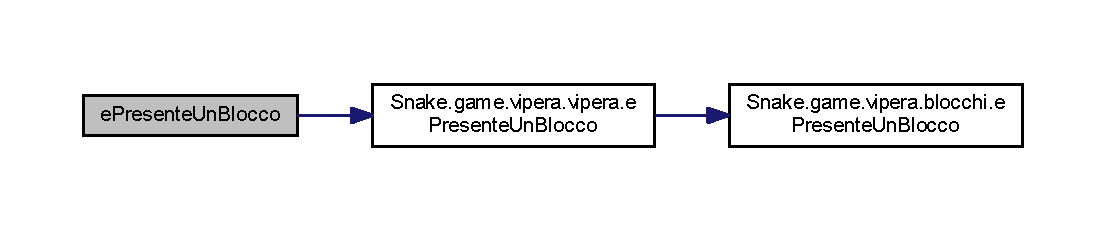
\includegraphics[width=350pt]{class_snake_1_1game_1_1utility_1_1game_manager_ac24833a417b3bd7c60e29ed5b7edc29f_cgraph}
\end{center}
\end{figure}
Here is the caller graph for this function\+:
\nopagebreak
\begin{figure}[H]
\begin{center}
\leavevmode
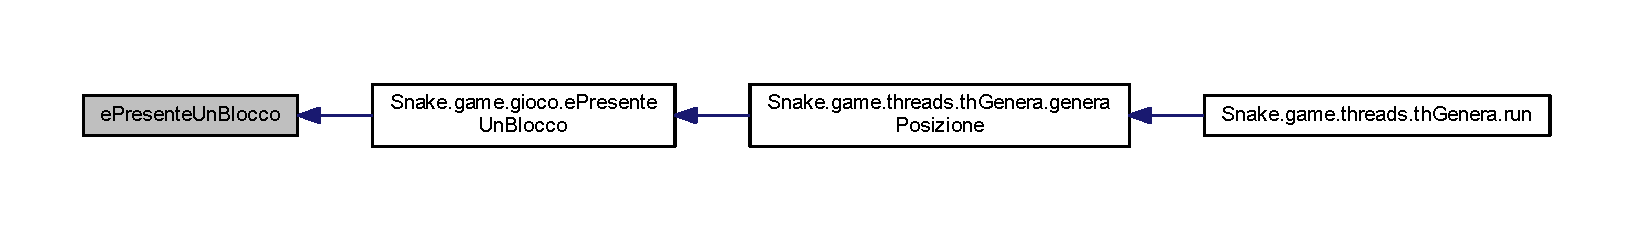
\includegraphics[width=350pt]{class_snake_1_1game_1_1utility_1_1game_manager_ac24833a417b3bd7c60e29ed5b7edc29f_icgraph}
\end{center}
\end{figure}
\mbox{\Hypertarget{class_snake_1_1game_1_1utility_1_1game_manager_ae853a40673c27fff3315c5213c749814}\label{class_snake_1_1game_1_1utility_1_1game_manager_ae853a40673c27fff3315c5213c749814}} 
\index{Snake\+::game\+::utility\+::game\+Manager@{Snake\+::game\+::utility\+::game\+Manager}!get\+ActX@{get\+ActX}}
\index{get\+ActX@{get\+ActX}!Snake\+::game\+::utility\+::game\+Manager@{Snake\+::game\+::utility\+::game\+Manager}}
\subsubsection{\texorpdfstring{get\+Act\+X()}{getActX()}}
{\footnotesize\ttfamily int get\+ActX (\begin{DoxyParamCaption}{ }\end{DoxyParamCaption})}



Ritorna la posizione X della vipera. 



Definition at line 52 of file game\+Manager.\+java.

Here is the call graph for this function\+:
\nopagebreak
\begin{figure}[H]
\begin{center}
\leavevmode
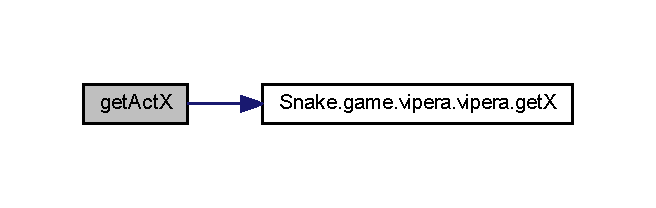
\includegraphics[width=315pt]{class_snake_1_1game_1_1utility_1_1game_manager_ae853a40673c27fff3315c5213c749814_cgraph}
\end{center}
\end{figure}
Here is the caller graph for this function\+:
\nopagebreak
\begin{figure}[H]
\begin{center}
\leavevmode
\includegraphics[width=350pt]{class_snake_1_1game_1_1utility_1_1game_manager_ae853a40673c27fff3315c5213c749814_icgraph}
\end{center}
\end{figure}
\mbox{\Hypertarget{class_snake_1_1game_1_1utility_1_1game_manager_ae336e912feaec4a5e82fca472bde7f8f}\label{class_snake_1_1game_1_1utility_1_1game_manager_ae336e912feaec4a5e82fca472bde7f8f}} 
\index{Snake\+::game\+::utility\+::game\+Manager@{Snake\+::game\+::utility\+::game\+Manager}!get\+ActY@{get\+ActY}}
\index{get\+ActY@{get\+ActY}!Snake\+::game\+::utility\+::game\+Manager@{Snake\+::game\+::utility\+::game\+Manager}}
\subsubsection{\texorpdfstring{get\+Act\+Y()}{getActY()}}
{\footnotesize\ttfamily int get\+ActY (\begin{DoxyParamCaption}{ }\end{DoxyParamCaption})}



Ritorna la posizione X della vipera. 



Definition at line 58 of file game\+Manager.\+java.

Here is the call graph for this function\+:
\nopagebreak
\begin{figure}[H]
\begin{center}
\leavevmode
\includegraphics[width=318pt]{class_snake_1_1game_1_1utility_1_1game_manager_ae336e912feaec4a5e82fca472bde7f8f_cgraph}
\end{center}
\end{figure}
Here is the caller graph for this function\+:
\nopagebreak
\begin{figure}[H]
\begin{center}
\leavevmode
\includegraphics[width=350pt]{class_snake_1_1game_1_1utility_1_1game_manager_ae336e912feaec4a5e82fca472bde7f8f_icgraph}
\end{center}
\end{figure}
\mbox{\Hypertarget{class_snake_1_1game_1_1utility_1_1game_manager_a15fad4646c986312b476543b2f7e547a}\label{class_snake_1_1game_1_1utility_1_1game_manager_a15fad4646c986312b476543b2f7e547a}} 
\index{Snake\+::game\+::utility\+::game\+Manager@{Snake\+::game\+::utility\+::game\+Manager}!get\+Colore\+Mela@{get\+Colore\+Mela}}
\index{get\+Colore\+Mela@{get\+Colore\+Mela}!Snake\+::game\+::utility\+::game\+Manager@{Snake\+::game\+::utility\+::game\+Manager}}
\subsubsection{\texorpdfstring{get\+Colore\+Mela()}{getColoreMela()}}
{\footnotesize\ttfamily Color get\+Colore\+Mela (\begin{DoxyParamCaption}{ }\end{DoxyParamCaption})}



Ritorna il colore della mela. 



Definition at line 202 of file game\+Manager.\+java.

Here is the call graph for this function\+:
\nopagebreak
\begin{figure}[H]
\begin{center}
\leavevmode
\includegraphics[width=335pt]{class_snake_1_1game_1_1utility_1_1game_manager_a15fad4646c986312b476543b2f7e547a_cgraph}
\end{center}
\end{figure}
Here is the caller graph for this function\+:
\nopagebreak
\begin{figure}[H]
\begin{center}
\leavevmode
\includegraphics[width=350pt]{class_snake_1_1game_1_1utility_1_1game_manager_a15fad4646c986312b476543b2f7e547a_icgraph}
\end{center}
\end{figure}
\mbox{\Hypertarget{class_snake_1_1game_1_1utility_1_1game_manager_a1afbc9b85396f53e6180eab2e5a36d4d}\label{class_snake_1_1game_1_1utility_1_1game_manager_a1afbc9b85396f53e6180eab2e5a36d4d}} 
\index{Snake\+::game\+::utility\+::game\+Manager@{Snake\+::game\+::utility\+::game\+Manager}!get\+Colore\+Ultimo\+Blocco@{get\+Colore\+Ultimo\+Blocco}}
\index{get\+Colore\+Ultimo\+Blocco@{get\+Colore\+Ultimo\+Blocco}!Snake\+::game\+::utility\+::game\+Manager@{Snake\+::game\+::utility\+::game\+Manager}}
\subsubsection{\texorpdfstring{get\+Colore\+Ultimo\+Blocco()}{getColoreUltimoBlocco()}}
{\footnotesize\ttfamily Color get\+Colore\+Ultimo\+Blocco (\begin{DoxyParamCaption}{ }\end{DoxyParamCaption})}



Restituisce il colore dell\textquotesingle{}ultimo blocco in coda alla vipera. 



Definition at line 219 of file game\+Manager.\+java.

Here is the call graph for this function\+:
\nopagebreak
\begin{figure}[H]
\begin{center}
\leavevmode
\includegraphics[width=350pt]{class_snake_1_1game_1_1utility_1_1game_manager_a1afbc9b85396f53e6180eab2e5a36d4d_cgraph}
\end{center}
\end{figure}
Here is the caller graph for this function\+:
\nopagebreak
\begin{figure}[H]
\begin{center}
\leavevmode
\includegraphics[width=350pt]{class_snake_1_1game_1_1utility_1_1game_manager_a1afbc9b85396f53e6180eab2e5a36d4d_icgraph}
\end{center}
\end{figure}
\mbox{\Hypertarget{class_snake_1_1game_1_1utility_1_1game_manager_acda812adf1e0abdaf30cf3a2e2efaa07}\label{class_snake_1_1game_1_1utility_1_1game_manager_acda812adf1e0abdaf30cf3a2e2efaa07}} 
\index{Snake\+::game\+::utility\+::game\+Manager@{Snake\+::game\+::utility\+::game\+Manager}!get\+Dimensione@{get\+Dimensione}}
\index{get\+Dimensione@{get\+Dimensione}!Snake\+::game\+::utility\+::game\+Manager@{Snake\+::game\+::utility\+::game\+Manager}}
\subsubsection{\texorpdfstring{get\+Dimensione()}{getDimensione()}}
{\footnotesize\ttfamily int get\+Dimensione (\begin{DoxyParamCaption}{ }\end{DoxyParamCaption})}



Ritorna la dimensione della vipera. 



Definition at line 64 of file game\+Manager.\+java.

Here is the call graph for this function\+:
\nopagebreak
\begin{figure}[H]
\begin{center}
\leavevmode
\includegraphics[width=340pt]{class_snake_1_1game_1_1utility_1_1game_manager_acda812adf1e0abdaf30cf3a2e2efaa07_cgraph}
\end{center}
\end{figure}
Here is the caller graph for this function\+:
\nopagebreak
\begin{figure}[H]
\begin{center}
\leavevmode
\includegraphics[width=350pt]{class_snake_1_1game_1_1utility_1_1game_manager_acda812adf1e0abdaf30cf3a2e2efaa07_icgraph}
\end{center}
\end{figure}
\mbox{\Hypertarget{class_snake_1_1game_1_1utility_1_1game_manager_a5af927824d6cd9c9c30b0607cbdab546}\label{class_snake_1_1game_1_1utility_1_1game_manager_a5af927824d6cd9c9c30b0607cbdab546}} 
\index{Snake\+::game\+::utility\+::game\+Manager@{Snake\+::game\+::utility\+::game\+Manager}!get\+Num\+Mele\+Prese@{get\+Num\+Mele\+Prese}}
\index{get\+Num\+Mele\+Prese@{get\+Num\+Mele\+Prese}!Snake\+::game\+::utility\+::game\+Manager@{Snake\+::game\+::utility\+::game\+Manager}}
\subsubsection{\texorpdfstring{get\+Num\+Mele\+Prese()}{getNumMelePrese()}}
{\footnotesize\ttfamily int get\+Num\+Mele\+Prese (\begin{DoxyParamCaption}{ }\end{DoxyParamCaption})}



Ritorna il numero di mele raccolte dalla vipera. 



Definition at line 147 of file game\+Manager.\+java.

Here is the caller graph for this function\+:
\nopagebreak
\begin{figure}[H]
\begin{center}
\leavevmode
\includegraphics[width=350pt]{class_snake_1_1game_1_1utility_1_1game_manager_a5af927824d6cd9c9c30b0607cbdab546_icgraph}
\end{center}
\end{figure}
\mbox{\Hypertarget{class_snake_1_1game_1_1utility_1_1game_manager_aae6590f1c2572c796a9ea154e3b16b27}\label{class_snake_1_1game_1_1utility_1_1game_manager_aae6590f1c2572c796a9ea154e3b16b27}} 
\index{Snake\+::game\+::utility\+::game\+Manager@{Snake\+::game\+::utility\+::game\+Manager}!get\+Pos\+MelaX@{get\+Pos\+MelaX}}
\index{get\+Pos\+MelaX@{get\+Pos\+MelaX}!Snake\+::game\+::utility\+::game\+Manager@{Snake\+::game\+::utility\+::game\+Manager}}
\subsubsection{\texorpdfstring{get\+Pos\+Mela\+X()}{getPosMelaX()}}
{\footnotesize\ttfamily int get\+Pos\+MelaX (\begin{DoxyParamCaption}{ }\end{DoxyParamCaption})}



Ritorna la posizione X della mela. 



Definition at line 163 of file game\+Manager.\+java.

Here is the call graph for this function\+:
\nopagebreak
\begin{figure}[H]
\begin{center}
\leavevmode
\includegraphics[width=350pt]{class_snake_1_1game_1_1utility_1_1game_manager_aae6590f1c2572c796a9ea154e3b16b27_cgraph}
\end{center}
\end{figure}
Here is the caller graph for this function\+:
\nopagebreak
\begin{figure}[H]
\begin{center}
\leavevmode
\includegraphics[width=350pt]{class_snake_1_1game_1_1utility_1_1game_manager_aae6590f1c2572c796a9ea154e3b16b27_icgraph}
\end{center}
\end{figure}
\mbox{\Hypertarget{class_snake_1_1game_1_1utility_1_1game_manager_ac23b89dc8711992dc3124c04888a1365}\label{class_snake_1_1game_1_1utility_1_1game_manager_ac23b89dc8711992dc3124c04888a1365}} 
\index{Snake\+::game\+::utility\+::game\+Manager@{Snake\+::game\+::utility\+::game\+Manager}!get\+Pos\+MelaY@{get\+Pos\+MelaY}}
\index{get\+Pos\+MelaY@{get\+Pos\+MelaY}!Snake\+::game\+::utility\+::game\+Manager@{Snake\+::game\+::utility\+::game\+Manager}}
\subsubsection{\texorpdfstring{get\+Pos\+Mela\+Y()}{getPosMelaY()}}
{\footnotesize\ttfamily int get\+Pos\+MelaY (\begin{DoxyParamCaption}{ }\end{DoxyParamCaption})}



Ritorna la posizione Y della mela. 



Definition at line 169 of file game\+Manager.\+java.

Here is the call graph for this function\+:
\nopagebreak
\begin{figure}[H]
\begin{center}
\leavevmode
\includegraphics[width=350pt]{class_snake_1_1game_1_1utility_1_1game_manager_ac23b89dc8711992dc3124c04888a1365_cgraph}
\end{center}
\end{figure}
Here is the caller graph for this function\+:
\nopagebreak
\begin{figure}[H]
\begin{center}
\leavevmode
\includegraphics[width=350pt]{class_snake_1_1game_1_1utility_1_1game_manager_ac23b89dc8711992dc3124c04888a1365_icgraph}
\end{center}
\end{figure}
\mbox{\Hypertarget{class_snake_1_1game_1_1utility_1_1game_manager_adf69d52c2b16c0b681a384f734f9dd0f}\label{class_snake_1_1game_1_1utility_1_1game_manager_adf69d52c2b16c0b681a384f734f9dd0f}} 
\index{Snake\+::game\+::utility\+::game\+Manager@{Snake\+::game\+::utility\+::game\+Manager}!get\+Serpente\+Colorato@{get\+Serpente\+Colorato}}
\index{get\+Serpente\+Colorato@{get\+Serpente\+Colorato}!Snake\+::game\+::utility\+::game\+Manager@{Snake\+::game\+::utility\+::game\+Manager}}
\subsubsection{\texorpdfstring{get\+Serpente\+Colorato()}{getSerpenteColorato()}}
{\footnotesize\ttfamily Boolean get\+Serpente\+Colorato (\begin{DoxyParamCaption}{ }\end{DoxyParamCaption})}



Dice se il serpente e\textquotesingle{} colorato oppure no. 



Definition at line 225 of file game\+Manager.\+java.

Here is the caller graph for this function\+:
\nopagebreak
\begin{figure}[H]
\begin{center}
\leavevmode
\includegraphics[width=350pt]{class_snake_1_1game_1_1utility_1_1game_manager_adf69d52c2b16c0b681a384f734f9dd0f_icgraph}
\end{center}
\end{figure}
\mbox{\Hypertarget{class_snake_1_1game_1_1utility_1_1game_manager_ad36cea66da3e5e8f3a9fdd8decd6f70b}\label{class_snake_1_1game_1_1utility_1_1game_manager_ad36cea66da3e5e8f3a9fdd8decd6f70b}} 
\index{Snake\+::game\+::utility\+::game\+Manager@{Snake\+::game\+::utility\+::game\+Manager}!is\+Finding\+Mela@{is\+Finding\+Mela}}
\index{is\+Finding\+Mela@{is\+Finding\+Mela}!Snake\+::game\+::utility\+::game\+Manager@{Snake\+::game\+::utility\+::game\+Manager}}
\subsubsection{\texorpdfstring{is\+Finding\+Mela()}{isFindingMela()}}
{\footnotesize\ttfamily boolean is\+Finding\+Mela (\begin{DoxyParamCaption}{ }\end{DoxyParamCaption})}



Dice se la vipera sta cercando la mela. 



Definition at line 116 of file game\+Manager.\+java.

Here is the call graph for this function\+:
\nopagebreak
\begin{figure}[H]
\begin{center}
\leavevmode
\includegraphics[width=330pt]{class_snake_1_1game_1_1utility_1_1game_manager_ad36cea66da3e5e8f3a9fdd8decd6f70b_cgraph}
\end{center}
\end{figure}
Here is the caller graph for this function\+:
\nopagebreak
\begin{figure}[H]
\begin{center}
\leavevmode
\includegraphics[width=350pt]{class_snake_1_1game_1_1utility_1_1game_manager_ad36cea66da3e5e8f3a9fdd8decd6f70b_icgraph}
\end{center}
\end{figure}
\mbox{\Hypertarget{class_snake_1_1game_1_1utility_1_1game_manager_aa90b60b508f662fce93e3e8250b2c304}\label{class_snake_1_1game_1_1utility_1_1game_manager_aa90b60b508f662fce93e3e8250b2c304}} 
\index{Snake\+::game\+::utility\+::game\+Manager@{Snake\+::game\+::utility\+::game\+Manager}!is\+Morto@{is\+Morto}}
\index{is\+Morto@{is\+Morto}!Snake\+::game\+::utility\+::game\+Manager@{Snake\+::game\+::utility\+::game\+Manager}}
\subsubsection{\texorpdfstring{is\+Morto()}{isMorto()}}
{\footnotesize\ttfamily boolean is\+Morto (\begin{DoxyParamCaption}{ }\end{DoxyParamCaption})}



Ritorna l\textquotesingle{}attributo morto della classe. 



Definition at line 99 of file game\+Manager.\+java.

Here is the caller graph for this function\+:
\nopagebreak
\begin{figure}[H]
\begin{center}
\leavevmode
\includegraphics[width=350pt]{class_snake_1_1game_1_1utility_1_1game_manager_aa90b60b508f662fce93e3e8250b2c304_icgraph}
\end{center}
\end{figure}
\mbox{\Hypertarget{class_snake_1_1game_1_1utility_1_1game_manager_a3f6240b54a13e397255c9b3f7354cf45}\label{class_snake_1_1game_1_1utility_1_1game_manager_a3f6240b54a13e397255c9b3f7354cf45}} 
\index{Snake\+::game\+::utility\+::game\+Manager@{Snake\+::game\+::utility\+::game\+Manager}!mela\+Presa@{mela\+Presa}}
\index{mela\+Presa@{mela\+Presa}!Snake\+::game\+::utility\+::game\+Manager@{Snake\+::game\+::utility\+::game\+Manager}}
\subsubsection{\texorpdfstring{mela\+Presa()}{melaPresa()}}
{\footnotesize\ttfamily void mela\+Presa (\begin{DoxyParamCaption}{ }\end{DoxyParamCaption})}



Quando richiamato dice che la mela e\textquotesingle{} stata catturata quindi viene aggiunto un blocco alla vipera. 



Definition at line 134 of file game\+Manager.\+java.

Here is the call graph for this function\+:
\nopagebreak
\begin{figure}[H]
\begin{center}
\leavevmode
\includegraphics[width=350pt]{class_snake_1_1game_1_1utility_1_1game_manager_a3f6240b54a13e397255c9b3f7354cf45_cgraph}
\end{center}
\end{figure}
Here is the caller graph for this function\+:
\nopagebreak
\begin{figure}[H]
\begin{center}
\leavevmode
\includegraphics[width=350pt]{class_snake_1_1game_1_1utility_1_1game_manager_a3f6240b54a13e397255c9b3f7354cf45_icgraph}
\end{center}
\end{figure}
\mbox{\Hypertarget{class_snake_1_1game_1_1utility_1_1game_manager_a88318c562485640585510cbd35e76b07}\label{class_snake_1_1game_1_1utility_1_1game_manager_a88318c562485640585510cbd35e76b07}} 
\index{Snake\+::game\+::utility\+::game\+Manager@{Snake\+::game\+::utility\+::game\+Manager}!pos\+Xblocco@{pos\+Xblocco}}
\index{pos\+Xblocco@{pos\+Xblocco}!Snake\+::game\+::utility\+::game\+Manager@{Snake\+::game\+::utility\+::game\+Manager}}
\subsubsection{\texorpdfstring{pos\+Xblocco()}{posXblocco()}}
{\footnotesize\ttfamily int pos\+Xblocco (\begin{DoxyParamCaption}\item[{int}]{i }\end{DoxyParamCaption})}



Ritorna la posizione X del blocco identificato da parametro. 


\begin{DoxyParams}{Parameters}
{\em i} & identificativo del blocco \\
\hline
\end{DoxyParams}


Definition at line 187 of file game\+Manager.\+java.

Here is the call graph for this function\+:
\nopagebreak
\begin{figure}[H]
\begin{center}
\leavevmode
\includegraphics[width=350pt]{class_snake_1_1game_1_1utility_1_1game_manager_a88318c562485640585510cbd35e76b07_cgraph}
\end{center}
\end{figure}
Here is the caller graph for this function\+:
\nopagebreak
\begin{figure}[H]
\begin{center}
\leavevmode
\includegraphics[width=350pt]{class_snake_1_1game_1_1utility_1_1game_manager_a88318c562485640585510cbd35e76b07_icgraph}
\end{center}
\end{figure}
\mbox{\Hypertarget{class_snake_1_1game_1_1utility_1_1game_manager_ac26b1474a291f2f7546e2e1cda1410b8}\label{class_snake_1_1game_1_1utility_1_1game_manager_ac26b1474a291f2f7546e2e1cda1410b8}} 
\index{Snake\+::game\+::utility\+::game\+Manager@{Snake\+::game\+::utility\+::game\+Manager}!pos\+Yblocco@{pos\+Yblocco}}
\index{pos\+Yblocco@{pos\+Yblocco}!Snake\+::game\+::utility\+::game\+Manager@{Snake\+::game\+::utility\+::game\+Manager}}
\subsubsection{\texorpdfstring{pos\+Yblocco()}{posYblocco()}}
{\footnotesize\ttfamily int pos\+Yblocco (\begin{DoxyParamCaption}\item[{int}]{i }\end{DoxyParamCaption})}



Ritorna la posizione Y del blocco identificato da parametro. 


\begin{DoxyParams}{Parameters}
{\em i} & identificativo del blocco \\
\hline
\end{DoxyParams}


Definition at line 195 of file game\+Manager.\+java.

Here is the call graph for this function\+:
\nopagebreak
\begin{figure}[H]
\begin{center}
\leavevmode
\includegraphics[width=350pt]{class_snake_1_1game_1_1utility_1_1game_manager_ac26b1474a291f2f7546e2e1cda1410b8_cgraph}
\end{center}
\end{figure}
Here is the caller graph for this function\+:
\nopagebreak
\begin{figure}[H]
\begin{center}
\leavevmode
\includegraphics[width=350pt]{class_snake_1_1game_1_1utility_1_1game_manager_ac26b1474a291f2f7546e2e1cda1410b8_icgraph}
\end{center}
\end{figure}
\mbox{\Hypertarget{class_snake_1_1game_1_1utility_1_1game_manager_ac578ca44493fe34e6cb1b2093cf79341}\label{class_snake_1_1game_1_1utility_1_1game_manager_ac578ca44493fe34e6cb1b2093cf79341}} 
\index{Snake\+::game\+::utility\+::game\+Manager@{Snake\+::game\+::utility\+::game\+Manager}!respawn@{respawn}}
\index{respawn@{respawn}!Snake\+::game\+::utility\+::game\+Manager@{Snake\+::game\+::utility\+::game\+Manager}}
\subsubsection{\texorpdfstring{respawn()}{respawn()}}
{\footnotesize\ttfamily void respawn (\begin{DoxyParamCaption}{ }\end{DoxyParamCaption})}



Permette di restartare il gioco. 



Definition at line 106 of file game\+Manager.\+java.

Here is the call graph for this function\+:
\nopagebreak
\begin{figure}[H]
\begin{center}
\leavevmode
\includegraphics[width=350pt]{class_snake_1_1game_1_1utility_1_1game_manager_ac578ca44493fe34e6cb1b2093cf79341_cgraph}
\end{center}
\end{figure}
Here is the caller graph for this function\+:
\nopagebreak
\begin{figure}[H]
\begin{center}
\leavevmode
\includegraphics[width=350pt]{class_snake_1_1game_1_1utility_1_1game_manager_ac578ca44493fe34e6cb1b2093cf79341_icgraph}
\end{center}
\end{figure}
\mbox{\Hypertarget{class_snake_1_1game_1_1utility_1_1game_manager_a6007259ace9d33bd56b9a6193e86df39}\label{class_snake_1_1game_1_1utility_1_1game_manager_a6007259ace9d33bd56b9a6193e86df39}} 
\index{Snake\+::game\+::utility\+::game\+Manager@{Snake\+::game\+::utility\+::game\+Manager}!set\+Direzione\+Vipera@{set\+Direzione\+Vipera}}
\index{set\+Direzione\+Vipera@{set\+Direzione\+Vipera}!Snake\+::game\+::utility\+::game\+Manager@{Snake\+::game\+::utility\+::game\+Manager}}
\subsubsection{\texorpdfstring{set\+Direzione\+Vipera()}{setDirezioneVipera()}}
{\footnotesize\ttfamily void set\+Direzione\+Vipera (\begin{DoxyParamCaption}\item[{\mbox{\hyperlink{enum_snake_1_1game_1_1utility_1_1_directions}{Directions}}}]{dir }\end{DoxyParamCaption})}



Imposta la direzione della vipera in base al parametro passato. 


\begin{DoxyParams}{Parameters}
{\em dir} & direzione vipera \\
\hline
\end{DoxyParams}


Definition at line 156 of file game\+Manager.\+java.

Here is the call graph for this function\+:
\nopagebreak
\begin{figure}[H]
\begin{center}
\leavevmode
\includegraphics[width=350pt]{class_snake_1_1game_1_1utility_1_1game_manager_a6007259ace9d33bd56b9a6193e86df39_cgraph}
\end{center}
\end{figure}
Here is the caller graph for this function\+:
\nopagebreak
\begin{figure}[H]
\begin{center}
\leavevmode
\includegraphics[width=350pt]{class_snake_1_1game_1_1utility_1_1game_manager_a6007259ace9d33bd56b9a6193e86df39_icgraph}
\end{center}
\end{figure}
\mbox{\Hypertarget{class_snake_1_1game_1_1utility_1_1game_manager_a169584b55e994918baf671fe1c741e39}\label{class_snake_1_1game_1_1utility_1_1game_manager_a169584b55e994918baf671fe1c741e39}} 
\index{Snake\+::game\+::utility\+::game\+Manager@{Snake\+::game\+::utility\+::game\+Manager}!set\+Finding\+Mela@{set\+Finding\+Mela}}
\index{set\+Finding\+Mela@{set\+Finding\+Mela}!Snake\+::game\+::utility\+::game\+Manager@{Snake\+::game\+::utility\+::game\+Manager}}
\subsubsection{\texorpdfstring{set\+Finding\+Mela()}{setFindingMela()}}
{\footnotesize\ttfamily void set\+Finding\+Mela (\begin{DoxyParamCaption}\item[{boolean}]{b }\end{DoxyParamCaption})}



Permette di dire al serpente se deve trovare oppure no la mela. 


\begin{DoxyParams}{Parameters}
{\em b} & booleana \\
\hline
\end{DoxyParams}


Definition at line 178 of file game\+Manager.\+java.

Here is the call graph for this function\+:
\nopagebreak
\begin{figure}[H]
\begin{center}
\leavevmode
\includegraphics[width=342pt]{class_snake_1_1game_1_1utility_1_1game_manager_a169584b55e994918baf671fe1c741e39_cgraph}
\end{center}
\end{figure}
Here is the caller graph for this function\+:
\nopagebreak
\begin{figure}[H]
\begin{center}
\leavevmode
\includegraphics[width=350pt]{class_snake_1_1game_1_1utility_1_1game_manager_a169584b55e994918baf671fe1c741e39_icgraph}
\end{center}
\end{figure}
\mbox{\Hypertarget{class_snake_1_1game_1_1utility_1_1game_manager_a05b55f5dcc088b5655c5ff77c01f37ea}\label{class_snake_1_1game_1_1utility_1_1game_manager_a05b55f5dcc088b5655c5ff77c01f37ea}} 
\index{Snake\+::game\+::utility\+::game\+Manager@{Snake\+::game\+::utility\+::game\+Manager}!set\+Morto@{set\+Morto}}
\index{set\+Morto@{set\+Morto}!Snake\+::game\+::utility\+::game\+Manager@{Snake\+::game\+::utility\+::game\+Manager}}
\subsubsection{\texorpdfstring{set\+Morto()}{setMorto()}}
{\footnotesize\ttfamily void set\+Morto (\begin{DoxyParamCaption}\item[{boolean}]{v }\end{DoxyParamCaption})}



Metodo che imposta l\textquotesingle{}attributo morto a seconda del parametro passato. 


\begin{DoxyParams}{Parameters}
{\em v} & stato \\
\hline
\end{DoxyParams}


Definition at line 46 of file game\+Manager.\+java.

Here is the caller graph for this function\+:
\nopagebreak
\begin{figure}[H]
\begin{center}
\leavevmode
\includegraphics[width=350pt]{class_snake_1_1game_1_1utility_1_1game_manager_a05b55f5dcc088b5655c5ff77c01f37ea_icgraph}
\end{center}
\end{figure}
\mbox{\Hypertarget{class_snake_1_1game_1_1utility_1_1game_manager_a38aa4a80eb7f9db1e033f67dc1c220b0}\label{class_snake_1_1game_1_1utility_1_1game_manager_a38aa4a80eb7f9db1e033f67dc1c220b0}} 
\index{Snake\+::game\+::utility\+::game\+Manager@{Snake\+::game\+::utility\+::game\+Manager}!set\+Pos\+Mela@{set\+Pos\+Mela}}
\index{set\+Pos\+Mela@{set\+Pos\+Mela}!Snake\+::game\+::utility\+::game\+Manager@{Snake\+::game\+::utility\+::game\+Manager}}
\subsubsection{\texorpdfstring{set\+Pos\+Mela()}{setPosMela()}}
{\footnotesize\ttfamily void set\+Pos\+Mela (\begin{DoxyParamCaption}\item[{int}]{pos\+MelaX,  }\item[{int}]{pos\+MelaY }\end{DoxyParamCaption})}



Imposta la posizione della mela a seconda dei parametri passati. 


\begin{DoxyParams}{Parameters}
{\em pos\+MelaX} & posizione X \\
\hline
{\em pos\+MelaY} & posizione Y \\
\hline
\end{DoxyParams}


Definition at line 126 of file game\+Manager.\+java.

Here is the call graph for this function\+:
\nopagebreak
\begin{figure}[H]
\begin{center}
\leavevmode
\includegraphics[width=348pt]{class_snake_1_1game_1_1utility_1_1game_manager_a38aa4a80eb7f9db1e033f67dc1c220b0_cgraph}
\end{center}
\end{figure}
Here is the caller graph for this function\+:
\nopagebreak
\begin{figure}[H]
\begin{center}
\leavevmode
\includegraphics[width=350pt]{class_snake_1_1game_1_1utility_1_1game_manager_a38aa4a80eb7f9db1e033f67dc1c220b0_icgraph}
\end{center}
\end{figure}
\mbox{\Hypertarget{class_snake_1_1game_1_1utility_1_1game_manager_a9837912437f9fefee6140800ce8d6d76}\label{class_snake_1_1game_1_1utility_1_1game_manager_a9837912437f9fefee6140800ce8d6d76}} 
\index{Snake\+::game\+::utility\+::game\+Manager@{Snake\+::game\+::utility\+::game\+Manager}!sposta@{sposta}}
\index{sposta@{sposta}!Snake\+::game\+::utility\+::game\+Manager@{Snake\+::game\+::utility\+::game\+Manager}}
\subsubsection{\texorpdfstring{sposta()}{sposta()}}
{\footnotesize\ttfamily void sposta (\begin{DoxyParamCaption}\item[{\mbox{\hyperlink{enum_snake_1_1game_1_1utility_1_1_directions}{Directions}}}]{direzione }\end{DoxyParamCaption})}



Sposta la vipera a seconda della direzione passata come parametro. 


\begin{DoxyParams}{Parameters}
{\em direzione} & direzione della vipera \\
\hline
\end{DoxyParams}


Definition at line 73 of file game\+Manager.\+java.

Here is the call graph for this function\+:
\nopagebreak
\begin{figure}[H]
\begin{center}
\leavevmode
\includegraphics[width=350pt]{class_snake_1_1game_1_1utility_1_1game_manager_a9837912437f9fefee6140800ce8d6d76_cgraph}
\end{center}
\end{figure}
Here is the caller graph for this function\+:
\nopagebreak
\begin{figure}[H]
\begin{center}
\leavevmode
\includegraphics[width=350pt]{class_snake_1_1game_1_1utility_1_1game_manager_a9837912437f9fefee6140800ce8d6d76_icgraph}
\end{center}
\end{figure}


\subsection{Member Data Documentation}
\mbox{\Hypertarget{class_snake_1_1game_1_1utility_1_1game_manager_a8ed97a1e91168bdb3e5d2dea4e59a977}\label{class_snake_1_1game_1_1utility_1_1game_manager_a8ed97a1e91168bdb3e5d2dea4e59a977}} 
\index{Snake\+::game\+::utility\+::game\+Manager@{Snake\+::game\+::utility\+::game\+Manager}!actual\+Mela@{actual\+Mela}}
\index{actual\+Mela@{actual\+Mela}!Snake\+::game\+::utility\+::game\+Manager@{Snake\+::game\+::utility\+::game\+Manager}}
\subsubsection{\texorpdfstring{actual\+Mela}{actualMela}}
{\footnotesize\ttfamily \mbox{\hyperlink{class_snake_1_1game_1_1vipera_1_1mela}{mela}} actual\+Mela\hspace{0.3cm}{\ttfamily [private]}}

Attributo che rappresenta la mela in gioco 

Definition at line 21 of file game\+Manager.\+java.

\mbox{\Hypertarget{class_snake_1_1game_1_1utility_1_1game_manager_a6ccf94c481d483cdef8cca4743754db4}\label{class_snake_1_1game_1_1utility_1_1game_manager_a6ccf94c481d483cdef8cca4743754db4}} 
\index{Snake\+::game\+::utility\+::game\+Manager@{Snake\+::game\+::utility\+::game\+Manager}!mele\+Raccolte@{mele\+Raccolte}}
\index{mele\+Raccolte@{mele\+Raccolte}!Snake\+::game\+::utility\+::game\+Manager@{Snake\+::game\+::utility\+::game\+Manager}}
\subsubsection{\texorpdfstring{mele\+Raccolte}{meleRaccolte}}
{\footnotesize\ttfamily int mele\+Raccolte =0\hspace{0.3cm}{\ttfamily [private]}}

Attributo che rappresenta il numero di mele raccolte dalla vipera 

Definition at line 24 of file game\+Manager.\+java.

\mbox{\Hypertarget{class_snake_1_1game_1_1utility_1_1game_manager_a415d6bb79054489c86349a855c1015be}\label{class_snake_1_1game_1_1utility_1_1game_manager_a415d6bb79054489c86349a855c1015be}} 
\index{Snake\+::game\+::utility\+::game\+Manager@{Snake\+::game\+::utility\+::game\+Manager}!morto@{morto}}
\index{morto@{morto}!Snake\+::game\+::utility\+::game\+Manager@{Snake\+::game\+::utility\+::game\+Manager}}
\subsubsection{\texorpdfstring{morto}{morto}}
{\footnotesize\ttfamily boolean morto\hspace{0.3cm}{\ttfamily [private]}}

Attributo che rappresenta lo sttao di vita della vipera 

Definition at line 19 of file game\+Manager.\+java.

\mbox{\Hypertarget{class_snake_1_1game_1_1utility_1_1game_manager_a23cfb877f1f20af97a29e6f61424aa80}\label{class_snake_1_1game_1_1utility_1_1game_manager_a23cfb877f1f20af97a29e6f61424aa80}} 
\index{Snake\+::game\+::utility\+::game\+Manager@{Snake\+::game\+::utility\+::game\+Manager}!serpente\+Colorato@{serpente\+Colorato}}
\index{serpente\+Colorato@{serpente\+Colorato}!Snake\+::game\+::utility\+::game\+Manager@{Snake\+::game\+::utility\+::game\+Manager}}
\subsubsection{\texorpdfstring{serpente\+Colorato}{serpenteColorato}}
{\footnotesize\ttfamily boolean serpente\+Colorato\hspace{0.3cm}{\ttfamily [private]}}

Attributo che rappresenta il colore del serpente 

Definition at line 27 of file game\+Manager.\+java.

\mbox{\Hypertarget{class_snake_1_1game_1_1utility_1_1game_manager_ad03d565374455808665272d6365c9bca}\label{class_snake_1_1game_1_1utility_1_1game_manager_ad03d565374455808665272d6365c9bca}} 
\index{Snake\+::game\+::utility\+::game\+Manager@{Snake\+::game\+::utility\+::game\+Manager}!vipera\+Manager@{vipera\+Manager}}
\index{vipera\+Manager@{vipera\+Manager}!Snake\+::game\+::utility\+::game\+Manager@{Snake\+::game\+::utility\+::game\+Manager}}
\subsubsection{\texorpdfstring{vipera\+Manager}{viperaManager}}
{\footnotesize\ttfamily \mbox{\hyperlink{class_snake_1_1game_1_1vipera_1_1vipera}{vipera}} vipera\+Manager\hspace{0.3cm}{\ttfamily [private]}}

Attributo che rappresenta la vipera 

Definition at line 17 of file game\+Manager.\+java.



The documentation for this class was generated from the following file\+:\begin{DoxyCompactItemize}
\item 
src/main/java/\+Snake/game/utility/\mbox{\hyperlink{game_manager_8java}{game\+Manager.\+java}}\end{DoxyCompactItemize}

\hypertarget{class_snake_1_1game_1_1gioco}{}\section{gioco Class Reference}
\label{class_snake_1_1game_1_1gioco}\index{gioco@{gioco}}


Collaboration diagram for gioco\+:
\nopagebreak
\begin{figure}[H]
\begin{center}
\leavevmode
\includegraphics[height=550pt]{class_snake_1_1game_1_1gioco__coll__graph}
\end{center}
\end{figure}
\subsection*{Public Member Functions}
\begin{DoxyCompactItemize}
\item 
synchronized void \mbox{\hyperlink{class_snake_1_1game_1_1gioco_a3b1654da86fa1fa7edeeb31ef7b6c7c8}{setup}} (int dimensioneX, int dimensioneY, P\+Applet tavola, boolean colorato)
\begin{DoxyCompactList}\small\item\em Metodo che permette di impostare alcuni parametri per il gioco. \end{DoxyCompactList}\item 
synchronized int \mbox{\hyperlink{class_snake_1_1game_1_1gioco_ad74e7d47d7a1a055b993ccebbc684c08}{get\+DimensioneX}} ()
\begin{DoxyCompactList}\small\item\em Il metodo permette di restituire la dimensione X dello schermo. \end{DoxyCompactList}\item 
synchronized int \mbox{\hyperlink{class_snake_1_1game_1_1gioco_abd35efad25c3e2eb4a53c1a7e2b11d71}{get\+DimensioneY}} ()
\begin{DoxyCompactList}\small\item\em Il metodo permette di restituire la dimensione Y dello schermo. \end{DoxyCompactList}\item 
synchronized void \mbox{\hyperlink{class_snake_1_1game_1_1gioco_a4262ff48c6fe3e20a0e3c9295158e375}{draw}} ()
\begin{DoxyCompactList}\small\item\em Il metodo disegna tutta la schermata G\+UI su schermo. \end{DoxyCompactList}\item 
synchronized boolean \mbox{\hyperlink{class_snake_1_1game_1_1gioco_a4bfdf00a78db51587515ac33ff8b6640}{is\+Morto}} ()
\begin{DoxyCompactList}\small\item\em Il metodo dice se il serpente e\textquotesingle{} morto oppure no. \end{DoxyCompactList}\item 
synchronized int \mbox{\hyperlink{class_snake_1_1game_1_1gioco_a64c70d61c15e0cb706c686ddfa016f4e}{get\+Pos\+MelaX}} ()
\begin{DoxyCompactList}\small\item\em Il metodo restituisce la dimensione X della mela. \end{DoxyCompactList}\item 
synchronized int \mbox{\hyperlink{class_snake_1_1game_1_1gioco_a705cd114e2c4c31eb74a4107e9a3e1ae}{get\+Pos\+MelaY}} ()
\begin{DoxyCompactList}\small\item\em Il metodo restituisce la dimensione Y della mela. \end{DoxyCompactList}\item 
synchronized int \mbox{\hyperlink{class_snake_1_1game_1_1gioco_af0072e81eee8ca6f1aadbda23fa837c7}{get\+Dimensione}} ()
\begin{DoxyCompactList}\small\item\em Il metodo restituisce la dimensione del serpente cioe\textquotesingle{} da quanti blocchi e\textquotesingle{} composto. \end{DoxyCompactList}\item 
synchronized Color \mbox{\hyperlink{class_snake_1_1game_1_1gioco_a054f84dfe4bbfc78f789a4dc4203794b}{get\+Colore\+Mela}} ()
\begin{DoxyCompactList}\small\item\em Il metodo restituisce il colore della mela attualmente generata. \end{DoxyCompactList}\item 
synchronized void \mbox{\hyperlink{class_snake_1_1game_1_1gioco_acfb7d9e73cb8326f2ebf9e9cbfde836a}{respawn}} ()
\begin{DoxyCompactList}\small\item\em Il metodo fa respawnare il serpente. \end{DoxyCompactList}\item 
synchronized int \mbox{\hyperlink{class_snake_1_1game_1_1gioco_ab5f0b7048deda3c739c67b65166283cc}{get\+Num\+Mele\+Prese}} ()
\begin{DoxyCompactList}\small\item\em Il metodo restituisce il numero di mele prese. \end{DoxyCompactList}\item 
synchronized int \mbox{\hyperlink{class_snake_1_1game_1_1gioco_adaf82eb9ab0c17af1f56016eff67aa1d}{pos\+Xblocco}} (int i)
\begin{DoxyCompactList}\small\item\em Il metodo restituisce la posizione X del blocco in base al parametro. \end{DoxyCompactList}\item 
synchronized int \mbox{\hyperlink{class_snake_1_1game_1_1gioco_a6ced36b3bedd58f6363c964edb3b9b8d}{pos\+Yblocco}} (int i)
\begin{DoxyCompactList}\small\item\em Il metodo restituisce la posizione Y del blocco in base al parametro. \end{DoxyCompactList}\item 
synchronized boolean \mbox{\hyperlink{class_snake_1_1game_1_1gioco_a8285102d15107685676f4ba0b6029d87}{get\+Serpente\+Colorato}} ()
\begin{DoxyCompactList}\small\item\em Il metodo dice se il serpente e\textquotesingle{} colorato oppure no. \end{DoxyCompactList}\item 
synchronized Color \mbox{\hyperlink{class_snake_1_1game_1_1gioco_aa28f45b4849720b24778146d20f7be0b}{get\+Colore\+Ultimo\+Blocco}} ()
\begin{DoxyCompactList}\small\item\em Il metodo restituisce il numero di mele prese. \end{DoxyCompactList}\item 
synchronized void \mbox{\hyperlink{class_snake_1_1game_1_1gioco_a118b98e3108dd550bb66d06db01eac41}{set\+Morto}} (boolean val)
\begin{DoxyCompactList}\small\item\em Il metodo imposta lo stato di vita del serpente in base al parametro passato. \end{DoxyCompactList}\item 
synchronized void \mbox{\hyperlink{class_snake_1_1game_1_1gioco_ac6bacbb78b013d51f31d65501e08522e}{set\+Direzione\+Vipera}} (\mbox{\hyperlink{enum_snake_1_1game_1_1utility_1_1_directions}{Directions}} c)
\begin{DoxyCompactList}\small\item\em Il metodo imposta la direzione del serpente in base al parametro passato. \end{DoxyCompactList}\item 
synchronized void \mbox{\hyperlink{class_snake_1_1game_1_1gioco_ad62cb3f928d2518fde54d64970bb850d}{sposta}} (\mbox{\hyperlink{enum_snake_1_1game_1_1utility_1_1_directions}{Directions}} c)
\begin{DoxyCompactList}\small\item\em Il metodo sposta il serpente in base alla direzione passata come parametro. \end{DoxyCompactList}\item 
synchronized boolean \mbox{\hyperlink{class_snake_1_1game_1_1gioco_a0b9510c56170e691e67ab6308a4bd1f6}{e\+Presente\+Un\+Blocco}} (int x, int y)
\begin{DoxyCompactList}\small\item\em Il metodo restituisce true se nella posizione X e Y, passata come parametro, e\textquotesingle{} presente un blocco. \end{DoxyCompactList}\item 
synchronized void \mbox{\hyperlink{class_snake_1_1game_1_1gioco_a6fcd26707b59561887560c3c4696062b}{set\+Pos\+Mela}} (int x, int y)
\begin{DoxyCompactList}\small\item\em Il metodo imposta la posizione della mela a seconda dei parametri passati. \end{DoxyCompactList}\item 
synchronized boolean \mbox{\hyperlink{class_snake_1_1game_1_1gioco_a627e7ff59c6e578230c0e1d99791cb57}{is\+Finding\+Mela}} ()
\begin{DoxyCompactList}\small\item\em Il metodo dice se il serpente sta cercando la mela. \end{DoxyCompactList}\item 
synchronized void \mbox{\hyperlink{class_snake_1_1game_1_1gioco_a4b25cde2a913ca9774e4db70bd5a584d}{set\+Finding\+Mela}} (boolean v)
\begin{DoxyCompactList}\small\item\em Il metodo a seconda del parametro passato, dice al serpente se deve oppure no cercare la mela. \end{DoxyCompactList}\item 
synchronized void \mbox{\hyperlink{class_snake_1_1game_1_1gioco_ab565cb1ea4ead20f825d28b7e78ec5c8}{mela\+Presa}} ()
\begin{DoxyCompactList}\small\item\em Il metodo dice al serpente che la mela e\textquotesingle{} stata presa. \end{DoxyCompactList}\item 
synchronized int \mbox{\hyperlink{class_snake_1_1game_1_1gioco_a0176af97fc1e2e7714a82049ab9a7069}{get\+ActX}} ()
\begin{DoxyCompactList}\small\item\em Il metodo restituisce la posizione X della testa del serpente. \end{DoxyCompactList}\item 
synchronized int \mbox{\hyperlink{class_snake_1_1game_1_1gioco_aedb81d58024c710a010bfa1c48f329f0}{get\+ActY}} ()
\begin{DoxyCompactList}\small\item\em Il metodo restituisce la posizione Y della testa del serpente. \end{DoxyCompactList}\item 
void \mbox{\hyperlink{class_snake_1_1game_1_1gioco_a5309846aa7b0465c29959c51b0182ced}{dico\+Mela\+Presa}} ()
\begin{DoxyCompactList}\small\item\em Il metodo permette di segnalare che la mela e\textquotesingle{} stata presa. \end{DoxyCompactList}\item 
void \mbox{\hyperlink{class_snake_1_1game_1_1gioco_a0de00fa3994a64cc918edd5944ac2569}{dico\+Mela\+Generata}} ()
\begin{DoxyCompactList}\small\item\em Il metodo permette di segnalare che la mela e\textquotesingle{} stata generata. \end{DoxyCompactList}\item 
void \mbox{\hyperlink{class_snake_1_1game_1_1gioco_a6eb3176cbeae2780913116900dd2d141}{aspetto\+Che\+Mela\+Generi}} ()
\begin{DoxyCompactList}\small\item\em Il metodo permette di aspettare che la mela venga generata. \end{DoxyCompactList}\item 
void \mbox{\hyperlink{class_snake_1_1game_1_1gioco_afe08c48d1322583ee9398d56ac218afa}{aspetto\+Che\+Prende\+Mela}} ()
\begin{DoxyCompactList}\small\item\em Il metodo permette di aspettare che la mela venga presa. \end{DoxyCompactList}\end{DoxyCompactItemize}
\subsection*{Static Public Member Functions}
\begin{DoxyCompactItemize}
\item 
static \mbox{\hyperlink{class_snake_1_1game_1_1gioco}{gioco}} \mbox{\hyperlink{class_snake_1_1game_1_1gioco_aeab124c2ec716095907dd38891f8163d}{get\+Instance}} ()
\begin{DoxyCompactList}\small\item\em Instance pubblica per singleton. \end{DoxyCompactList}\end{DoxyCompactItemize}
\subsection*{Private Member Functions}
\begin{DoxyCompactItemize}
\item 
\mbox{\hyperlink{class_snake_1_1game_1_1gioco_aaa8e0aba7a5f3cd7781bd0461d415f9e}{gioco}} ()
\begin{DoxyCompactList}\small\item\em Costruttore vuoto della classe. \end{DoxyCompactList}\end{DoxyCompactItemize}
\subsection*{Private Attributes}
\begin{DoxyCompactItemize}
\item 
\mbox{\hyperlink{class_snake_1_1game_1_1utility_1_1sync_th}{sync\+Th}} \mbox{\hyperlink{class_snake_1_1game_1_1gioco_ad1fc0de73f9b73491818970993ce6ea7}{sync\+Th}} = new \mbox{\hyperlink{class_snake_1_1game_1_1utility_1_1sync_th}{sync\+Th}}()
\item 
\mbox{\hyperlink{class_snake_1_1game_1_1utility_1_1game_manager}{game\+Manager}} \mbox{\hyperlink{class_snake_1_1game_1_1gioco_a719dbe54fbba578b11711a4b21e5b07c}{game\+Manager}}
\item 
\mbox{\hyperlink{class_snake_1_1gui_1_1_manager_g_u_i}{Manager\+G\+UI}} \mbox{\hyperlink{class_snake_1_1game_1_1gioco_a2d4e303de68f727259c79a2d5f09f85d}{manager\+Gui}}
\end{DoxyCompactItemize}
\subsection*{Static Private Attributes}
\begin{DoxyCompactItemize}
\item 
static \mbox{\hyperlink{class_snake_1_1game_1_1gioco}{gioco}} \mbox{\hyperlink{class_snake_1_1game_1_1gioco_a1bd69ae0618ecbc11419d8d59446cf91}{our\+Instance}} = new \mbox{\hyperlink{class_snake_1_1game_1_1gioco}{gioco}}()
\begin{DoxyCompactList}\small\item\em Instance privata per singleton. \end{DoxyCompactList}\end{DoxyCompactItemize}


\subsection{Detailed Description}
\begin{DoxyAuthor}{Author}
Saccani Federico, \href{mailto:federico.saccani01@gmail.com}{\tt federico.\+saccani01@gmail.\+com} 
\end{DoxyAuthor}
\begin{DoxyVersion}{Version}
1.\+0 ~\newline
Classe che funge da dati condivisi, e\textquotesingle{} la classe principale l\textquotesingle{}unica utilizzata per interagire con le altre varie classi Essendo la classe principale, e\textquotesingle{} l\textquotesingle{}unica ad utilizzare un singleton 
\end{DoxyVersion}


Definition at line 19 of file gioco.\+java.



\subsection{Constructor \& Destructor Documentation}
\mbox{\Hypertarget{class_snake_1_1game_1_1gioco_aaa8e0aba7a5f3cd7781bd0461d415f9e}\label{class_snake_1_1game_1_1gioco_aaa8e0aba7a5f3cd7781bd0461d415f9e}} 
\index{Snake\+::game\+::gioco@{Snake\+::game\+::gioco}!gioco@{gioco}}
\index{gioco@{gioco}!Snake\+::game\+::gioco@{Snake\+::game\+::gioco}}
\subsubsection{\texorpdfstring{gioco()}{gioco()}}
{\footnotesize\ttfamily \mbox{\hyperlink{class_snake_1_1game_1_1gioco}{gioco}} (\begin{DoxyParamCaption}{ }\end{DoxyParamCaption})\hspace{0.3cm}{\ttfamily [private]}}



Costruttore vuoto della classe. 



Definition at line 41 of file gioco.\+java.



\subsection{Member Function Documentation}
\mbox{\Hypertarget{class_snake_1_1game_1_1gioco_a6eb3176cbeae2780913116900dd2d141}\label{class_snake_1_1game_1_1gioco_a6eb3176cbeae2780913116900dd2d141}} 
\index{Snake\+::game\+::gioco@{Snake\+::game\+::gioco}!aspetto\+Che\+Mela\+Generi@{aspetto\+Che\+Mela\+Generi}}
\index{aspetto\+Che\+Mela\+Generi@{aspetto\+Che\+Mela\+Generi}!Snake\+::game\+::gioco@{Snake\+::game\+::gioco}}
\subsubsection{\texorpdfstring{aspetto\+Che\+Mela\+Generi()}{aspettoCheMelaGeneri()}}
{\footnotesize\ttfamily void aspetto\+Che\+Mela\+Generi (\begin{DoxyParamCaption}{ }\end{DoxyParamCaption})}



Il metodo permette di aspettare che la mela venga generata. 



Definition at line 251 of file gioco.\+java.

Here is the call graph for this function\+:
\nopagebreak
\begin{figure}[H]
\begin{center}
\leavevmode
\includegraphics[width=350pt]{class_snake_1_1game_1_1gioco_a6eb3176cbeae2780913116900dd2d141_cgraph}
\end{center}
\end{figure}
Here is the caller graph for this function\+:
\nopagebreak
\begin{figure}[H]
\begin{center}
\leavevmode
\includegraphics[width=350pt]{class_snake_1_1game_1_1gioco_a6eb3176cbeae2780913116900dd2d141_icgraph}
\end{center}
\end{figure}
\mbox{\Hypertarget{class_snake_1_1game_1_1gioco_afe08c48d1322583ee9398d56ac218afa}\label{class_snake_1_1game_1_1gioco_afe08c48d1322583ee9398d56ac218afa}} 
\index{Snake\+::game\+::gioco@{Snake\+::game\+::gioco}!aspetto\+Che\+Prende\+Mela@{aspetto\+Che\+Prende\+Mela}}
\index{aspetto\+Che\+Prende\+Mela@{aspetto\+Che\+Prende\+Mela}!Snake\+::game\+::gioco@{Snake\+::game\+::gioco}}
\subsubsection{\texorpdfstring{aspetto\+Che\+Prende\+Mela()}{aspettoChePrendeMela()}}
{\footnotesize\ttfamily void aspetto\+Che\+Prende\+Mela (\begin{DoxyParamCaption}{ }\end{DoxyParamCaption})}



Il metodo permette di aspettare che la mela venga presa. 



Definition at line 257 of file gioco.\+java.

Here is the call graph for this function\+:
\nopagebreak
\begin{figure}[H]
\begin{center}
\leavevmode
\includegraphics[width=350pt]{class_snake_1_1game_1_1gioco_afe08c48d1322583ee9398d56ac218afa_cgraph}
\end{center}
\end{figure}
Here is the caller graph for this function\+:
\nopagebreak
\begin{figure}[H]
\begin{center}
\leavevmode
\includegraphics[width=350pt]{class_snake_1_1game_1_1gioco_afe08c48d1322583ee9398d56ac218afa_icgraph}
\end{center}
\end{figure}
\mbox{\Hypertarget{class_snake_1_1game_1_1gioco_a0de00fa3994a64cc918edd5944ac2569}\label{class_snake_1_1game_1_1gioco_a0de00fa3994a64cc918edd5944ac2569}} 
\index{Snake\+::game\+::gioco@{Snake\+::game\+::gioco}!dico\+Mela\+Generata@{dico\+Mela\+Generata}}
\index{dico\+Mela\+Generata@{dico\+Mela\+Generata}!Snake\+::game\+::gioco@{Snake\+::game\+::gioco}}
\subsubsection{\texorpdfstring{dico\+Mela\+Generata()}{dicoMelaGenerata()}}
{\footnotesize\ttfamily void dico\+Mela\+Generata (\begin{DoxyParamCaption}{ }\end{DoxyParamCaption})}



Il metodo permette di segnalare che la mela e\textquotesingle{} stata generata. 



Definition at line 245 of file gioco.\+java.

Here is the call graph for this function\+:
\nopagebreak
\begin{figure}[H]
\begin{center}
\leavevmode
\includegraphics[width=350pt]{class_snake_1_1game_1_1gioco_a0de00fa3994a64cc918edd5944ac2569_cgraph}
\end{center}
\end{figure}
Here is the caller graph for this function\+:
\nopagebreak
\begin{figure}[H]
\begin{center}
\leavevmode
\includegraphics[width=350pt]{class_snake_1_1game_1_1gioco_a0de00fa3994a64cc918edd5944ac2569_icgraph}
\end{center}
\end{figure}
\mbox{\Hypertarget{class_snake_1_1game_1_1gioco_a5309846aa7b0465c29959c51b0182ced}\label{class_snake_1_1game_1_1gioco_a5309846aa7b0465c29959c51b0182ced}} 
\index{Snake\+::game\+::gioco@{Snake\+::game\+::gioco}!dico\+Mela\+Presa@{dico\+Mela\+Presa}}
\index{dico\+Mela\+Presa@{dico\+Mela\+Presa}!Snake\+::game\+::gioco@{Snake\+::game\+::gioco}}
\subsubsection{\texorpdfstring{dico\+Mela\+Presa()}{dicoMelaPresa()}}
{\footnotesize\ttfamily void dico\+Mela\+Presa (\begin{DoxyParamCaption}{ }\end{DoxyParamCaption})}



Il metodo permette di segnalare che la mela e\textquotesingle{} stata presa. 



Definition at line 239 of file gioco.\+java.

Here is the call graph for this function\+:
\nopagebreak
\begin{figure}[H]
\begin{center}
\leavevmode
\includegraphics[width=350pt]{class_snake_1_1game_1_1gioco_a5309846aa7b0465c29959c51b0182ced_cgraph}
\end{center}
\end{figure}
Here is the caller graph for this function\+:
\nopagebreak
\begin{figure}[H]
\begin{center}
\leavevmode
\includegraphics[width=350pt]{class_snake_1_1game_1_1gioco_a5309846aa7b0465c29959c51b0182ced_icgraph}
\end{center}
\end{figure}
\mbox{\Hypertarget{class_snake_1_1game_1_1gioco_a4262ff48c6fe3e20a0e3c9295158e375}\label{class_snake_1_1game_1_1gioco_a4262ff48c6fe3e20a0e3c9295158e375}} 
\index{Snake\+::game\+::gioco@{Snake\+::game\+::gioco}!draw@{draw}}
\index{draw@{draw}!Snake\+::game\+::gioco@{Snake\+::game\+::gioco}}
\subsubsection{\texorpdfstring{draw()}{draw()}}
{\footnotesize\ttfamily synchronized void draw (\begin{DoxyParamCaption}{ }\end{DoxyParamCaption})}



Il metodo disegna tutta la schermata G\+UI su schermo. 



Definition at line 76 of file gioco.\+java.

Here is the call graph for this function\+:
\nopagebreak
\begin{figure}[H]
\begin{center}
\leavevmode
\includegraphics[width=350pt]{class_snake_1_1game_1_1gioco_a4262ff48c6fe3e20a0e3c9295158e375_cgraph}
\end{center}
\end{figure}
Here is the caller graph for this function\+:
\nopagebreak
\begin{figure}[H]
\begin{center}
\leavevmode
\includegraphics[width=214pt]{class_snake_1_1game_1_1gioco_a4262ff48c6fe3e20a0e3c9295158e375_icgraph}
\end{center}
\end{figure}
\mbox{\Hypertarget{class_snake_1_1game_1_1gioco_a0b9510c56170e691e67ab6308a4bd1f6}\label{class_snake_1_1game_1_1gioco_a0b9510c56170e691e67ab6308a4bd1f6}} 
\index{Snake\+::game\+::gioco@{Snake\+::game\+::gioco}!e\+Presente\+Un\+Blocco@{e\+Presente\+Un\+Blocco}}
\index{e\+Presente\+Un\+Blocco@{e\+Presente\+Un\+Blocco}!Snake\+::game\+::gioco@{Snake\+::game\+::gioco}}
\subsubsection{\texorpdfstring{e\+Presente\+Un\+Blocco()}{ePresenteUnBlocco()}}
{\footnotesize\ttfamily synchronized boolean e\+Presente\+Un\+Blocco (\begin{DoxyParamCaption}\item[{int}]{x,  }\item[{int}]{y }\end{DoxyParamCaption})}



Il metodo restituisce true se nella posizione X e Y, passata come parametro, e\textquotesingle{} presente un blocco. 


\begin{DoxyParams}{Parameters}
{\em x} & posizione X \\
\hline
{\em y} & posizione Y \\
\hline
\end{DoxyParams}


Definition at line 187 of file gioco.\+java.

Here is the call graph for this function\+:
\nopagebreak
\begin{figure}[H]
\begin{center}
\leavevmode
\includegraphics[width=350pt]{class_snake_1_1game_1_1gioco_a0b9510c56170e691e67ab6308a4bd1f6_cgraph}
\end{center}
\end{figure}
Here is the caller graph for this function\+:
\nopagebreak
\begin{figure}[H]
\begin{center}
\leavevmode
\includegraphics[width=350pt]{class_snake_1_1game_1_1gioco_a0b9510c56170e691e67ab6308a4bd1f6_icgraph}
\end{center}
\end{figure}
\mbox{\Hypertarget{class_snake_1_1game_1_1gioco_a0176af97fc1e2e7714a82049ab9a7069}\label{class_snake_1_1game_1_1gioco_a0176af97fc1e2e7714a82049ab9a7069}} 
\index{Snake\+::game\+::gioco@{Snake\+::game\+::gioco}!get\+ActX@{get\+ActX}}
\index{get\+ActX@{get\+ActX}!Snake\+::game\+::gioco@{Snake\+::game\+::gioco}}
\subsubsection{\texorpdfstring{get\+Act\+X()}{getActX()}}
{\footnotesize\ttfamily synchronized int get\+ActX (\begin{DoxyParamCaption}{ }\end{DoxyParamCaption})}



Il metodo restituisce la posizione X della testa del serpente. 



Definition at line 225 of file gioco.\+java.

Here is the call graph for this function\+:
\nopagebreak
\begin{figure}[H]
\begin{center}
\leavevmode
\includegraphics[width=350pt]{class_snake_1_1game_1_1gioco_a0176af97fc1e2e7714a82049ab9a7069_cgraph}
\end{center}
\end{figure}
Here is the caller graph for this function\+:
\nopagebreak
\begin{figure}[H]
\begin{center}
\leavevmode
\includegraphics[width=322pt]{class_snake_1_1game_1_1gioco_a0176af97fc1e2e7714a82049ab9a7069_icgraph}
\end{center}
\end{figure}
\mbox{\Hypertarget{class_snake_1_1game_1_1gioco_aedb81d58024c710a010bfa1c48f329f0}\label{class_snake_1_1game_1_1gioco_aedb81d58024c710a010bfa1c48f329f0}} 
\index{Snake\+::game\+::gioco@{Snake\+::game\+::gioco}!get\+ActY@{get\+ActY}}
\index{get\+ActY@{get\+ActY}!Snake\+::game\+::gioco@{Snake\+::game\+::gioco}}
\subsubsection{\texorpdfstring{get\+Act\+Y()}{getActY()}}
{\footnotesize\ttfamily synchronized int get\+ActY (\begin{DoxyParamCaption}{ }\end{DoxyParamCaption})}



Il metodo restituisce la posizione Y della testa del serpente. 



Definition at line 232 of file gioco.\+java.

Here is the call graph for this function\+:
\nopagebreak
\begin{figure}[H]
\begin{center}
\leavevmode
\includegraphics[width=350pt]{class_snake_1_1game_1_1gioco_aedb81d58024c710a010bfa1c48f329f0_cgraph}
\end{center}
\end{figure}
Here is the caller graph for this function\+:
\nopagebreak
\begin{figure}[H]
\begin{center}
\leavevmode
\includegraphics[width=324pt]{class_snake_1_1game_1_1gioco_aedb81d58024c710a010bfa1c48f329f0_icgraph}
\end{center}
\end{figure}
\mbox{\Hypertarget{class_snake_1_1game_1_1gioco_a054f84dfe4bbfc78f789a4dc4203794b}\label{class_snake_1_1game_1_1gioco_a054f84dfe4bbfc78f789a4dc4203794b}} 
\index{Snake\+::game\+::gioco@{Snake\+::game\+::gioco}!get\+Colore\+Mela@{get\+Colore\+Mela}}
\index{get\+Colore\+Mela@{get\+Colore\+Mela}!Snake\+::game\+::gioco@{Snake\+::game\+::gioco}}
\subsubsection{\texorpdfstring{get\+Colore\+Mela()}{getColoreMela()}}
{\footnotesize\ttfamily synchronized Color get\+Colore\+Mela (\begin{DoxyParamCaption}{ }\end{DoxyParamCaption})}



Il metodo restituisce il colore della mela attualmente generata. 



Definition at line 108 of file gioco.\+java.

Here is the call graph for this function\+:
\nopagebreak
\begin{figure}[H]
\begin{center}
\leavevmode
\includegraphics[width=350pt]{class_snake_1_1game_1_1gioco_a054f84dfe4bbfc78f789a4dc4203794b_cgraph}
\end{center}
\end{figure}
Here is the caller graph for this function\+:
\nopagebreak
\begin{figure}[H]
\begin{center}
\leavevmode
\includegraphics[width=350pt]{class_snake_1_1game_1_1gioco_a054f84dfe4bbfc78f789a4dc4203794b_icgraph}
\end{center}
\end{figure}
\mbox{\Hypertarget{class_snake_1_1game_1_1gioco_aa28f45b4849720b24778146d20f7be0b}\label{class_snake_1_1game_1_1gioco_aa28f45b4849720b24778146d20f7be0b}} 
\index{Snake\+::game\+::gioco@{Snake\+::game\+::gioco}!get\+Colore\+Ultimo\+Blocco@{get\+Colore\+Ultimo\+Blocco}}
\index{get\+Colore\+Ultimo\+Blocco@{get\+Colore\+Ultimo\+Blocco}!Snake\+::game\+::gioco@{Snake\+::game\+::gioco}}
\subsubsection{\texorpdfstring{get\+Colore\+Ultimo\+Blocco()}{getColoreUltimoBlocco()}}
{\footnotesize\ttfamily synchronized Color get\+Colore\+Ultimo\+Blocco (\begin{DoxyParamCaption}{ }\end{DoxyParamCaption})}



Il metodo restituisce il numero di mele prese. 



Definition at line 153 of file gioco.\+java.

Here is the call graph for this function\+:
\nopagebreak
\begin{figure}[H]
\begin{center}
\leavevmode
\includegraphics[width=350pt]{class_snake_1_1game_1_1gioco_aa28f45b4849720b24778146d20f7be0b_cgraph}
\end{center}
\end{figure}
Here is the caller graph for this function\+:
\nopagebreak
\begin{figure}[H]
\begin{center}
\leavevmode
\includegraphics[width=350pt]{class_snake_1_1game_1_1gioco_aa28f45b4849720b24778146d20f7be0b_icgraph}
\end{center}
\end{figure}
\mbox{\Hypertarget{class_snake_1_1game_1_1gioco_af0072e81eee8ca6f1aadbda23fa837c7}\label{class_snake_1_1game_1_1gioco_af0072e81eee8ca6f1aadbda23fa837c7}} 
\index{Snake\+::game\+::gioco@{Snake\+::game\+::gioco}!get\+Dimensione@{get\+Dimensione}}
\index{get\+Dimensione@{get\+Dimensione}!Snake\+::game\+::gioco@{Snake\+::game\+::gioco}}
\subsubsection{\texorpdfstring{get\+Dimensione()}{getDimensione()}}
{\footnotesize\ttfamily synchronized int get\+Dimensione (\begin{DoxyParamCaption}{ }\end{DoxyParamCaption})}



Il metodo restituisce la dimensione del serpente cioe\textquotesingle{} da quanti blocchi e\textquotesingle{} composto. 



Definition at line 102 of file gioco.\+java.

Here is the call graph for this function\+:
\nopagebreak
\begin{figure}[H]
\begin{center}
\leavevmode
\includegraphics[width=350pt]{class_snake_1_1game_1_1gioco_af0072e81eee8ca6f1aadbda23fa837c7_cgraph}
\end{center}
\end{figure}
Here is the caller graph for this function\+:
\nopagebreak
\begin{figure}[H]
\begin{center}
\leavevmode
\includegraphics[width=350pt]{class_snake_1_1game_1_1gioco_af0072e81eee8ca6f1aadbda23fa837c7_icgraph}
\end{center}
\end{figure}
\mbox{\Hypertarget{class_snake_1_1game_1_1gioco_ad74e7d47d7a1a055b993ccebbc684c08}\label{class_snake_1_1game_1_1gioco_ad74e7d47d7a1a055b993ccebbc684c08}} 
\index{Snake\+::game\+::gioco@{Snake\+::game\+::gioco}!get\+DimensioneX@{get\+DimensioneX}}
\index{get\+DimensioneX@{get\+DimensioneX}!Snake\+::game\+::gioco@{Snake\+::game\+::gioco}}
\subsubsection{\texorpdfstring{get\+Dimensione\+X()}{getDimensioneX()}}
{\footnotesize\ttfamily synchronized int get\+DimensioneX (\begin{DoxyParamCaption}{ }\end{DoxyParamCaption})}



Il metodo permette di restituire la dimensione X dello schermo. 



Definition at line 63 of file gioco.\+java.

Here is the call graph for this function\+:
\nopagebreak
\begin{figure}[H]
\begin{center}
\leavevmode
\includegraphics[width=350pt]{class_snake_1_1game_1_1gioco_ad74e7d47d7a1a055b993ccebbc684c08_cgraph}
\end{center}
\end{figure}
Here is the caller graph for this function\+:
\nopagebreak
\begin{figure}[H]
\begin{center}
\leavevmode
\includegraphics[width=350pt]{class_snake_1_1game_1_1gioco_ad74e7d47d7a1a055b993ccebbc684c08_icgraph}
\end{center}
\end{figure}
\mbox{\Hypertarget{class_snake_1_1game_1_1gioco_abd35efad25c3e2eb4a53c1a7e2b11d71}\label{class_snake_1_1game_1_1gioco_abd35efad25c3e2eb4a53c1a7e2b11d71}} 
\index{Snake\+::game\+::gioco@{Snake\+::game\+::gioco}!get\+DimensioneY@{get\+DimensioneY}}
\index{get\+DimensioneY@{get\+DimensioneY}!Snake\+::game\+::gioco@{Snake\+::game\+::gioco}}
\subsubsection{\texorpdfstring{get\+Dimensione\+Y()}{getDimensioneY()}}
{\footnotesize\ttfamily synchronized int get\+DimensioneY (\begin{DoxyParamCaption}{ }\end{DoxyParamCaption})}



Il metodo permette di restituire la dimensione Y dello schermo. 



Definition at line 69 of file gioco.\+java.

Here is the call graph for this function\+:
\nopagebreak
\begin{figure}[H]
\begin{center}
\leavevmode
\includegraphics[width=350pt]{class_snake_1_1game_1_1gioco_abd35efad25c3e2eb4a53c1a7e2b11d71_cgraph}
\end{center}
\end{figure}
Here is the caller graph for this function\+:
\nopagebreak
\begin{figure}[H]
\begin{center}
\leavevmode
\includegraphics[width=350pt]{class_snake_1_1game_1_1gioco_abd35efad25c3e2eb4a53c1a7e2b11d71_icgraph}
\end{center}
\end{figure}
\mbox{\Hypertarget{class_snake_1_1game_1_1gioco_aeab124c2ec716095907dd38891f8163d}\label{class_snake_1_1game_1_1gioco_aeab124c2ec716095907dd38891f8163d}} 
\index{Snake\+::game\+::gioco@{Snake\+::game\+::gioco}!get\+Instance@{get\+Instance}}
\index{get\+Instance@{get\+Instance}!Snake\+::game\+::gioco@{Snake\+::game\+::gioco}}
\subsubsection{\texorpdfstring{get\+Instance()}{getInstance()}}
{\footnotesize\ttfamily static \mbox{\hyperlink{class_snake_1_1game_1_1gioco}{gioco}} get\+Instance (\begin{DoxyParamCaption}{ }\end{DoxyParamCaption})\hspace{0.3cm}{\ttfamily [static]}}



Instance pubblica per singleton. 



Definition at line 34 of file gioco.\+java.

Here is the caller graph for this function\+:
\nopagebreak
\begin{figure}[H]
\begin{center}
\leavevmode
\includegraphics[width=350pt]{class_snake_1_1game_1_1gioco_aeab124c2ec716095907dd38891f8163d_icgraph}
\end{center}
\end{figure}
\mbox{\Hypertarget{class_snake_1_1game_1_1gioco_ab5f0b7048deda3c739c67b65166283cc}\label{class_snake_1_1game_1_1gioco_ab5f0b7048deda3c739c67b65166283cc}} 
\index{Snake\+::game\+::gioco@{Snake\+::game\+::gioco}!get\+Num\+Mele\+Prese@{get\+Num\+Mele\+Prese}}
\index{get\+Num\+Mele\+Prese@{get\+Num\+Mele\+Prese}!Snake\+::game\+::gioco@{Snake\+::game\+::gioco}}
\subsubsection{\texorpdfstring{get\+Num\+Mele\+Prese()}{getNumMelePrese()}}
{\footnotesize\ttfamily synchronized int get\+Num\+Mele\+Prese (\begin{DoxyParamCaption}{ }\end{DoxyParamCaption})}



Il metodo restituisce il numero di mele prese. 



Definition at line 122 of file gioco.\+java.

Here is the call graph for this function\+:
\nopagebreak
\begin{figure}[H]
\begin{center}
\leavevmode
\includegraphics[width=350pt]{class_snake_1_1game_1_1gioco_ab5f0b7048deda3c739c67b65166283cc_cgraph}
\end{center}
\end{figure}
Here is the caller graph for this function\+:
\nopagebreak
\begin{figure}[H]
\begin{center}
\leavevmode
\includegraphics[width=350pt]{class_snake_1_1game_1_1gioco_ab5f0b7048deda3c739c67b65166283cc_icgraph}
\end{center}
\end{figure}
\mbox{\Hypertarget{class_snake_1_1game_1_1gioco_a64c70d61c15e0cb706c686ddfa016f4e}\label{class_snake_1_1game_1_1gioco_a64c70d61c15e0cb706c686ddfa016f4e}} 
\index{Snake\+::game\+::gioco@{Snake\+::game\+::gioco}!get\+Pos\+MelaX@{get\+Pos\+MelaX}}
\index{get\+Pos\+MelaX@{get\+Pos\+MelaX}!Snake\+::game\+::gioco@{Snake\+::game\+::gioco}}
\subsubsection{\texorpdfstring{get\+Pos\+Mela\+X()}{getPosMelaX()}}
{\footnotesize\ttfamily synchronized int get\+Pos\+MelaX (\begin{DoxyParamCaption}{ }\end{DoxyParamCaption})}



Il metodo restituisce la dimensione X della mela. 



Definition at line 89 of file gioco.\+java.

Here is the call graph for this function\+:
\nopagebreak
\begin{figure}[H]
\begin{center}
\leavevmode
\includegraphics[width=350pt]{class_snake_1_1game_1_1gioco_a64c70d61c15e0cb706c686ddfa016f4e_cgraph}
\end{center}
\end{figure}
Here is the caller graph for this function\+:
\nopagebreak
\begin{figure}[H]
\begin{center}
\leavevmode
\includegraphics[width=350pt]{class_snake_1_1game_1_1gioco_a64c70d61c15e0cb706c686ddfa016f4e_icgraph}
\end{center}
\end{figure}
\mbox{\Hypertarget{class_snake_1_1game_1_1gioco_a705cd114e2c4c31eb74a4107e9a3e1ae}\label{class_snake_1_1game_1_1gioco_a705cd114e2c4c31eb74a4107e9a3e1ae}} 
\index{Snake\+::game\+::gioco@{Snake\+::game\+::gioco}!get\+Pos\+MelaY@{get\+Pos\+MelaY}}
\index{get\+Pos\+MelaY@{get\+Pos\+MelaY}!Snake\+::game\+::gioco@{Snake\+::game\+::gioco}}
\subsubsection{\texorpdfstring{get\+Pos\+Mela\+Y()}{getPosMelaY()}}
{\footnotesize\ttfamily synchronized int get\+Pos\+MelaY (\begin{DoxyParamCaption}{ }\end{DoxyParamCaption})}



Il metodo restituisce la dimensione Y della mela. 



Definition at line 95 of file gioco.\+java.

Here is the call graph for this function\+:
\nopagebreak
\begin{figure}[H]
\begin{center}
\leavevmode
\includegraphics[width=350pt]{class_snake_1_1game_1_1gioco_a705cd114e2c4c31eb74a4107e9a3e1ae_cgraph}
\end{center}
\end{figure}
Here is the caller graph for this function\+:
\nopagebreak
\begin{figure}[H]
\begin{center}
\leavevmode
\includegraphics[width=350pt]{class_snake_1_1game_1_1gioco_a705cd114e2c4c31eb74a4107e9a3e1ae_icgraph}
\end{center}
\end{figure}
\mbox{\Hypertarget{class_snake_1_1game_1_1gioco_a8285102d15107685676f4ba0b6029d87}\label{class_snake_1_1game_1_1gioco_a8285102d15107685676f4ba0b6029d87}} 
\index{Snake\+::game\+::gioco@{Snake\+::game\+::gioco}!get\+Serpente\+Colorato@{get\+Serpente\+Colorato}}
\index{get\+Serpente\+Colorato@{get\+Serpente\+Colorato}!Snake\+::game\+::gioco@{Snake\+::game\+::gioco}}
\subsubsection{\texorpdfstring{get\+Serpente\+Colorato()}{getSerpenteColorato()}}
{\footnotesize\ttfamily synchronized boolean get\+Serpente\+Colorato (\begin{DoxyParamCaption}{ }\end{DoxyParamCaption})}



Il metodo dice se il serpente e\textquotesingle{} colorato oppure no. 



Definition at line 146 of file gioco.\+java.

Here is the call graph for this function\+:
\nopagebreak
\begin{figure}[H]
\begin{center}
\leavevmode
\includegraphics[width=350pt]{class_snake_1_1game_1_1gioco_a8285102d15107685676f4ba0b6029d87_cgraph}
\end{center}
\end{figure}
Here is the caller graph for this function\+:
\nopagebreak
\begin{figure}[H]
\begin{center}
\leavevmode
\includegraphics[width=350pt]{class_snake_1_1game_1_1gioco_a8285102d15107685676f4ba0b6029d87_icgraph}
\end{center}
\end{figure}
\mbox{\Hypertarget{class_snake_1_1game_1_1gioco_a627e7ff59c6e578230c0e1d99791cb57}\label{class_snake_1_1game_1_1gioco_a627e7ff59c6e578230c0e1d99791cb57}} 
\index{Snake\+::game\+::gioco@{Snake\+::game\+::gioco}!is\+Finding\+Mela@{is\+Finding\+Mela}}
\index{is\+Finding\+Mela@{is\+Finding\+Mela}!Snake\+::game\+::gioco@{Snake\+::game\+::gioco}}
\subsubsection{\texorpdfstring{is\+Finding\+Mela()}{isFindingMela()}}
{\footnotesize\ttfamily synchronized boolean is\+Finding\+Mela (\begin{DoxyParamCaption}{ }\end{DoxyParamCaption})}



Il metodo dice se il serpente sta cercando la mela. 



Definition at line 203 of file gioco.\+java.

Here is the call graph for this function\+:
\nopagebreak
\begin{figure}[H]
\begin{center}
\leavevmode
\includegraphics[width=350pt]{class_snake_1_1game_1_1gioco_a627e7ff59c6e578230c0e1d99791cb57_cgraph}
\end{center}
\end{figure}
\mbox{\Hypertarget{class_snake_1_1game_1_1gioco_a4bfdf00a78db51587515ac33ff8b6640}\label{class_snake_1_1game_1_1gioco_a4bfdf00a78db51587515ac33ff8b6640}} 
\index{Snake\+::game\+::gioco@{Snake\+::game\+::gioco}!is\+Morto@{is\+Morto}}
\index{is\+Morto@{is\+Morto}!Snake\+::game\+::gioco@{Snake\+::game\+::gioco}}
\subsubsection{\texorpdfstring{is\+Morto()}{isMorto()}}
{\footnotesize\ttfamily synchronized boolean is\+Morto (\begin{DoxyParamCaption}{ }\end{DoxyParamCaption})}



Il metodo dice se il serpente e\textquotesingle{} morto oppure no. 



Definition at line 83 of file gioco.\+java.

Here is the call graph for this function\+:
\nopagebreak
\begin{figure}[H]
\begin{center}
\leavevmode
\includegraphics[width=338pt]{class_snake_1_1game_1_1gioco_a4bfdf00a78db51587515ac33ff8b6640_cgraph}
\end{center}
\end{figure}
Here is the caller graph for this function\+:
\nopagebreak
\begin{figure}[H]
\begin{center}
\leavevmode
\includegraphics[width=350pt]{class_snake_1_1game_1_1gioco_a4bfdf00a78db51587515ac33ff8b6640_icgraph}
\end{center}
\end{figure}
\mbox{\Hypertarget{class_snake_1_1game_1_1gioco_ab565cb1ea4ead20f825d28b7e78ec5c8}\label{class_snake_1_1game_1_1gioco_ab565cb1ea4ead20f825d28b7e78ec5c8}} 
\index{Snake\+::game\+::gioco@{Snake\+::game\+::gioco}!mela\+Presa@{mela\+Presa}}
\index{mela\+Presa@{mela\+Presa}!Snake\+::game\+::gioco@{Snake\+::game\+::gioco}}
\subsubsection{\texorpdfstring{mela\+Presa()}{melaPresa()}}
{\footnotesize\ttfamily synchronized void mela\+Presa (\begin{DoxyParamCaption}{ }\end{DoxyParamCaption})}



Il metodo dice al serpente che la mela e\textquotesingle{} stata presa. 



Definition at line 218 of file gioco.\+java.

Here is the call graph for this function\+:
\nopagebreak
\begin{figure}[H]
\begin{center}
\leavevmode
\includegraphics[width=350pt]{class_snake_1_1game_1_1gioco_ab565cb1ea4ead20f825d28b7e78ec5c8_cgraph}
\end{center}
\end{figure}
Here is the caller graph for this function\+:
\nopagebreak
\begin{figure}[H]
\begin{center}
\leavevmode
\includegraphics[width=335pt]{class_snake_1_1game_1_1gioco_ab565cb1ea4ead20f825d28b7e78ec5c8_icgraph}
\end{center}
\end{figure}
\mbox{\Hypertarget{class_snake_1_1game_1_1gioco_adaf82eb9ab0c17af1f56016eff67aa1d}\label{class_snake_1_1game_1_1gioco_adaf82eb9ab0c17af1f56016eff67aa1d}} 
\index{Snake\+::game\+::gioco@{Snake\+::game\+::gioco}!pos\+Xblocco@{pos\+Xblocco}}
\index{pos\+Xblocco@{pos\+Xblocco}!Snake\+::game\+::gioco@{Snake\+::game\+::gioco}}
\subsubsection{\texorpdfstring{pos\+Xblocco()}{posXblocco()}}
{\footnotesize\ttfamily synchronized int pos\+Xblocco (\begin{DoxyParamCaption}\item[{int}]{i }\end{DoxyParamCaption})}



Il metodo restituisce la posizione X del blocco in base al parametro. 


\begin{DoxyParams}{Parameters}
{\em i} & identificativo del blocco di cui si vuole ottenere informazioni \\
\hline
\end{DoxyParams}


Definition at line 131 of file gioco.\+java.

Here is the call graph for this function\+:
\nopagebreak
\begin{figure}[H]
\begin{center}
\leavevmode
\includegraphics[width=350pt]{class_snake_1_1game_1_1gioco_adaf82eb9ab0c17af1f56016eff67aa1d_cgraph}
\end{center}
\end{figure}
Here is the caller graph for this function\+:
\nopagebreak
\begin{figure}[H]
\begin{center}
\leavevmode
\includegraphics[width=350pt]{class_snake_1_1game_1_1gioco_adaf82eb9ab0c17af1f56016eff67aa1d_icgraph}
\end{center}
\end{figure}
\mbox{\Hypertarget{class_snake_1_1game_1_1gioco_a6ced36b3bedd58f6363c964edb3b9b8d}\label{class_snake_1_1game_1_1gioco_a6ced36b3bedd58f6363c964edb3b9b8d}} 
\index{Snake\+::game\+::gioco@{Snake\+::game\+::gioco}!pos\+Yblocco@{pos\+Yblocco}}
\index{pos\+Yblocco@{pos\+Yblocco}!Snake\+::game\+::gioco@{Snake\+::game\+::gioco}}
\subsubsection{\texorpdfstring{pos\+Yblocco()}{posYblocco()}}
{\footnotesize\ttfamily synchronized int pos\+Yblocco (\begin{DoxyParamCaption}\item[{int}]{i }\end{DoxyParamCaption})}



Il metodo restituisce la posizione Y del blocco in base al parametro. 


\begin{DoxyParams}{Parameters}
{\em i} & identificativo del blocco di cui si vuole ottenere informazioni \\
\hline
\end{DoxyParams}


Definition at line 139 of file gioco.\+java.

Here is the call graph for this function\+:
\nopagebreak
\begin{figure}[H]
\begin{center}
\leavevmode
\includegraphics[width=350pt]{class_snake_1_1game_1_1gioco_a6ced36b3bedd58f6363c964edb3b9b8d_cgraph}
\end{center}
\end{figure}
Here is the caller graph for this function\+:
\nopagebreak
\begin{figure}[H]
\begin{center}
\leavevmode
\includegraphics[width=350pt]{class_snake_1_1game_1_1gioco_a6ced36b3bedd58f6363c964edb3b9b8d_icgraph}
\end{center}
\end{figure}
\mbox{\Hypertarget{class_snake_1_1game_1_1gioco_acfb7d9e73cb8326f2ebf9e9cbfde836a}\label{class_snake_1_1game_1_1gioco_acfb7d9e73cb8326f2ebf9e9cbfde836a}} 
\index{Snake\+::game\+::gioco@{Snake\+::game\+::gioco}!respawn@{respawn}}
\index{respawn@{respawn}!Snake\+::game\+::gioco@{Snake\+::game\+::gioco}}
\subsubsection{\texorpdfstring{respawn()}{respawn()}}
{\footnotesize\ttfamily synchronized void respawn (\begin{DoxyParamCaption}{ }\end{DoxyParamCaption})}



Il metodo fa respawnare il serpente. 



Definition at line 115 of file gioco.\+java.

Here is the call graph for this function\+:
\nopagebreak
\begin{figure}[H]
\begin{center}
\leavevmode
\includegraphics[width=350pt]{class_snake_1_1game_1_1gioco_acfb7d9e73cb8326f2ebf9e9cbfde836a_cgraph}
\end{center}
\end{figure}
Here is the caller graph for this function\+:
\nopagebreak
\begin{figure}[H]
\begin{center}
\leavevmode
\includegraphics[width=350pt]{class_snake_1_1game_1_1gioco_acfb7d9e73cb8326f2ebf9e9cbfde836a_icgraph}
\end{center}
\end{figure}
\mbox{\Hypertarget{class_snake_1_1game_1_1gioco_ac6bacbb78b013d51f31d65501e08522e}\label{class_snake_1_1game_1_1gioco_ac6bacbb78b013d51f31d65501e08522e}} 
\index{Snake\+::game\+::gioco@{Snake\+::game\+::gioco}!set\+Direzione\+Vipera@{set\+Direzione\+Vipera}}
\index{set\+Direzione\+Vipera@{set\+Direzione\+Vipera}!Snake\+::game\+::gioco@{Snake\+::game\+::gioco}}
\subsubsection{\texorpdfstring{set\+Direzione\+Vipera()}{setDirezioneVipera()}}
{\footnotesize\ttfamily synchronized void set\+Direzione\+Vipera (\begin{DoxyParamCaption}\item[{\mbox{\hyperlink{enum_snake_1_1game_1_1utility_1_1_directions}{Directions}}}]{c }\end{DoxyParamCaption})}



Il metodo imposta la direzione del serpente in base al parametro passato. 


\begin{DoxyParams}{Parameters}
{\em c} & la direzione del serpente \\
\hline
\end{DoxyParams}


Definition at line 169 of file gioco.\+java.

Here is the call graph for this function\+:
\nopagebreak
\begin{figure}[H]
\begin{center}
\leavevmode
\includegraphics[width=350pt]{class_snake_1_1game_1_1gioco_ac6bacbb78b013d51f31d65501e08522e_cgraph}
\end{center}
\end{figure}
Here is the caller graph for this function\+:
\nopagebreak
\begin{figure}[H]
\begin{center}
\leavevmode
\includegraphics[width=350pt]{class_snake_1_1game_1_1gioco_ac6bacbb78b013d51f31d65501e08522e_icgraph}
\end{center}
\end{figure}
\mbox{\Hypertarget{class_snake_1_1game_1_1gioco_a4b25cde2a913ca9774e4db70bd5a584d}\label{class_snake_1_1game_1_1gioco_a4b25cde2a913ca9774e4db70bd5a584d}} 
\index{Snake\+::game\+::gioco@{Snake\+::game\+::gioco}!set\+Finding\+Mela@{set\+Finding\+Mela}}
\index{set\+Finding\+Mela@{set\+Finding\+Mela}!Snake\+::game\+::gioco@{Snake\+::game\+::gioco}}
\subsubsection{\texorpdfstring{set\+Finding\+Mela()}{setFindingMela()}}
{\footnotesize\ttfamily synchronized void set\+Finding\+Mela (\begin{DoxyParamCaption}\item[{boolean}]{v }\end{DoxyParamCaption})}



Il metodo a seconda del parametro passato, dice al serpente se deve oppure no cercare la mela. 


\begin{DoxyParams}{Parameters}
{\em v} & true sta cercando la mela, false non deve cercare la mela \\
\hline
\end{DoxyParams}


Definition at line 211 of file gioco.\+java.

Here is the call graph for this function\+:
\nopagebreak
\begin{figure}[H]
\begin{center}
\leavevmode
\includegraphics[width=350pt]{class_snake_1_1game_1_1gioco_a4b25cde2a913ca9774e4db70bd5a584d_cgraph}
\end{center}
\end{figure}
\mbox{\Hypertarget{class_snake_1_1game_1_1gioco_a118b98e3108dd550bb66d06db01eac41}\label{class_snake_1_1game_1_1gioco_a118b98e3108dd550bb66d06db01eac41}} 
\index{Snake\+::game\+::gioco@{Snake\+::game\+::gioco}!set\+Morto@{set\+Morto}}
\index{set\+Morto@{set\+Morto}!Snake\+::game\+::gioco@{Snake\+::game\+::gioco}}
\subsubsection{\texorpdfstring{set\+Morto()}{setMorto()}}
{\footnotesize\ttfamily synchronized void set\+Morto (\begin{DoxyParamCaption}\item[{boolean}]{val }\end{DoxyParamCaption})}



Il metodo imposta lo stato di vita del serpente in base al parametro passato. 


\begin{DoxyParams}{Parameters}
{\em val} & true significa vivo, false significa morto \\
\hline
\end{DoxyParams}


Definition at line 161 of file gioco.\+java.

Here is the call graph for this function\+:
\nopagebreak
\begin{figure}[H]
\begin{center}
\leavevmode
\includegraphics[width=350pt]{class_snake_1_1game_1_1gioco_a118b98e3108dd550bb66d06db01eac41_cgraph}
\end{center}
\end{figure}
Here is the caller graph for this function\+:
\nopagebreak
\begin{figure}[H]
\begin{center}
\leavevmode
\includegraphics[width=350pt]{class_snake_1_1game_1_1gioco_a118b98e3108dd550bb66d06db01eac41_icgraph}
\end{center}
\end{figure}
\mbox{\Hypertarget{class_snake_1_1game_1_1gioco_a6fcd26707b59561887560c3c4696062b}\label{class_snake_1_1game_1_1gioco_a6fcd26707b59561887560c3c4696062b}} 
\index{Snake\+::game\+::gioco@{Snake\+::game\+::gioco}!set\+Pos\+Mela@{set\+Pos\+Mela}}
\index{set\+Pos\+Mela@{set\+Pos\+Mela}!Snake\+::game\+::gioco@{Snake\+::game\+::gioco}}
\subsubsection{\texorpdfstring{set\+Pos\+Mela()}{setPosMela()}}
{\footnotesize\ttfamily synchronized void set\+Pos\+Mela (\begin{DoxyParamCaption}\item[{int}]{x,  }\item[{int}]{y }\end{DoxyParamCaption})}



Il metodo imposta la posizione della mela a seconda dei parametri passati. 


\begin{DoxyParams}{Parameters}
{\em x} & posizione X della mela \\
\hline
{\em y} & posizione Y della mela \\
\hline
\end{DoxyParams}


Definition at line 197 of file gioco.\+java.

Here is the call graph for this function\+:
\nopagebreak
\begin{figure}[H]
\begin{center}
\leavevmode
\includegraphics[width=350pt]{class_snake_1_1game_1_1gioco_a6fcd26707b59561887560c3c4696062b_cgraph}
\end{center}
\end{figure}
Here is the caller graph for this function\+:
\nopagebreak
\begin{figure}[H]
\begin{center}
\leavevmode
\includegraphics[width=350pt]{class_snake_1_1game_1_1gioco_a6fcd26707b59561887560c3c4696062b_icgraph}
\end{center}
\end{figure}
\mbox{\Hypertarget{class_snake_1_1game_1_1gioco_a3b1654da86fa1fa7edeeb31ef7b6c7c8}\label{class_snake_1_1game_1_1gioco_a3b1654da86fa1fa7edeeb31ef7b6c7c8}} 
\index{Snake\+::game\+::gioco@{Snake\+::game\+::gioco}!setup@{setup}}
\index{setup@{setup}!Snake\+::game\+::gioco@{Snake\+::game\+::gioco}}
\subsubsection{\texorpdfstring{setup()}{setup()}}
{\footnotesize\ttfamily synchronized void setup (\begin{DoxyParamCaption}\item[{int}]{dimensioneX,  }\item[{int}]{dimensioneY,  }\item[{P\+Applet}]{tavola,  }\item[{boolean}]{colorato }\end{DoxyParamCaption})}



Metodo che permette di impostare alcuni parametri per il gioco. 


\begin{DoxyParams}{Parameters}
{\em dimensioneX} & valore dimensione schermo X \\
\hline
{\em dimensioneY} & valore dimensione schermo Y \\
\hline
{\em tavola} & oggetto per disegnare \\
\hline
{\em colorato} & attributo riferito al colore del serpente \\
\hline
\end{DoxyParams}


Definition at line 53 of file gioco.\+java.

Here is the caller graph for this function\+:
\nopagebreak
\begin{figure}[H]
\begin{center}
\leavevmode
\includegraphics[width=219pt]{class_snake_1_1game_1_1gioco_a3b1654da86fa1fa7edeeb31ef7b6c7c8_icgraph}
\end{center}
\end{figure}
\mbox{\Hypertarget{class_snake_1_1game_1_1gioco_ad62cb3f928d2518fde54d64970bb850d}\label{class_snake_1_1game_1_1gioco_ad62cb3f928d2518fde54d64970bb850d}} 
\index{Snake\+::game\+::gioco@{Snake\+::game\+::gioco}!sposta@{sposta}}
\index{sposta@{sposta}!Snake\+::game\+::gioco@{Snake\+::game\+::gioco}}
\subsubsection{\texorpdfstring{sposta()}{sposta()}}
{\footnotesize\ttfamily synchronized void sposta (\begin{DoxyParamCaption}\item[{\mbox{\hyperlink{enum_snake_1_1game_1_1utility_1_1_directions}{Directions}}}]{c }\end{DoxyParamCaption})}



Il metodo sposta il serpente in base alla direzione passata come parametro. 


\begin{DoxyParams}{Parameters}
{\em c} & la direzione del serpente \\
\hline
\end{DoxyParams}


Definition at line 177 of file gioco.\+java.

Here is the call graph for this function\+:
\nopagebreak
\begin{figure}[H]
\begin{center}
\leavevmode
\includegraphics[width=350pt]{class_snake_1_1game_1_1gioco_ad62cb3f928d2518fde54d64970bb850d_cgraph}
\end{center}
\end{figure}
Here is the caller graph for this function\+:
\nopagebreak
\begin{figure}[H]
\begin{center}
\leavevmode
\includegraphics[width=327pt]{class_snake_1_1game_1_1gioco_ad62cb3f928d2518fde54d64970bb850d_icgraph}
\end{center}
\end{figure}


\subsection{Member Data Documentation}
\mbox{\Hypertarget{class_snake_1_1game_1_1gioco_a719dbe54fbba578b11711a4b21e5b07c}\label{class_snake_1_1game_1_1gioco_a719dbe54fbba578b11711a4b21e5b07c}} 
\index{Snake\+::game\+::gioco@{Snake\+::game\+::gioco}!game\+Manager@{game\+Manager}}
\index{game\+Manager@{game\+Manager}!Snake\+::game\+::gioco@{Snake\+::game\+::gioco}}
\subsubsection{\texorpdfstring{game\+Manager}{gameManager}}
{\footnotesize\ttfamily \mbox{\hyperlink{class_snake_1_1game_1_1utility_1_1game_manager}{game\+Manager}} \mbox{\hyperlink{class_snake_1_1game_1_1utility_1_1game_manager}{game\+Manager}}\hspace{0.3cm}{\ttfamily [private]}}

Attributo che permette di gestire il gioco 

Definition at line 23 of file gioco.\+java.

\mbox{\Hypertarget{class_snake_1_1game_1_1gioco_a2d4e303de68f727259c79a2d5f09f85d}\label{class_snake_1_1game_1_1gioco_a2d4e303de68f727259c79a2d5f09f85d}} 
\index{Snake\+::game\+::gioco@{Snake\+::game\+::gioco}!manager\+Gui@{manager\+Gui}}
\index{manager\+Gui@{manager\+Gui}!Snake\+::game\+::gioco@{Snake\+::game\+::gioco}}
\subsubsection{\texorpdfstring{manager\+Gui}{managerGui}}
{\footnotesize\ttfamily \mbox{\hyperlink{class_snake_1_1gui_1_1_manager_g_u_i}{Manager\+G\+UI}} manager\+Gui\hspace{0.3cm}{\ttfamily [private]}}

Attributo che permette di gestire la grafica 

Definition at line 25 of file gioco.\+java.

\mbox{\Hypertarget{class_snake_1_1game_1_1gioco_a1bd69ae0618ecbc11419d8d59446cf91}\label{class_snake_1_1game_1_1gioco_a1bd69ae0618ecbc11419d8d59446cf91}} 
\index{Snake\+::game\+::gioco@{Snake\+::game\+::gioco}!our\+Instance@{our\+Instance}}
\index{our\+Instance@{our\+Instance}!Snake\+::game\+::gioco@{Snake\+::game\+::gioco}}
\subsubsection{\texorpdfstring{our\+Instance}{ourInstance}}
{\footnotesize\ttfamily \mbox{\hyperlink{class_snake_1_1game_1_1gioco}{gioco}} our\+Instance = new \mbox{\hyperlink{class_snake_1_1game_1_1gioco}{gioco}}()\hspace{0.3cm}{\ttfamily [static]}, {\ttfamily [private]}}



Instance privata per singleton. 



Definition at line 30 of file gioco.\+java.

\mbox{\Hypertarget{class_snake_1_1game_1_1gioco_ad1fc0de73f9b73491818970993ce6ea7}\label{class_snake_1_1game_1_1gioco_ad1fc0de73f9b73491818970993ce6ea7}} 
\index{Snake\+::game\+::gioco@{Snake\+::game\+::gioco}!sync\+Th@{sync\+Th}}
\index{sync\+Th@{sync\+Th}!Snake\+::game\+::gioco@{Snake\+::game\+::gioco}}
\subsubsection{\texorpdfstring{sync\+Th}{syncTh}}
{\footnotesize\ttfamily \mbox{\hyperlink{class_snake_1_1game_1_1utility_1_1sync_th}{sync\+Th}} \mbox{\hyperlink{class_snake_1_1game_1_1utility_1_1sync_th}{sync\+Th}} = new \mbox{\hyperlink{class_snake_1_1game_1_1utility_1_1sync_th}{sync\+Th}}()\hspace{0.3cm}{\ttfamily [private]}}

Attributo che permette la sincronizzazione dei threads 

Definition at line 21 of file gioco.\+java.



The documentation for this class was generated from the following file\+:\begin{DoxyCompactItemize}
\item 
src/main/java/\+Snake/game/\mbox{\hyperlink{gioco_8java}{gioco.\+java}}\end{DoxyCompactItemize}

\hypertarget{classmain}{}\section{main Class Reference}
\label{classmain}\index{main@{main}}


Inheritance diagram for main\+:
\nopagebreak
\begin{figure}[H]
\begin{center}
\leavevmode
\includegraphics[width=176pt]{classmain__inherit__graph}
\end{center}
\end{figure}


Collaboration diagram for main\+:
\nopagebreak
\begin{figure}[H]
\begin{center}
\leavevmode
\includegraphics[width=176pt]{classmain__coll__graph}
\end{center}
\end{figure}
\subsection*{Public Member Functions}
\begin{DoxyCompactItemize}
\item 
\mbox{\hyperlink{classmain_a51af30a60f9f02777c6396b8247e356f}{main}} ()
\begin{DoxyCompactList}\small\item\em Il metodo imposta le classi Manager a seconda dei valori degli attributi, di seguito avvia tutti i threads. \end{DoxyCompactList}\item 
void \mbox{\hyperlink{classmain_a6071c2f6a6eab58f29a7a5baf3696e6b}{settings}} ()
\begin{DoxyCompactList}\small\item\em Il metodo imposta la dimensione della finestra di gioco. \end{DoxyCompactList}\item 
void \mbox{\hyperlink{classmain_a4fc01d736fe50cf5b977f755b675f11d}{setup}} ()
\begin{DoxyCompactList}\small\item\em Metodo che imposta il frama\+Rate e la sagoma delle figure. \end{DoxyCompactList}\item 
void \mbox{\hyperlink{classmain_a56c5cf8a568cff737ff95520cbe6b405}{draw}} ()
\begin{DoxyCompactList}\small\item\em Il metodo permette di disegnare tutti gli elementi del gioco. \end{DoxyCompactList}\item 
void \mbox{\hyperlink{classmain_a908174a144ef32ef52d3cd01b7194f59}{key\+Pressed}} ()
\begin{DoxyCompactList}\small\item\em Il metodo, alla pressione di un tasto, salva il carattere premuto nella classe commands. \end{DoxyCompactList}\end{DoxyCompactItemize}
\subsection*{Static Public Member Functions}
\begin{DoxyCompactItemize}
\item 
static void \mbox{\hyperlink{classmain_a8b260eecbaabcef8473fd87ada040682}{main}} (String\mbox{[}$\,$\mbox{]} args)
\begin{DoxyCompactList}\small\item\em Il metodo inizializza il P\+Applet. \end{DoxyCompactList}\end{DoxyCompactItemize}
\subsection*{Static Private Member Functions}
\begin{DoxyCompactItemize}
\item 
static void \mbox{\hyperlink{classmain_a28055606ff9f6030517770a96e4864e8}{th\+Starts}} ()
\begin{DoxyCompactList}\small\item\em Metodo che permette di avviare tutti i threads necessari per il funzionamento dell\textquotesingle{}applicazione. \end{DoxyCompactList}\end{DoxyCompactItemize}
\subsection*{Private Attributes}
\begin{DoxyCompactItemize}
\item 
boolean \mbox{\hyperlink{classmain_a23cfb877f1f20af97a29e6f61424aa80}{serpente\+Colorato}} =false
\end{DoxyCompactItemize}
\subsection*{Static Private Attributes}
\begin{DoxyCompactItemize}
\item 
static int \mbox{\hyperlink{classmain_a4f5efe2a0b2711ad1b63143c5ce94bcd}{lentezza}} =100
\item 
static int \mbox{\hyperlink{classmain_ad41dcd7160c56278e318dd1e98c2427c}{larghezza}} =1500
\item 
static int \mbox{\hyperlink{classmain_a7f1f35801399ed3e36906a1e6f99eb49}{altezza}} =1000
\end{DoxyCompactItemize}


\subsection{Detailed Description}
\begin{DoxyAuthor}{Author}
Saccani Federico, \href{mailto:federico.saccani01@gmail.com}{\tt federico.\+saccani01@gmail.\+com} 
\end{DoxyAuthor}
\begin{DoxyVersion}{Version}
1.\+0 ~\newline
Main del progetto relativo al gioco \mbox{\hyperlink{namespace_snake}{Snake}} 
\end{DoxyVersion}


Definition at line 16 of file main.\+java.



\subsection{Constructor \& Destructor Documentation}
\mbox{\Hypertarget{classmain_a8b260eecbaabcef8473fd87ada040682}\label{classmain_a8b260eecbaabcef8473fd87ada040682}} 
\index{main@{main}!main@{main}}
\index{main@{main}!main@{main}}
\subsubsection{\texorpdfstring{main()}{main()}\hspace{0.1cm}{\footnotesize\ttfamily [1/2]}}
{\footnotesize\ttfamily static void \mbox{\hyperlink{classmain}{main}} (\begin{DoxyParamCaption}\item[{String \mbox{[}$\,$\mbox{]}}]{args }\end{DoxyParamCaption})\hspace{0.3cm}{\ttfamily [static]}}



Il metodo inizializza il P\+Applet. 



Definition at line 30 of file main.\+java.

\mbox{\Hypertarget{classmain_a51af30a60f9f02777c6396b8247e356f}\label{classmain_a51af30a60f9f02777c6396b8247e356f}} 
\index{main@{main}!main@{main}}
\index{main@{main}!main@{main}}
\subsubsection{\texorpdfstring{main()}{main()}\hspace{0.1cm}{\footnotesize\ttfamily [2/2]}}
{\footnotesize\ttfamily \mbox{\hyperlink{classmain}{main}} (\begin{DoxyParamCaption}{ }\end{DoxyParamCaption})}



Il metodo imposta le classi Manager a seconda dei valori degli attributi, di seguito avvia tutti i threads. 



Definition at line 37 of file main.\+java.

Here is the call graph for this function\+:
\nopagebreak
\begin{figure}[H]
\begin{center}
\leavevmode
\includegraphics[width=305pt]{classmain_a51af30a60f9f02777c6396b8247e356f_cgraph}
\end{center}
\end{figure}


\subsection{Member Function Documentation}
\mbox{\Hypertarget{classmain_a56c5cf8a568cff737ff95520cbe6b405}\label{classmain_a56c5cf8a568cff737ff95520cbe6b405}} 
\index{main@{main}!draw@{draw}}
\index{draw@{draw}!main@{main}}
\subsubsection{\texorpdfstring{draw()}{draw()}}
{\footnotesize\ttfamily void draw (\begin{DoxyParamCaption}{ }\end{DoxyParamCaption})}



Il metodo permette di disegnare tutti gli elementi del gioco. 



Definition at line 79 of file main.\+java.

Here is the call graph for this function\+:
\nopagebreak
\begin{figure}[H]
\begin{center}
\leavevmode
\includegraphics[width=350pt]{classmain_a56c5cf8a568cff737ff95520cbe6b405_cgraph}
\end{center}
\end{figure}
\mbox{\Hypertarget{classmain_a908174a144ef32ef52d3cd01b7194f59}\label{classmain_a908174a144ef32ef52d3cd01b7194f59}} 
\index{main@{main}!key\+Pressed@{key\+Pressed}}
\index{key\+Pressed@{key\+Pressed}!main@{main}}
\subsubsection{\texorpdfstring{key\+Pressed()}{keyPressed()}}
{\footnotesize\ttfamily void key\+Pressed (\begin{DoxyParamCaption}{ }\end{DoxyParamCaption})}



Il metodo, alla pressione di un tasto, salva il carattere premuto nella classe commands. 



Definition at line 87 of file main.\+java.

Here is the call graph for this function\+:
\nopagebreak
\begin{figure}[H]
\begin{center}
\leavevmode
\includegraphics[width=350pt]{classmain_a908174a144ef32ef52d3cd01b7194f59_cgraph}
\end{center}
\end{figure}
\mbox{\Hypertarget{classmain_a6071c2f6a6eab58f29a7a5baf3696e6b}\label{classmain_a6071c2f6a6eab58f29a7a5baf3696e6b}} 
\index{main@{main}!settings@{settings}}
\index{settings@{settings}!main@{main}}
\subsubsection{\texorpdfstring{settings()}{settings()}}
{\footnotesize\ttfamily void settings (\begin{DoxyParamCaption}{ }\end{DoxyParamCaption})}



Il metodo imposta la dimensione della finestra di gioco. 



Definition at line 62 of file main.\+java.

Here is the call graph for this function\+:
\nopagebreak
\begin{figure}[H]
\begin{center}
\leavevmode
\includegraphics[width=350pt]{classmain_a6071c2f6a6eab58f29a7a5baf3696e6b_cgraph}
\end{center}
\end{figure}
\mbox{\Hypertarget{classmain_a4fc01d736fe50cf5b977f755b675f11d}\label{classmain_a4fc01d736fe50cf5b977f755b675f11d}} 
\index{main@{main}!setup@{setup}}
\index{setup@{setup}!main@{main}}
\subsubsection{\texorpdfstring{setup()}{setup()}}
{\footnotesize\ttfamily void setup (\begin{DoxyParamCaption}{ }\end{DoxyParamCaption})}



Metodo che imposta il frama\+Rate e la sagoma delle figure. 



Definition at line 70 of file main.\+java.

\mbox{\Hypertarget{classmain_a28055606ff9f6030517770a96e4864e8}\label{classmain_a28055606ff9f6030517770a96e4864e8}} 
\index{main@{main}!th\+Starts@{th\+Starts}}
\index{th\+Starts@{th\+Starts}!main@{main}}
\subsubsection{\texorpdfstring{th\+Starts()}{thStarts()}}
{\footnotesize\ttfamily static void th\+Starts (\begin{DoxyParamCaption}{ }\end{DoxyParamCaption})\hspace{0.3cm}{\ttfamily [static]}, {\ttfamily [private]}}



Metodo che permette di avviare tutti i threads necessari per il funzionamento dell\textquotesingle{}applicazione. 

I threads avviati sono\+: th\+Reader, th\+Genera e th\+Controlla 

Definition at line 49 of file main.\+java.

Here is the caller graph for this function\+:
\nopagebreak
\begin{figure}[H]
\begin{center}
\leavevmode
\includegraphics[width=205pt]{classmain_a28055606ff9f6030517770a96e4864e8_icgraph}
\end{center}
\end{figure}


\subsection{Member Data Documentation}
\mbox{\Hypertarget{classmain_a7f1f35801399ed3e36906a1e6f99eb49}\label{classmain_a7f1f35801399ed3e36906a1e6f99eb49}} 
\index{main@{main}!altezza@{altezza}}
\index{altezza@{altezza}!main@{main}}
\subsubsection{\texorpdfstring{altezza}{altezza}}
{\footnotesize\ttfamily int altezza =1000\hspace{0.3cm}{\ttfamily [static]}, {\ttfamily [private]}}

Altezza dello schermo 

Definition at line 23 of file main.\+java.

\mbox{\Hypertarget{classmain_ad41dcd7160c56278e318dd1e98c2427c}\label{classmain_ad41dcd7160c56278e318dd1e98c2427c}} 
\index{main@{main}!larghezza@{larghezza}}
\index{larghezza@{larghezza}!main@{main}}
\subsubsection{\texorpdfstring{larghezza}{larghezza}}
{\footnotesize\ttfamily int larghezza =1500\hspace{0.3cm}{\ttfamily [static]}, {\ttfamily [private]}}

Larghezza dello schermo 

Definition at line 21 of file main.\+java.

\mbox{\Hypertarget{classmain_a4f5efe2a0b2711ad1b63143c5ce94bcd}\label{classmain_a4f5efe2a0b2711ad1b63143c5ce94bcd}} 
\index{main@{main}!lentezza@{lentezza}}
\index{lentezza@{lentezza}!main@{main}}
\subsubsection{\texorpdfstring{lentezza}{lentezza}}
{\footnotesize\ttfamily int lentezza =100\hspace{0.3cm}{\ttfamily [static]}, {\ttfamily [private]}}

Attributo che indentifica la lentezza di movimento del serpente in millisecondi 

Definition at line 19 of file main.\+java.

\mbox{\Hypertarget{classmain_a23cfb877f1f20af97a29e6f61424aa80}\label{classmain_a23cfb877f1f20af97a29e6f61424aa80}} 
\index{main@{main}!serpente\+Colorato@{serpente\+Colorato}}
\index{serpente\+Colorato@{serpente\+Colorato}!main@{main}}
\subsubsection{\texorpdfstring{serpente\+Colorato}{serpenteColorato}}
{\footnotesize\ttfamily boolean serpente\+Colorato =false\hspace{0.3cm}{\ttfamily [private]}}

Attributo che permette se true di far assumere al serpente colori differenti a seconda del colore dell\textquotesingle{}ultima mela presa 

Definition at line 25 of file main.\+java.



The documentation for this class was generated from the following file\+:\begin{DoxyCompactItemize}
\item 
src/main/java/\mbox{\hyperlink{main_8java}{main.\+java}}\end{DoxyCompactItemize}

\hypertarget{class_snake_1_1gui_1_1_manager_g_u_i}{}\section{Manager\+G\+UI Class Reference}
\label{class_snake_1_1gui_1_1_manager_g_u_i}\index{Manager\+G\+UI@{Manager\+G\+UI}}


Collaboration diagram for Manager\+G\+UI\+:
\nopagebreak
\begin{figure}[H]
\begin{center}
\leavevmode
\includegraphics[width=274pt]{class_snake_1_1gui_1_1_manager_g_u_i__coll__graph}
\end{center}
\end{figure}
\subsection*{Public Member Functions}
\begin{DoxyCompactItemize}
\item 
\mbox{\hyperlink{class_snake_1_1gui_1_1_manager_g_u_i_a2006dad197b32f07d7b3e790cac126ff}{Manager\+G\+UI}} (int dimensioneX, int dimensioneY, P\+Applet \mbox{\hyperlink{class_snake_1_1gui_1_1_manager_g_u_i_a75f316b1f7fa183ba86929af39a01720}{tavola}})
\begin{DoxyCompactList}\small\item\em Costruttore vuoto della classe. \end{DoxyCompactList}\item 
void \mbox{\hyperlink{class_snake_1_1gui_1_1_manager_g_u_i_a3d79a4983a721d8a1a7317431c3f2951}{setup}} (int dimensioneX, int dimensioneY, P\+Applet \mbox{\hyperlink{class_snake_1_1gui_1_1_manager_g_u_i_a75f316b1f7fa183ba86929af39a01720}{tavola}})
\begin{DoxyCompactList}\small\item\em Il metodo quando richiamato permette di impostare gli attributi della classe in base ai parametri passati. \end{DoxyCompactList}\item 
void \mbox{\hyperlink{class_snake_1_1gui_1_1_manager_g_u_i_a56c5cf8a568cff737ff95520cbe6b405}{draw}} ()
\begin{DoxyCompactList}\small\item\em Il metodo permette di disegnare tutti gli oggetti grafici del gioco. \end{DoxyCompactList}\item 
int \mbox{\hyperlink{class_snake_1_1gui_1_1_manager_g_u_i_a9e8362afc9e8ce68cca6528eb57869a2}{get\+DimensioneX}} ()
\begin{DoxyCompactList}\small\item\em Il metodo restituisce la dimensione X dello schermo. \end{DoxyCompactList}\item 
int \mbox{\hyperlink{class_snake_1_1gui_1_1_manager_g_u_i_a2bb8f24fa464bafa5b480a95b8b738a8}{get\+DimensioneY}} ()
\begin{DoxyCompactList}\small\item\em Il metodo restituisce la dimensione Y dello schermo. \end{DoxyCompactList}\end{DoxyCompactItemize}
\subsection*{Private Member Functions}
\begin{DoxyCompactItemize}
\item 
void \mbox{\hyperlink{class_snake_1_1gui_1_1_manager_g_u_i_a438db0a39d5c05d1dc557b2927726ef7}{disegna\+Mela}} ()
\begin{DoxyCompactList}\small\item\em Il metodo genera la posizione della mela all\textquotesingle{}interno eello schermo, di seguito disegna l\textquotesingle{}ellisse colorato. \end{DoxyCompactList}\item 
void \mbox{\hyperlink{class_snake_1_1gui_1_1_manager_g_u_i_a8e244c775b546a6e7d89884af1495892}{visualizza\+Schermata\+Morte}} ()
\begin{DoxyCompactList}\small\item\em Il metodo mostra il messaggio di restart. \end{DoxyCompactList}\item 
void \mbox{\hyperlink{class_snake_1_1gui_1_1_manager_g_u_i_a0e0d67c4f526a64346a8b90e7c9d673d}{disegna\+Vipera}} ()
\begin{DoxyCompactList}\small\item\em Il metodo disegna ogni blocco che compone la vipera. \end{DoxyCompactList}\item 
void \mbox{\hyperlink{class_snake_1_1gui_1_1_manager_g_u_i_a61024a21b8516cb0751fcecaf18c001d}{draw\+Grids}} ()
\begin{DoxyCompactList}\small\item\em Il metodo disegna, a seconda della dimensione del serpente, le griglie per le righe e per le colonne. \end{DoxyCompactList}\item 
void \mbox{\hyperlink{class_snake_1_1gui_1_1_manager_g_u_i_ab1a7af3f7073e8975696c4806e9194ef}{draw\+Punteggio}} ()
\begin{DoxyCompactList}\small\item\em Il metodo disegna il punteggio della partita su schermo. \end{DoxyCompactList}\item 
void \mbox{\hyperlink{class_snake_1_1gui_1_1_manager_g_u_i_ab4847130cdcf549a9cb479df18417787}{draw\+Utilities}} ()
\begin{DoxyCompactList}\small\item\em Il metodo disegna le utilities su schermo. \end{DoxyCompactList}\end{DoxyCompactItemize}
\subsection*{Private Attributes}
\begin{DoxyCompactItemize}
\item 
\mbox{\hyperlink{class_snake_1_1gui_1_1size}{size}} \mbox{\hyperlink{class_snake_1_1gui_1_1_manager_g_u_i_afb06bc6415a42c22b3a6d0d140a4885f}{dimensioni\+Schermo}}
\item 
P\+Applet \mbox{\hyperlink{class_snake_1_1gui_1_1_manager_g_u_i_a75f316b1f7fa183ba86929af39a01720}{tavola}}
\end{DoxyCompactItemize}


\subsection{Detailed Description}
\begin{DoxyAuthor}{Author}
Saccani Federico, \href{mailto:federico.saccani01@gmail.com}{\tt federico.\+saccani01@gmail.\+com} 
\end{DoxyAuthor}
\begin{DoxyVersion}{Version}
1.\+0 ~\newline
Classe che gestisce il rendering video 
\end{DoxyVersion}


Definition at line 18 of file Manager\+G\+U\+I.\+java.



\subsection{Constructor \& Destructor Documentation}
\mbox{\Hypertarget{class_snake_1_1gui_1_1_manager_g_u_i_a2006dad197b32f07d7b3e790cac126ff}\label{class_snake_1_1gui_1_1_manager_g_u_i_a2006dad197b32f07d7b3e790cac126ff}} 
\index{Snake\+::gui\+::\+Manager\+G\+UI@{Snake\+::gui\+::\+Manager\+G\+UI}!Manager\+G\+UI@{Manager\+G\+UI}}
\index{Manager\+G\+UI@{Manager\+G\+UI}!Snake\+::gui\+::\+Manager\+G\+UI@{Snake\+::gui\+::\+Manager\+G\+UI}}
\subsubsection{\texorpdfstring{Manager\+G\+U\+I()}{ManagerGUI()}}
{\footnotesize\ttfamily \mbox{\hyperlink{class_snake_1_1gui_1_1_manager_g_u_i}{Manager\+G\+UI}} (\begin{DoxyParamCaption}\item[{int}]{dimensioneX,  }\item[{int}]{dimensioneY,  }\item[{P\+Applet}]{tavola }\end{DoxyParamCaption})}



Costruttore vuoto della classe. 

Imposta gli attributi della classe a valore standard 

Definition at line 29 of file Manager\+G\+U\+I.\+java.



\subsection{Member Function Documentation}
\mbox{\Hypertarget{class_snake_1_1gui_1_1_manager_g_u_i_a438db0a39d5c05d1dc557b2927726ef7}\label{class_snake_1_1gui_1_1_manager_g_u_i_a438db0a39d5c05d1dc557b2927726ef7}} 
\index{Snake\+::gui\+::\+Manager\+G\+UI@{Snake\+::gui\+::\+Manager\+G\+UI}!disegna\+Mela@{disegna\+Mela}}
\index{disegna\+Mela@{disegna\+Mela}!Snake\+::gui\+::\+Manager\+G\+UI@{Snake\+::gui\+::\+Manager\+G\+UI}}
\subsubsection{\texorpdfstring{disegna\+Mela()}{disegnaMela()}}
{\footnotesize\ttfamily void disegna\+Mela (\begin{DoxyParamCaption}{ }\end{DoxyParamCaption})\hspace{0.3cm}{\ttfamily [private]}}



Il metodo genera la posizione della mela all\textquotesingle{}interno eello schermo, di seguito disegna l\textquotesingle{}ellisse colorato. 



Definition at line 68 of file Manager\+G\+U\+I.\+java.

Here is the call graph for this function\+:
\nopagebreak
\begin{figure}[H]
\begin{center}
\leavevmode
\includegraphics[width=350pt]{class_snake_1_1gui_1_1_manager_g_u_i_a438db0a39d5c05d1dc557b2927726ef7_cgraph}
\end{center}
\end{figure}
Here is the caller graph for this function\+:
\nopagebreak
\begin{figure}[H]
\begin{center}
\leavevmode
\includegraphics[width=350pt]{class_snake_1_1gui_1_1_manager_g_u_i_a438db0a39d5c05d1dc557b2927726ef7_icgraph}
\end{center}
\end{figure}
\mbox{\Hypertarget{class_snake_1_1gui_1_1_manager_g_u_i_a0e0d67c4f526a64346a8b90e7c9d673d}\label{class_snake_1_1gui_1_1_manager_g_u_i_a0e0d67c4f526a64346a8b90e7c9d673d}} 
\index{Snake\+::gui\+::\+Manager\+G\+UI@{Snake\+::gui\+::\+Manager\+G\+UI}!disegna\+Vipera@{disegna\+Vipera}}
\index{disegna\+Vipera@{disegna\+Vipera}!Snake\+::gui\+::\+Manager\+G\+UI@{Snake\+::gui\+::\+Manager\+G\+UI}}
\subsubsection{\texorpdfstring{disegna\+Vipera()}{disegnaVipera()}}
{\footnotesize\ttfamily void disegna\+Vipera (\begin{DoxyParamCaption}{ }\end{DoxyParamCaption})\hspace{0.3cm}{\ttfamily [private]}}



Il metodo disegna ogni blocco che compone la vipera. 

Se si vuole il serpente colorato, la testa rimane di colore rosso mentre il corpo prende il colore dell\textquotesingle{}ultima mela catturata. Se invece il serpente non deve essere colorato, la testa sara\textquotesingle{} sempre rossa mentre il corpo tutto nero. 

Definition at line 94 of file Manager\+G\+U\+I.\+java.

Here is the call graph for this function\+:
\nopagebreak
\begin{figure}[H]
\begin{center}
\leavevmode
\includegraphics[width=350pt]{class_snake_1_1gui_1_1_manager_g_u_i_a0e0d67c4f526a64346a8b90e7c9d673d_cgraph}
\end{center}
\end{figure}
Here is the caller graph for this function\+:
\nopagebreak
\begin{figure}[H]
\begin{center}
\leavevmode
\includegraphics[width=350pt]{class_snake_1_1gui_1_1_manager_g_u_i_a0e0d67c4f526a64346a8b90e7c9d673d_icgraph}
\end{center}
\end{figure}
\mbox{\Hypertarget{class_snake_1_1gui_1_1_manager_g_u_i_a56c5cf8a568cff737ff95520cbe6b405}\label{class_snake_1_1gui_1_1_manager_g_u_i_a56c5cf8a568cff737ff95520cbe6b405}} 
\index{Snake\+::gui\+::\+Manager\+G\+UI@{Snake\+::gui\+::\+Manager\+G\+UI}!draw@{draw}}
\index{draw@{draw}!Snake\+::gui\+::\+Manager\+G\+UI@{Snake\+::gui\+::\+Manager\+G\+UI}}
\subsubsection{\texorpdfstring{draw()}{draw()}}
{\footnotesize\ttfamily void draw (\begin{DoxyParamCaption}{ }\end{DoxyParamCaption})}



Il metodo permette di disegnare tutti gli oggetti grafici del gioco. 

Il metodo richiama i metodi di draw relativi alle classi Vipera e Mela; inoltre disegna le griglie, il punteggio e l\textquotesingle{}utilities 

Definition at line 51 of file Manager\+G\+U\+I.\+java.

Here is the call graph for this function\+:
\nopagebreak
\begin{figure}[H]
\begin{center}
\leavevmode
\includegraphics[width=350pt]{class_snake_1_1gui_1_1_manager_g_u_i_a56c5cf8a568cff737ff95520cbe6b405_cgraph}
\end{center}
\end{figure}
Here is the caller graph for this function\+:
\nopagebreak
\begin{figure}[H]
\begin{center}
\leavevmode
\includegraphics[width=350pt]{class_snake_1_1gui_1_1_manager_g_u_i_a56c5cf8a568cff737ff95520cbe6b405_icgraph}
\end{center}
\end{figure}
\mbox{\Hypertarget{class_snake_1_1gui_1_1_manager_g_u_i_a61024a21b8516cb0751fcecaf18c001d}\label{class_snake_1_1gui_1_1_manager_g_u_i_a61024a21b8516cb0751fcecaf18c001d}} 
\index{Snake\+::gui\+::\+Manager\+G\+UI@{Snake\+::gui\+::\+Manager\+G\+UI}!draw\+Grids@{draw\+Grids}}
\index{draw\+Grids@{draw\+Grids}!Snake\+::gui\+::\+Manager\+G\+UI@{Snake\+::gui\+::\+Manager\+G\+UI}}
\subsubsection{\texorpdfstring{draw\+Grids()}{drawGrids()}}
{\footnotesize\ttfamily void draw\+Grids (\begin{DoxyParamCaption}{ }\end{DoxyParamCaption})\hspace{0.3cm}{\ttfamily [private]}}



Il metodo disegna, a seconda della dimensione del serpente, le griglie per le righe e per le colonne. 

Per disegnare le righe e le colonne vengono disegnate piu\textquotesingle{} quadrati attaccati l\textquotesingle{}uno all\textquotesingle{}altro 

Definition at line 130 of file Manager\+G\+U\+I.\+java.

Here is the call graph for this function\+:
\nopagebreak
\begin{figure}[H]
\begin{center}
\leavevmode
\includegraphics[width=350pt]{class_snake_1_1gui_1_1_manager_g_u_i_a61024a21b8516cb0751fcecaf18c001d_cgraph}
\end{center}
\end{figure}
Here is the caller graph for this function\+:
\nopagebreak
\begin{figure}[H]
\begin{center}
\leavevmode
\includegraphics[width=350pt]{class_snake_1_1gui_1_1_manager_g_u_i_a61024a21b8516cb0751fcecaf18c001d_icgraph}
\end{center}
\end{figure}
\mbox{\Hypertarget{class_snake_1_1gui_1_1_manager_g_u_i_ab1a7af3f7073e8975696c4806e9194ef}\label{class_snake_1_1gui_1_1_manager_g_u_i_ab1a7af3f7073e8975696c4806e9194ef}} 
\index{Snake\+::gui\+::\+Manager\+G\+UI@{Snake\+::gui\+::\+Manager\+G\+UI}!draw\+Punteggio@{draw\+Punteggio}}
\index{draw\+Punteggio@{draw\+Punteggio}!Snake\+::gui\+::\+Manager\+G\+UI@{Snake\+::gui\+::\+Manager\+G\+UI}}
\subsubsection{\texorpdfstring{draw\+Punteggio()}{drawPunteggio()}}
{\footnotesize\ttfamily void draw\+Punteggio (\begin{DoxyParamCaption}{ }\end{DoxyParamCaption})\hspace{0.3cm}{\ttfamily [private]}}



Il metodo disegna il punteggio della partita su schermo. 



Definition at line 160 of file Manager\+G\+U\+I.\+java.

Here is the call graph for this function\+:
\nopagebreak
\begin{figure}[H]
\begin{center}
\leavevmode
\includegraphics[width=350pt]{class_snake_1_1gui_1_1_manager_g_u_i_ab1a7af3f7073e8975696c4806e9194ef_cgraph}
\end{center}
\end{figure}
Here is the caller graph for this function\+:
\nopagebreak
\begin{figure}[H]
\begin{center}
\leavevmode
\includegraphics[width=350pt]{class_snake_1_1gui_1_1_manager_g_u_i_ab1a7af3f7073e8975696c4806e9194ef_icgraph}
\end{center}
\end{figure}
\mbox{\Hypertarget{class_snake_1_1gui_1_1_manager_g_u_i_ab4847130cdcf549a9cb479df18417787}\label{class_snake_1_1gui_1_1_manager_g_u_i_ab4847130cdcf549a9cb479df18417787}} 
\index{Snake\+::gui\+::\+Manager\+G\+UI@{Snake\+::gui\+::\+Manager\+G\+UI}!draw\+Utilities@{draw\+Utilities}}
\index{draw\+Utilities@{draw\+Utilities}!Snake\+::gui\+::\+Manager\+G\+UI@{Snake\+::gui\+::\+Manager\+G\+UI}}
\subsubsection{\texorpdfstring{draw\+Utilities()}{drawUtilities()}}
{\footnotesize\ttfamily void draw\+Utilities (\begin{DoxyParamCaption}{ }\end{DoxyParamCaption})\hspace{0.3cm}{\ttfamily [private]}}



Il metodo disegna le utilities su schermo. 



Definition at line 173 of file Manager\+G\+U\+I.\+java.

Here is the caller graph for this function\+:
\nopagebreak
\begin{figure}[H]
\begin{center}
\leavevmode
\includegraphics[width=350pt]{class_snake_1_1gui_1_1_manager_g_u_i_ab4847130cdcf549a9cb479df18417787_icgraph}
\end{center}
\end{figure}
\mbox{\Hypertarget{class_snake_1_1gui_1_1_manager_g_u_i_a9e8362afc9e8ce68cca6528eb57869a2}\label{class_snake_1_1gui_1_1_manager_g_u_i_a9e8362afc9e8ce68cca6528eb57869a2}} 
\index{Snake\+::gui\+::\+Manager\+G\+UI@{Snake\+::gui\+::\+Manager\+G\+UI}!get\+DimensioneX@{get\+DimensioneX}}
\index{get\+DimensioneX@{get\+DimensioneX}!Snake\+::gui\+::\+Manager\+G\+UI@{Snake\+::gui\+::\+Manager\+G\+UI}}
\subsubsection{\texorpdfstring{get\+Dimensione\+X()}{getDimensioneX()}}
{\footnotesize\ttfamily int get\+DimensioneX (\begin{DoxyParamCaption}{ }\end{DoxyParamCaption})}



Il metodo restituisce la dimensione X dello schermo. 

\begin{DoxyReturn}{Returns}
dimensione X dello schermo 
\end{DoxyReturn}


Definition at line 187 of file Manager\+G\+U\+I.\+java.

Here is the call graph for this function\+:
\nopagebreak
\begin{figure}[H]
\begin{center}
\leavevmode
\includegraphics[width=350pt]{class_snake_1_1gui_1_1_manager_g_u_i_a9e8362afc9e8ce68cca6528eb57869a2_cgraph}
\end{center}
\end{figure}
Here is the caller graph for this function\+:
\nopagebreak
\begin{figure}[H]
\begin{center}
\leavevmode
\includegraphics[width=350pt]{class_snake_1_1gui_1_1_manager_g_u_i_a9e8362afc9e8ce68cca6528eb57869a2_icgraph}
\end{center}
\end{figure}
\mbox{\Hypertarget{class_snake_1_1gui_1_1_manager_g_u_i_a2bb8f24fa464bafa5b480a95b8b738a8}\label{class_snake_1_1gui_1_1_manager_g_u_i_a2bb8f24fa464bafa5b480a95b8b738a8}} 
\index{Snake\+::gui\+::\+Manager\+G\+UI@{Snake\+::gui\+::\+Manager\+G\+UI}!get\+DimensioneY@{get\+DimensioneY}}
\index{get\+DimensioneY@{get\+DimensioneY}!Snake\+::gui\+::\+Manager\+G\+UI@{Snake\+::gui\+::\+Manager\+G\+UI}}
\subsubsection{\texorpdfstring{get\+Dimensione\+Y()}{getDimensioneY()}}
{\footnotesize\ttfamily int get\+DimensioneY (\begin{DoxyParamCaption}{ }\end{DoxyParamCaption})}



Il metodo restituisce la dimensione Y dello schermo. 

\begin{DoxyReturn}{Returns}
dimensione Y dello schermo 
\end{DoxyReturn}


Definition at line 196 of file Manager\+G\+U\+I.\+java.

Here is the call graph for this function\+:
\nopagebreak
\begin{figure}[H]
\begin{center}
\leavevmode
\includegraphics[width=350pt]{class_snake_1_1gui_1_1_manager_g_u_i_a2bb8f24fa464bafa5b480a95b8b738a8_cgraph}
\end{center}
\end{figure}
Here is the caller graph for this function\+:
\nopagebreak
\begin{figure}[H]
\begin{center}
\leavevmode
\includegraphics[width=350pt]{class_snake_1_1gui_1_1_manager_g_u_i_a2bb8f24fa464bafa5b480a95b8b738a8_icgraph}
\end{center}
\end{figure}
\mbox{\Hypertarget{class_snake_1_1gui_1_1_manager_g_u_i_a3d79a4983a721d8a1a7317431c3f2951}\label{class_snake_1_1gui_1_1_manager_g_u_i_a3d79a4983a721d8a1a7317431c3f2951}} 
\index{Snake\+::gui\+::\+Manager\+G\+UI@{Snake\+::gui\+::\+Manager\+G\+UI}!setup@{setup}}
\index{setup@{setup}!Snake\+::gui\+::\+Manager\+G\+UI@{Snake\+::gui\+::\+Manager\+G\+UI}}
\subsubsection{\texorpdfstring{setup()}{setup()}}
{\footnotesize\ttfamily void setup (\begin{DoxyParamCaption}\item[{int}]{dimensioneX,  }\item[{int}]{dimensioneY,  }\item[{P\+Applet}]{tavola }\end{DoxyParamCaption})}



Il metodo quando richiamato permette di impostare gli attributi della classe in base ai parametri passati. 


\begin{DoxyParams}{Parameters}
{\em dimensioneX} & dimensione X dello schermo \\
\hline
{\em dimensioneY} & dimensione Y dello schermo \\
\hline
{\em tavola} & oggetto riferito al disegno grafico \\
\hline
\end{DoxyParams}


Definition at line 41 of file Manager\+G\+U\+I.\+java.

\mbox{\Hypertarget{class_snake_1_1gui_1_1_manager_g_u_i_a8e244c775b546a6e7d89884af1495892}\label{class_snake_1_1gui_1_1_manager_g_u_i_a8e244c775b546a6e7d89884af1495892}} 
\index{Snake\+::gui\+::\+Manager\+G\+UI@{Snake\+::gui\+::\+Manager\+G\+UI}!visualizza\+Schermata\+Morte@{visualizza\+Schermata\+Morte}}
\index{visualizza\+Schermata\+Morte@{visualizza\+Schermata\+Morte}!Snake\+::gui\+::\+Manager\+G\+UI@{Snake\+::gui\+::\+Manager\+G\+UI}}
\subsubsection{\texorpdfstring{visualizza\+Schermata\+Morte()}{visualizzaSchermataMorte()}}
{\footnotesize\ttfamily void visualizza\+Schermata\+Morte (\begin{DoxyParamCaption}{ }\end{DoxyParamCaption})\hspace{0.3cm}{\ttfamily [private]}}



Il metodo mostra il messaggio di restart. 



Definition at line 83 of file Manager\+G\+U\+I.\+java.

Here is the call graph for this function\+:
\nopagebreak
\begin{figure}[H]
\begin{center}
\leavevmode
\includegraphics[width=350pt]{class_snake_1_1gui_1_1_manager_g_u_i_a8e244c775b546a6e7d89884af1495892_cgraph}
\end{center}
\end{figure}
Here is the caller graph for this function\+:
\nopagebreak
\begin{figure}[H]
\begin{center}
\leavevmode
\includegraphics[width=350pt]{class_snake_1_1gui_1_1_manager_g_u_i_a8e244c775b546a6e7d89884af1495892_icgraph}
\end{center}
\end{figure}


\subsection{Member Data Documentation}
\mbox{\Hypertarget{class_snake_1_1gui_1_1_manager_g_u_i_afb06bc6415a42c22b3a6d0d140a4885f}\label{class_snake_1_1gui_1_1_manager_g_u_i_afb06bc6415a42c22b3a6d0d140a4885f}} 
\index{Snake\+::gui\+::\+Manager\+G\+UI@{Snake\+::gui\+::\+Manager\+G\+UI}!dimensioni\+Schermo@{dimensioni\+Schermo}}
\index{dimensioni\+Schermo@{dimensioni\+Schermo}!Snake\+::gui\+::\+Manager\+G\+UI@{Snake\+::gui\+::\+Manager\+G\+UI}}
\subsubsection{\texorpdfstring{dimensioni\+Schermo}{dimensioniSchermo}}
{\footnotesize\ttfamily \mbox{\hyperlink{class_snake_1_1gui_1_1size}{size}} dimensioni\+Schermo\hspace{0.3cm}{\ttfamily [private]}}

Attributo che rappresenta la dimensione della finestra di giocoX 

Definition at line 20 of file Manager\+G\+U\+I.\+java.

\mbox{\Hypertarget{class_snake_1_1gui_1_1_manager_g_u_i_a75f316b1f7fa183ba86929af39a01720}\label{class_snake_1_1gui_1_1_manager_g_u_i_a75f316b1f7fa183ba86929af39a01720}} 
\index{Snake\+::gui\+::\+Manager\+G\+UI@{Snake\+::gui\+::\+Manager\+G\+UI}!tavola@{tavola}}
\index{tavola@{tavola}!Snake\+::gui\+::\+Manager\+G\+UI@{Snake\+::gui\+::\+Manager\+G\+UI}}
\subsubsection{\texorpdfstring{tavola}{tavola}}
{\footnotesize\ttfamily P\+Applet tavola\hspace{0.3cm}{\ttfamily [private]}}

Attributo relativo al P\+Applet per il disegno grafico 

Definition at line 22 of file Manager\+G\+U\+I.\+java.



The documentation for this class was generated from the following file\+:\begin{DoxyCompactItemize}
\item 
src/main/java/\+Snake/gui/\mbox{\hyperlink{_manager_g_u_i_8java}{Manager\+G\+U\+I.\+java}}\end{DoxyCompactItemize}

\hypertarget{class_snake_1_1game_1_1vipera_1_1mela}{}\section{mela Class Reference}
\label{class_snake_1_1game_1_1vipera_1_1mela}\index{mela@{mela}}


Collaboration diagram for mela\+:
\nopagebreak
\begin{figure}[H]
\begin{center}
\leavevmode
\includegraphics[width=172pt]{class_snake_1_1game_1_1vipera_1_1mela__coll__graph}
\end{center}
\end{figure}
\subsection*{Public Member Functions}
\begin{DoxyCompactItemize}
\item 
\mbox{\hyperlink{class_snake_1_1game_1_1vipera_1_1mela_ac294a8928f164db9f4c965b86409b4df}{mela}} ()
\begin{DoxyCompactList}\small\item\em Costruttore senza parametri della classe. \end{DoxyCompactList}\item 
void \mbox{\hyperlink{class_snake_1_1game_1_1vipera_1_1mela_abb7df6a3b7f27271ff796f1b39d5b800}{set\+PosY}} (int \mbox{\hyperlink{class_snake_1_1game_1_1vipera_1_1mela_ac5c78730de1bfb90e34ab5381ea70878}{pos\+MelaY}})
\begin{DoxyCompactList}\small\item\em Metodo che imposta la posizione Y della mela in base al parametro passato. \end{DoxyCompactList}\item 
void \mbox{\hyperlink{class_snake_1_1game_1_1vipera_1_1mela_aa5a2e0c6f2b05d50ca35ca417d298363}{set\+PosX}} (int \mbox{\hyperlink{class_snake_1_1game_1_1vipera_1_1mela_a18097b5636ab8e5eaf99d18ffa609a06}{pos\+MelaX}})
\begin{DoxyCompactList}\small\item\em Metodo che imposta la posizione X della mela in base al parametro passato. \end{DoxyCompactList}\item 
int \mbox{\hyperlink{class_snake_1_1game_1_1vipera_1_1mela_a59a95eee3790a91a574ac018208b6044}{get\+PosX}} ()
\begin{DoxyCompactList}\small\item\em Ritorna la posizione della mela in base all\textquotesingle{}asse X. \end{DoxyCompactList}\item 
int \mbox{\hyperlink{class_snake_1_1game_1_1vipera_1_1mela_a3388b2d66cc794258707674f20766a7f}{get\+PosY}} ()
\begin{DoxyCompactList}\small\item\em Ritorna la posizione della mela in base all\textquotesingle{}asse Y. \end{DoxyCompactList}\item 
void \mbox{\hyperlink{class_snake_1_1game_1_1vipera_1_1mela_a4f720f425b921900de19e238bcd0457a}{generate\+Color}} ()
\begin{DoxyCompactList}\small\item\em Il metodo sceglie in modo random un colore per la mela. \end{DoxyCompactList}\item 
Color \mbox{\hyperlink{class_snake_1_1game_1_1vipera_1_1mela_ae3f520a7be49ba6d662a1504fbe4acf3}{get\+Colore}} ()
\begin{DoxyCompactList}\small\item\em Ritorna il colore attuale della mela. \end{DoxyCompactList}\item 
void \mbox{\hyperlink{class_snake_1_1game_1_1vipera_1_1mela_a728ec55c7b71728d444fd811341f704c}{cambia\+Colore}} ()
\begin{DoxyCompactList}\small\item\em Genera un colore random. \end{DoxyCompactList}\end{DoxyCompactItemize}
\subsection*{Private Attributes}
\begin{DoxyCompactItemize}
\item 
int \mbox{\hyperlink{class_snake_1_1game_1_1vipera_1_1mela_a18097b5636ab8e5eaf99d18ffa609a06}{pos\+MelaX}}
\item 
int \mbox{\hyperlink{class_snake_1_1game_1_1vipera_1_1mela_ac5c78730de1bfb90e34ab5381ea70878}{pos\+MelaY}}
\item 
Color \mbox{\hyperlink{class_snake_1_1game_1_1vipera_1_1mela_a2af643ee90f15c4b4028c2dedf6a9da5}{colori}} \mbox{[}$\,$\mbox{]} = \{Color.\+red, Color.\+green, Color.\+B\+L\+UE, Color.\+cyan, Color.\+magenta, Color.\+yellow, Color.\+pink\}
\item 
Color \mbox{\hyperlink{class_snake_1_1game_1_1vipera_1_1mela_ada0bf0be39e4ad9d58f6e7c48f14c64a}{colore}}
\end{DoxyCompactItemize}


\subsection{Detailed Description}
\begin{DoxyAuthor}{Author}
Saccani Federico, \href{mailto:federico.saccani01@gmail.com}{\tt federico.\+saccani01@gmail.\+com} 
\end{DoxyAuthor}
\begin{DoxyVersion}{Version}
1.\+0 ~\newline
La classe rappresenta una mela 
\end{DoxyVersion}


Definition at line 12 of file mela.\+java.



\subsection{Constructor \& Destructor Documentation}
\mbox{\Hypertarget{class_snake_1_1game_1_1vipera_1_1mela_ac294a8928f164db9f4c965b86409b4df}\label{class_snake_1_1game_1_1vipera_1_1mela_ac294a8928f164db9f4c965b86409b4df}} 
\index{Snake\+::game\+::vipera\+::mela@{Snake\+::game\+::vipera\+::mela}!mela@{mela}}
\index{mela@{mela}!Snake\+::game\+::vipera\+::mela@{Snake\+::game\+::vipera\+::mela}}
\subsubsection{\texorpdfstring{mela()}{mela()}}
{\footnotesize\ttfamily \mbox{\hyperlink{class_snake_1_1game_1_1vipera_1_1mela}{mela}} (\begin{DoxyParamCaption}{ }\end{DoxyParamCaption})}



Costruttore senza parametri della classe. 

Quando chiamato, richiama il metodo per la scelta del colore in modo Random 

Definition at line 29 of file mela.\+java.

Here is the call graph for this function\+:
\nopagebreak
\begin{figure}[H]
\begin{center}
\leavevmode
\includegraphics[width=231pt]{class_snake_1_1game_1_1vipera_1_1mela_ac294a8928f164db9f4c965b86409b4df_cgraph}
\end{center}
\end{figure}


\subsection{Member Function Documentation}
\mbox{\Hypertarget{class_snake_1_1game_1_1vipera_1_1mela_a728ec55c7b71728d444fd811341f704c}\label{class_snake_1_1game_1_1vipera_1_1mela_a728ec55c7b71728d444fd811341f704c}} 
\index{Snake\+::game\+::vipera\+::mela@{Snake\+::game\+::vipera\+::mela}!cambia\+Colore@{cambia\+Colore}}
\index{cambia\+Colore@{cambia\+Colore}!Snake\+::game\+::vipera\+::mela@{Snake\+::game\+::vipera\+::mela}}
\subsubsection{\texorpdfstring{cambia\+Colore()}{cambiaColore()}}
{\footnotesize\ttfamily void cambia\+Colore (\begin{DoxyParamCaption}{ }\end{DoxyParamCaption})}



Genera un colore random. 



Definition at line 87 of file mela.\+java.

Here is the call graph for this function\+:
\nopagebreak
\begin{figure}[H]
\begin{center}
\leavevmode
\includegraphics[width=269pt]{class_snake_1_1game_1_1vipera_1_1mela_a728ec55c7b71728d444fd811341f704c_cgraph}
\end{center}
\end{figure}
Here is the caller graph for this function\+:
\nopagebreak
\begin{figure}[H]
\begin{center}
\leavevmode
\includegraphics[width=350pt]{class_snake_1_1game_1_1vipera_1_1mela_a728ec55c7b71728d444fd811341f704c_icgraph}
\end{center}
\end{figure}
\mbox{\Hypertarget{class_snake_1_1game_1_1vipera_1_1mela_a4f720f425b921900de19e238bcd0457a}\label{class_snake_1_1game_1_1vipera_1_1mela_a4f720f425b921900de19e238bcd0457a}} 
\index{Snake\+::game\+::vipera\+::mela@{Snake\+::game\+::vipera\+::mela}!generate\+Color@{generate\+Color}}
\index{generate\+Color@{generate\+Color}!Snake\+::game\+::vipera\+::mela@{Snake\+::game\+::vipera\+::mela}}
\subsubsection{\texorpdfstring{generate\+Color()}{generateColor()}}
{\footnotesize\ttfamily void generate\+Color (\begin{DoxyParamCaption}{ }\end{DoxyParamCaption})}



Il metodo sceglie in modo random un colore per la mela. 

Viene generato un numero casuale a seconda dell\textquotesingle{}attributo vettore colori, successivamente viene impostato l\textquotesingle{}attributo colore 

Definition at line 69 of file mela.\+java.

Here is the caller graph for this function\+:
\nopagebreak
\begin{figure}[H]
\begin{center}
\leavevmode
\includegraphics[width=350pt]{class_snake_1_1game_1_1vipera_1_1mela_a4f720f425b921900de19e238bcd0457a_icgraph}
\end{center}
\end{figure}
\mbox{\Hypertarget{class_snake_1_1game_1_1vipera_1_1mela_ae3f520a7be49ba6d662a1504fbe4acf3}\label{class_snake_1_1game_1_1vipera_1_1mela_ae3f520a7be49ba6d662a1504fbe4acf3}} 
\index{Snake\+::game\+::vipera\+::mela@{Snake\+::game\+::vipera\+::mela}!get\+Colore@{get\+Colore}}
\index{get\+Colore@{get\+Colore}!Snake\+::game\+::vipera\+::mela@{Snake\+::game\+::vipera\+::mela}}
\subsubsection{\texorpdfstring{get\+Colore()}{getColore()}}
{\footnotesize\ttfamily Color get\+Colore (\begin{DoxyParamCaption}{ }\end{DoxyParamCaption})}



Ritorna il colore attuale della mela. 



Definition at line 80 of file mela.\+java.

Here is the caller graph for this function\+:
\nopagebreak
\begin{figure}[H]
\begin{center}
\leavevmode
\includegraphics[width=350pt]{class_snake_1_1game_1_1vipera_1_1mela_ae3f520a7be49ba6d662a1504fbe4acf3_icgraph}
\end{center}
\end{figure}
\mbox{\Hypertarget{class_snake_1_1game_1_1vipera_1_1mela_a59a95eee3790a91a574ac018208b6044}\label{class_snake_1_1game_1_1vipera_1_1mela_a59a95eee3790a91a574ac018208b6044}} 
\index{Snake\+::game\+::vipera\+::mela@{Snake\+::game\+::vipera\+::mela}!get\+PosX@{get\+PosX}}
\index{get\+PosX@{get\+PosX}!Snake\+::game\+::vipera\+::mela@{Snake\+::game\+::vipera\+::mela}}
\subsubsection{\texorpdfstring{get\+Pos\+X()}{getPosX()}}
{\footnotesize\ttfamily int get\+PosX (\begin{DoxyParamCaption}{ }\end{DoxyParamCaption})}



Ritorna la posizione della mela in base all\textquotesingle{}asse X. 



Definition at line 53 of file mela.\+java.

Here is the caller graph for this function\+:
\nopagebreak
\begin{figure}[H]
\begin{center}
\leavevmode
\includegraphics[width=350pt]{class_snake_1_1game_1_1vipera_1_1mela_a59a95eee3790a91a574ac018208b6044_icgraph}
\end{center}
\end{figure}
\mbox{\Hypertarget{class_snake_1_1game_1_1vipera_1_1mela_a3388b2d66cc794258707674f20766a7f}\label{class_snake_1_1game_1_1vipera_1_1mela_a3388b2d66cc794258707674f20766a7f}} 
\index{Snake\+::game\+::vipera\+::mela@{Snake\+::game\+::vipera\+::mela}!get\+PosY@{get\+PosY}}
\index{get\+PosY@{get\+PosY}!Snake\+::game\+::vipera\+::mela@{Snake\+::game\+::vipera\+::mela}}
\subsubsection{\texorpdfstring{get\+Pos\+Y()}{getPosY()}}
{\footnotesize\ttfamily int get\+PosY (\begin{DoxyParamCaption}{ }\end{DoxyParamCaption})}



Ritorna la posizione della mela in base all\textquotesingle{}asse Y. 



Definition at line 59 of file mela.\+java.

Here is the caller graph for this function\+:
\nopagebreak
\begin{figure}[H]
\begin{center}
\leavevmode
\includegraphics[width=350pt]{class_snake_1_1game_1_1vipera_1_1mela_a3388b2d66cc794258707674f20766a7f_icgraph}
\end{center}
\end{figure}
\mbox{\Hypertarget{class_snake_1_1game_1_1vipera_1_1mela_aa5a2e0c6f2b05d50ca35ca417d298363}\label{class_snake_1_1game_1_1vipera_1_1mela_aa5a2e0c6f2b05d50ca35ca417d298363}} 
\index{Snake\+::game\+::vipera\+::mela@{Snake\+::game\+::vipera\+::mela}!set\+PosX@{set\+PosX}}
\index{set\+PosX@{set\+PosX}!Snake\+::game\+::vipera\+::mela@{Snake\+::game\+::vipera\+::mela}}
\subsubsection{\texorpdfstring{set\+Pos\+X()}{setPosX()}}
{\footnotesize\ttfamily void set\+PosX (\begin{DoxyParamCaption}\item[{int}]{pos\+MelaX }\end{DoxyParamCaption})}



Metodo che imposta la posizione X della mela in base al parametro passato. 


\begin{DoxyParams}{Parameters}
{\em pos\+MelaX} & posizione che dovra\textquotesingle{} assumere la mela sull\textquotesingle{}asse X \\
\hline
\end{DoxyParams}


Definition at line 46 of file mela.\+java.

Here is the caller graph for this function\+:
\nopagebreak
\begin{figure}[H]
\begin{center}
\leavevmode
\includegraphics[width=350pt]{class_snake_1_1game_1_1vipera_1_1mela_aa5a2e0c6f2b05d50ca35ca417d298363_icgraph}
\end{center}
\end{figure}
\mbox{\Hypertarget{class_snake_1_1game_1_1vipera_1_1mela_abb7df6a3b7f27271ff796f1b39d5b800}\label{class_snake_1_1game_1_1vipera_1_1mela_abb7df6a3b7f27271ff796f1b39d5b800}} 
\index{Snake\+::game\+::vipera\+::mela@{Snake\+::game\+::vipera\+::mela}!set\+PosY@{set\+PosY}}
\index{set\+PosY@{set\+PosY}!Snake\+::game\+::vipera\+::mela@{Snake\+::game\+::vipera\+::mela}}
\subsubsection{\texorpdfstring{set\+Pos\+Y()}{setPosY()}}
{\footnotesize\ttfamily void set\+PosY (\begin{DoxyParamCaption}\item[{int}]{pos\+MelaY }\end{DoxyParamCaption})}



Metodo che imposta la posizione Y della mela in base al parametro passato. 


\begin{DoxyParams}{Parameters}
{\em pos\+MelaY} & posizione che dovra\textquotesingle{} assumere la mela sull\textquotesingle{}asse Y \\
\hline
\end{DoxyParams}


Definition at line 38 of file mela.\+java.

Here is the caller graph for this function\+:
\nopagebreak
\begin{figure}[H]
\begin{center}
\leavevmode
\includegraphics[width=350pt]{class_snake_1_1game_1_1vipera_1_1mela_abb7df6a3b7f27271ff796f1b39d5b800_icgraph}
\end{center}
\end{figure}


\subsection{Member Data Documentation}
\mbox{\Hypertarget{class_snake_1_1game_1_1vipera_1_1mela_ada0bf0be39e4ad9d58f6e7c48f14c64a}\label{class_snake_1_1game_1_1vipera_1_1mela_ada0bf0be39e4ad9d58f6e7c48f14c64a}} 
\index{Snake\+::game\+::vipera\+::mela@{Snake\+::game\+::vipera\+::mela}!colore@{colore}}
\index{colore@{colore}!Snake\+::game\+::vipera\+::mela@{Snake\+::game\+::vipera\+::mela}}
\subsubsection{\texorpdfstring{colore}{colore}}
{\footnotesize\ttfamily Color colore\hspace{0.3cm}{\ttfamily [private]}}

Attributo che rappresenta il colore attuale della mela 

Definition at line 22 of file mela.\+java.

\mbox{\Hypertarget{class_snake_1_1game_1_1vipera_1_1mela_a2af643ee90f15c4b4028c2dedf6a9da5}\label{class_snake_1_1game_1_1vipera_1_1mela_a2af643ee90f15c4b4028c2dedf6a9da5}} 
\index{Snake\+::game\+::vipera\+::mela@{Snake\+::game\+::vipera\+::mela}!colori@{colori}}
\index{colori@{colori}!Snake\+::game\+::vipera\+::mela@{Snake\+::game\+::vipera\+::mela}}
\subsubsection{\texorpdfstring{colori}{colori}}
{\footnotesize\ttfamily Color colori\mbox{[}$\,$\mbox{]} = \{Color.\+red, Color.\+green, Color.\+B\+L\+UE, Color.\+cyan, Color.\+magenta, Color.\+yellow, Color.\+pink\}\hspace{0.3cm}{\ttfamily [private]}}

Attributo che rappresenta i possibili colori che la mela puo\textquotesingle{} assumere 

Definition at line 19 of file mela.\+java.

\mbox{\Hypertarget{class_snake_1_1game_1_1vipera_1_1mela_a18097b5636ab8e5eaf99d18ffa609a06}\label{class_snake_1_1game_1_1vipera_1_1mela_a18097b5636ab8e5eaf99d18ffa609a06}} 
\index{Snake\+::game\+::vipera\+::mela@{Snake\+::game\+::vipera\+::mela}!pos\+MelaX@{pos\+MelaX}}
\index{pos\+MelaX@{pos\+MelaX}!Snake\+::game\+::vipera\+::mela@{Snake\+::game\+::vipera\+::mela}}
\subsubsection{\texorpdfstring{pos\+MelaX}{posMelaX}}
{\footnotesize\ttfamily int pos\+MelaX\hspace{0.3cm}{\ttfamily [private]}}

Attributo che rappresenta la posizione X della mela 

Definition at line 14 of file mela.\+java.

\mbox{\Hypertarget{class_snake_1_1game_1_1vipera_1_1mela_ac5c78730de1bfb90e34ab5381ea70878}\label{class_snake_1_1game_1_1vipera_1_1mela_ac5c78730de1bfb90e34ab5381ea70878}} 
\index{Snake\+::game\+::vipera\+::mela@{Snake\+::game\+::vipera\+::mela}!pos\+MelaY@{pos\+MelaY}}
\index{pos\+MelaY@{pos\+MelaY}!Snake\+::game\+::vipera\+::mela@{Snake\+::game\+::vipera\+::mela}}
\subsubsection{\texorpdfstring{pos\+MelaY}{posMelaY}}
{\footnotesize\ttfamily int pos\+MelaY\hspace{0.3cm}{\ttfamily [private]}}

Attributo che rappresenta la posizione Y della mela 

Definition at line 16 of file mela.\+java.



The documentation for this class was generated from the following file\+:\begin{DoxyCompactItemize}
\item 
src/main/java/\+Snake/game/vipera/\mbox{\hyperlink{mela_8java}{mela.\+java}}\end{DoxyCompactItemize}

\hypertarget{class_snake_1_1gui_1_1size}{}\section{size Class Reference}
\label{class_snake_1_1gui_1_1size}\index{size@{size}}


Collaboration diagram for size\+:
\nopagebreak
\begin{figure}[H]
\begin{center}
\leavevmode
\includegraphics[width=183pt]{class_snake_1_1gui_1_1size__coll__graph}
\end{center}
\end{figure}
\subsection*{Public Member Functions}
\begin{DoxyCompactItemize}
\item 
\mbox{\hyperlink{class_snake_1_1gui_1_1size_a7c4658f39544b40f6effd803b0751dec}{size}} (int x, int y)
\begin{DoxyCompactList}\small\item\em Costruttore con parametri della classe. \end{DoxyCompactList}\item 
\mbox{\hyperlink{class_snake_1_1gui_1_1size_a775bfb88c1bb7975d67f277eade2a1b7}{size}} ()
\begin{DoxyCompactList}\small\item\em Costruttore vuoto della classe. \end{DoxyCompactList}\item 
int \mbox{\hyperlink{class_snake_1_1gui_1_1size_a9e8362afc9e8ce68cca6528eb57869a2}{get\+DimensioneX}} ()
\begin{DoxyCompactList}\small\item\em Restituisce valore dell\textquotesingle{}attributo dimensioneX. \end{DoxyCompactList}\item 
int \mbox{\hyperlink{class_snake_1_1gui_1_1size_a2bb8f24fa464bafa5b480a95b8b738a8}{get\+DimensioneY}} ()
\begin{DoxyCompactList}\small\item\em Restituisce valore dell\textquotesingle{}attributo dimensioneY. \end{DoxyCompactList}\end{DoxyCompactItemize}
\subsection*{Private Attributes}
\begin{DoxyCompactItemize}
\item 
int \mbox{\hyperlink{class_snake_1_1gui_1_1size_a0bdeac13931981470cd6efb046fa159e}{dimensioneX}}
\item 
int \mbox{\hyperlink{class_snake_1_1gui_1_1size_aac148f9dd42d2e927b0ae441ad2f6a41}{dimensioneY}}
\end{DoxyCompactItemize}


\subsection{Detailed Description}
\begin{DoxyAuthor}{Author}
Saccani Federico, \href{mailto:federico.saccani01@gmail.com}{\tt federico.\+saccani01@gmail.\+com} 
\end{DoxyAuthor}
\begin{DoxyVersion}{Version}
1.\+0 ~\newline
Classe che gestisce le dimensioni della finestra di gioco 
\end{DoxyVersion}


Definition at line 9 of file size.\+java.



\subsection{Constructor \& Destructor Documentation}
\mbox{\Hypertarget{class_snake_1_1gui_1_1size_a7c4658f39544b40f6effd803b0751dec}\label{class_snake_1_1gui_1_1size_a7c4658f39544b40f6effd803b0751dec}} 
\index{Snake\+::gui\+::size@{Snake\+::gui\+::size}!size@{size}}
\index{size@{size}!Snake\+::gui\+::size@{Snake\+::gui\+::size}}
\subsubsection{\texorpdfstring{size()}{size()}\hspace{0.1cm}{\footnotesize\ttfamily [1/2]}}
{\footnotesize\ttfamily \mbox{\hyperlink{class_snake_1_1gui_1_1size}{size}} (\begin{DoxyParamCaption}\item[{int}]{x,  }\item[{int}]{y }\end{DoxyParamCaption})}



Costruttore con parametri della classe. 

Imposta gli attributi della classe a seconda dei parametri passati 
\begin{DoxyParams}{Parameters}
{\em x} & valore dimensione schermo X \\
\hline
{\em y} & valore dimensione schermo Y \\
\hline
\end{DoxyParams}


Definition at line 23 of file size.\+java.

\mbox{\Hypertarget{class_snake_1_1gui_1_1size_a775bfb88c1bb7975d67f277eade2a1b7}\label{class_snake_1_1gui_1_1size_a775bfb88c1bb7975d67f277eade2a1b7}} 
\index{Snake\+::gui\+::size@{Snake\+::gui\+::size}!size@{size}}
\index{size@{size}!Snake\+::gui\+::size@{Snake\+::gui\+::size}}
\subsubsection{\texorpdfstring{size()}{size()}\hspace{0.1cm}{\footnotesize\ttfamily [2/2]}}
{\footnotesize\ttfamily \mbox{\hyperlink{class_snake_1_1gui_1_1size}{size}} (\begin{DoxyParamCaption}{ }\end{DoxyParamCaption})}



Costruttore vuoto della classe. 

Imposta gli attributi della classe a valori standard 

Definition at line 32 of file size.\+java.



\subsection{Member Function Documentation}
\mbox{\Hypertarget{class_snake_1_1gui_1_1size_a9e8362afc9e8ce68cca6528eb57869a2}\label{class_snake_1_1gui_1_1size_a9e8362afc9e8ce68cca6528eb57869a2}} 
\index{Snake\+::gui\+::size@{Snake\+::gui\+::size}!get\+DimensioneX@{get\+DimensioneX}}
\index{get\+DimensioneX@{get\+DimensioneX}!Snake\+::gui\+::size@{Snake\+::gui\+::size}}
\subsubsection{\texorpdfstring{get\+Dimensione\+X()}{getDimensioneX()}}
{\footnotesize\ttfamily int get\+DimensioneX (\begin{DoxyParamCaption}{ }\end{DoxyParamCaption})}



Restituisce valore dell\textquotesingle{}attributo dimensioneX. 

\begin{DoxyReturn}{Returns}
dimensioneX attributo 
\end{DoxyReturn}


Definition at line 42 of file size.\+java.

Here is the caller graph for this function\+:
\nopagebreak
\begin{figure}[H]
\begin{center}
\leavevmode
\includegraphics[width=350pt]{class_snake_1_1gui_1_1size_a9e8362afc9e8ce68cca6528eb57869a2_icgraph}
\end{center}
\end{figure}
\mbox{\Hypertarget{class_snake_1_1gui_1_1size_a2bb8f24fa464bafa5b480a95b8b738a8}\label{class_snake_1_1gui_1_1size_a2bb8f24fa464bafa5b480a95b8b738a8}} 
\index{Snake\+::gui\+::size@{Snake\+::gui\+::size}!get\+DimensioneY@{get\+DimensioneY}}
\index{get\+DimensioneY@{get\+DimensioneY}!Snake\+::gui\+::size@{Snake\+::gui\+::size}}
\subsubsection{\texorpdfstring{get\+Dimensione\+Y()}{getDimensioneY()}}
{\footnotesize\ttfamily int get\+DimensioneY (\begin{DoxyParamCaption}{ }\end{DoxyParamCaption})}



Restituisce valore dell\textquotesingle{}attributo dimensioneY. 

\begin{DoxyReturn}{Returns}
dimensioneY attributo 
\end{DoxyReturn}


Definition at line 51 of file size.\+java.

Here is the caller graph for this function\+:
\nopagebreak
\begin{figure}[H]
\begin{center}
\leavevmode
\includegraphics[width=350pt]{class_snake_1_1gui_1_1size_a2bb8f24fa464bafa5b480a95b8b738a8_icgraph}
\end{center}
\end{figure}


\subsection{Member Data Documentation}
\mbox{\Hypertarget{class_snake_1_1gui_1_1size_a0bdeac13931981470cd6efb046fa159e}\label{class_snake_1_1gui_1_1size_a0bdeac13931981470cd6efb046fa159e}} 
\index{Snake\+::gui\+::size@{Snake\+::gui\+::size}!dimensioneX@{dimensioneX}}
\index{dimensioneX@{dimensioneX}!Snake\+::gui\+::size@{Snake\+::gui\+::size}}
\subsubsection{\texorpdfstring{dimensioneX}{dimensioneX}}
{\footnotesize\ttfamily int dimensioneX\hspace{0.3cm}{\ttfamily [private]}}

Dimensione relativa asse X 

Definition at line 12 of file size.\+java.

\mbox{\Hypertarget{class_snake_1_1gui_1_1size_aac148f9dd42d2e927b0ae441ad2f6a41}\label{class_snake_1_1gui_1_1size_aac148f9dd42d2e927b0ae441ad2f6a41}} 
\index{Snake\+::gui\+::size@{Snake\+::gui\+::size}!dimensioneY@{dimensioneY}}
\index{dimensioneY@{dimensioneY}!Snake\+::gui\+::size@{Snake\+::gui\+::size}}
\subsubsection{\texorpdfstring{dimensioneY}{dimensioneY}}
{\footnotesize\ttfamily int dimensioneY\hspace{0.3cm}{\ttfamily [private]}}

Dimensione relativa asse Y 

Definition at line 14 of file size.\+java.



The documentation for this class was generated from the following file\+:\begin{DoxyCompactItemize}
\item 
src/main/java/\+Snake/gui/\mbox{\hyperlink{size_8java}{size.\+java}}\end{DoxyCompactItemize}

\hypertarget{class_snake_1_1game_1_1utility_1_1sync_th}{}\section{sync\+Th Class Reference}
\label{class_snake_1_1game_1_1utility_1_1sync_th}\index{sync\+Th@{sync\+Th}}


Collaboration diagram for sync\+Th\+:
\nopagebreak
\begin{figure}[H]
\begin{center}
\leavevmode
\includegraphics[width=199pt]{class_snake_1_1game_1_1utility_1_1sync_th__coll__graph}
\end{center}
\end{figure}
\subsection*{Public Member Functions}
\begin{DoxyCompactItemize}
\item 
\mbox{\hyperlink{class_snake_1_1game_1_1utility_1_1sync_th_abef3d4e3630108b2352b7741358a40e6}{sync\+Th}} ()
\begin{DoxyCompactList}\small\item\em Costruttore senza parametri della classe. \end{DoxyCompactList}\item 
void \mbox{\hyperlink{class_snake_1_1game_1_1utility_1_1sync_th_a8e454b3430022fcccd7ecf338441c1bf}{aspetto\+Che\+Prende}} ()
\begin{DoxyCompactList}\small\item\em Il metodo permette di aspettare che la mela venga presa. \end{DoxyCompactList}\item 
void \mbox{\hyperlink{class_snake_1_1game_1_1utility_1_1sync_th_a56a1409c7c23a1238719bd1dd4430fc7}{dico\+Che\+Ho\+Preso}} ()
\begin{DoxyCompactList}\small\item\em Il metodo permette di segnalare che la mela e\textquotesingle{} stata presa. \end{DoxyCompactList}\item 
void \mbox{\hyperlink{class_snake_1_1game_1_1utility_1_1sync_th_a1fb318d4f1722f999b5af474befc8b67}{aspetto\+Che\+Genera}} ()
\begin{DoxyCompactList}\small\item\em Il metodo permette di aspettare che la mela venga generata. \end{DoxyCompactList}\item 
void \mbox{\hyperlink{class_snake_1_1game_1_1utility_1_1sync_th_a952f218c604508fb98a470f6a648a956}{dico\+Che\+Ho\+Generato}} ()
\begin{DoxyCompactList}\small\item\em Il metodo permette di segnalare che la mela e\textquotesingle{} stata generata. \end{DoxyCompactList}\end{DoxyCompactItemize}
\subsection*{Private Attributes}
\begin{DoxyCompactItemize}
\item 
Semaphore \mbox{\hyperlink{class_snake_1_1game_1_1utility_1_1sync_th_a89d3d89697eb53a38c5b5693c5fb47b4}{prendo}}
\item 
Semaphore \mbox{\hyperlink{class_snake_1_1game_1_1utility_1_1sync_th_a7a33fca357e48a689ce6c1924185b710}{genera}}
\end{DoxyCompactItemize}


\subsection{Detailed Description}
\begin{DoxyAuthor}{Author}
Saccani Federico, \href{mailto:federico.saccani01@gmail.com}{\tt federico.\+saccani01@gmail.\+com} 
\end{DoxyAuthor}
\begin{DoxyVersion}{Version}
1.\+0 ~\newline
Classe che premette la sincronizzazione tra i vari threads 
\end{DoxyVersion}


Definition at line 13 of file sync\+Th.\+java.



\subsection{Constructor \& Destructor Documentation}
\mbox{\Hypertarget{class_snake_1_1game_1_1utility_1_1sync_th_abef3d4e3630108b2352b7741358a40e6}\label{class_snake_1_1game_1_1utility_1_1sync_th_abef3d4e3630108b2352b7741358a40e6}} 
\index{Snake\+::game\+::utility\+::sync\+Th@{Snake\+::game\+::utility\+::sync\+Th}!sync\+Th@{sync\+Th}}
\index{sync\+Th@{sync\+Th}!Snake\+::game\+::utility\+::sync\+Th@{Snake\+::game\+::utility\+::sync\+Th}}
\subsubsection{\texorpdfstring{sync\+Th()}{syncTh()}}
{\footnotesize\ttfamily \mbox{\hyperlink{class_snake_1_1game_1_1utility_1_1sync_th}{sync\+Th}} (\begin{DoxyParamCaption}{ }\end{DoxyParamCaption})}



Costruttore senza parametri della classe. 

Inizializza i semafori della classe 

Definition at line 24 of file sync\+Th.\+java.



\subsection{Member Function Documentation}
\mbox{\Hypertarget{class_snake_1_1game_1_1utility_1_1sync_th_a1fb318d4f1722f999b5af474befc8b67}\label{class_snake_1_1game_1_1utility_1_1sync_th_a1fb318d4f1722f999b5af474befc8b67}} 
\index{Snake\+::game\+::utility\+::sync\+Th@{Snake\+::game\+::utility\+::sync\+Th}!aspetto\+Che\+Genera@{aspetto\+Che\+Genera}}
\index{aspetto\+Che\+Genera@{aspetto\+Che\+Genera}!Snake\+::game\+::utility\+::sync\+Th@{Snake\+::game\+::utility\+::sync\+Th}}
\subsubsection{\texorpdfstring{aspetto\+Che\+Genera()}{aspettoCheGenera()}}
{\footnotesize\ttfamily void aspetto\+Che\+Genera (\begin{DoxyParamCaption}{ }\end{DoxyParamCaption})}



Il metodo permette di aspettare che la mela venga generata. 



Definition at line 49 of file sync\+Th.\+java.

Here is the caller graph for this function\+:
\nopagebreak
\begin{figure}[H]
\begin{center}
\leavevmode
\includegraphics[width=350pt]{class_snake_1_1game_1_1utility_1_1sync_th_a1fb318d4f1722f999b5af474befc8b67_icgraph}
\end{center}
\end{figure}
\mbox{\Hypertarget{class_snake_1_1game_1_1utility_1_1sync_th_a8e454b3430022fcccd7ecf338441c1bf}\label{class_snake_1_1game_1_1utility_1_1sync_th_a8e454b3430022fcccd7ecf338441c1bf}} 
\index{Snake\+::game\+::utility\+::sync\+Th@{Snake\+::game\+::utility\+::sync\+Th}!aspetto\+Che\+Prende@{aspetto\+Che\+Prende}}
\index{aspetto\+Che\+Prende@{aspetto\+Che\+Prende}!Snake\+::game\+::utility\+::sync\+Th@{Snake\+::game\+::utility\+::sync\+Th}}
\subsubsection{\texorpdfstring{aspetto\+Che\+Prende()}{aspettoChePrende()}}
{\footnotesize\ttfamily void aspetto\+Che\+Prende (\begin{DoxyParamCaption}{ }\end{DoxyParamCaption})}



Il metodo permette di aspettare che la mela venga presa. 



Definition at line 32 of file sync\+Th.\+java.

Here is the caller graph for this function\+:
\nopagebreak
\begin{figure}[H]
\begin{center}
\leavevmode
\includegraphics[width=350pt]{class_snake_1_1game_1_1utility_1_1sync_th_a8e454b3430022fcccd7ecf338441c1bf_icgraph}
\end{center}
\end{figure}
\mbox{\Hypertarget{class_snake_1_1game_1_1utility_1_1sync_th_a952f218c604508fb98a470f6a648a956}\label{class_snake_1_1game_1_1utility_1_1sync_th_a952f218c604508fb98a470f6a648a956}} 
\index{Snake\+::game\+::utility\+::sync\+Th@{Snake\+::game\+::utility\+::sync\+Th}!dico\+Che\+Ho\+Generato@{dico\+Che\+Ho\+Generato}}
\index{dico\+Che\+Ho\+Generato@{dico\+Che\+Ho\+Generato}!Snake\+::game\+::utility\+::sync\+Th@{Snake\+::game\+::utility\+::sync\+Th}}
\subsubsection{\texorpdfstring{dico\+Che\+Ho\+Generato()}{dicoCheHoGenerato()}}
{\footnotesize\ttfamily void dico\+Che\+Ho\+Generato (\begin{DoxyParamCaption}{ }\end{DoxyParamCaption})}



Il metodo permette di segnalare che la mela e\textquotesingle{} stata generata. 



Definition at line 59 of file sync\+Th.\+java.

Here is the caller graph for this function\+:
\nopagebreak
\begin{figure}[H]
\begin{center}
\leavevmode
\includegraphics[width=350pt]{class_snake_1_1game_1_1utility_1_1sync_th_a952f218c604508fb98a470f6a648a956_icgraph}
\end{center}
\end{figure}
\mbox{\Hypertarget{class_snake_1_1game_1_1utility_1_1sync_th_a56a1409c7c23a1238719bd1dd4430fc7}\label{class_snake_1_1game_1_1utility_1_1sync_th_a56a1409c7c23a1238719bd1dd4430fc7}} 
\index{Snake\+::game\+::utility\+::sync\+Th@{Snake\+::game\+::utility\+::sync\+Th}!dico\+Che\+Ho\+Preso@{dico\+Che\+Ho\+Preso}}
\index{dico\+Che\+Ho\+Preso@{dico\+Che\+Ho\+Preso}!Snake\+::game\+::utility\+::sync\+Th@{Snake\+::game\+::utility\+::sync\+Th}}
\subsubsection{\texorpdfstring{dico\+Che\+Ho\+Preso()}{dicoCheHoPreso()}}
{\footnotesize\ttfamily void dico\+Che\+Ho\+Preso (\begin{DoxyParamCaption}{ }\end{DoxyParamCaption})}



Il metodo permette di segnalare che la mela e\textquotesingle{} stata presa. 



Definition at line 42 of file sync\+Th.\+java.

Here is the caller graph for this function\+:
\nopagebreak
\begin{figure}[H]
\begin{center}
\leavevmode
\includegraphics[width=350pt]{class_snake_1_1game_1_1utility_1_1sync_th_a56a1409c7c23a1238719bd1dd4430fc7_icgraph}
\end{center}
\end{figure}


\subsection{Member Data Documentation}
\mbox{\Hypertarget{class_snake_1_1game_1_1utility_1_1sync_th_a7a33fca357e48a689ce6c1924185b710}\label{class_snake_1_1game_1_1utility_1_1sync_th_a7a33fca357e48a689ce6c1924185b710}} 
\index{Snake\+::game\+::utility\+::sync\+Th@{Snake\+::game\+::utility\+::sync\+Th}!genera@{genera}}
\index{genera@{genera}!Snake\+::game\+::utility\+::sync\+Th@{Snake\+::game\+::utility\+::sync\+Th}}
\subsubsection{\texorpdfstring{genera}{genera}}
{\footnotesize\ttfamily Semaphore genera\hspace{0.3cm}{\ttfamily [private]}}

Attributo che rappresenta il semaforo per generare la mela 

Definition at line 17 of file sync\+Th.\+java.

\mbox{\Hypertarget{class_snake_1_1game_1_1utility_1_1sync_th_a89d3d89697eb53a38c5b5693c5fb47b4}\label{class_snake_1_1game_1_1utility_1_1sync_th_a89d3d89697eb53a38c5b5693c5fb47b4}} 
\index{Snake\+::game\+::utility\+::sync\+Th@{Snake\+::game\+::utility\+::sync\+Th}!prendo@{prendo}}
\index{prendo@{prendo}!Snake\+::game\+::utility\+::sync\+Th@{Snake\+::game\+::utility\+::sync\+Th}}
\subsubsection{\texorpdfstring{prendo}{prendo}}
{\footnotesize\ttfamily Semaphore prendo\hspace{0.3cm}{\ttfamily [private]}}

Attributo che rappresenta il semaforo per prendere la mela 

Definition at line 15 of file sync\+Th.\+java.



The documentation for this class was generated from the following file\+:\begin{DoxyCompactItemize}
\item 
src/main/java/\+Snake/game/utility/\mbox{\hyperlink{sync_th_8java}{sync\+Th.\+java}}\end{DoxyCompactItemize}

\hypertarget{class_snake_1_1game_1_1threads_1_1th_controlla_mela}{}\section{th\+Controlla\+Mela Class Reference}
\label{class_snake_1_1game_1_1threads_1_1th_controlla_mela}\index{th\+Controlla\+Mela@{th\+Controlla\+Mela}}


Inheritance diagram for th\+Controlla\+Mela\+:
\nopagebreak
\begin{figure}[H]
\begin{center}
\leavevmode
\includegraphics[width=184pt]{class_snake_1_1game_1_1threads_1_1th_controlla_mela__inherit__graph}
\end{center}
\end{figure}


Collaboration diagram for th\+Controlla\+Mela\+:
\nopagebreak
\begin{figure}[H]
\begin{center}
\leavevmode
\includegraphics[width=184pt]{class_snake_1_1game_1_1threads_1_1th_controlla_mela__coll__graph}
\end{center}
\end{figure}
\subsection*{Public Member Functions}
\begin{DoxyCompactItemize}
\item 
\mbox{\hyperlink{class_snake_1_1game_1_1threads_1_1th_controlla_mela_a7d39d84a4c54b7e371e5230fb693b020}{th\+Controlla\+Mela}} ()
\begin{DoxyCompactList}\small\item\em Costruttore senza parametri della classe. \end{DoxyCompactList}\item 
void \mbox{\hyperlink{class_snake_1_1game_1_1threads_1_1th_controlla_mela_a13a43e6d814de94978c515cb084873b1}{run}} ()
\begin{DoxyCompactList}\small\item\em Metodo run del thread. \end{DoxyCompactList}\end{DoxyCompactItemize}
\subsection*{Private Member Functions}
\begin{DoxyCompactItemize}
\item 
boolean \mbox{\hyperlink{class_snake_1_1game_1_1threads_1_1th_controlla_mela_a8b1e3878460295cc10e070af8d1f1297}{is\+Vipera\+Over\+Mela}} (int xV, int yV, int xM, int yM)
\begin{DoxyCompactList}\small\item\em Il metodo controlla se le due X e le due Y passate come parametro sono uguali. \end{DoxyCompactList}\end{DoxyCompactItemize}


\subsection{Detailed Description}
\begin{DoxyAuthor}{Author}
Saccani Federico, \href{mailto:federico.saccani01@gmail.com}{\tt federico.\+saccani01@gmail.\+com} 
\end{DoxyAuthor}
\begin{DoxyVersion}{Version}
1.\+0 ~\newline
La classe corrisponde al thread incaricato nel controllare se la mela viene catturata 
\end{DoxyVersion}


Definition at line 11 of file th\+Controlla\+Mela.\+java.



\subsection{Constructor \& Destructor Documentation}
\mbox{\Hypertarget{class_snake_1_1game_1_1threads_1_1th_controlla_mela_a7d39d84a4c54b7e371e5230fb693b020}\label{class_snake_1_1game_1_1threads_1_1th_controlla_mela_a7d39d84a4c54b7e371e5230fb693b020}} 
\index{Snake\+::game\+::threads\+::th\+Controlla\+Mela@{Snake\+::game\+::threads\+::th\+Controlla\+Mela}!th\+Controlla\+Mela@{th\+Controlla\+Mela}}
\index{th\+Controlla\+Mela@{th\+Controlla\+Mela}!Snake\+::game\+::threads\+::th\+Controlla\+Mela@{Snake\+::game\+::threads\+::th\+Controlla\+Mela}}
\subsubsection{\texorpdfstring{th\+Controlla\+Mela()}{thControllaMela()}}
{\footnotesize\ttfamily \mbox{\hyperlink{class_snake_1_1game_1_1threads_1_1th_controlla_mela}{th\+Controlla\+Mela}} (\begin{DoxyParamCaption}{ }\end{DoxyParamCaption})}



Costruttore senza parametri della classe. 



Definition at line 16 of file th\+Controlla\+Mela.\+java.



\subsection{Member Function Documentation}
\mbox{\Hypertarget{class_snake_1_1game_1_1threads_1_1th_controlla_mela_a8b1e3878460295cc10e070af8d1f1297}\label{class_snake_1_1game_1_1threads_1_1th_controlla_mela_a8b1e3878460295cc10e070af8d1f1297}} 
\index{Snake\+::game\+::threads\+::th\+Controlla\+Mela@{Snake\+::game\+::threads\+::th\+Controlla\+Mela}!is\+Vipera\+Over\+Mela@{is\+Vipera\+Over\+Mela}}
\index{is\+Vipera\+Over\+Mela@{is\+Vipera\+Over\+Mela}!Snake\+::game\+::threads\+::th\+Controlla\+Mela@{Snake\+::game\+::threads\+::th\+Controlla\+Mela}}
\subsubsection{\texorpdfstring{is\+Vipera\+Over\+Mela()}{isViperaOverMela()}}
{\footnotesize\ttfamily boolean is\+Vipera\+Over\+Mela (\begin{DoxyParamCaption}\item[{int}]{xV,  }\item[{int}]{yV,  }\item[{int}]{xM,  }\item[{int}]{yM }\end{DoxyParamCaption})\hspace{0.3cm}{\ttfamily [private]}}



Il metodo controlla se le due X e le due Y passate come parametro sono uguali. 



Definition at line 60 of file th\+Controlla\+Mela.\+java.

Here is the caller graph for this function\+:
\nopagebreak
\begin{figure}[H]
\begin{center}
\leavevmode
\includegraphics[width=238pt]{class_snake_1_1game_1_1threads_1_1th_controlla_mela_a8b1e3878460295cc10e070af8d1f1297_icgraph}
\end{center}
\end{figure}
\mbox{\Hypertarget{class_snake_1_1game_1_1threads_1_1th_controlla_mela_a13a43e6d814de94978c515cb084873b1}\label{class_snake_1_1game_1_1threads_1_1th_controlla_mela_a13a43e6d814de94978c515cb084873b1}} 
\index{Snake\+::game\+::threads\+::th\+Controlla\+Mela@{Snake\+::game\+::threads\+::th\+Controlla\+Mela}!run@{run}}
\index{run@{run}!Snake\+::game\+::threads\+::th\+Controlla\+Mela@{Snake\+::game\+::threads\+::th\+Controlla\+Mela}}
\subsubsection{\texorpdfstring{run()}{run()}}
{\footnotesize\ttfamily void run (\begin{DoxyParamCaption}{ }\end{DoxyParamCaption})}



Metodo run del thread. 

Se il serpente sta cercando la mela, controlla se la posizione della mela e\textquotesingle{} uguale alla posizione della testa della vipera. In tal caso la mela viene considerata come catturata. 

Definition at line 27 of file th\+Controlla\+Mela.\+java.

Here is the call graph for this function\+:
\nopagebreak
\begin{figure}[H]
\begin{center}
\leavevmode
\includegraphics[width=350pt]{class_snake_1_1game_1_1threads_1_1th_controlla_mela_a13a43e6d814de94978c515cb084873b1_cgraph}
\end{center}
\end{figure}


The documentation for this class was generated from the following file\+:\begin{DoxyCompactItemize}
\item 
src/main/java/\+Snake/game/threads/\mbox{\hyperlink{th_controlla_mela_8java}{th\+Controlla\+Mela.\+java}}\end{DoxyCompactItemize}

\hypertarget{class_snake_1_1game_1_1threads_1_1th_genera}{}\section{th\+Genera Class Reference}
\label{class_snake_1_1game_1_1threads_1_1th_genera}\index{th\+Genera@{th\+Genera}}


Inheritance diagram for th\+Genera\+:
\nopagebreak
\begin{figure}[H]
\begin{center}
\leavevmode
\includegraphics[width=181pt]{class_snake_1_1game_1_1threads_1_1th_genera__inherit__graph}
\end{center}
\end{figure}


Collaboration diagram for th\+Genera\+:
\nopagebreak
\begin{figure}[H]
\begin{center}
\leavevmode
\includegraphics[width=181pt]{class_snake_1_1game_1_1threads_1_1th_genera__coll__graph}
\end{center}
\end{figure}
\subsection*{Public Member Functions}
\begin{DoxyCompactItemize}
\item 
\mbox{\hyperlink{class_snake_1_1game_1_1threads_1_1th_genera_a0852ddb3ed4a55dcae45599d6ae3ebca}{th\+Genera}} ()
\begin{DoxyCompactList}\small\item\em Costruttore senza parametri della classe. \end{DoxyCompactList}\item 
void \mbox{\hyperlink{class_snake_1_1game_1_1threads_1_1th_genera_a13a43e6d814de94978c515cb084873b1}{run}} ()
\begin{DoxyCompactList}\small\item\em Metodo run del thread. \end{DoxyCompactList}\end{DoxyCompactItemize}
\subsection*{Private Member Functions}
\begin{DoxyCompactItemize}
\item 
void \mbox{\hyperlink{class_snake_1_1game_1_1threads_1_1th_genera_a3d74cc6ca0a52476e34eefbf570fa492}{genera\+Posizione}} ()
\begin{DoxyCompactList}\small\item\em Metodo genera la posizione della mela evitando che venga spawnata in corrispondenza di un blocco che compone la vipera. \end{DoxyCompactList}\end{DoxyCompactItemize}


\subsection{Detailed Description}
\begin{DoxyAuthor}{Author}
Saccani Federico, \href{mailto:federico.saccani01@gmail.com}{\tt federico.\+saccani01@gmail.\+com} 
\end{DoxyAuthor}
\begin{DoxyVersion}{Version}
1.\+0 ~\newline
La classe corrisponde al thread incaricato nel generare la mela quando viene catturata 
\end{DoxyVersion}


Definition at line 13 of file th\+Genera.\+java.



\subsection{Constructor \& Destructor Documentation}
\mbox{\Hypertarget{class_snake_1_1game_1_1threads_1_1th_genera_a0852ddb3ed4a55dcae45599d6ae3ebca}\label{class_snake_1_1game_1_1threads_1_1th_genera_a0852ddb3ed4a55dcae45599d6ae3ebca}} 
\index{Snake\+::game\+::threads\+::th\+Genera@{Snake\+::game\+::threads\+::th\+Genera}!th\+Genera@{th\+Genera}}
\index{th\+Genera@{th\+Genera}!Snake\+::game\+::threads\+::th\+Genera@{Snake\+::game\+::threads\+::th\+Genera}}
\subsubsection{\texorpdfstring{th\+Genera()}{thGenera()}}
{\footnotesize\ttfamily \mbox{\hyperlink{class_snake_1_1game_1_1threads_1_1th_genera}{th\+Genera}} (\begin{DoxyParamCaption}{ }\end{DoxyParamCaption})}



Costruttore senza parametri della classe. 



Definition at line 18 of file th\+Genera.\+java.



\subsection{Member Function Documentation}
\mbox{\Hypertarget{class_snake_1_1game_1_1threads_1_1th_genera_a3d74cc6ca0a52476e34eefbf570fa492}\label{class_snake_1_1game_1_1threads_1_1th_genera_a3d74cc6ca0a52476e34eefbf570fa492}} 
\index{Snake\+::game\+::threads\+::th\+Genera@{Snake\+::game\+::threads\+::th\+Genera}!genera\+Posizione@{genera\+Posizione}}
\index{genera\+Posizione@{genera\+Posizione}!Snake\+::game\+::threads\+::th\+Genera@{Snake\+::game\+::threads\+::th\+Genera}}
\subsubsection{\texorpdfstring{genera\+Posizione()}{generaPosizione()}}
{\footnotesize\ttfamily void genera\+Posizione (\begin{DoxyParamCaption}{ }\end{DoxyParamCaption})\hspace{0.3cm}{\ttfamily [private]}}



Metodo genera la posizione della mela evitando che venga spawnata in corrispondenza di un blocco che compone la vipera. 



Definition at line 51 of file th\+Genera.\+java.

Here is the call graph for this function\+:
\nopagebreak
\begin{figure}[H]
\begin{center}
\leavevmode
\includegraphics[width=350pt]{class_snake_1_1game_1_1threads_1_1th_genera_a3d74cc6ca0a52476e34eefbf570fa492_cgraph}
\end{center}
\end{figure}
Here is the caller graph for this function\+:
\nopagebreak
\begin{figure}[H]
\begin{center}
\leavevmode
\includegraphics[width=235pt]{class_snake_1_1game_1_1threads_1_1th_genera_a3d74cc6ca0a52476e34eefbf570fa492_icgraph}
\end{center}
\end{figure}
\mbox{\Hypertarget{class_snake_1_1game_1_1threads_1_1th_genera_a13a43e6d814de94978c515cb084873b1}\label{class_snake_1_1game_1_1threads_1_1th_genera_a13a43e6d814de94978c515cb084873b1}} 
\index{Snake\+::game\+::threads\+::th\+Genera@{Snake\+::game\+::threads\+::th\+Genera}!run@{run}}
\index{run@{run}!Snake\+::game\+::threads\+::th\+Genera@{Snake\+::game\+::threads\+::th\+Genera}}
\subsubsection{\texorpdfstring{run()}{run()}}
{\footnotesize\ttfamily void run (\begin{DoxyParamCaption}{ }\end{DoxyParamCaption})}



Metodo run del thread. 

Se il serpente ha catturato la mela, il thread genera la posizione e dice alla vipera di cercarla 

Definition at line 28 of file th\+Genera.\+java.

Here is the call graph for this function\+:
\nopagebreak
\begin{figure}[H]
\begin{center}
\leavevmode
\includegraphics[width=350pt]{class_snake_1_1game_1_1threads_1_1th_genera_a13a43e6d814de94978c515cb084873b1_cgraph}
\end{center}
\end{figure}


The documentation for this class was generated from the following file\+:\begin{DoxyCompactItemize}
\item 
src/main/java/\+Snake/game/threads/\mbox{\hyperlink{th_genera_8java}{th\+Genera.\+java}}\end{DoxyCompactItemize}

\hypertarget{class_snake_1_1game_1_1threads_1_1th_reader}{}\section{th\+Reader Class Reference}
\label{class_snake_1_1game_1_1threads_1_1th_reader}\index{th\+Reader@{th\+Reader}}


Inheritance diagram for th\+Reader\+:
\nopagebreak
\begin{figure}[H]
\begin{center}
\leavevmode
\includegraphics[width=151pt]{class_snake_1_1game_1_1threads_1_1th_reader__inherit__graph}
\end{center}
\end{figure}


Collaboration diagram for th\+Reader\+:
\nopagebreak
\begin{figure}[H]
\begin{center}
\leavevmode
\includegraphics[width=151pt]{class_snake_1_1game_1_1threads_1_1th_reader__coll__graph}
\end{center}
\end{figure}
\subsection*{Public Member Functions}
\begin{DoxyCompactItemize}
\item 
\mbox{\hyperlink{class_snake_1_1game_1_1threads_1_1th_reader_a9b984c882a0834ce79bbe3f2dac8b1c5}{th\+Reader}} (int \mbox{\hyperlink{class_snake_1_1game_1_1threads_1_1th_reader_a6f1be1f780ff54ec75b41451cd4d90bd}{delay}})
\begin{DoxyCompactList}\small\item\em Costruttore della classe con parametro. \end{DoxyCompactList}\item 
void \mbox{\hyperlink{class_snake_1_1game_1_1threads_1_1th_reader_a13a43e6d814de94978c515cb084873b1}{run}} ()
\begin{DoxyCompactList}\small\item\em Metodo run del thread. \end{DoxyCompactList}\end{DoxyCompactItemize}
\subsection*{Private Attributes}
\begin{DoxyCompactItemize}
\item 
Character \mbox{\hyperlink{class_snake_1_1game_1_1threads_1_1th_reader_a09bac1b4079089c0f6a6eff874a820b8}{key\+Down}}
\item 
int \mbox{\hyperlink{class_snake_1_1game_1_1threads_1_1th_reader_a6f1be1f780ff54ec75b41451cd4d90bd}{delay}}
\end{DoxyCompactItemize}


\subsection{Detailed Description}
\begin{DoxyAuthor}{Author}
Saccani Federico, \href{mailto:federico.saccani01@gmail.com}{\tt federico.\+saccani01@gmail.\+com} 
\end{DoxyAuthor}
\begin{DoxyVersion}{Version}
1.\+0 ~\newline
La classe corrisponde al thread incaricato nel far muovere il serpente a seconda dell\textquotesingle{}ultimo input premuto dall\textquotesingle{}utente 
\end{DoxyVersion}


Definition at line 16 of file th\+Reader.\+java.



\subsection{Constructor \& Destructor Documentation}
\mbox{\Hypertarget{class_snake_1_1game_1_1threads_1_1th_reader_a9b984c882a0834ce79bbe3f2dac8b1c5}\label{class_snake_1_1game_1_1threads_1_1th_reader_a9b984c882a0834ce79bbe3f2dac8b1c5}} 
\index{Snake\+::game\+::threads\+::th\+Reader@{Snake\+::game\+::threads\+::th\+Reader}!th\+Reader@{th\+Reader}}
\index{th\+Reader@{th\+Reader}!Snake\+::game\+::threads\+::th\+Reader@{Snake\+::game\+::threads\+::th\+Reader}}
\subsubsection{\texorpdfstring{th\+Reader()}{thReader()}}
{\footnotesize\ttfamily \mbox{\hyperlink{class_snake_1_1game_1_1threads_1_1th_reader}{th\+Reader}} (\begin{DoxyParamCaption}\item[{int}]{delay }\end{DoxyParamCaption})}



Costruttore della classe con parametro. 


\begin{DoxyParams}{Parameters}
{\em delay} & pausa del thread \\
\hline
\end{DoxyParams}


Definition at line 27 of file th\+Reader.\+java.



\subsection{Member Function Documentation}
\mbox{\Hypertarget{class_snake_1_1game_1_1threads_1_1th_reader_a13a43e6d814de94978c515cb084873b1}\label{class_snake_1_1game_1_1threads_1_1th_reader_a13a43e6d814de94978c515cb084873b1}} 
\index{Snake\+::game\+::threads\+::th\+Reader@{Snake\+::game\+::threads\+::th\+Reader}!run@{run}}
\index{run@{run}!Snake\+::game\+::threads\+::th\+Reader@{Snake\+::game\+::threads\+::th\+Reader}}
\subsubsection{\texorpdfstring{run()}{run()}}
{\footnotesize\ttfamily void run (\begin{DoxyParamCaption}{ }\end{DoxyParamCaption})}



Metodo run del thread. 

Se il serpente e\textquotesingle{} vivo, viene spostato in base all\textquotesingle{}ultimo input premuto dall\textquotesingle{}utente 

Definition at line 38 of file th\+Reader.\+java.

Here is the call graph for this function\+:
\nopagebreak
\begin{figure}[H]
\begin{center}
\leavevmode
\includegraphics[width=350pt]{class_snake_1_1game_1_1threads_1_1th_reader_a13a43e6d814de94978c515cb084873b1_cgraph}
\end{center}
\end{figure}


\subsection{Member Data Documentation}
\mbox{\Hypertarget{class_snake_1_1game_1_1threads_1_1th_reader_a6f1be1f780ff54ec75b41451cd4d90bd}\label{class_snake_1_1game_1_1threads_1_1th_reader_a6f1be1f780ff54ec75b41451cd4d90bd}} 
\index{Snake\+::game\+::threads\+::th\+Reader@{Snake\+::game\+::threads\+::th\+Reader}!delay@{delay}}
\index{delay@{delay}!Snake\+::game\+::threads\+::th\+Reader@{Snake\+::game\+::threads\+::th\+Reader}}
\subsubsection{\texorpdfstring{delay}{delay}}
{\footnotesize\ttfamily int delay\hspace{0.3cm}{\ttfamily [private]}}

Attributo che rappresenta la pausa del thread 

Definition at line 20 of file th\+Reader.\+java.

\mbox{\Hypertarget{class_snake_1_1game_1_1threads_1_1th_reader_a09bac1b4079089c0f6a6eff874a820b8}\label{class_snake_1_1game_1_1threads_1_1th_reader_a09bac1b4079089c0f6a6eff874a820b8}} 
\index{Snake\+::game\+::threads\+::th\+Reader@{Snake\+::game\+::threads\+::th\+Reader}!key\+Down@{key\+Down}}
\index{key\+Down@{key\+Down}!Snake\+::game\+::threads\+::th\+Reader@{Snake\+::game\+::threads\+::th\+Reader}}
\subsubsection{\texorpdfstring{key\+Down}{keyDown}}
{\footnotesize\ttfamily Character key\+Down\hspace{0.3cm}{\ttfamily [private]}}

Attributo che rappresenta l\textquotesingle{}ultimo input premuto 

Definition at line 18 of file th\+Reader.\+java.



The documentation for this class was generated from the following file\+:\begin{DoxyCompactItemize}
\item 
src/main/java/\+Snake/game/threads/\mbox{\hyperlink{th_reader_8java}{th\+Reader.\+java}}\end{DoxyCompactItemize}

\hypertarget{class_snake_1_1game_1_1vipera_1_1vipera}{}\section{vipera Class Reference}
\label{class_snake_1_1game_1_1vipera_1_1vipera}\index{vipera@{vipera}}


Collaboration diagram for vipera\+:
\nopagebreak
\begin{figure}[H]
\begin{center}
\leavevmode
\includegraphics[height=550pt]{class_snake_1_1game_1_1vipera_1_1vipera__coll__graph}
\end{center}
\end{figure}
\subsection*{Public Member Functions}
\begin{DoxyCompactItemize}
\item 
\mbox{\hyperlink{class_snake_1_1game_1_1vipera_1_1vipera_abc78413b68a8d6a8a17953932195b06f}{vipera}} ()
\begin{DoxyCompactList}\small\item\em Costruttore senza parametri della classe. \end{DoxyCompactList}\item 
void \mbox{\hyperlink{class_snake_1_1game_1_1vipera_1_1vipera_ab776bb3430d4d6d0a27bb94ae74ee07c}{incX}} (int quant)
\begin{DoxyCompactList}\small\item\em Sposta la vipera sull\textquotesingle{}asse X in base alla quantita passata come parametro. \end{DoxyCompactList}\item 
void \mbox{\hyperlink{class_snake_1_1game_1_1vipera_1_1vipera_a51a16845a66091ec0697d9ccf8ba4e8d}{incY}} (int quant)
\begin{DoxyCompactList}\small\item\em Sposta la vipera sull\textquotesingle{}asse Y in base alla quantita passata come parametro. \end{DoxyCompactList}\item 
int \mbox{\hyperlink{class_snake_1_1game_1_1vipera_1_1vipera_ae13f88e922e1339355456062ad9fa359}{getX}} ()
\begin{DoxyCompactList}\small\item\em Restituisce il valore dell\textquotesingle{}attributo act\+PosX. \end{DoxyCompactList}\item 
int \mbox{\hyperlink{class_snake_1_1game_1_1vipera_1_1vipera_aab81944f0a14bba932c0931899951937}{getY}} ()
\begin{DoxyCompactList}\small\item\em Restituisce il valore dell\textquotesingle{}attributo act\+PosY. \end{DoxyCompactList}\item 
int \mbox{\hyperlink{class_snake_1_1game_1_1vipera_1_1vipera_acda812adf1e0abdaf30cf3a2e2efaa07}{get\+Dimensione}} ()
\begin{DoxyCompactList}\small\item\em Restituisce la dimensione della vipera. \end{DoxyCompactList}\item 
void \mbox{\hyperlink{class_snake_1_1game_1_1vipera_1_1vipera_ac578ca44493fe34e6cb1b2093cf79341}{respawn}} ()
\begin{DoxyCompactList}\small\item\em Respawna la vipera reimpostando gli attributi. \end{DoxyCompactList}\item 
boolean \mbox{\hyperlink{class_snake_1_1game_1_1vipera_1_1vipera_ad36cea66da3e5e8f3a9fdd8decd6f70b}{is\+Finding\+Mela}} ()
\begin{DoxyCompactList}\small\item\em Restituisce il valore dell\textquotesingle{}attributo finding\+Mela. \end{DoxyCompactList}\item 
void \mbox{\hyperlink{class_snake_1_1game_1_1vipera_1_1vipera_a169584b55e994918baf671fe1c741e39}{set\+Finding\+Mela}} (boolean b)
\begin{DoxyCompactList}\small\item\em Permette di impostare il valore dell\textquotesingle{}attributo finding\+Mela in base al parametro passato. \end{DoxyCompactList}\item 
void \mbox{\hyperlink{class_snake_1_1game_1_1vipera_1_1vipera_a6007259ace9d33bd56b9a6193e86df39}{set\+Direzione\+Vipera}} (\mbox{\hyperlink{enum_snake_1_1game_1_1utility_1_1_directions}{Directions}} dir)
\begin{DoxyCompactList}\small\item\em Imposta la direzione della vipera a seconda della direzione passata come parametro. \end{DoxyCompactList}\item 
void \mbox{\hyperlink{class_snake_1_1game_1_1vipera_1_1vipera_aca08d818f8eb2849ca337ea2c64f344d}{add\+Blocco}} (Color colore\+Blocco)
\begin{DoxyCompactList}\small\item\em Aggiunge un blocco in coda alla vipera. \end{DoxyCompactList}\item 
void \mbox{\hyperlink{class_snake_1_1game_1_1vipera_1_1vipera_a2bb91b033817cdbd85ff3c137b3d32db}{sposta\+Dx}} ()
\begin{DoxyCompactList}\small\item\em Sposta di un blocco a DX la vipera. \end{DoxyCompactList}\item 
void \mbox{\hyperlink{class_snake_1_1game_1_1vipera_1_1vipera_a1f636041d5b342db6f92850f6d19da55}{sposta\+Sx}} ()
\begin{DoxyCompactList}\small\item\em Sposta di un blocco a SX la vipera. \end{DoxyCompactList}\item 
void \mbox{\hyperlink{class_snake_1_1game_1_1vipera_1_1vipera_a43993392ddd2cba04e0df6312742f235}{sposta\+Top}} ()
\begin{DoxyCompactList}\small\item\em Sposta di un blocco S\+O\+P\+RA la vipera. \end{DoxyCompactList}\item 
void \mbox{\hyperlink{class_snake_1_1game_1_1vipera_1_1vipera_a00853f3bb0a1c94d5a67c763d29acd84}{sposta\+Down}} ()
\begin{DoxyCompactList}\small\item\em Sposta di un blocco S\+O\+T\+TO la vipera. \end{DoxyCompactList}\item 
int \mbox{\hyperlink{class_snake_1_1game_1_1vipera_1_1vipera_ac25c5b310cb26c05d5ea69485d1e155f}{get\+Xblocco}} (int i)
\begin{DoxyCompactList}\small\item\em Restituisce la posizione X del blocco in base all\textquotesingle{}identificativo passato come parametro. \end{DoxyCompactList}\item 
int \mbox{\hyperlink{class_snake_1_1game_1_1vipera_1_1vipera_a4fad016a4b1de9e17b7092abd420d962}{get\+Yblocco}} (int i)
\begin{DoxyCompactList}\small\item\em Restituisce la posizione Y del blocco in base all\textquotesingle{}identificativo passato come parametro. \end{DoxyCompactList}\item 
Color \mbox{\hyperlink{class_snake_1_1game_1_1vipera_1_1vipera_a6c5d6f8c561308ff9ec579b370a969e0}{get\+Colore\+Blocco}} (int i)
\begin{DoxyCompactList}\small\item\em Restituisce il colore del blocco in base all\textquotesingle{}identificativo passato come parametro. \end{DoxyCompactList}\item 
boolean \mbox{\hyperlink{class_snake_1_1game_1_1vipera_1_1vipera_ac24833a417b3bd7c60e29ed5b7edc29f}{e\+Presente\+Un\+Blocco}} (int x, int y)
\begin{DoxyCompactList}\small\item\em Dice se e\textquotesingle{} presente un blocco nella posizione X e Y dello schermo. \end{DoxyCompactList}\item 
Color \mbox{\hyperlink{class_snake_1_1game_1_1vipera_1_1vipera_a1afbc9b85396f53e6180eab2e5a36d4d}{get\+Colore\+Ultimo\+Blocco}} ()
\begin{DoxyCompactList}\small\item\em Restituisce il colore dell\textquotesingle{}ultimo blocco in coda alla vipera. \end{DoxyCompactList}\end{DoxyCompactItemize}
\subsection*{Private Member Functions}
\begin{DoxyCompactItemize}
\item 
void \mbox{\hyperlink{class_snake_1_1game_1_1vipera_1_1vipera_ad20897c5c8bd47f5d4005989bead0e55}{reset}} ()
\begin{DoxyCompactList}\small\item\em Quando chiamato imposta gli attributi della classe a valori di default. \end{DoxyCompactList}\end{DoxyCompactItemize}
\subsection*{Private Attributes}
\begin{DoxyCompactItemize}
\item 
int \mbox{\hyperlink{class_snake_1_1game_1_1vipera_1_1vipera_aaa64105e6cedf2b98a63e3ab8c8f4cdb}{act\+PosX}}
\item 
int \mbox{\hyperlink{class_snake_1_1game_1_1vipera_1_1vipera_a301b22c6bff25f4530e3f991788338fe}{act\+PosY}}
\item 
int \mbox{\hyperlink{class_snake_1_1game_1_1vipera_1_1vipera_a8ca6a14a9b6b632f309498960d811e42}{dimensione}}
\item 
boolean \mbox{\hyperlink{class_snake_1_1game_1_1vipera_1_1vipera_a6ce986fc0d66eb097e1caeaf211a0f9e}{finding\+Mela}}
\item 
\mbox{\hyperlink{class_snake_1_1game_1_1vipera_1_1blocchi}{blocchi}} \mbox{\hyperlink{class_snake_1_1game_1_1vipera_1_1vipera_a606604546e684baca2f9795a8d418386}{blocchi}}
\end{DoxyCompactItemize}


\subsection{Detailed Description}
\begin{DoxyAuthor}{Author}
Saccani Federico, \href{mailto:federico.saccani01@gmail.com}{\tt federico.\+saccani01@gmail.\+com} 
\end{DoxyAuthor}
\begin{DoxyVersion}{Version}
1.\+0 ~\newline
La classe rappresenta la vipera 
\end{DoxyVersion}


Definition at line 14 of file vipera.\+java.



\subsection{Constructor \& Destructor Documentation}
\mbox{\Hypertarget{class_snake_1_1game_1_1vipera_1_1vipera_abc78413b68a8d6a8a17953932195b06f}\label{class_snake_1_1game_1_1vipera_1_1vipera_abc78413b68a8d6a8a17953932195b06f}} 
\index{Snake\+::game\+::vipera\+::vipera@{Snake\+::game\+::vipera\+::vipera}!vipera@{vipera}}
\index{vipera@{vipera}!Snake\+::game\+::vipera\+::vipera@{Snake\+::game\+::vipera\+::vipera}}
\subsubsection{\texorpdfstring{vipera()}{vipera()}}
{\footnotesize\ttfamily \mbox{\hyperlink{class_snake_1_1game_1_1vipera_1_1vipera}{vipera}} (\begin{DoxyParamCaption}{ }\end{DoxyParamCaption})}



Costruttore senza parametri della classe. 

Quando chiamato, richiama il metodo per impostare gli attributi della classe a valori di default 

Definition at line 33 of file vipera.\+java.

Here is the call graph for this function\+:
\nopagebreak
\begin{figure}[H]
\begin{center}
\leavevmode
\includegraphics[width=195pt]{class_snake_1_1game_1_1vipera_1_1vipera_abc78413b68a8d6a8a17953932195b06f_cgraph}
\end{center}
\end{figure}


\subsection{Member Function Documentation}
\mbox{\Hypertarget{class_snake_1_1game_1_1vipera_1_1vipera_aca08d818f8eb2849ca337ea2c64f344d}\label{class_snake_1_1game_1_1vipera_1_1vipera_aca08d818f8eb2849ca337ea2c64f344d}} 
\index{Snake\+::game\+::vipera\+::vipera@{Snake\+::game\+::vipera\+::vipera}!add\+Blocco@{add\+Blocco}}
\index{add\+Blocco@{add\+Blocco}!Snake\+::game\+::vipera\+::vipera@{Snake\+::game\+::vipera\+::vipera}}
\subsubsection{\texorpdfstring{add\+Blocco()}{addBlocco()}}
{\footnotesize\ttfamily void add\+Blocco (\begin{DoxyParamCaption}\item[{Color}]{colore\+Blocco }\end{DoxyParamCaption})}



Aggiunge un blocco in coda alla vipera. 


\begin{DoxyParams}{Parameters}
{\em colore\+Blocco} & colore del blocco da aggiungere in coda \\
\hline
\end{DoxyParams}


Definition at line 140 of file vipera.\+java.

Here is the call graph for this function\+:
\nopagebreak
\begin{figure}[H]
\begin{center}
\leavevmode
\includegraphics[width=350pt]{class_snake_1_1game_1_1vipera_1_1vipera_aca08d818f8eb2849ca337ea2c64f344d_cgraph}
\end{center}
\end{figure}
Here is the caller graph for this function\+:
\nopagebreak
\begin{figure}[H]
\begin{center}
\leavevmode
\includegraphics[width=350pt]{class_snake_1_1game_1_1vipera_1_1vipera_aca08d818f8eb2849ca337ea2c64f344d_icgraph}
\end{center}
\end{figure}
\mbox{\Hypertarget{class_snake_1_1game_1_1vipera_1_1vipera_ac24833a417b3bd7c60e29ed5b7edc29f}\label{class_snake_1_1game_1_1vipera_1_1vipera_ac24833a417b3bd7c60e29ed5b7edc29f}} 
\index{Snake\+::game\+::vipera\+::vipera@{Snake\+::game\+::vipera\+::vipera}!e\+Presente\+Un\+Blocco@{e\+Presente\+Un\+Blocco}}
\index{e\+Presente\+Un\+Blocco@{e\+Presente\+Un\+Blocco}!Snake\+::game\+::vipera\+::vipera@{Snake\+::game\+::vipera\+::vipera}}
\subsubsection{\texorpdfstring{e\+Presente\+Un\+Blocco()}{ePresenteUnBlocco()}}
{\footnotesize\ttfamily boolean e\+Presente\+Un\+Blocco (\begin{DoxyParamCaption}\item[{int}]{x,  }\item[{int}]{y }\end{DoxyParamCaption})}



Dice se e\textquotesingle{} presente un blocco nella posizione X e Y dello schermo. 


\begin{DoxyParams}{Parameters}
{\em x} & posizione X dello schermo \\
\hline
{\em y} & posizione Y dello schermo \\
\hline
\end{DoxyParams}


Definition at line 202 of file vipera.\+java.

Here is the call graph for this function\+:
\nopagebreak
\begin{figure}[H]
\begin{center}
\leavevmode
\includegraphics[width=350pt]{class_snake_1_1game_1_1vipera_1_1vipera_ac24833a417b3bd7c60e29ed5b7edc29f_cgraph}
\end{center}
\end{figure}
Here is the caller graph for this function\+:
\nopagebreak
\begin{figure}[H]
\begin{center}
\leavevmode
\includegraphics[width=350pt]{class_snake_1_1game_1_1vipera_1_1vipera_ac24833a417b3bd7c60e29ed5b7edc29f_icgraph}
\end{center}
\end{figure}
\mbox{\Hypertarget{class_snake_1_1game_1_1vipera_1_1vipera_a6c5d6f8c561308ff9ec579b370a969e0}\label{class_snake_1_1game_1_1vipera_1_1vipera_a6c5d6f8c561308ff9ec579b370a969e0}} 
\index{Snake\+::game\+::vipera\+::vipera@{Snake\+::game\+::vipera\+::vipera}!get\+Colore\+Blocco@{get\+Colore\+Blocco}}
\index{get\+Colore\+Blocco@{get\+Colore\+Blocco}!Snake\+::game\+::vipera\+::vipera@{Snake\+::game\+::vipera\+::vipera}}
\subsubsection{\texorpdfstring{get\+Colore\+Blocco()}{getColoreBlocco()}}
{\footnotesize\ttfamily Color get\+Colore\+Blocco (\begin{DoxyParamCaption}\item[{int}]{i }\end{DoxyParamCaption})}



Restituisce il colore del blocco in base all\textquotesingle{}identificativo passato come parametro. 


\begin{DoxyParams}{Parameters}
{\em i} & identificativo del blocco \\
\hline
\end{DoxyParams}


Definition at line 192 of file vipera.\+java.

Here is the call graph for this function\+:
\nopagebreak
\begin{figure}[H]
\begin{center}
\leavevmode
\includegraphics[width=350pt]{class_snake_1_1game_1_1vipera_1_1vipera_a6c5d6f8c561308ff9ec579b370a969e0_cgraph}
\end{center}
\end{figure}
\mbox{\Hypertarget{class_snake_1_1game_1_1vipera_1_1vipera_a1afbc9b85396f53e6180eab2e5a36d4d}\label{class_snake_1_1game_1_1vipera_1_1vipera_a1afbc9b85396f53e6180eab2e5a36d4d}} 
\index{Snake\+::game\+::vipera\+::vipera@{Snake\+::game\+::vipera\+::vipera}!get\+Colore\+Ultimo\+Blocco@{get\+Colore\+Ultimo\+Blocco}}
\index{get\+Colore\+Ultimo\+Blocco@{get\+Colore\+Ultimo\+Blocco}!Snake\+::game\+::vipera\+::vipera@{Snake\+::game\+::vipera\+::vipera}}
\subsubsection{\texorpdfstring{get\+Colore\+Ultimo\+Blocco()}{getColoreUltimoBlocco()}}
{\footnotesize\ttfamily Color get\+Colore\+Ultimo\+Blocco (\begin{DoxyParamCaption}{ }\end{DoxyParamCaption})}



Restituisce il colore dell\textquotesingle{}ultimo blocco in coda alla vipera. 



Definition at line 209 of file vipera.\+java.

Here is the call graph for this function\+:
\nopagebreak
\begin{figure}[H]
\begin{center}
\leavevmode
\includegraphics[width=350pt]{class_snake_1_1game_1_1vipera_1_1vipera_a1afbc9b85396f53e6180eab2e5a36d4d_cgraph}
\end{center}
\end{figure}
Here is the caller graph for this function\+:
\nopagebreak
\begin{figure}[H]
\begin{center}
\leavevmode
\includegraphics[width=350pt]{class_snake_1_1game_1_1vipera_1_1vipera_a1afbc9b85396f53e6180eab2e5a36d4d_icgraph}
\end{center}
\end{figure}
\mbox{\Hypertarget{class_snake_1_1game_1_1vipera_1_1vipera_acda812adf1e0abdaf30cf3a2e2efaa07}\label{class_snake_1_1game_1_1vipera_1_1vipera_acda812adf1e0abdaf30cf3a2e2efaa07}} 
\index{Snake\+::game\+::vipera\+::vipera@{Snake\+::game\+::vipera\+::vipera}!get\+Dimensione@{get\+Dimensione}}
\index{get\+Dimensione@{get\+Dimensione}!Snake\+::game\+::vipera\+::vipera@{Snake\+::game\+::vipera\+::vipera}}
\subsubsection{\texorpdfstring{get\+Dimensione()}{getDimensione()}}
{\footnotesize\ttfamily int get\+Dimensione (\begin{DoxyParamCaption}{ }\end{DoxyParamCaption})}



Restituisce la dimensione della vipera. 



Definition at line 101 of file vipera.\+java.

Here is the caller graph for this function\+:
\nopagebreak
\begin{figure}[H]
\begin{center}
\leavevmode
\includegraphics[width=350pt]{class_snake_1_1game_1_1vipera_1_1vipera_acda812adf1e0abdaf30cf3a2e2efaa07_icgraph}
\end{center}
\end{figure}
\mbox{\Hypertarget{class_snake_1_1game_1_1vipera_1_1vipera_ae13f88e922e1339355456062ad9fa359}\label{class_snake_1_1game_1_1vipera_1_1vipera_ae13f88e922e1339355456062ad9fa359}} 
\index{Snake\+::game\+::vipera\+::vipera@{Snake\+::game\+::vipera\+::vipera}!getX@{getX}}
\index{getX@{getX}!Snake\+::game\+::vipera\+::vipera@{Snake\+::game\+::vipera\+::vipera}}
\subsubsection{\texorpdfstring{get\+X()}{getX()}}
{\footnotesize\ttfamily int getX (\begin{DoxyParamCaption}{ }\end{DoxyParamCaption})}



Restituisce il valore dell\textquotesingle{}attributo act\+PosX. 



Definition at line 88 of file vipera.\+java.

Here is the caller graph for this function\+:
\nopagebreak
\begin{figure}[H]
\begin{center}
\leavevmode
\includegraphics[width=350pt]{class_snake_1_1game_1_1vipera_1_1vipera_ae13f88e922e1339355456062ad9fa359_icgraph}
\end{center}
\end{figure}
\mbox{\Hypertarget{class_snake_1_1game_1_1vipera_1_1vipera_ac25c5b310cb26c05d5ea69485d1e155f}\label{class_snake_1_1game_1_1vipera_1_1vipera_ac25c5b310cb26c05d5ea69485d1e155f}} 
\index{Snake\+::game\+::vipera\+::vipera@{Snake\+::game\+::vipera\+::vipera}!get\+Xblocco@{get\+Xblocco}}
\index{get\+Xblocco@{get\+Xblocco}!Snake\+::game\+::vipera\+::vipera@{Snake\+::game\+::vipera\+::vipera}}
\subsubsection{\texorpdfstring{get\+Xblocco()}{getXblocco()}}
{\footnotesize\ttfamily int get\+Xblocco (\begin{DoxyParamCaption}\item[{int}]{i }\end{DoxyParamCaption})}



Restituisce la posizione X del blocco in base all\textquotesingle{}identificativo passato come parametro. 


\begin{DoxyParams}{Parameters}
{\em i} & identificativo del blocco \\
\hline
\end{DoxyParams}


Definition at line 174 of file vipera.\+java.

Here is the call graph for this function\+:
\nopagebreak
\begin{figure}[H]
\begin{center}
\leavevmode
\includegraphics[width=329pt]{class_snake_1_1game_1_1vipera_1_1vipera_ac25c5b310cb26c05d5ea69485d1e155f_cgraph}
\end{center}
\end{figure}
Here is the caller graph for this function\+:
\nopagebreak
\begin{figure}[H]
\begin{center}
\leavevmode
\includegraphics[width=350pt]{class_snake_1_1game_1_1vipera_1_1vipera_ac25c5b310cb26c05d5ea69485d1e155f_icgraph}
\end{center}
\end{figure}
\mbox{\Hypertarget{class_snake_1_1game_1_1vipera_1_1vipera_aab81944f0a14bba932c0931899951937}\label{class_snake_1_1game_1_1vipera_1_1vipera_aab81944f0a14bba932c0931899951937}} 
\index{Snake\+::game\+::vipera\+::vipera@{Snake\+::game\+::vipera\+::vipera}!getY@{getY}}
\index{getY@{getY}!Snake\+::game\+::vipera\+::vipera@{Snake\+::game\+::vipera\+::vipera}}
\subsubsection{\texorpdfstring{get\+Y()}{getY()}}
{\footnotesize\ttfamily int getY (\begin{DoxyParamCaption}{ }\end{DoxyParamCaption})}



Restituisce il valore dell\textquotesingle{}attributo act\+PosY. 



Definition at line 94 of file vipera.\+java.

Here is the caller graph for this function\+:
\nopagebreak
\begin{figure}[H]
\begin{center}
\leavevmode
\includegraphics[width=350pt]{class_snake_1_1game_1_1vipera_1_1vipera_aab81944f0a14bba932c0931899951937_icgraph}
\end{center}
\end{figure}
\mbox{\Hypertarget{class_snake_1_1game_1_1vipera_1_1vipera_a4fad016a4b1de9e17b7092abd420d962}\label{class_snake_1_1game_1_1vipera_1_1vipera_a4fad016a4b1de9e17b7092abd420d962}} 
\index{Snake\+::game\+::vipera\+::vipera@{Snake\+::game\+::vipera\+::vipera}!get\+Yblocco@{get\+Yblocco}}
\index{get\+Yblocco@{get\+Yblocco}!Snake\+::game\+::vipera\+::vipera@{Snake\+::game\+::vipera\+::vipera}}
\subsubsection{\texorpdfstring{get\+Yblocco()}{getYblocco()}}
{\footnotesize\ttfamily int get\+Yblocco (\begin{DoxyParamCaption}\item[{int}]{i }\end{DoxyParamCaption})}



Restituisce la posizione Y del blocco in base all\textquotesingle{}identificativo passato come parametro. 


\begin{DoxyParams}{Parameters}
{\em i} & identificativo del blocco \\
\hline
\end{DoxyParams}


Definition at line 183 of file vipera.\+java.

Here is the call graph for this function\+:
\nopagebreak
\begin{figure}[H]
\begin{center}
\leavevmode
\includegraphics[width=330pt]{class_snake_1_1game_1_1vipera_1_1vipera_a4fad016a4b1de9e17b7092abd420d962_cgraph}
\end{center}
\end{figure}
Here is the caller graph for this function\+:
\nopagebreak
\begin{figure}[H]
\begin{center}
\leavevmode
\includegraphics[width=350pt]{class_snake_1_1game_1_1vipera_1_1vipera_a4fad016a4b1de9e17b7092abd420d962_icgraph}
\end{center}
\end{figure}
\mbox{\Hypertarget{class_snake_1_1game_1_1vipera_1_1vipera_ab776bb3430d4d6d0a27bb94ae74ee07c}\label{class_snake_1_1game_1_1vipera_1_1vipera_ab776bb3430d4d6d0a27bb94ae74ee07c}} 
\index{Snake\+::game\+::vipera\+::vipera@{Snake\+::game\+::vipera\+::vipera}!incX@{incX}}
\index{incX@{incX}!Snake\+::game\+::vipera\+::vipera@{Snake\+::game\+::vipera\+::vipera}}
\subsubsection{\texorpdfstring{inc\+X()}{incX()}}
{\footnotesize\ttfamily void incX (\begin{DoxyParamCaption}\item[{int}]{quant }\end{DoxyParamCaption})}



Sposta la vipera sull\textquotesingle{}asse X in base alla quantita passata come parametro. 


\begin{DoxyParams}{Parameters}
{\em quant} & direzione verticale di spostamento \\
\hline
\end{DoxyParams}


Definition at line 53 of file vipera.\+java.

Here is the call graph for this function\+:
\nopagebreak
\begin{figure}[H]
\begin{center}
\leavevmode
\includegraphics[width=350pt]{class_snake_1_1game_1_1vipera_1_1vipera_ab776bb3430d4d6d0a27bb94ae74ee07c_cgraph}
\end{center}
\end{figure}
Here is the caller graph for this function\+:
\nopagebreak
\begin{figure}[H]
\begin{center}
\leavevmode
\includegraphics[width=350pt]{class_snake_1_1game_1_1vipera_1_1vipera_ab776bb3430d4d6d0a27bb94ae74ee07c_icgraph}
\end{center}
\end{figure}
\mbox{\Hypertarget{class_snake_1_1game_1_1vipera_1_1vipera_a51a16845a66091ec0697d9ccf8ba4e8d}\label{class_snake_1_1game_1_1vipera_1_1vipera_a51a16845a66091ec0697d9ccf8ba4e8d}} 
\index{Snake\+::game\+::vipera\+::vipera@{Snake\+::game\+::vipera\+::vipera}!incY@{incY}}
\index{incY@{incY}!Snake\+::game\+::vipera\+::vipera@{Snake\+::game\+::vipera\+::vipera}}
\subsubsection{\texorpdfstring{inc\+Y()}{incY()}}
{\footnotesize\ttfamily void incY (\begin{DoxyParamCaption}\item[{int}]{quant }\end{DoxyParamCaption})}



Sposta la vipera sull\textquotesingle{}asse Y in base alla quantita passata come parametro. 


\begin{DoxyParams}{Parameters}
{\em quant} & direzione verticale di spostamento \\
\hline
\end{DoxyParams}


Definition at line 71 of file vipera.\+java.

Here is the call graph for this function\+:
\nopagebreak
\begin{figure}[H]
\begin{center}
\leavevmode
\includegraphics[width=350pt]{class_snake_1_1game_1_1vipera_1_1vipera_a51a16845a66091ec0697d9ccf8ba4e8d_cgraph}
\end{center}
\end{figure}
Here is the caller graph for this function\+:
\nopagebreak
\begin{figure}[H]
\begin{center}
\leavevmode
\includegraphics[width=350pt]{class_snake_1_1game_1_1vipera_1_1vipera_a51a16845a66091ec0697d9ccf8ba4e8d_icgraph}
\end{center}
\end{figure}
\mbox{\Hypertarget{class_snake_1_1game_1_1vipera_1_1vipera_ad36cea66da3e5e8f3a9fdd8decd6f70b}\label{class_snake_1_1game_1_1vipera_1_1vipera_ad36cea66da3e5e8f3a9fdd8decd6f70b}} 
\index{Snake\+::game\+::vipera\+::vipera@{Snake\+::game\+::vipera\+::vipera}!is\+Finding\+Mela@{is\+Finding\+Mela}}
\index{is\+Finding\+Mela@{is\+Finding\+Mela}!Snake\+::game\+::vipera\+::vipera@{Snake\+::game\+::vipera\+::vipera}}
\subsubsection{\texorpdfstring{is\+Finding\+Mela()}{isFindingMela()}}
{\footnotesize\ttfamily boolean is\+Finding\+Mela (\begin{DoxyParamCaption}{ }\end{DoxyParamCaption})}



Restituisce il valore dell\textquotesingle{}attributo finding\+Mela. 



Definition at line 113 of file vipera.\+java.

Here is the caller graph for this function\+:
\nopagebreak
\begin{figure}[H]
\begin{center}
\leavevmode
\includegraphics[width=350pt]{class_snake_1_1game_1_1vipera_1_1vipera_ad36cea66da3e5e8f3a9fdd8decd6f70b_icgraph}
\end{center}
\end{figure}
\mbox{\Hypertarget{class_snake_1_1game_1_1vipera_1_1vipera_ad20897c5c8bd47f5d4005989bead0e55}\label{class_snake_1_1game_1_1vipera_1_1vipera_ad20897c5c8bd47f5d4005989bead0e55}} 
\index{Snake\+::game\+::vipera\+::vipera@{Snake\+::game\+::vipera\+::vipera}!reset@{reset}}
\index{reset@{reset}!Snake\+::game\+::vipera\+::vipera@{Snake\+::game\+::vipera\+::vipera}}
\subsubsection{\texorpdfstring{reset()}{reset()}}
{\footnotesize\ttfamily void reset (\begin{DoxyParamCaption}{ }\end{DoxyParamCaption})\hspace{0.3cm}{\ttfamily [private]}}



Quando chiamato imposta gli attributi della classe a valori di default. 



Definition at line 40 of file vipera.\+java.

Here is the caller graph for this function\+:
\nopagebreak
\begin{figure}[H]
\begin{center}
\leavevmode
\includegraphics[width=350pt]{class_snake_1_1game_1_1vipera_1_1vipera_ad20897c5c8bd47f5d4005989bead0e55_icgraph}
\end{center}
\end{figure}
\mbox{\Hypertarget{class_snake_1_1game_1_1vipera_1_1vipera_ac578ca44493fe34e6cb1b2093cf79341}\label{class_snake_1_1game_1_1vipera_1_1vipera_ac578ca44493fe34e6cb1b2093cf79341}} 
\index{Snake\+::game\+::vipera\+::vipera@{Snake\+::game\+::vipera\+::vipera}!respawn@{respawn}}
\index{respawn@{respawn}!Snake\+::game\+::vipera\+::vipera@{Snake\+::game\+::vipera\+::vipera}}
\subsubsection{\texorpdfstring{respawn()}{respawn()}}
{\footnotesize\ttfamily void respawn (\begin{DoxyParamCaption}{ }\end{DoxyParamCaption})}



Respawna la vipera reimpostando gli attributi. 



Definition at line 106 of file vipera.\+java.

Here is the call graph for this function\+:
\nopagebreak
\begin{figure}[H]
\begin{center}
\leavevmode
\includegraphics[width=207pt]{class_snake_1_1game_1_1vipera_1_1vipera_ac578ca44493fe34e6cb1b2093cf79341_cgraph}
\end{center}
\end{figure}
Here is the caller graph for this function\+:
\nopagebreak
\begin{figure}[H]
\begin{center}
\leavevmode
\includegraphics[width=350pt]{class_snake_1_1game_1_1vipera_1_1vipera_ac578ca44493fe34e6cb1b2093cf79341_icgraph}
\end{center}
\end{figure}
\mbox{\Hypertarget{class_snake_1_1game_1_1vipera_1_1vipera_a6007259ace9d33bd56b9a6193e86df39}\label{class_snake_1_1game_1_1vipera_1_1vipera_a6007259ace9d33bd56b9a6193e86df39}} 
\index{Snake\+::game\+::vipera\+::vipera@{Snake\+::game\+::vipera\+::vipera}!set\+Direzione\+Vipera@{set\+Direzione\+Vipera}}
\index{set\+Direzione\+Vipera@{set\+Direzione\+Vipera}!Snake\+::game\+::vipera\+::vipera@{Snake\+::game\+::vipera\+::vipera}}
\subsubsection{\texorpdfstring{set\+Direzione\+Vipera()}{setDirezioneVipera()}}
{\footnotesize\ttfamily void set\+Direzione\+Vipera (\begin{DoxyParamCaption}\item[{\mbox{\hyperlink{enum_snake_1_1game_1_1utility_1_1_directions}{Directions}}}]{dir }\end{DoxyParamCaption})}



Imposta la direzione della vipera a seconda della direzione passata come parametro. 


\begin{DoxyParams}{Parameters}
{\em dir} & direzione della vipera \\
\hline
\end{DoxyParams}


Definition at line 131 of file vipera.\+java.

Here is the call graph for this function\+:
\nopagebreak
\begin{figure}[H]
\begin{center}
\leavevmode
\includegraphics[width=350pt]{class_snake_1_1game_1_1vipera_1_1vipera_a6007259ace9d33bd56b9a6193e86df39_cgraph}
\end{center}
\end{figure}
Here is the caller graph for this function\+:
\nopagebreak
\begin{figure}[H]
\begin{center}
\leavevmode
\includegraphics[width=350pt]{class_snake_1_1game_1_1vipera_1_1vipera_a6007259ace9d33bd56b9a6193e86df39_icgraph}
\end{center}
\end{figure}
\mbox{\Hypertarget{class_snake_1_1game_1_1vipera_1_1vipera_a169584b55e994918baf671fe1c741e39}\label{class_snake_1_1game_1_1vipera_1_1vipera_a169584b55e994918baf671fe1c741e39}} 
\index{Snake\+::game\+::vipera\+::vipera@{Snake\+::game\+::vipera\+::vipera}!set\+Finding\+Mela@{set\+Finding\+Mela}}
\index{set\+Finding\+Mela@{set\+Finding\+Mela}!Snake\+::game\+::vipera\+::vipera@{Snake\+::game\+::vipera\+::vipera}}
\subsubsection{\texorpdfstring{set\+Finding\+Mela()}{setFindingMela()}}
{\footnotesize\ttfamily void set\+Finding\+Mela (\begin{DoxyParamCaption}\item[{boolean}]{b }\end{DoxyParamCaption})}



Permette di impostare il valore dell\textquotesingle{}attributo finding\+Mela in base al parametro passato. 


\begin{DoxyParams}{Parameters}
{\em b} & boolean \\
\hline
\end{DoxyParams}


Definition at line 122 of file vipera.\+java.

Here is the caller graph for this function\+:
\nopagebreak
\begin{figure}[H]
\begin{center}
\leavevmode
\includegraphics[width=350pt]{class_snake_1_1game_1_1vipera_1_1vipera_a169584b55e994918baf671fe1c741e39_icgraph}
\end{center}
\end{figure}
\mbox{\Hypertarget{class_snake_1_1game_1_1vipera_1_1vipera_a00853f3bb0a1c94d5a67c763d29acd84}\label{class_snake_1_1game_1_1vipera_1_1vipera_a00853f3bb0a1c94d5a67c763d29acd84}} 
\index{Snake\+::game\+::vipera\+::vipera@{Snake\+::game\+::vipera\+::vipera}!sposta\+Down@{sposta\+Down}}
\index{sposta\+Down@{sposta\+Down}!Snake\+::game\+::vipera\+::vipera@{Snake\+::game\+::vipera\+::vipera}}
\subsubsection{\texorpdfstring{sposta\+Down()}{spostaDown()}}
{\footnotesize\ttfamily void sposta\+Down (\begin{DoxyParamCaption}{ }\end{DoxyParamCaption})}



Sposta di un blocco S\+O\+T\+TO la vipera. 



Definition at line 165 of file vipera.\+java.

Here is the call graph for this function\+:
\nopagebreak
\begin{figure}[H]
\begin{center}
\leavevmode
\includegraphics[width=350pt]{class_snake_1_1game_1_1vipera_1_1vipera_a00853f3bb0a1c94d5a67c763d29acd84_cgraph}
\end{center}
\end{figure}
Here is the caller graph for this function\+:
\nopagebreak
\begin{figure}[H]
\begin{center}
\leavevmode
\includegraphics[width=350pt]{class_snake_1_1game_1_1vipera_1_1vipera_a00853f3bb0a1c94d5a67c763d29acd84_icgraph}
\end{center}
\end{figure}
\mbox{\Hypertarget{class_snake_1_1game_1_1vipera_1_1vipera_a2bb91b033817cdbd85ff3c137b3d32db}\label{class_snake_1_1game_1_1vipera_1_1vipera_a2bb91b033817cdbd85ff3c137b3d32db}} 
\index{Snake\+::game\+::vipera\+::vipera@{Snake\+::game\+::vipera\+::vipera}!sposta\+Dx@{sposta\+Dx}}
\index{sposta\+Dx@{sposta\+Dx}!Snake\+::game\+::vipera\+::vipera@{Snake\+::game\+::vipera\+::vipera}}
\subsubsection{\texorpdfstring{sposta\+Dx()}{spostaDx()}}
{\footnotesize\ttfamily void sposta\+Dx (\begin{DoxyParamCaption}{ }\end{DoxyParamCaption})}



Sposta di un blocco a DX la vipera. 



Definition at line 147 of file vipera.\+java.

Here is the call graph for this function\+:
\nopagebreak
\begin{figure}[H]
\begin{center}
\leavevmode
\includegraphics[width=350pt]{class_snake_1_1game_1_1vipera_1_1vipera_a2bb91b033817cdbd85ff3c137b3d32db_cgraph}
\end{center}
\end{figure}
Here is the caller graph for this function\+:
\nopagebreak
\begin{figure}[H]
\begin{center}
\leavevmode
\includegraphics[width=350pt]{class_snake_1_1game_1_1vipera_1_1vipera_a2bb91b033817cdbd85ff3c137b3d32db_icgraph}
\end{center}
\end{figure}
\mbox{\Hypertarget{class_snake_1_1game_1_1vipera_1_1vipera_a1f636041d5b342db6f92850f6d19da55}\label{class_snake_1_1game_1_1vipera_1_1vipera_a1f636041d5b342db6f92850f6d19da55}} 
\index{Snake\+::game\+::vipera\+::vipera@{Snake\+::game\+::vipera\+::vipera}!sposta\+Sx@{sposta\+Sx}}
\index{sposta\+Sx@{sposta\+Sx}!Snake\+::game\+::vipera\+::vipera@{Snake\+::game\+::vipera\+::vipera}}
\subsubsection{\texorpdfstring{sposta\+Sx()}{spostaSx()}}
{\footnotesize\ttfamily void sposta\+Sx (\begin{DoxyParamCaption}{ }\end{DoxyParamCaption})}



Sposta di un blocco a SX la vipera. 



Definition at line 153 of file vipera.\+java.

Here is the call graph for this function\+:
\nopagebreak
\begin{figure}[H]
\begin{center}
\leavevmode
\includegraphics[width=350pt]{class_snake_1_1game_1_1vipera_1_1vipera_a1f636041d5b342db6f92850f6d19da55_cgraph}
\end{center}
\end{figure}
Here is the caller graph for this function\+:
\nopagebreak
\begin{figure}[H]
\begin{center}
\leavevmode
\includegraphics[width=350pt]{class_snake_1_1game_1_1vipera_1_1vipera_a1f636041d5b342db6f92850f6d19da55_icgraph}
\end{center}
\end{figure}
\mbox{\Hypertarget{class_snake_1_1game_1_1vipera_1_1vipera_a43993392ddd2cba04e0df6312742f235}\label{class_snake_1_1game_1_1vipera_1_1vipera_a43993392ddd2cba04e0df6312742f235}} 
\index{Snake\+::game\+::vipera\+::vipera@{Snake\+::game\+::vipera\+::vipera}!sposta\+Top@{sposta\+Top}}
\index{sposta\+Top@{sposta\+Top}!Snake\+::game\+::vipera\+::vipera@{Snake\+::game\+::vipera\+::vipera}}
\subsubsection{\texorpdfstring{sposta\+Top()}{spostaTop()}}
{\footnotesize\ttfamily void sposta\+Top (\begin{DoxyParamCaption}{ }\end{DoxyParamCaption})}



Sposta di un blocco S\+O\+P\+RA la vipera. 



Definition at line 159 of file vipera.\+java.

Here is the call graph for this function\+:
\nopagebreak
\begin{figure}[H]
\begin{center}
\leavevmode
\includegraphics[width=350pt]{class_snake_1_1game_1_1vipera_1_1vipera_a43993392ddd2cba04e0df6312742f235_cgraph}
\end{center}
\end{figure}
Here is the caller graph for this function\+:
\nopagebreak
\begin{figure}[H]
\begin{center}
\leavevmode
\includegraphics[width=350pt]{class_snake_1_1game_1_1vipera_1_1vipera_a43993392ddd2cba04e0df6312742f235_icgraph}
\end{center}
\end{figure}


\subsection{Member Data Documentation}
\mbox{\Hypertarget{class_snake_1_1game_1_1vipera_1_1vipera_aaa64105e6cedf2b98a63e3ab8c8f4cdb}\label{class_snake_1_1game_1_1vipera_1_1vipera_aaa64105e6cedf2b98a63e3ab8c8f4cdb}} 
\index{Snake\+::game\+::vipera\+::vipera@{Snake\+::game\+::vipera\+::vipera}!act\+PosX@{act\+PosX}}
\index{act\+PosX@{act\+PosX}!Snake\+::game\+::vipera\+::vipera@{Snake\+::game\+::vipera\+::vipera}}
\subsubsection{\texorpdfstring{act\+PosX}{actPosX}}
{\footnotesize\ttfamily int act\+PosX\hspace{0.3cm}{\ttfamily [private]}}

Attributo che rappresenta la posizione X della vipera 

Definition at line 16 of file vipera.\+java.

\mbox{\Hypertarget{class_snake_1_1game_1_1vipera_1_1vipera_a301b22c6bff25f4530e3f991788338fe}\label{class_snake_1_1game_1_1vipera_1_1vipera_a301b22c6bff25f4530e3f991788338fe}} 
\index{Snake\+::game\+::vipera\+::vipera@{Snake\+::game\+::vipera\+::vipera}!act\+PosY@{act\+PosY}}
\index{act\+PosY@{act\+PosY}!Snake\+::game\+::vipera\+::vipera@{Snake\+::game\+::vipera\+::vipera}}
\subsubsection{\texorpdfstring{act\+PosY}{actPosY}}
{\footnotesize\ttfamily int act\+PosY\hspace{0.3cm}{\ttfamily [private]}}

Attributo che rappresenta la posizione Y della vipera 

Definition at line 18 of file vipera.\+java.

\mbox{\Hypertarget{class_snake_1_1game_1_1vipera_1_1vipera_a606604546e684baca2f9795a8d418386}\label{class_snake_1_1game_1_1vipera_1_1vipera_a606604546e684baca2f9795a8d418386}} 
\index{Snake\+::game\+::vipera\+::vipera@{Snake\+::game\+::vipera\+::vipera}!blocchi@{blocchi}}
\index{blocchi@{blocchi}!Snake\+::game\+::vipera\+::vipera@{Snake\+::game\+::vipera\+::vipera}}
\subsubsection{\texorpdfstring{blocchi}{blocchi}}
{\footnotesize\ttfamily \mbox{\hyperlink{class_snake_1_1game_1_1vipera_1_1blocchi}{blocchi}} \mbox{\hyperlink{class_snake_1_1game_1_1vipera_1_1blocchi}{blocchi}}\hspace{0.3cm}{\ttfamily [private]}}

Attributo che rappresenta i blocchi che compongono il corpo della vipera 

Definition at line 26 of file vipera.\+java.

\mbox{\Hypertarget{class_snake_1_1game_1_1vipera_1_1vipera_a8ca6a14a9b6b632f309498960d811e42}\label{class_snake_1_1game_1_1vipera_1_1vipera_a8ca6a14a9b6b632f309498960d811e42}} 
\index{Snake\+::game\+::vipera\+::vipera@{Snake\+::game\+::vipera\+::vipera}!dimensione@{dimensione}}
\index{dimensione@{dimensione}!Snake\+::game\+::vipera\+::vipera@{Snake\+::game\+::vipera\+::vipera}}
\subsubsection{\texorpdfstring{dimensione}{dimensione}}
{\footnotesize\ttfamily int dimensione\hspace{0.3cm}{\ttfamily [private]}}

Attributo che rappresenta la grandezza del singolo blocco che compone la vipera 

Definition at line 20 of file vipera.\+java.

\mbox{\Hypertarget{class_snake_1_1game_1_1vipera_1_1vipera_a6ce986fc0d66eb097e1caeaf211a0f9e}\label{class_snake_1_1game_1_1vipera_1_1vipera_a6ce986fc0d66eb097e1caeaf211a0f9e}} 
\index{Snake\+::game\+::vipera\+::vipera@{Snake\+::game\+::vipera\+::vipera}!finding\+Mela@{finding\+Mela}}
\index{finding\+Mela@{finding\+Mela}!Snake\+::game\+::vipera\+::vipera@{Snake\+::game\+::vipera\+::vipera}}
\subsubsection{\texorpdfstring{finding\+Mela}{findingMela}}
{\footnotesize\ttfamily boolean finding\+Mela\hspace{0.3cm}{\ttfamily [private]}}

Attributo che dice se la vipera sta cercando la mela 

Definition at line 23 of file vipera.\+java.



The documentation for this class was generated from the following file\+:\begin{DoxyCompactItemize}
\item 
src/main/java/\+Snake/game/vipera/\mbox{\hyperlink{vipera_8java}{vipera.\+java}}\end{DoxyCompactItemize}

\chapter{File Documentation}
\hypertarget{main_8java}{}\section{src/main/java/main.java File Reference}
\label{main_8java}\index{src/main/java/main.\+java@{src/main/java/main.\+java}}
\subsection*{Classes}
\begin{DoxyCompactItemize}
\item 
class \mbox{\hyperlink{classmain}{main}}
\end{DoxyCompactItemize}

\hypertarget{gioco_8java}{}\section{src/main/java/\+Snake/game/gioco.java File Reference}
\label{gioco_8java}\index{src/main/java/\+Snake/game/gioco.\+java@{src/main/java/\+Snake/game/gioco.\+java}}
\subsection*{Classes}
\begin{DoxyCompactItemize}
\item 
class \mbox{\hyperlink{class_snake_1_1game_1_1gioco}{gioco}}
\end{DoxyCompactItemize}
\subsection*{Packages}
\begin{DoxyCompactItemize}
\item 
package \mbox{\hyperlink{namespace_snake_1_1game}{Snake.\+game}}
\end{DoxyCompactItemize}

\hypertarget{th_controlla_mela_8java}{}\section{src/main/java/\+Snake/game/threads/th\+Controlla\+Mela.java File Reference}
\label{th_controlla_mela_8java}\index{src/main/java/\+Snake/game/threads/th\+Controlla\+Mela.\+java@{src/main/java/\+Snake/game/threads/th\+Controlla\+Mela.\+java}}
\subsection*{Classes}
\begin{DoxyCompactItemize}
\item 
class \mbox{\hyperlink{class_snake_1_1game_1_1threads_1_1th_controlla_mela}{th\+Controlla\+Mela}}
\end{DoxyCompactItemize}
\subsection*{Packages}
\begin{DoxyCompactItemize}
\item 
package \mbox{\hyperlink{namespace_snake_1_1game_1_1threads}{Snake.\+game.\+threads}}
\end{DoxyCompactItemize}

\hypertarget{th_genera_8java}{}\section{src/main/java/\+Snake/game/threads/th\+Genera.java File Reference}
\label{th_genera_8java}\index{src/main/java/\+Snake/game/threads/th\+Genera.\+java@{src/main/java/\+Snake/game/threads/th\+Genera.\+java}}
\subsection*{Classes}
\begin{DoxyCompactItemize}
\item 
class \mbox{\hyperlink{class_snake_1_1game_1_1threads_1_1th_genera}{th\+Genera}}
\end{DoxyCompactItemize}
\subsection*{Packages}
\begin{DoxyCompactItemize}
\item 
package \mbox{\hyperlink{namespace_snake_1_1game_1_1threads}{Snake.\+game.\+threads}}
\end{DoxyCompactItemize}

\hypertarget{th_reader_8java}{}\section{src/main/java/\+Snake/game/threads/th\+Reader.java File Reference}
\label{th_reader_8java}\index{src/main/java/\+Snake/game/threads/th\+Reader.\+java@{src/main/java/\+Snake/game/threads/th\+Reader.\+java}}
\subsection*{Classes}
\begin{DoxyCompactItemize}
\item 
class \mbox{\hyperlink{class_snake_1_1game_1_1threads_1_1th_reader}{th\+Reader}}
\end{DoxyCompactItemize}
\subsection*{Packages}
\begin{DoxyCompactItemize}
\item 
package \mbox{\hyperlink{namespace_snake_1_1game_1_1threads}{Snake.\+game.\+threads}}
\end{DoxyCompactItemize}

\hypertarget{commands_8java}{}\section{src/main/java/\+Snake/game/utility/commands.java File Reference}
\label{commands_8java}\index{src/main/java/\+Snake/game/utility/commands.\+java@{src/main/java/\+Snake/game/utility/commands.\+java}}
\subsection*{Classes}
\begin{DoxyCompactItemize}
\item 
class \mbox{\hyperlink{class_snake_1_1game_1_1utility_1_1commands}{commands}}
\end{DoxyCompactItemize}
\subsection*{Packages}
\begin{DoxyCompactItemize}
\item 
package \mbox{\hyperlink{namespace_snake_1_1game_1_1utility}{Snake.\+game.\+utility}}
\end{DoxyCompactItemize}

\hypertarget{_directions_8java}{}\section{src/main/java/\+Snake/game/utility/\+Directions.java File Reference}
\label{_directions_8java}\index{src/main/java/\+Snake/game/utility/\+Directions.\+java@{src/main/java/\+Snake/game/utility/\+Directions.\+java}}
\subsection*{Classes}
\begin{DoxyCompactItemize}
\item 
enum \mbox{\hyperlink{enum_snake_1_1game_1_1utility_1_1_directions}{Directions}}
\end{DoxyCompactItemize}
\subsection*{Packages}
\begin{DoxyCompactItemize}
\item 
package \mbox{\hyperlink{namespace_snake_1_1game_1_1utility}{Snake.\+game.\+utility}}
\end{DoxyCompactItemize}

\hypertarget{game_manager_8java}{}\section{src/main/java/\+Snake/game/utility/game\+Manager.java File Reference}
\label{game_manager_8java}\index{src/main/java/\+Snake/game/utility/game\+Manager.\+java@{src/main/java/\+Snake/game/utility/game\+Manager.\+java}}
\subsection*{Classes}
\begin{DoxyCompactItemize}
\item 
class \mbox{\hyperlink{class_snake_1_1game_1_1utility_1_1game_manager}{game\+Manager}}
\end{DoxyCompactItemize}
\subsection*{Packages}
\begin{DoxyCompactItemize}
\item 
package \mbox{\hyperlink{namespace_snake_1_1game_1_1utility}{Snake.\+game.\+utility}}
\end{DoxyCompactItemize}

\hypertarget{sync_th_8java}{}\section{src/main/java/\+Snake/game/utility/sync\+Th.java File Reference}
\label{sync_th_8java}\index{src/main/java/\+Snake/game/utility/sync\+Th.\+java@{src/main/java/\+Snake/game/utility/sync\+Th.\+java}}
\subsection*{Classes}
\begin{DoxyCompactItemize}
\item 
class \mbox{\hyperlink{class_snake_1_1game_1_1utility_1_1sync_th}{sync\+Th}}
\end{DoxyCompactItemize}
\subsection*{Packages}
\begin{DoxyCompactItemize}
\item 
package \mbox{\hyperlink{namespace_snake_1_1game_1_1utility}{Snake.\+game.\+utility}}
\end{DoxyCompactItemize}

\hypertarget{blocchi_8java}{}\section{src/main/java/\+Snake/game/vipera/blocchi.java File Reference}
\label{blocchi_8java}\index{src/main/java/\+Snake/game/vipera/blocchi.\+java@{src/main/java/\+Snake/game/vipera/blocchi.\+java}}
\subsection*{Classes}
\begin{DoxyCompactItemize}
\item 
class \mbox{\hyperlink{class_snake_1_1game_1_1vipera_1_1blocchi}{blocchi}}
\end{DoxyCompactItemize}
\subsection*{Packages}
\begin{DoxyCompactItemize}
\item 
package \mbox{\hyperlink{namespace_snake_1_1game_1_1vipera}{Snake.\+game.\+vipera}}
\end{DoxyCompactItemize}

\hypertarget{blocco_8java}{}\section{src/main/java/\+Snake/game/vipera/blocco.java File Reference}
\label{blocco_8java}\index{src/main/java/\+Snake/game/vipera/blocco.\+java@{src/main/java/\+Snake/game/vipera/blocco.\+java}}
\subsection*{Classes}
\begin{DoxyCompactItemize}
\item 
class \mbox{\hyperlink{class_snake_1_1game_1_1vipera_1_1blocco}{blocco}}
\end{DoxyCompactItemize}
\subsection*{Packages}
\begin{DoxyCompactItemize}
\item 
package \mbox{\hyperlink{namespace_snake_1_1game_1_1vipera}{Snake.\+game.\+vipera}}
\end{DoxyCompactItemize}

\hypertarget{mela_8java}{}\section{src/main/java/\+Snake/game/vipera/mela.java File Reference}
\label{mela_8java}\index{src/main/java/\+Snake/game/vipera/mela.\+java@{src/main/java/\+Snake/game/vipera/mela.\+java}}
\subsection*{Classes}
\begin{DoxyCompactItemize}
\item 
class \mbox{\hyperlink{class_snake_1_1game_1_1vipera_1_1mela}{mela}}
\end{DoxyCompactItemize}
\subsection*{Packages}
\begin{DoxyCompactItemize}
\item 
package \mbox{\hyperlink{namespace_snake_1_1game_1_1vipera}{Snake.\+game.\+vipera}}
\end{DoxyCompactItemize}

\hypertarget{vipera_8java}{}\section{src/main/java/\+Snake/game/vipera/vipera.java File Reference}
\label{vipera_8java}\index{src/main/java/\+Snake/game/vipera/vipera.\+java@{src/main/java/\+Snake/game/vipera/vipera.\+java}}
\subsection*{Classes}
\begin{DoxyCompactItemize}
\item 
class \mbox{\hyperlink{class_snake_1_1game_1_1vipera_1_1vipera}{vipera}}
\end{DoxyCompactItemize}
\subsection*{Packages}
\begin{DoxyCompactItemize}
\item 
package \mbox{\hyperlink{namespace_snake_1_1game_1_1vipera}{Snake.\+game.\+vipera}}
\end{DoxyCompactItemize}

\hypertarget{_manager_g_u_i_8java}{}\section{src/main/java/\+Snake/gui/\+Manager\+G\+UI.java File Reference}
\label{_manager_g_u_i_8java}\index{src/main/java/\+Snake/gui/\+Manager\+G\+U\+I.\+java@{src/main/java/\+Snake/gui/\+Manager\+G\+U\+I.\+java}}
\subsection*{Classes}
\begin{DoxyCompactItemize}
\item 
class \mbox{\hyperlink{class_snake_1_1gui_1_1_manager_g_u_i}{Manager\+G\+UI}}
\end{DoxyCompactItemize}
\subsection*{Packages}
\begin{DoxyCompactItemize}
\item 
package \mbox{\hyperlink{namespace_snake_1_1gui}{Snake.\+gui}}
\end{DoxyCompactItemize}

\hypertarget{size_8java}{}\section{src/main/java/\+Snake/gui/size.java File Reference}
\label{size_8java}\index{src/main/java/\+Snake/gui/size.\+java@{src/main/java/\+Snake/gui/size.\+java}}
\subsection*{Classes}
\begin{DoxyCompactItemize}
\item 
class \mbox{\hyperlink{class_snake_1_1gui_1_1size}{size}}
\end{DoxyCompactItemize}
\subsection*{Packages}
\begin{DoxyCompactItemize}
\item 
package \mbox{\hyperlink{namespace_snake_1_1gui}{Snake.\+gui}}
\end{DoxyCompactItemize}

%--- End generated contents ---

% Index
\backmatter
\newpage
\phantomsection
\clearemptydoublepage
\addcontentsline{toc}{chapter}{Index}
\printindex

\end{document}
